\section{Simulation study}
% \begin{table}[ht]
%   \centering
%   \begin{tabular}{lcccc}
%   \hline
%    & Binomial (logit) & Binomial (probit) & Poisson (log) \\ \hline
%   Random & 0.0954 [0.0698, 0.1272] & INSERT & 0.1338 [0.1039, 0.1700] \\
%   Fixed 1 & 0.0976 [0.0822, 0.1154] & INSERT & 0.1336 [0.1254, 0.1412] \\
%   Fixed 2 & 0.1951 [0.1773, 0.2132] & INSERT & 0.2675 [0.2552, 0.2816] \\
%   Fixed 3 & 0.2916 [0.2673, 0.3174] & INSERT & 0.4013 [0.3852, 0.4216] \\ 
%   $R^2_m$ & 0.5843 [0.5545, 0.6157] & INSERT & 0.8024 [0.7697, 0.8340] \\ 
%   $R^2_c$ & 0.6797 [0.6527, 0.7037] & INSERT & 0.9361 [0.9270, 0.9472] \\ \hline
%   \end{tabular}
%   \caption{Average relative importance across simulations using the BVI method, Stoffels results with $10$ bootstrap samples and the average expected importance (dependent on the fitted model for the Poisson model)}
%   \label{tab:summary_findings}
% \end{table}
In this section, we lay forth the results of our simulation study on a binomial and a Poisson regression. We note that it has been difficult to find suitable methods to compare the non-Gaussian models with. In parallel to fitting our model as described in \Cref{sec:simulation_study}, we fit a model using the \texttt{rptR} package with $100$ bootstrap samples. This allows us to directly compare the importance of the random effect and the marginal and conditional $R^2$ values. However, it does not compute the importance of each isolated fixed effect. For a simulation study on Gaussian responses with our model, we refer to the result and discussion chapters of \citet{Arnstad}. 
\subsection{Binomial simulation}
We begin by presenting the results obtained from the simulation study. The first model to be analyzed is the Binomial regression on binary response, modelled with the logit-link function. As mentioned, we fit the model for five different correlations $\rho=(-0.4, -0.1, 0, 0.1, 0.4)$. For each correlation level, we fit $N_{\text{sim}}=500$ models, and use the Bayesian Variable Importance method to estimate the relative importance of all covariates in each model. The simulation study was somewhat halted for the positive correlation levels, as INLA was not always able to fit all the models. Of the $500$ simulations, we had $2$ model fitting failures for $\rho=0.1$ and $84$ failures for $\rho=0.4$, whereas the other correlation levels had no failures. A summary of the $500$ estimated importances are shown in \Cref{table:summary_logit}, which contains the mean and values for the lower and upper $95\%$ quantile.
\\
\\ 
\begin{table}[H]
  \centering
  \begin{tabular}{@{}llcccccc@{}}
    \toprule
    \multicolumn{2}{c}{\textbf{Measure}} & $\mathbf{\rho=0}$ & $\mathbf{\rho=0.1}$ & $\mathbf{\rho=-0.1}$ & $\mathbf{\rho=0.4}$ & $\mathbf{\rho=-0.4}$ \\ \midrule
    \multirow{3}{*}{Random Importance} & Average & 0.0971 & 0.0861 & 0.1067 & 0.0663 & 0.1688 \\
                                       & 2.5\%   & 0.0732 & 0.0621 & 0.0796 & 0.0472 & 0.1266 \\
                                       & 97.5\%  & 0.1262 & 0.1148 & 0.1381 & 0.0885 & 0.2087 \\ \midrule
    \multirow{3}{*}{Fixed Importance X1} & Average & 0.0972 & 0.1170 & 0.0775 & 0.1728 & 0.0199 \\
                                         & 2.5\%   & 0.0824 & 0.1005 & 0.0643 & 0.1578 & 0.0168 \\
                                         & 97.5\%  & 0.1124 & 0.1326 & 0.0916 & 0.1873 & 0.0239 \\ \midrule
    \multirow{3}{*}{Fixed Importance X2} & Average & 0.1945 & 0.2103 & 0.1761 & 0.2390 & 0.0767 \\
                                         & 2.5\%   & 0.1731 & 0.1891 & 0.1541 & 0.2227 & 0.0632 \\
                                         & 97.5\%  & 0.2155 & 0.2323 & 0.1972 & 0.2584 & 0.0898 \\ \midrule
    \multirow{3}{*}{Fixed Importance X3} & Average & 0.2919 & 0.2983 & 0.2805 & 0.2991 & 0.1662 \\
                                         & 2.5\%   & 0.2653 & 0.2724 & 0.2571 & 0.2792 & 0.1456 \\
                                         & 97.5\%  & 0.3134 & 0.3229 & 0.3047 & 0.3183 & 0.1874 \\ \midrule
    \multirow{3}{*}{$R^2_m$}            & Average & 0.5836 & 0.6256 & 0.5342 & 0.7108 & 0.2628 \\
                                         & 2.5\%   & 0.5533 & 0.5951 & 0.5020 & 0.6850 & 0.2337 \\
                                         & 97.5\%  & 0.6119 & 0.6532 & 0.5648 & 0.7348 & 0.2918 \\ \midrule
    \multirow{3}{*}{$R^2_c$}            & Average & 0.6807 & 0.7117 & 0.6409 & 0.7772 & 0.4316 \\
                                         & 2.5\%   & 0.6512 & 0.6889 & 0.6132 & 0.7562 & 0.3944 \\
                                         & 97.5\%  & 0.7072 & 0.7354 & 0.6696 & 0.7971 & 0.4695 \\ \bottomrule
  \end{tabular}    
  % \begin{tabular}{@{}llccccc@{}}
  % \toprule
  % \multicolumn{2}{c}{\textbf{Measure}} & $\mathbf{\rho=0}$ & $\mathbf{\rho=0.1}$ & $\mathbf{\rho=-0.1}$ & $\mathbf{\rho=0.4}$ & $\mathbf{\rho=-0.4}$ \\ \midrule
  % \multirow{3}{*}{$\text{RI}(\alpha_1)$} & Average & 0.0969 & 0.0864 & 0.1071 & 0.0666 & 0.1694 \\
  %                                  & 2.5\%   & 0.0704 & 0.0641 & 0.0764 & 0.0458 & 0.1260 \\
  %                                  & 97.5\%  & 0.1288 & 0.1149 & 0.1371 & 0.0895 & 0.2159 \\ \midrule
  % \multirow{3}{*}{$\text{RI}(\mathbf{X})_{1}$} & Average & 0.0971 & 0.1170 & 0.0771 & 0.1718 & 0.0199 \\
  %                                  & 2.5\%   & 0.0818 & 0.1017 & 0.0631 & 0.1575 & 0.0164 \\
  %                                  & 97.5\%  & 0.1119 & 0.1315 & 0.0910 & 0.1891 & 0.0236 \\ \midrule
  % \multirow{3}{*}{$\text{RI}(\mathbf{X})_{2}$} & Average & 0.1940 & 0.2096 & 0.1757 & 0.2403 & 0.0766 \\
  %                                  & 2.5\%   & 0.1733 & 0.1888 & 0.1573 & 0.2234 & 0.0635 \\
  %                                  & 97.5\%  & 0.2147 & 0.2312 & 0.1985 & 0.2594 & 0.0916 \\ \midrule
  % \multirow{3}{*}{$\text{RI}(\mathbf{X})_{3}$} & Average & 0.2918 & 0.2987 & 0.2812 & 0.2976 & 0.1667 \\
  %                                  & 2.5\%   & 0.2680 & 0.2754 & 0.2554 & 0.2784 & 0.1454 \\
  %                                  & 97.5\%  & 0.3167 & 0.3229 & 0.3053 & 0.3174 & 0.1885 \\ \midrule
  % \multirow{3}{*}{$R^2_m$}            & Average & 0.5828 & 0.6252 & 0.5340& 0.7096 & 0.2633 \\
  %                                  & 2.5\%   & 0.5526 & 0.5930 & 0.5037 & 0.6843 & 0.2346 \\
  %                                  & 97.5\%  & 0.6086 & 0.6563 & 0.5659 & 0.7356 & 0.2943 \\ \midrule
  % \multirow{3}{*}{$R^2_c$}            & Average & 0.6797 & 0.7116 & 0.6411 & 0.7762 & 0.4327 \\
  %                                  & 2.5\%   & 0.6507 & 0.6873 & 0.6115 & 0.7579 & 0.3887 \\
  %                                  & 97.5\%  & 0.7035 & 0.7335 & 0.6681 & 0.7965 & 0.4766 \\ \bottomrule
  % \end{tabular}
  \caption{Summary of simulation study results for the quantiles of relative importance estimates of the Logit model across different correlation levels.}
  \label{table:summary_logit}
\end{table}
\subsubsection{Fixed effects}
The sampled posterior distribution of relative importance allocated to the three fixed effects $X_1, X_2$ and $X_3$ are shown for each correlation level (\Cref{fig:fixed_combined_logit}). We see that the distributions generally form a normal shape around the mean, with somewhat varying spread. As correlation levels go from negative to positive, meaning that the variance contribution from the fixed effects increase, the importances of the fixed effects also increase. This is expected, as the shared covariance increases and is spread across the correlated fixed effects. The difference is quite substantial, with the average relative importance allocated to $X_1$ for $\rho=-0.4$ being $0.0199$ compared to $0.1728$ for $\rho=0.4$. The same pattern is seen for $X_2$ and $X_3$, with the average relative importance increasing from $0.0767$ to $0.2390$ for $X_2$ and from $0.1662$ to $0.2991$ for $X_3$ when going from $\rho=-0.4$ to $\rho=0.4$. For $\rho=0$ (middle plot of \Cref{fig:fixed_combined_logit}), it is clear that the average estimate for relative importance of all fixed effects is very similar to the expected importance (\Cref{table:2}) shown as a dashed green line. 
\\
\\
We notice that the covariates $X_1$ and $X_2$ are allocated a significantly larger share when correlation goes from $\rho=0$ to $\rho=0.4$, whereas $X_3$ is almost unchanged for the same correlation levels. This was also experienced in the simulation study on LMMs from \citet{Arnstad}, and explained by the fact that off diagonal elements of $\boldsymbol{\Lambda}$ increase positively when the fixed effects are positively correlated, while the diagonal elements decrease. In the uncorrelated case, $\boldsymbol{\Lambda}$ should be equal to the identity matrix. The columns of $\boldsymbol{\Lambda}$ therefore act as weights and due to this, when $\rho=0.4$, $X_1$ will receive an importance estimate where $\beta_2^2$ and $\beta_3^2$ will have positive weights contrary to $\rho=0$ where the only weight is put on $\beta_1^2$. Since $\beta_1^2$ is smaller than $\beta_2^2$ and $\beta_3^2$, the higher positive correlation level yields a higher importance estimate for $X_1$. The same pattern is seen for $X_2$, where $\beta_1^2$ is smaller and $\beta_3^2$ is larger than $\beta_2^2$. This means the importance of $X_2$ is estimated to be higher for $\rho=0.4$ than for $\rho=0$, but the increase is smaller than the increase for $X_1$ \citep{Arnstad}. In contrast, the importance of $X_3$ is then estimated with more weight on $\beta_1^2$ and $\beta_2^2$, which are both smaller than $\beta_3^2$, and thus the importance is not notably increased. If one had introduced a larger positive correlation level than $\rho=0.4$, we would therefore expect the importance of $X_3$ to even decrease, as was seen in \citet{Arnstad}. It is hard to say, based on these results, whether the inverse pattern can be seen for negative correlation levels, but it could be noted that the decrease in importance is less for $X_3$ compared to $X_1$ and $X_2$ when $\rho$ changes from $0$ to $-0.1$.
\\
\\
Generally, it seems that the method is able to capture the expected effects of varying correlation levels, and is in close agreement with the expected theoretical values when the fixed effects are uncorrelated.
% \begin{figure}[H]
%     \centering
%     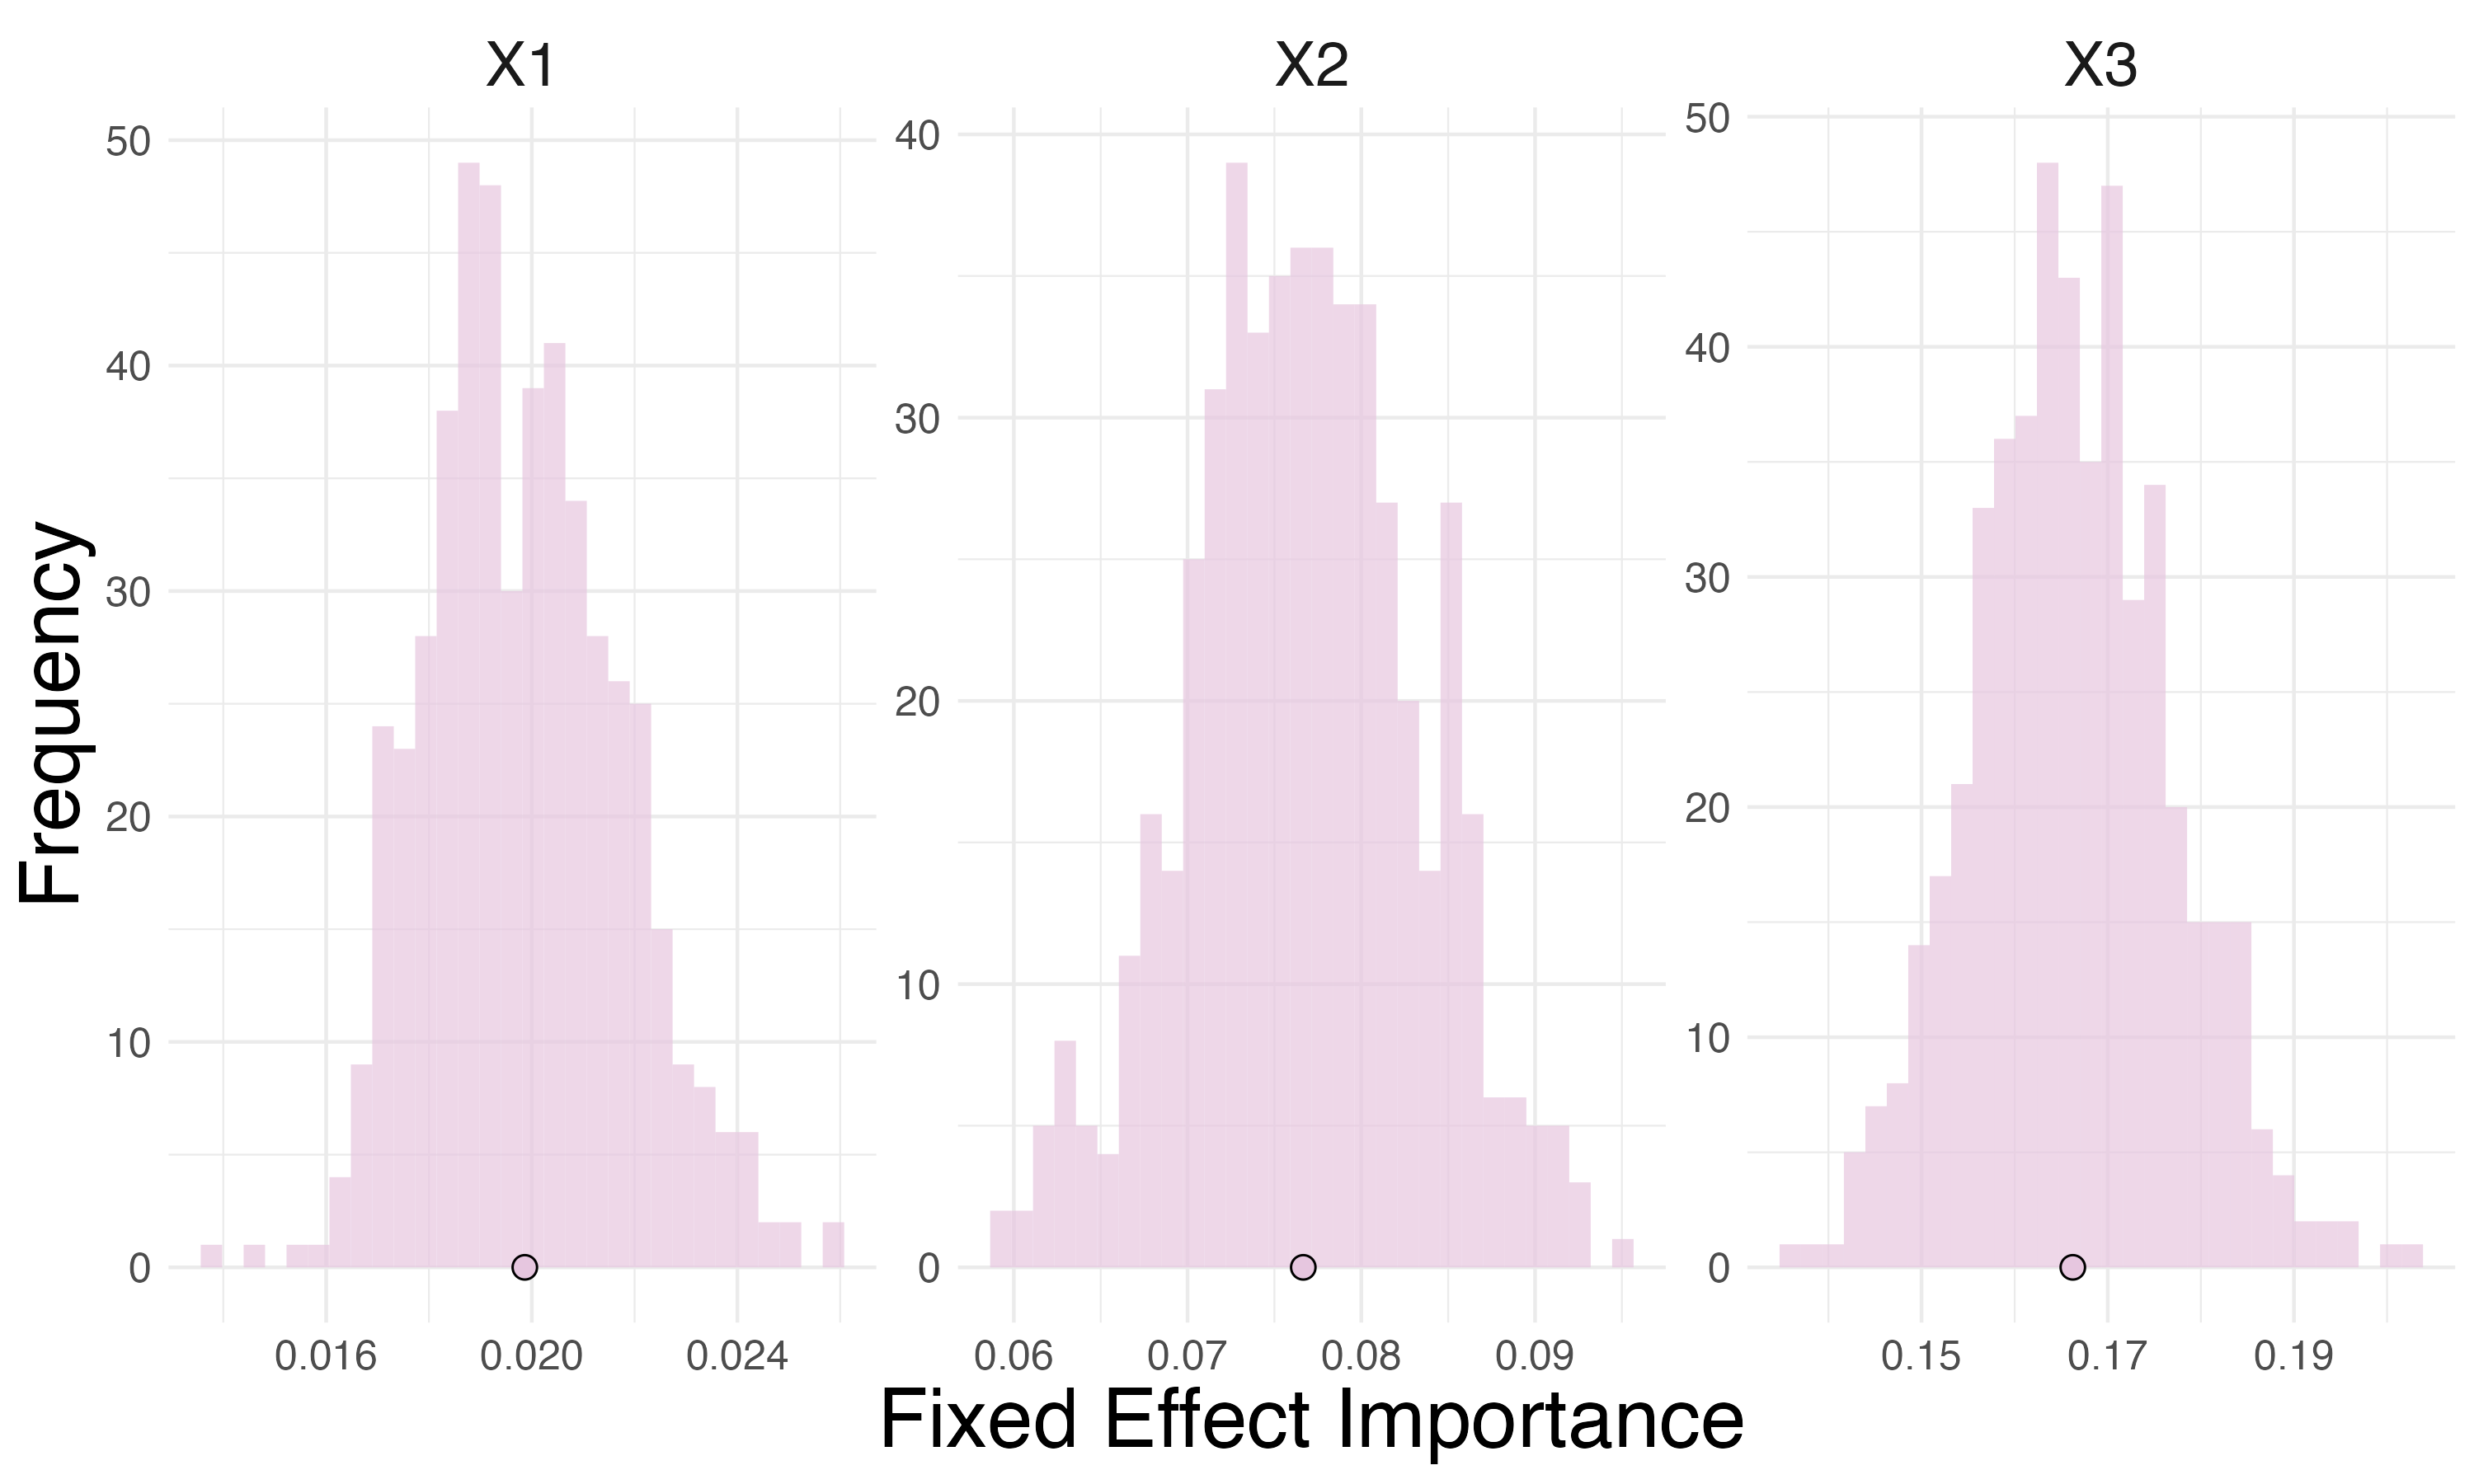
\includegraphics[width=1\linewidth]{Figures/Simulation study/Fixed_high_neg_logit.png}
%     \caption{Histogram with relative importance of the fixed effects present in the binomial regression for the different correlation levels $\rho$. The values are calculated by the Bayesian Variable Importance method from the $N_{\text{sim}}=500$ simulations in the simulation study. The true regression coefficients are $\boldsymbol{\beta}=(1, \sqrt{2}, \sqrt{3})^T$ and the vertical green line in (c) displays the expected relative importance in the case of uncorrelated data. The mean of the relative importance for all simulations is denoted at the bottom of each histogram as a circle. (a) Relative importance of the fixed effects $\mathbf{X_1},  \mathbf{X}_2, \mathbf{X}_3$ for $\rho=-0.4$.}
%     \label{fig:fixed_effects_logit_high_neg}
%   \end{figure}
%   \begin{figure}[H]\ContinuedFloat
%     \centering
%     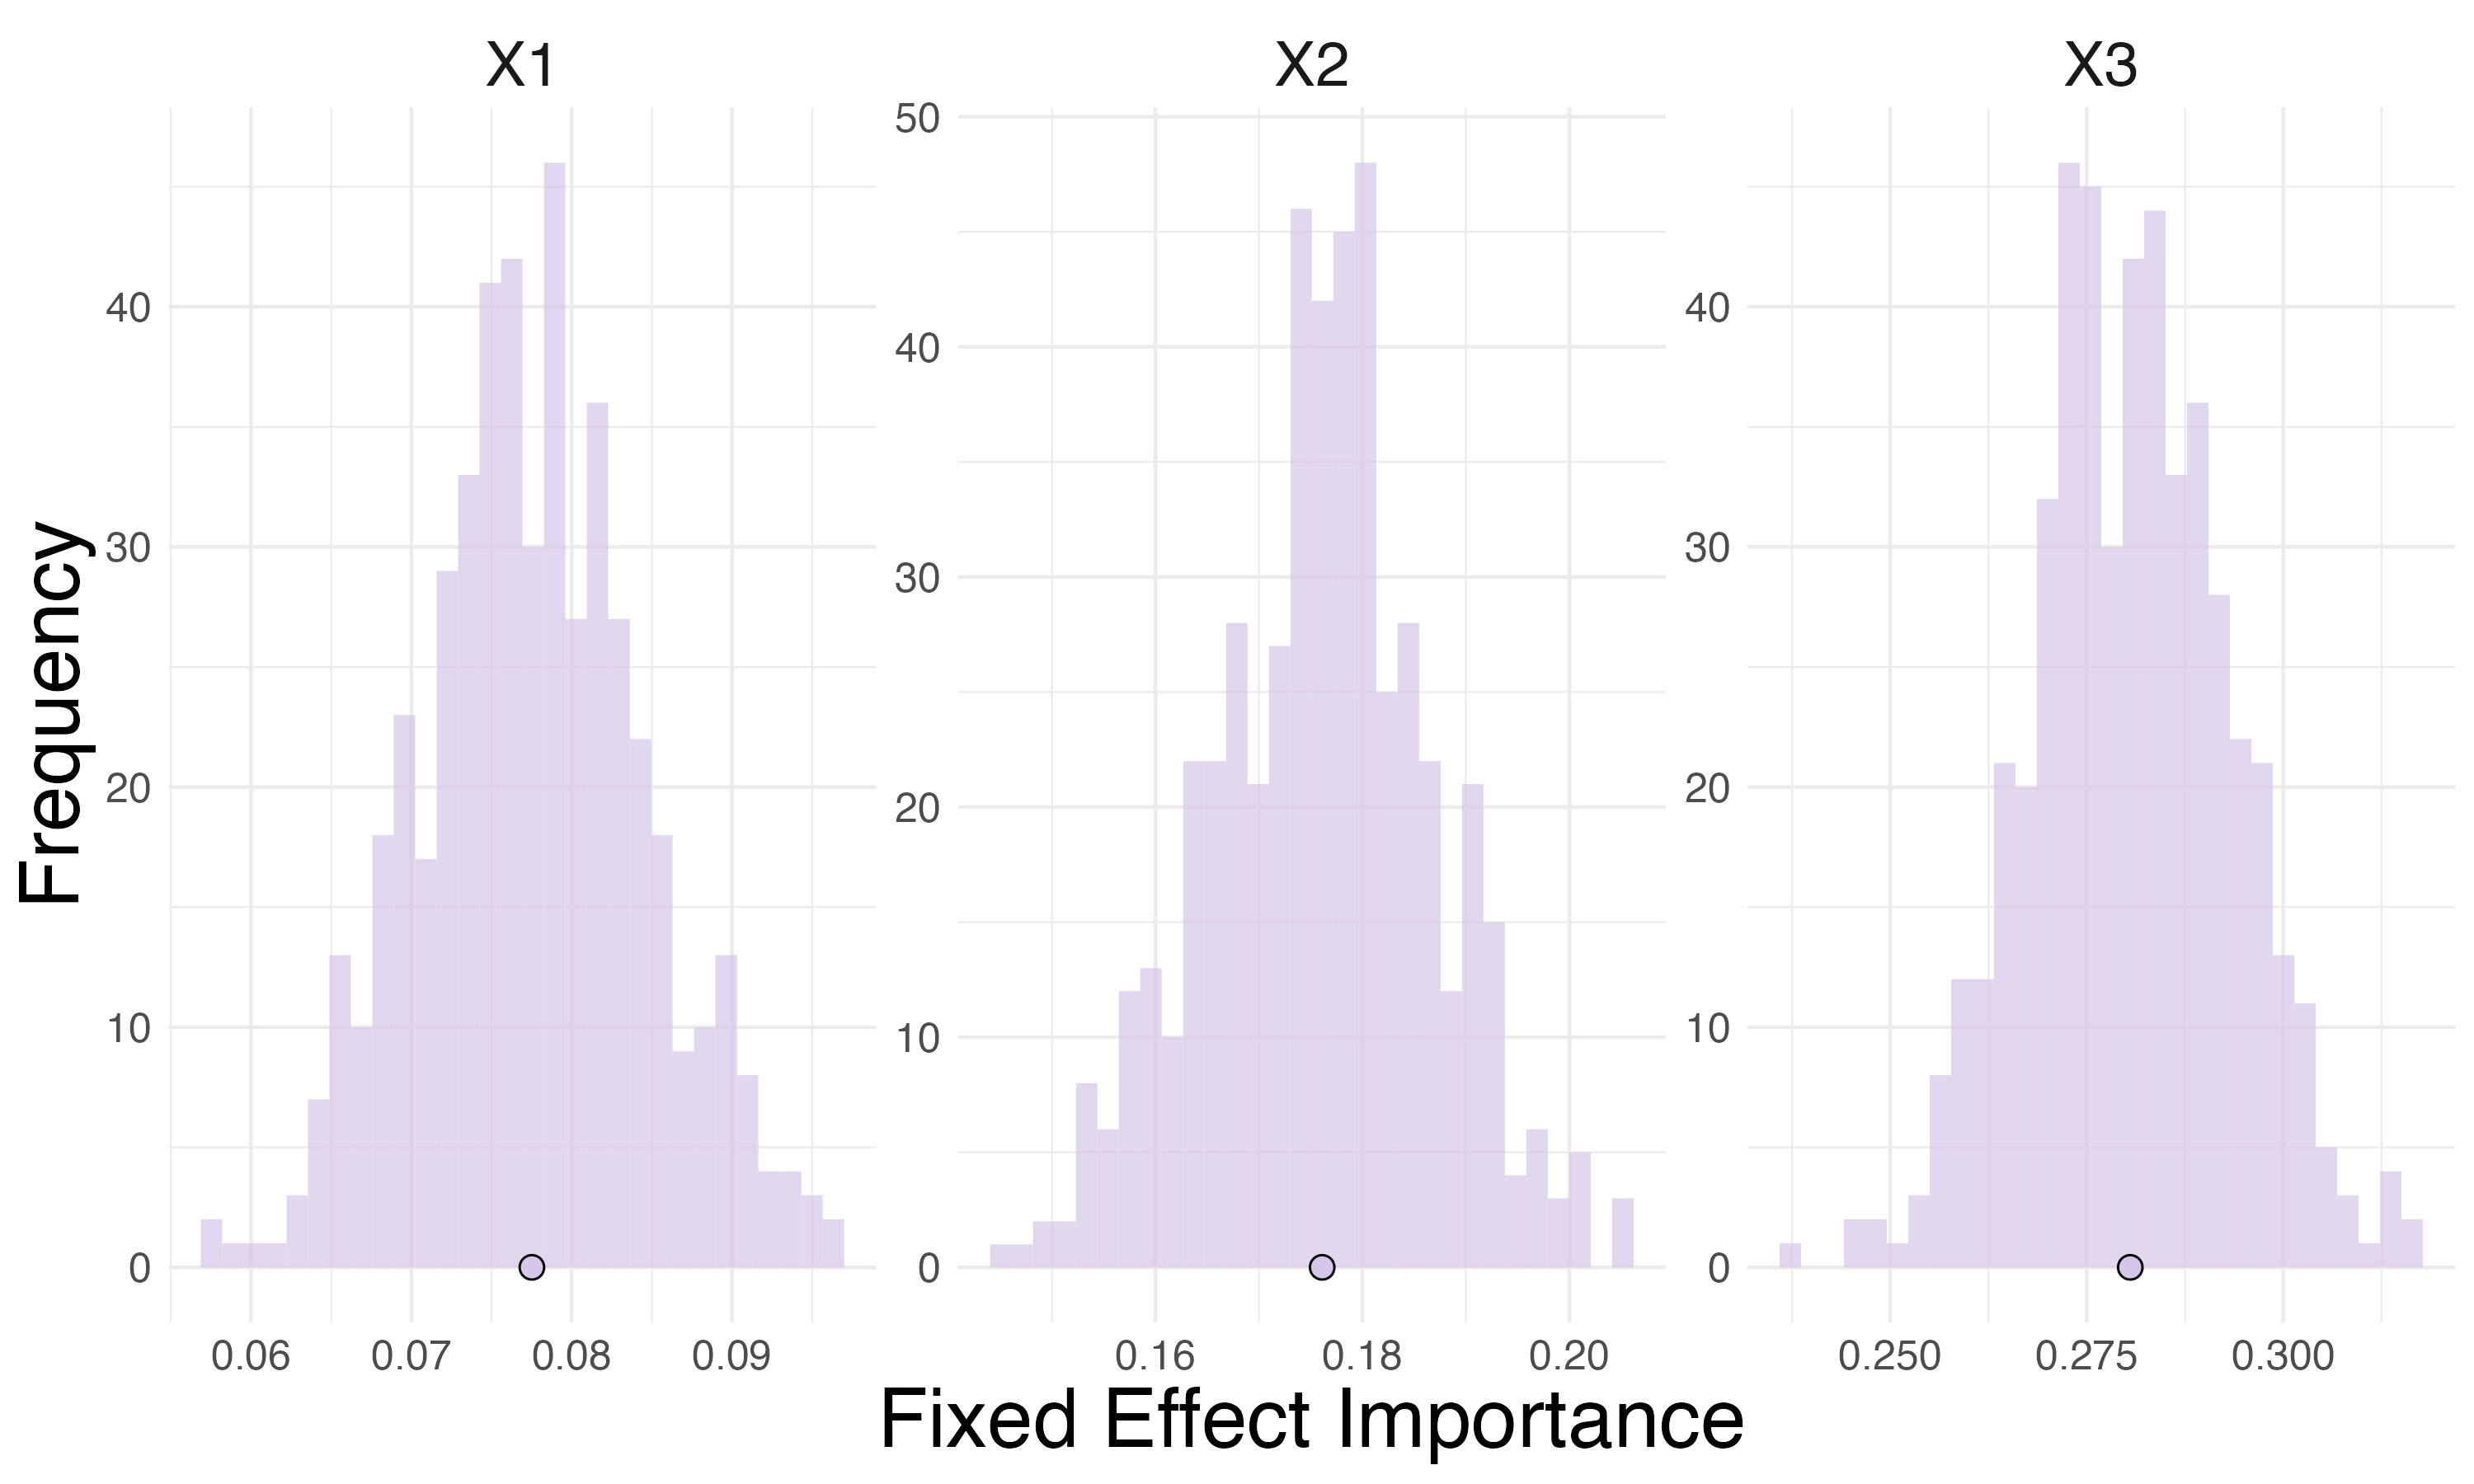
\includegraphics[width=1\linewidth]{Figures/Simulation study/Fixed_low_neg_logit.png}
%     \caption{(b) Relative importance of $\mathbf{X_1},  \mathbf{X}_2, \mathbf{X}_3$ for $\rho=-0.1$.}
%     \label{fig:fixed_effects_logit_low_neg}
%   \end{figure}
%   \begin{figure}[H]\ContinuedFloat
%     \centering
%     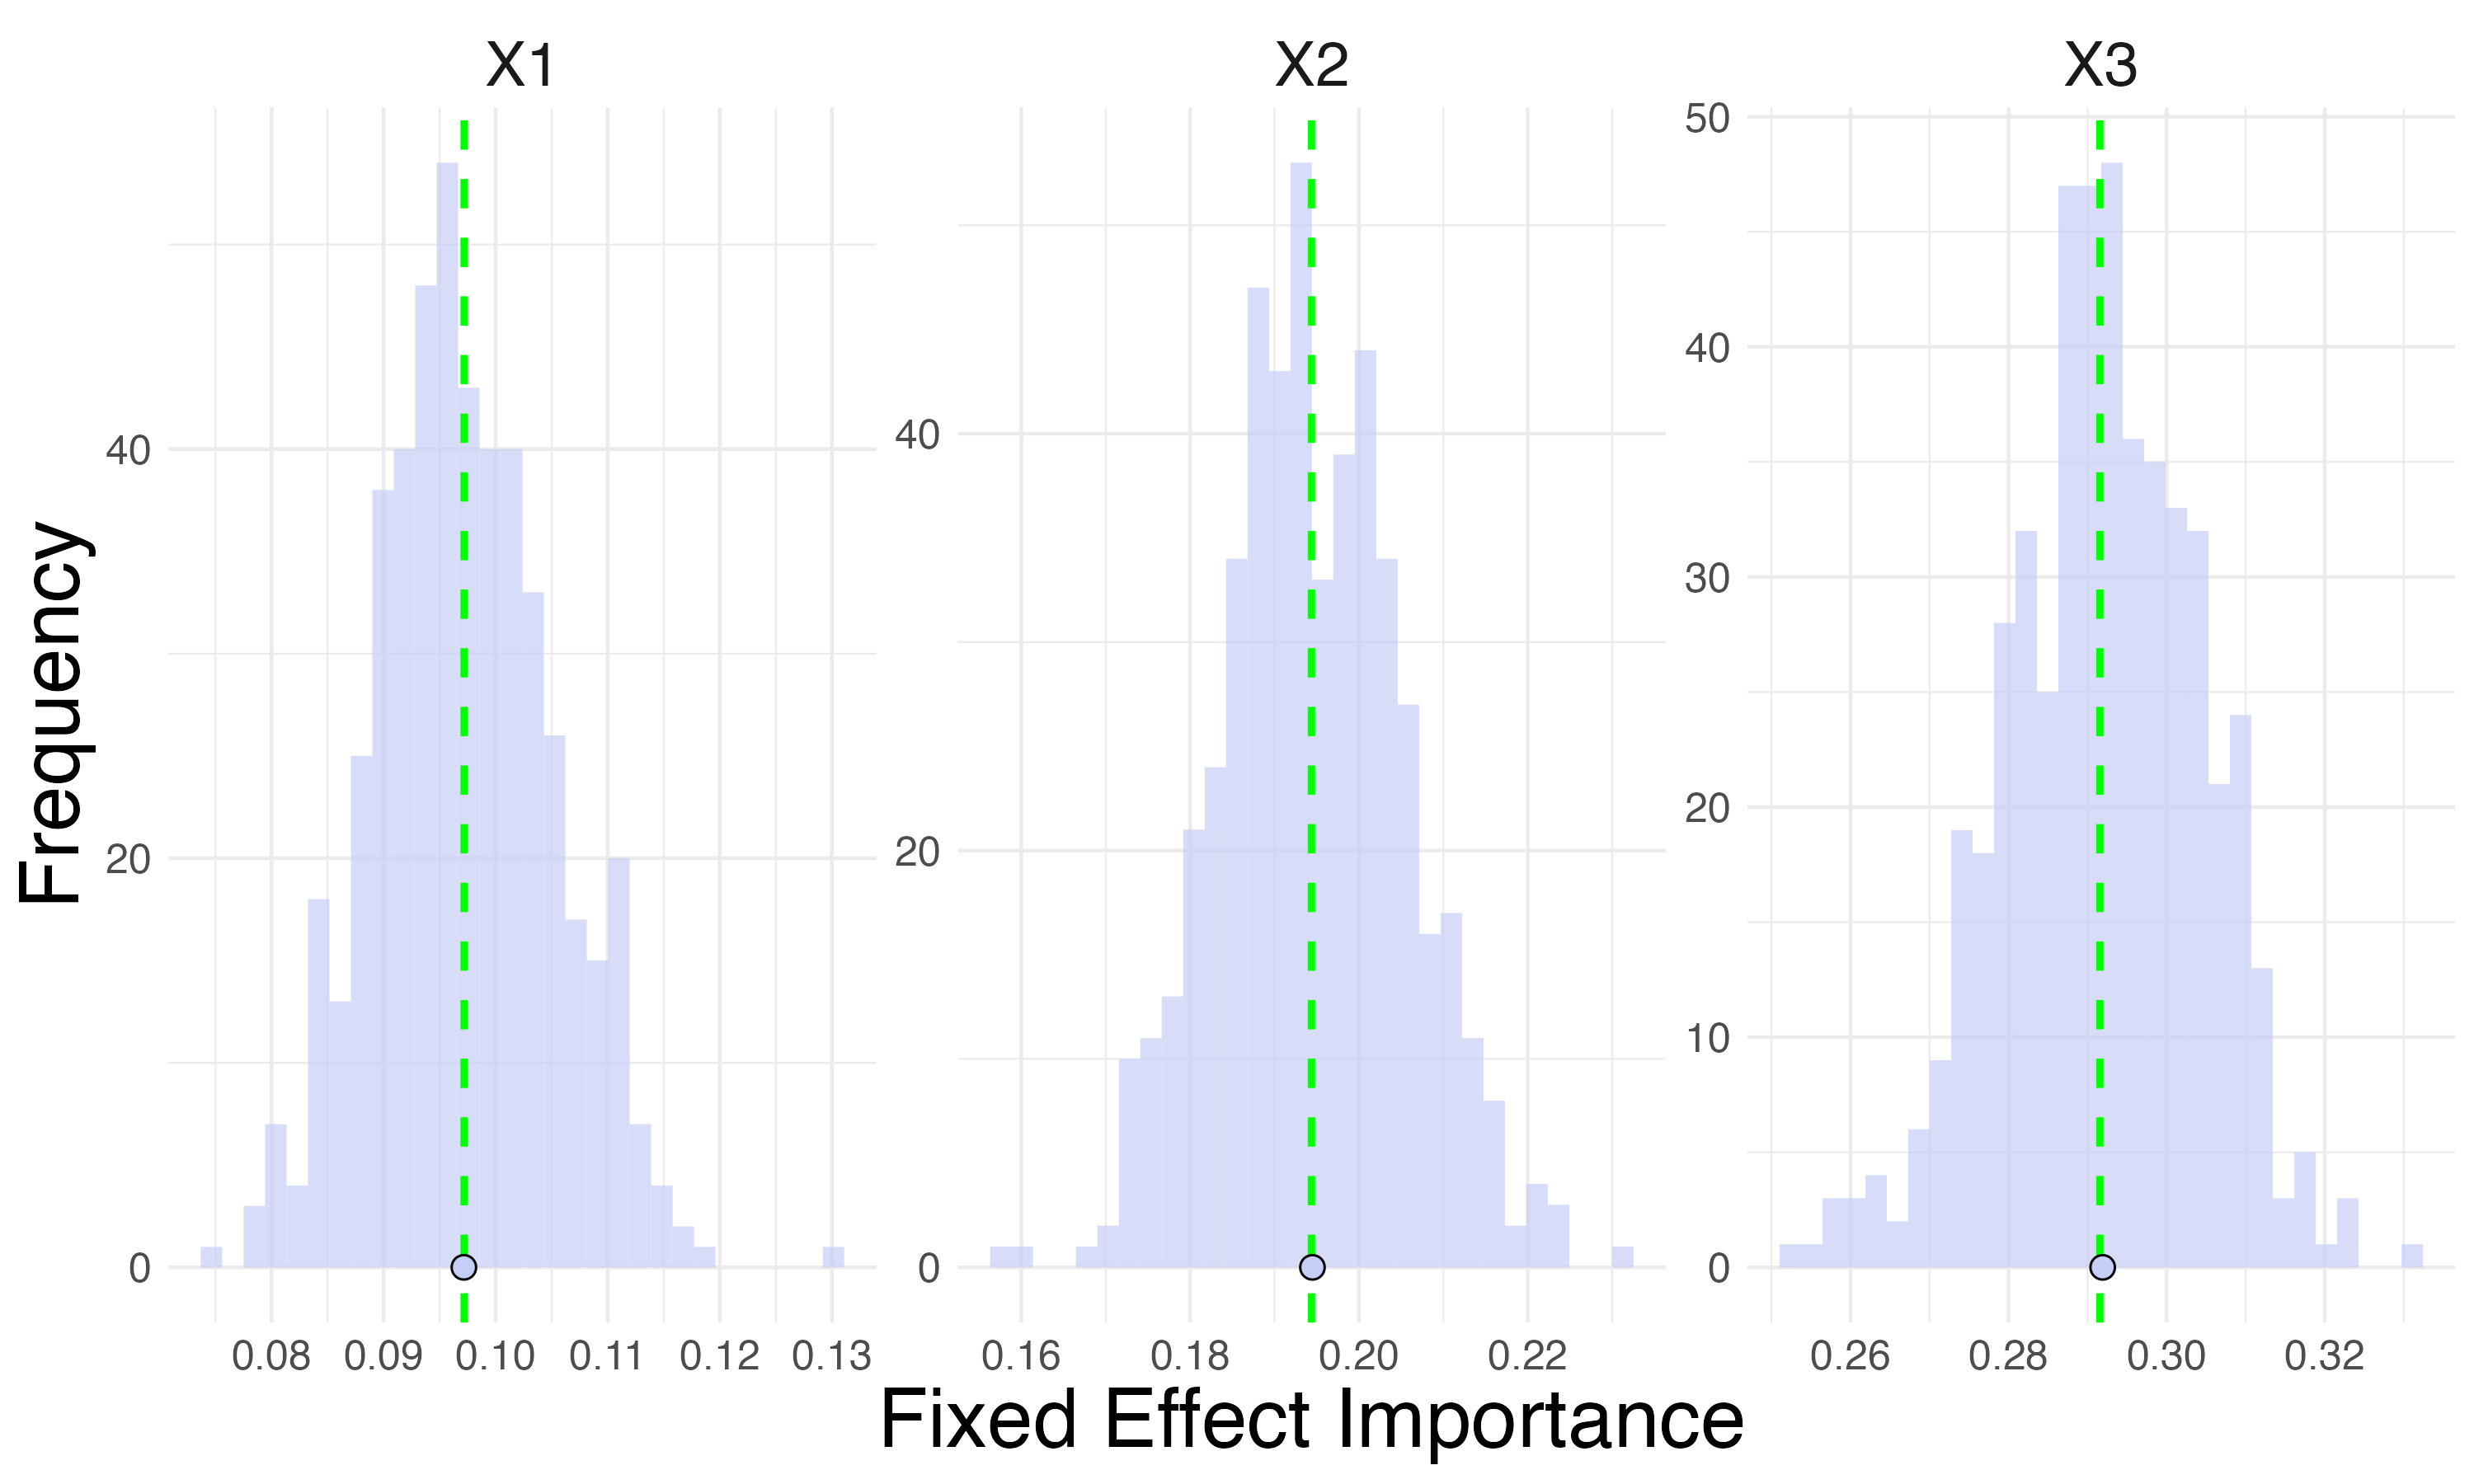
\includegraphics[width=1\linewidth]{Figures/Simulation study/Fixed_no_logit.png}
%     \caption{(c) Relative importance of $\mathbf{X_1},  \mathbf{X}_2, \mathbf{X}_3$ for $\rho=0$.}
%     \label{fig:fixed_effects_logit_no}
%   \end{figure}
%   \begin{figure}[H]\ContinuedFloat
%     \centering
%     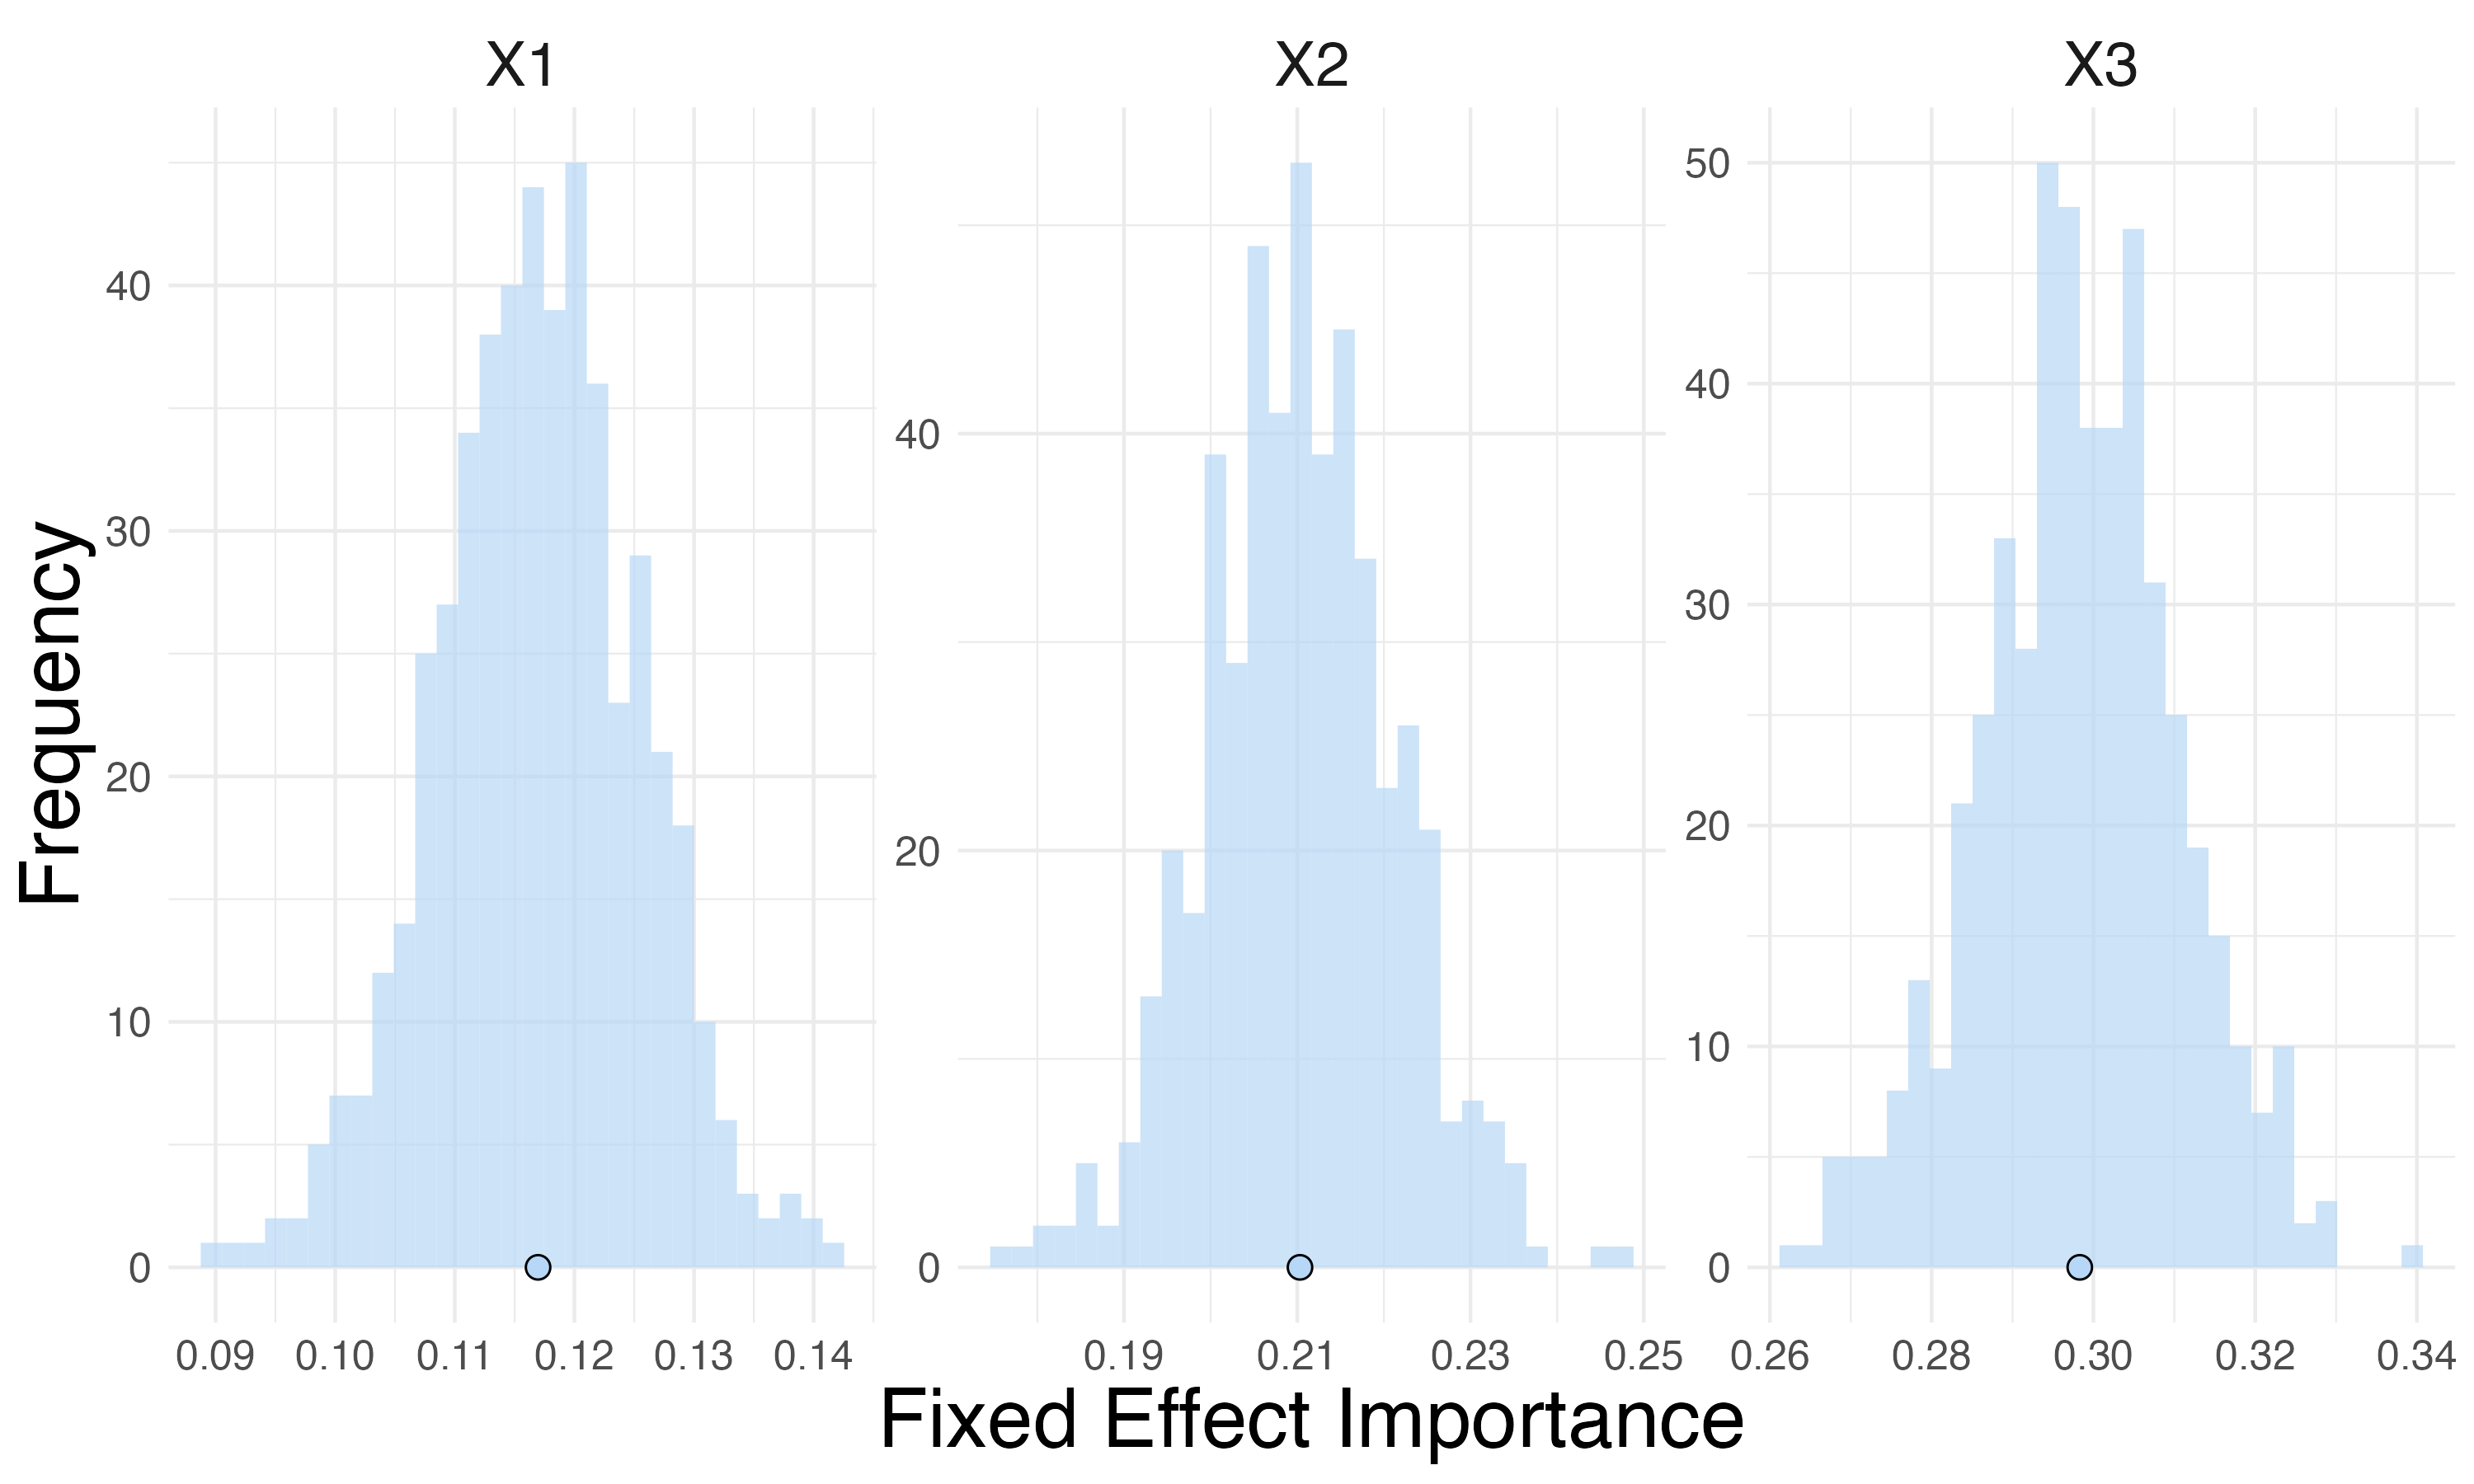
\includegraphics[width=1\linewidth]{Figures/Simulation study/Fixed_low_pos_logit.png}
%     \caption{(d) Relative importance of $\mathbf{X_1},  \mathbf{X}_2, \mathbf{X}_3$ for $\rho=0.1$.}
%     \label{fig:fixed_effects_logit_low_pos}
%   \end{figure}
%   \begin{figure}[H]\ContinuedFloat
%     \centering
%     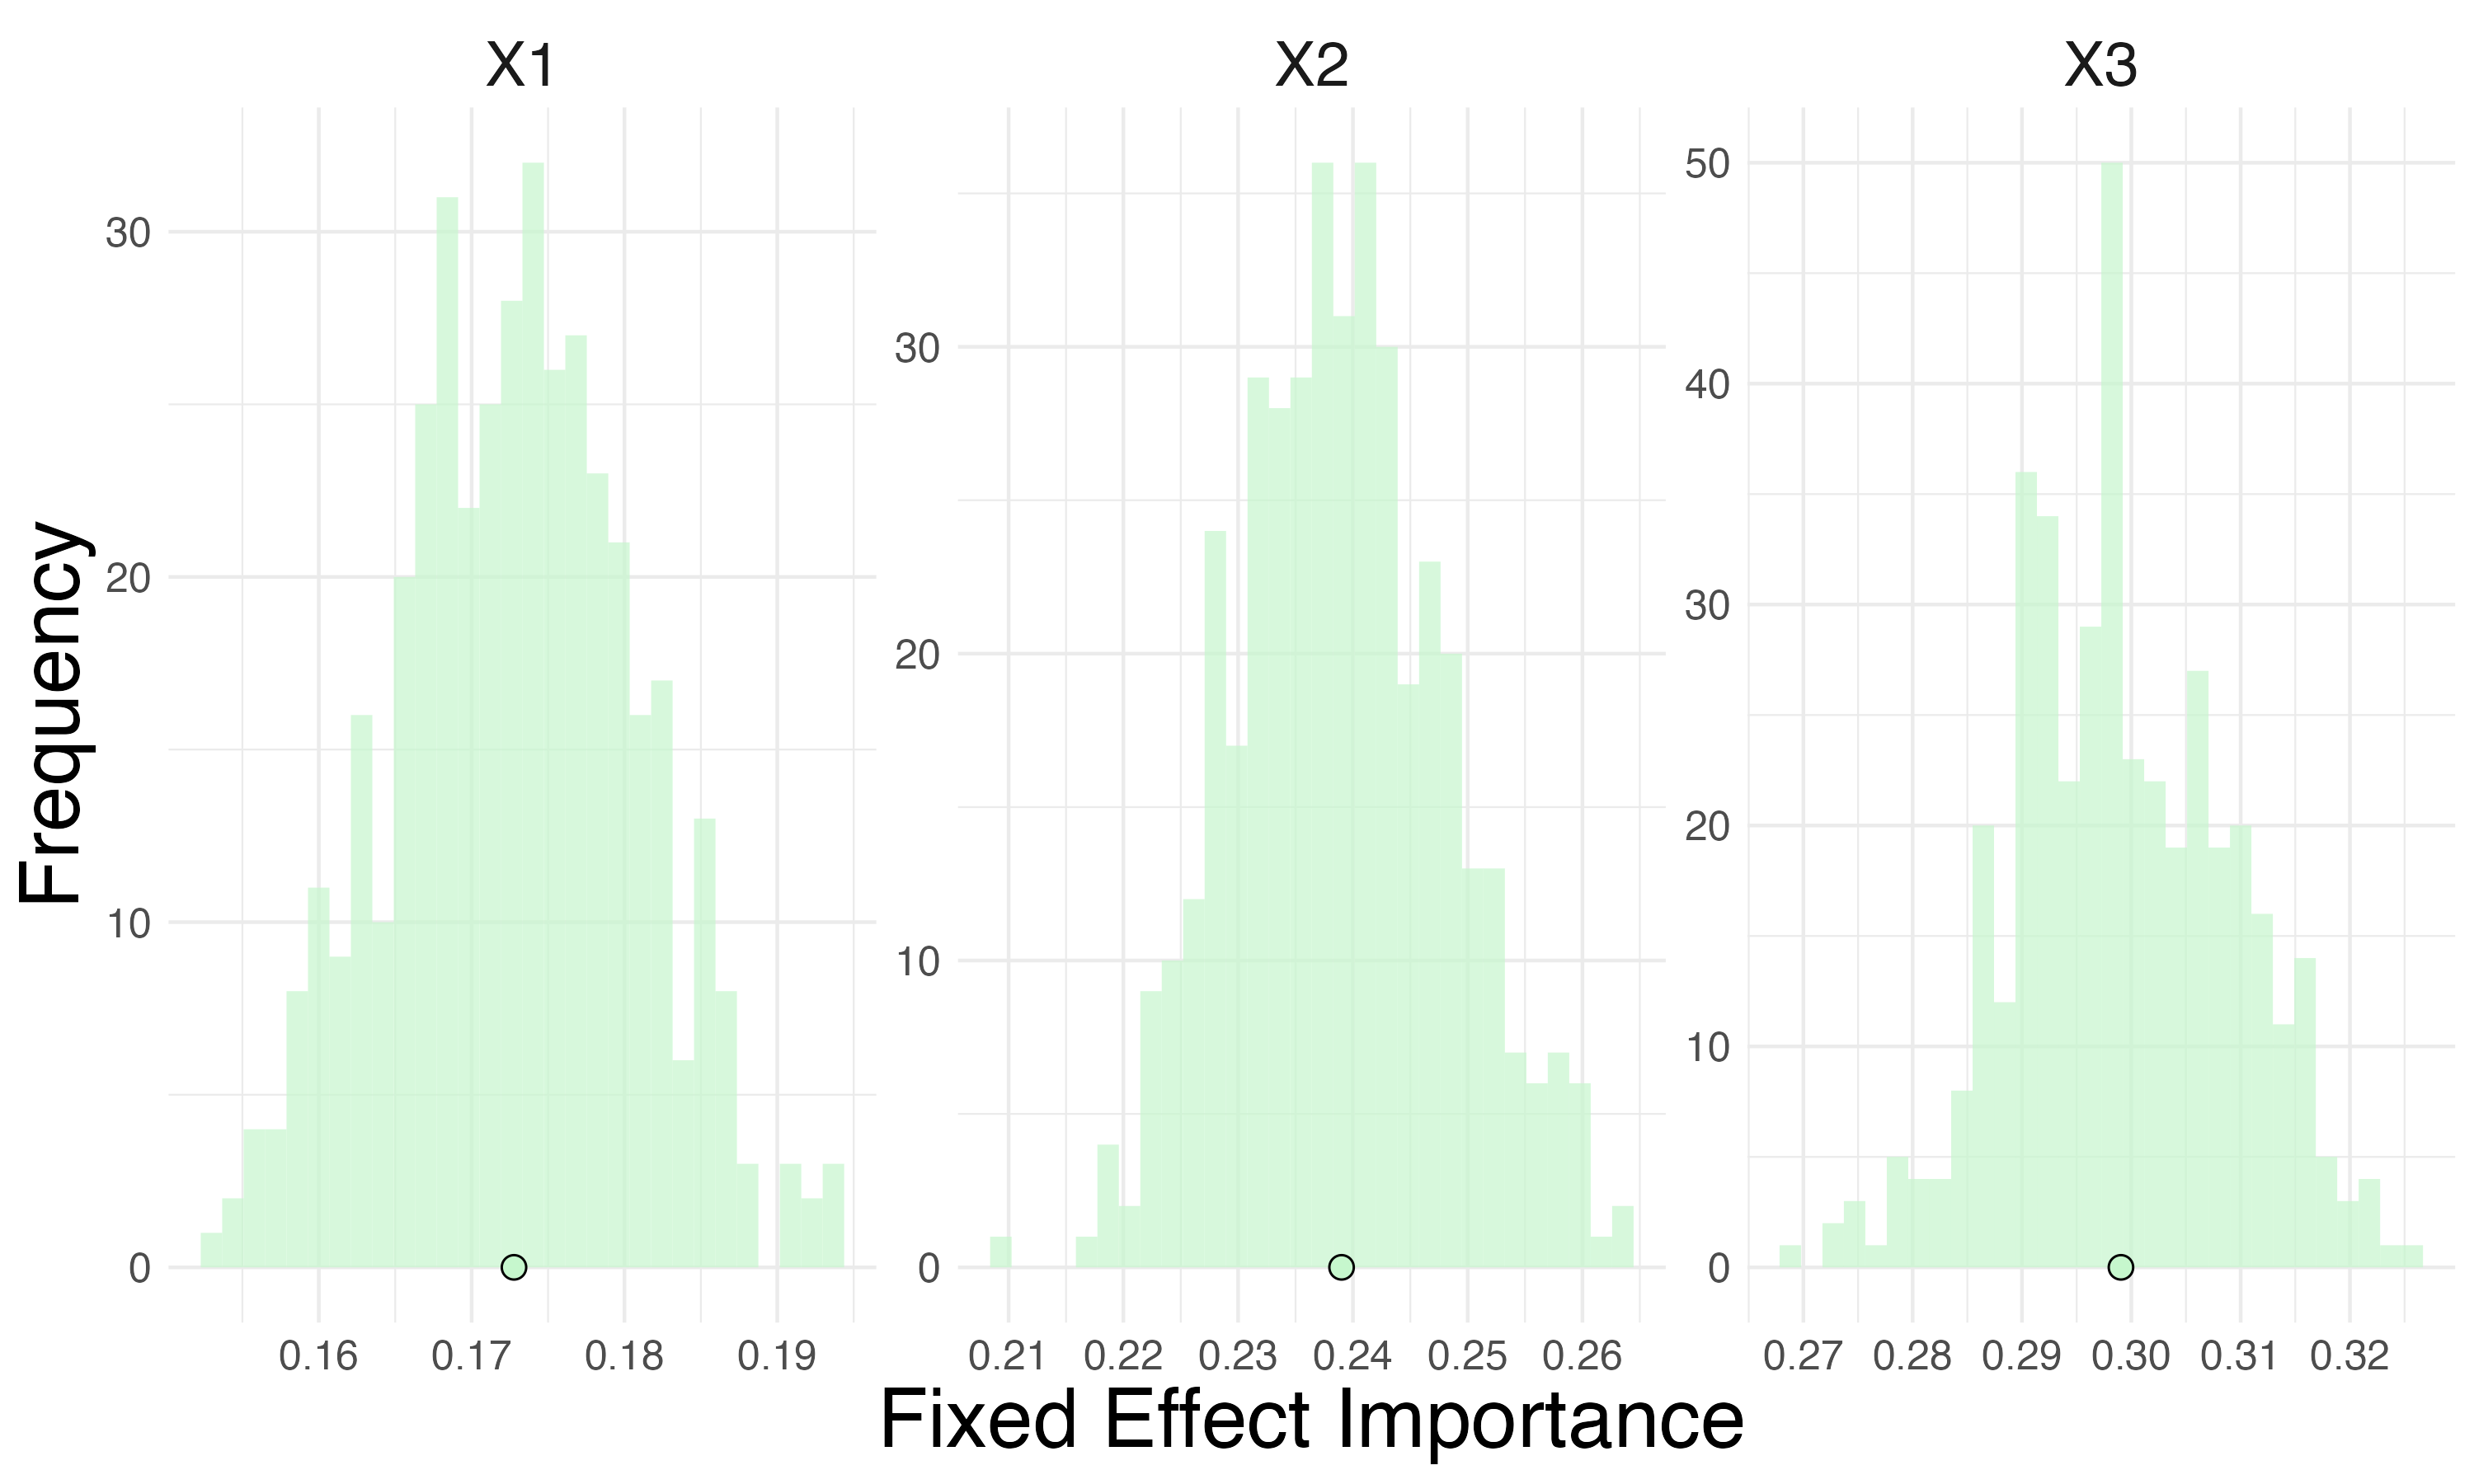
\includegraphics[width=1\linewidth]{Figures/Simulation study/Fixed_high_pos_logit.png}
%     \caption{(e) Relative importance of $\mathbf{X_1},  \mathbf{X}_2, \mathbf{X}_3$ for $\rho=0.4$.}
%     \label{fig:fixed_effects_logit_high_pos}
% \end{figure}
% \begin{figure}[H]
%   \centering
%   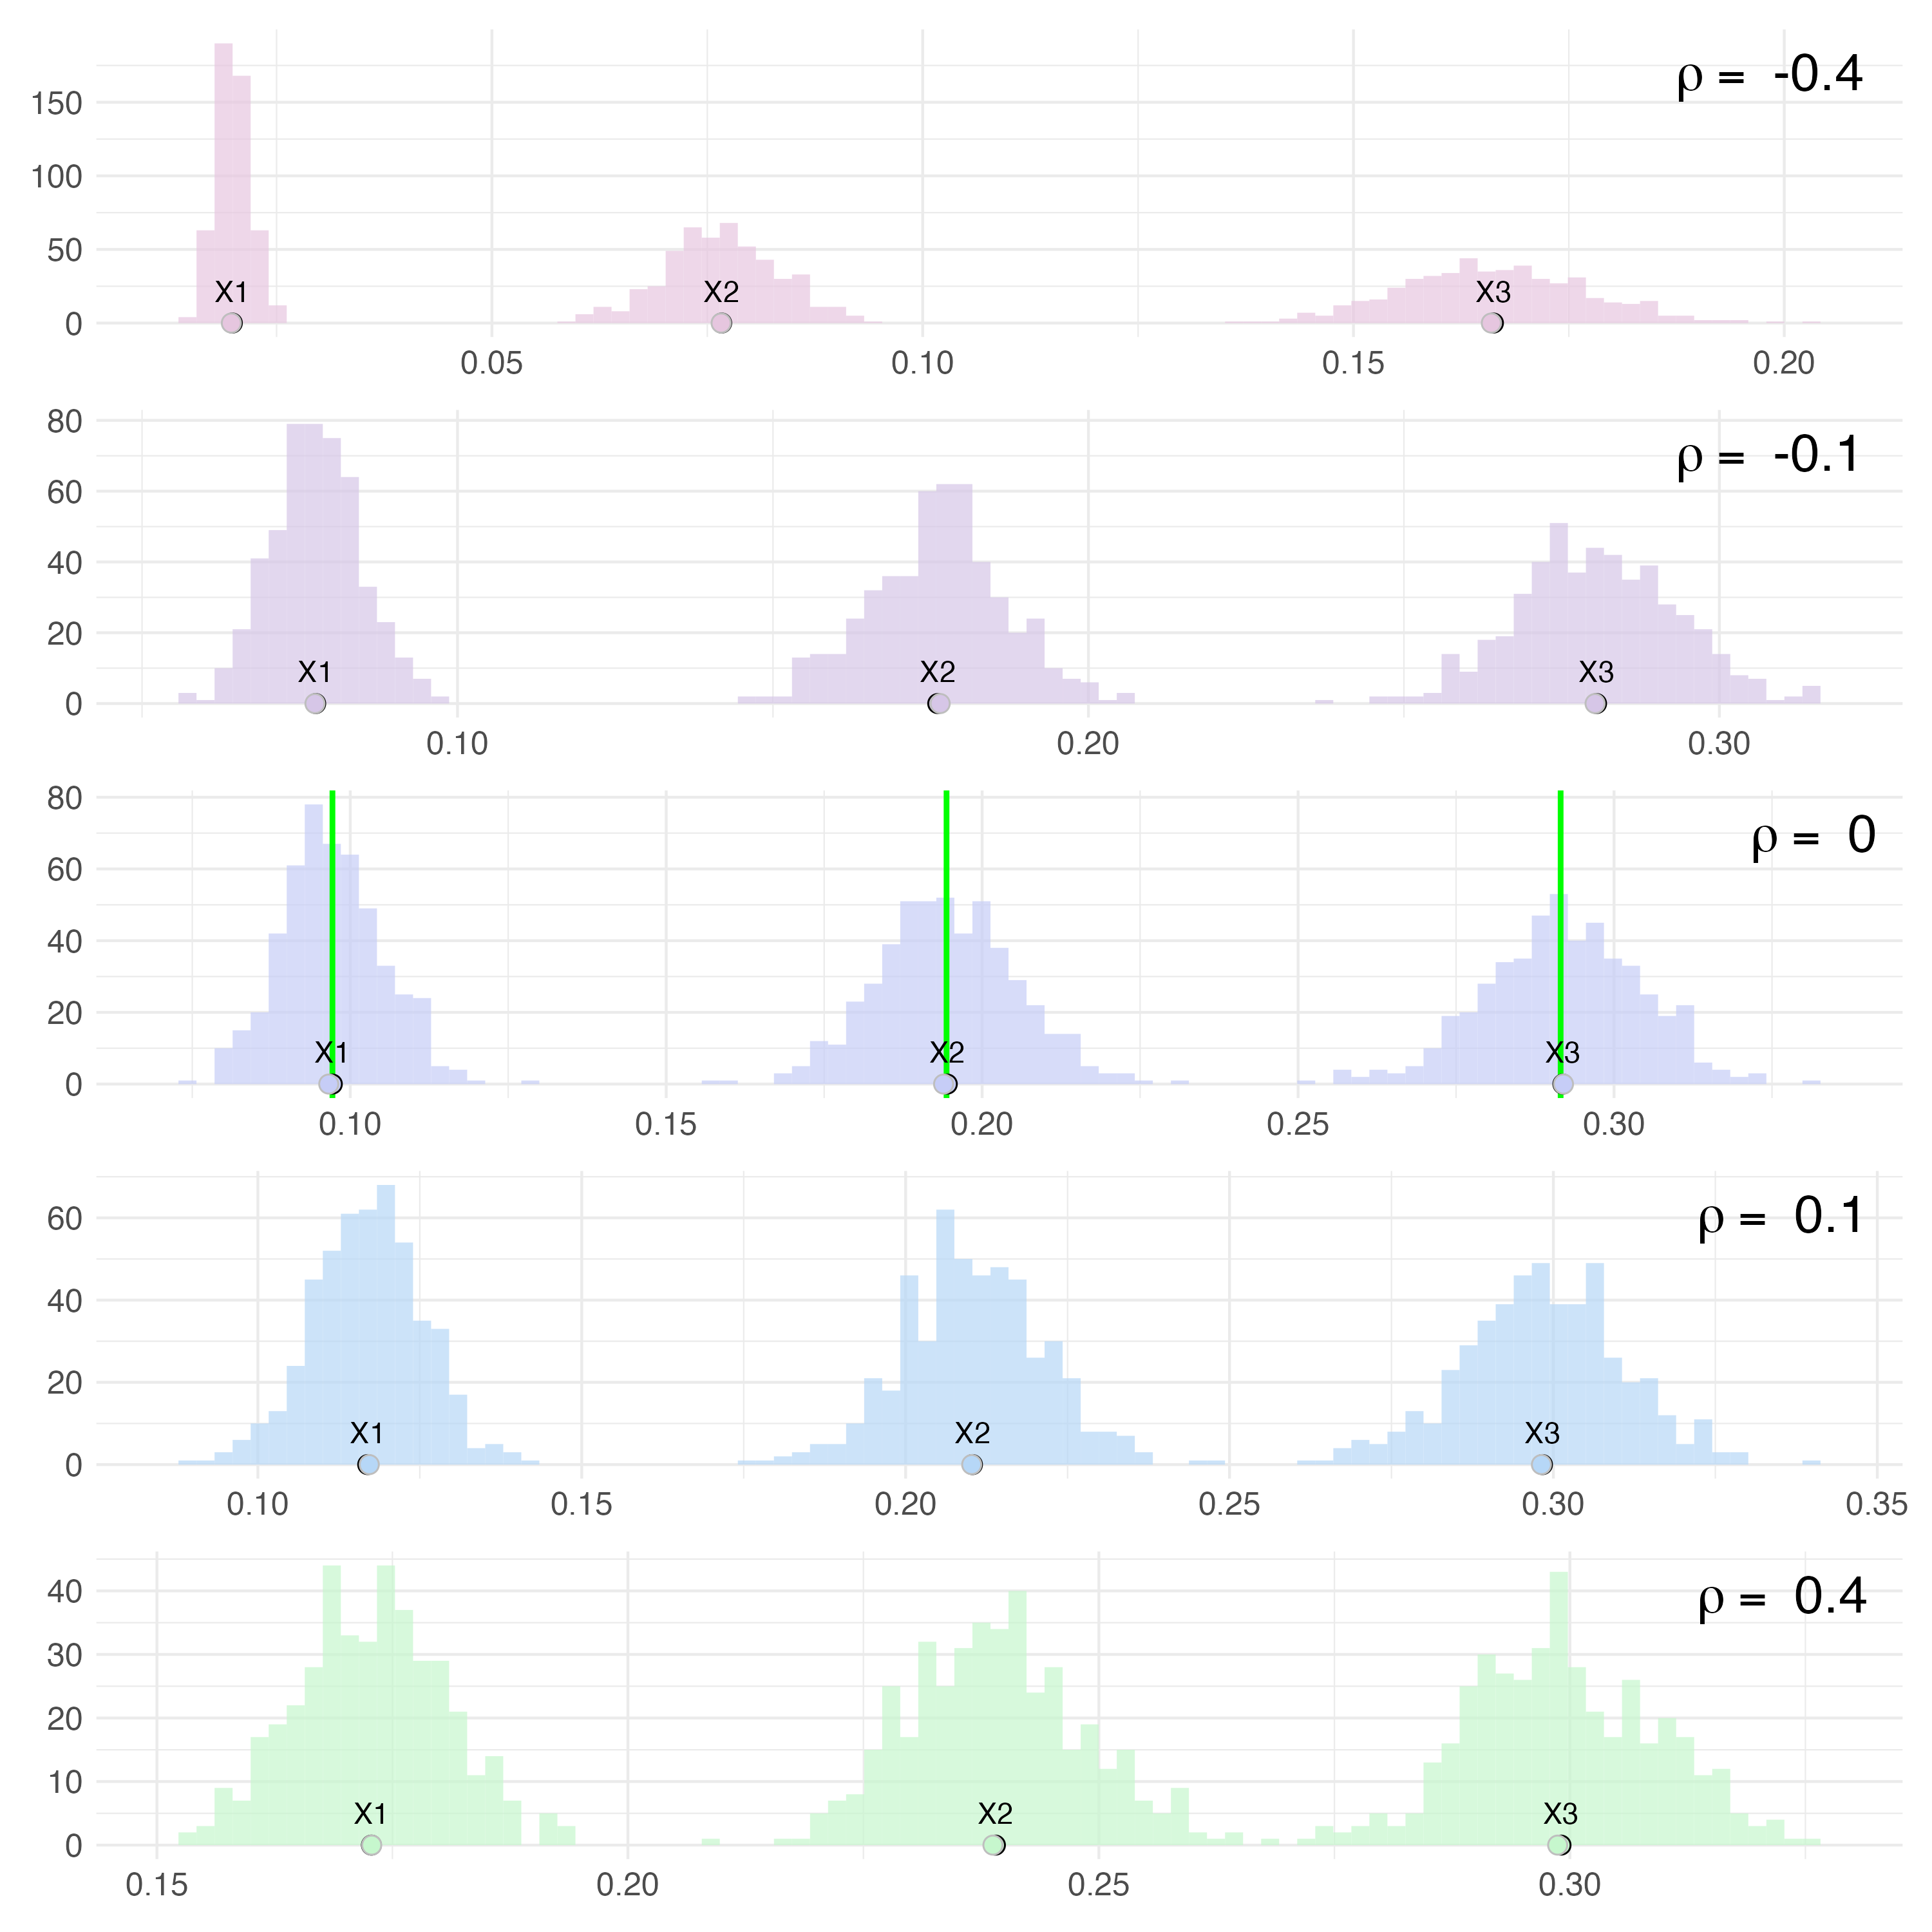
\includegraphics[width=1.5\linewidth]{Figures/Simulation study/Fixed_combined_logit.png}
%   \caption{(f) Relative importance of the fixed effects $\mathbf{X_1},  \mathbf{X}_2, \mathbf{X}_3$ for $\rho=0.4$.}
%   \label{fig:fixed_combined_logit}
% \end{figure}
\begin{figure}[H]
  \centering
  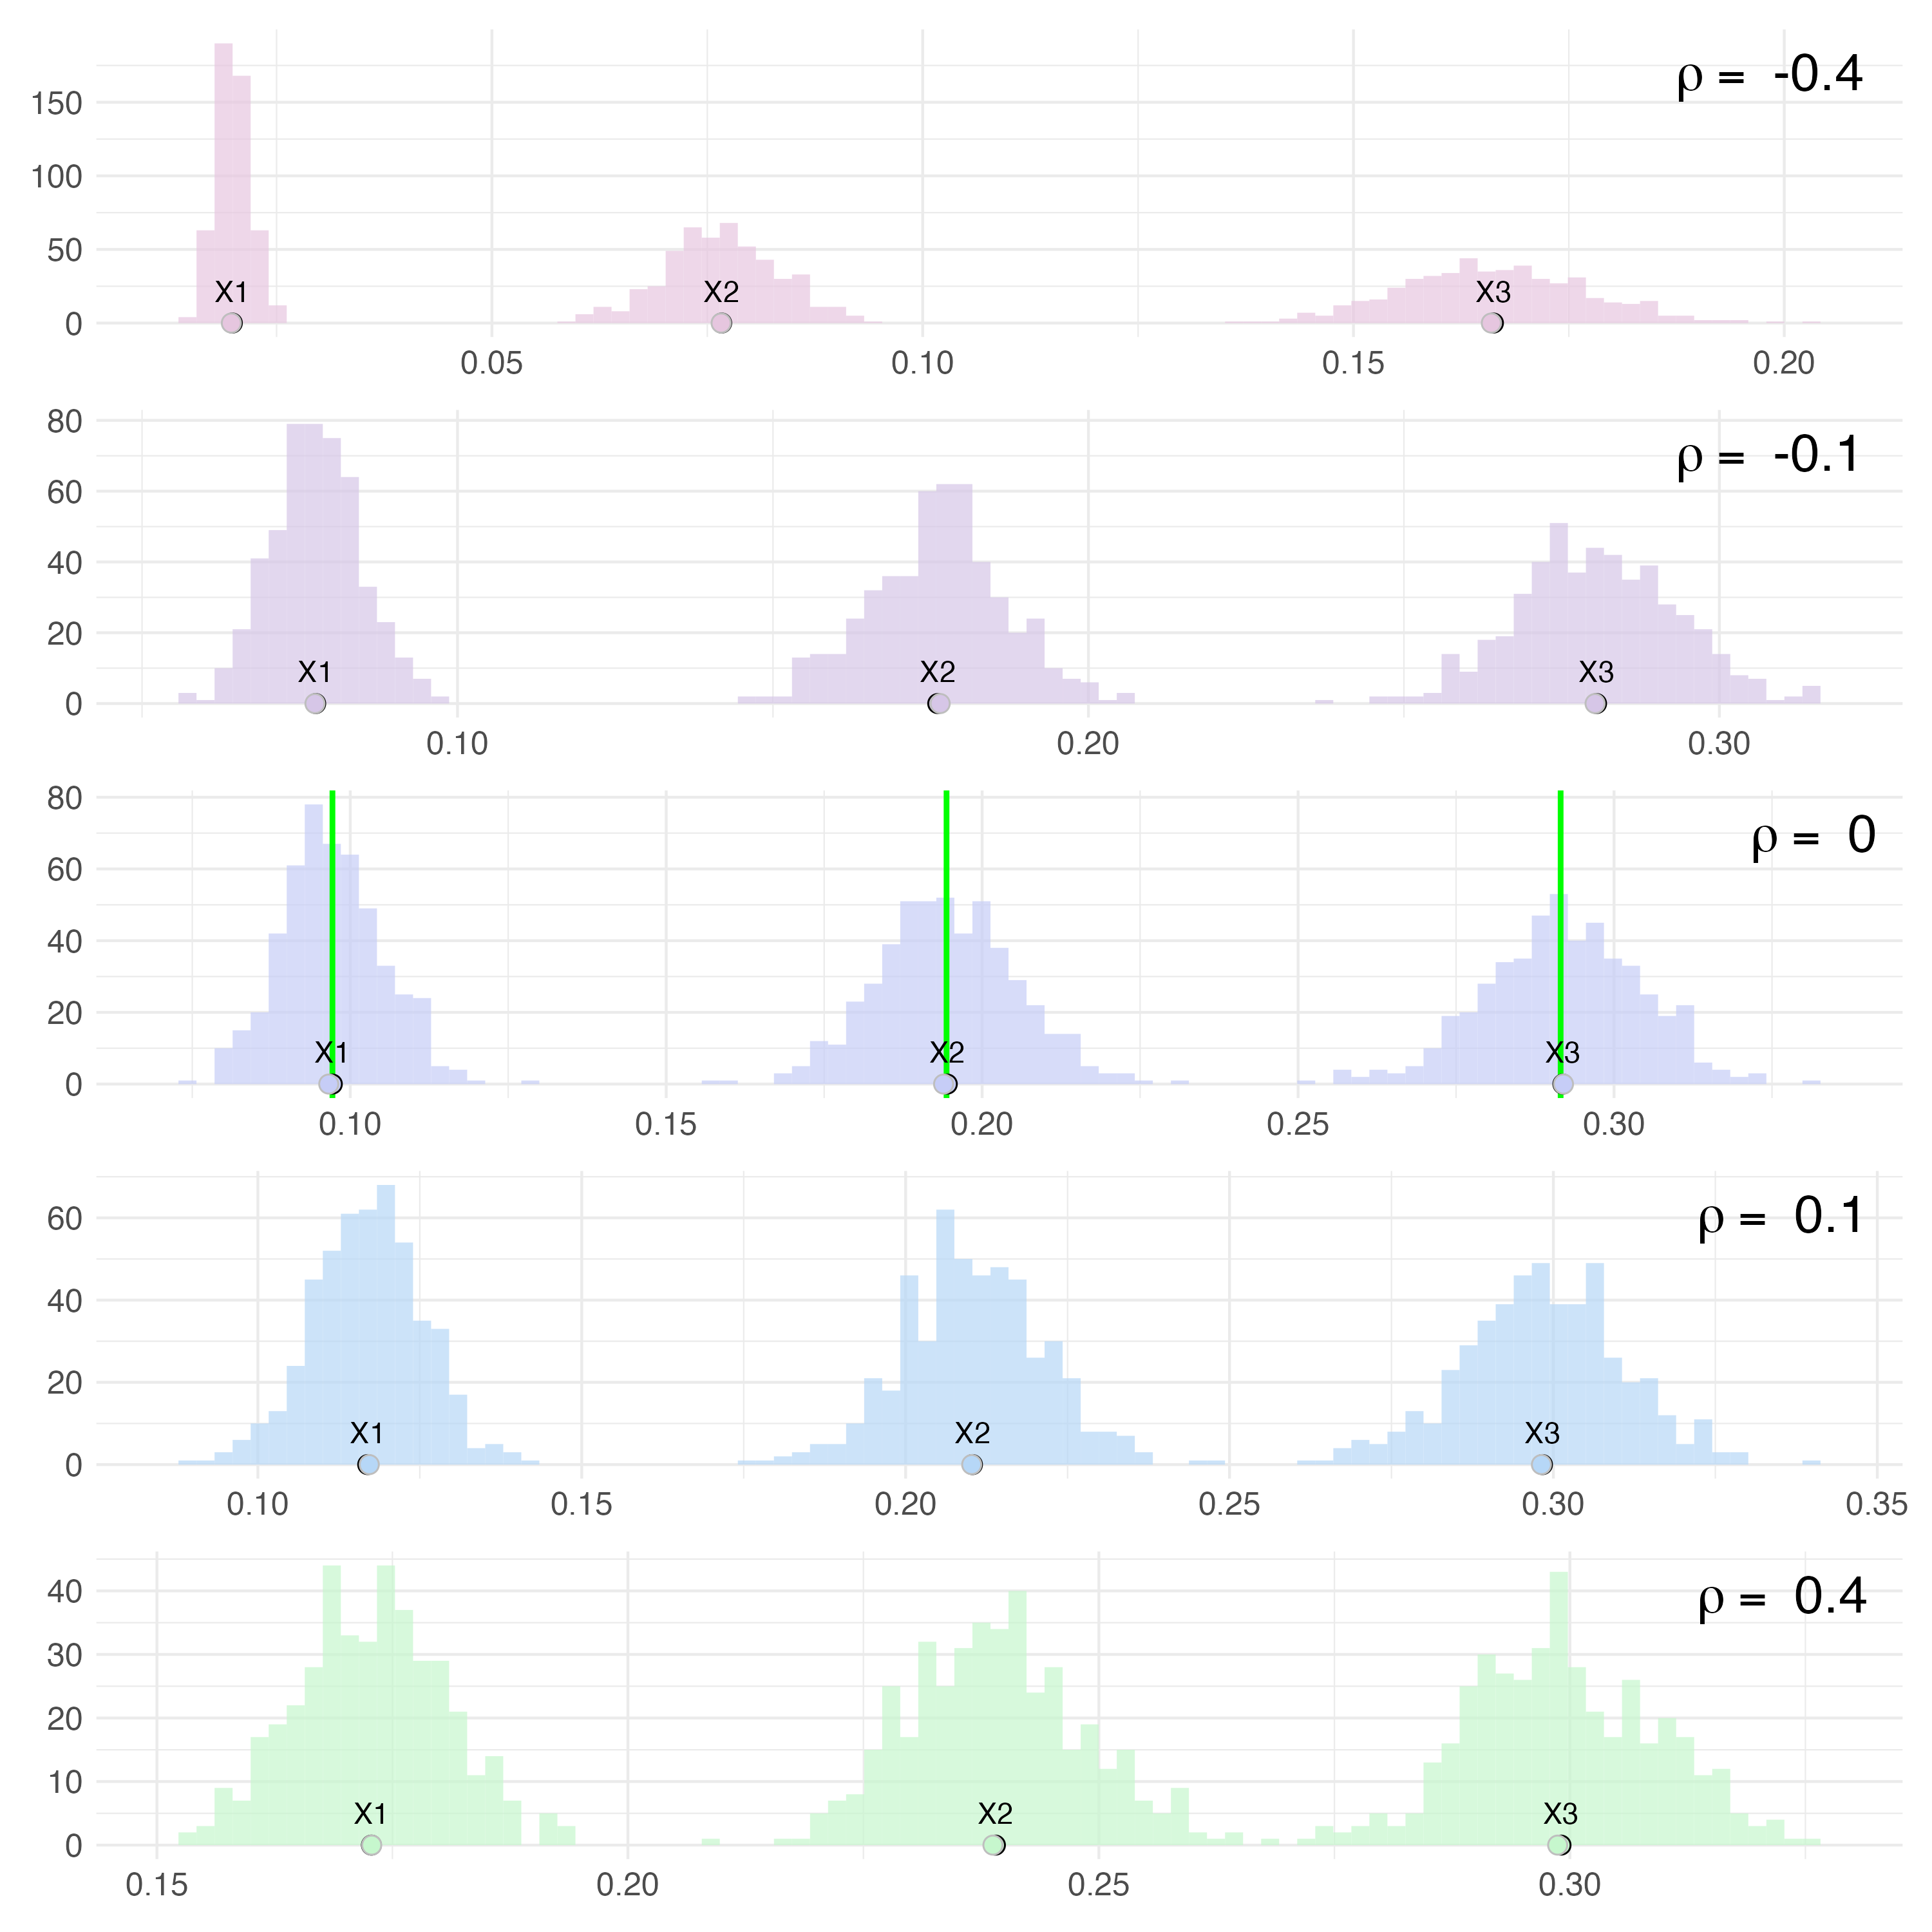
\includegraphics[width=1.1\linewidth]{Figures/Simulation study/Fixed_combined_logit.png}
  \caption{Histogram with relative importance of the fixed effects present in the binomial regression for the different correlation levels $\rho=-0.4$ (top), $\rho=-0.1$ (second from the top), $\rho=0$ (middle), $\rho=0.1$ (second from bottom) and $\rho=0.4$ (bottom). The values are calculated by the Bayesian Variable Importance method from the $N_{\text{sim}}=500$ simulations in the simulation study. The true regression coefficients are $\boldsymbol{\beta}=(1, \sqrt{2}, \sqrt{3})^T$ and the vertical green line for $\rho=0$ displays the expected relative importance in the case of uncorrelated data. The mean of the relative importance for all simulations is denoted at the bottom of each histogram as a circle.}
  \label{fig:fixed_combined_logit}
\end{figure}
  %\label{fig:fixed_effects_logit}
%\end{figure}
\subsubsection{Random effect}
The sampled posterior importances for the random effect in the logit model (\Cref{fig:relimp_random_logit}) all seem to be roughly normally distributed around the mean. It is clear that when the correlation in fixed effects go from negative to positive, the estimated importance of the random effect shrinks. Specifically, when $\rho=-0.4$ the average estimate of relative importance for the random effect is $0.1688$ compared to only $0.0663$ when $\rho=0.4$. This naturally occurs as the variance contribution from the random effect should be held constant for the correlation levels, and the variance contribution from the fixed effects rise as the correlation increases. Therefore the proportion of variance explained, which is our definition of relative variable importance, will decrease for the random effect. For $\rho=0$ we see that the average relative importance estimate lies very near the expected value of $0.0972$ as shown in \Cref{table:2}. The orange dot at the bottom of the histograms in \Cref{fig:relimp_random_logit} displays the estimated relative importance of the fixed effect from the \texttt{rptR} package, and we see that the estimates are quite close to the mean of the BVI method. The largest difference from the BVI and the \texttt{rptR} package is $0.0351$ and are found when $\rho=-0.4$. It can be noted that the authors of the \texttt{rptR} package \citep{Stoffel2017rptR} write in the vignette that any model fit with the package will automatically be fit with a term to account for additive overdispersion. This may explain the difference in the relative importance estimates, as the simulated data is not overdispersed.
\\
\\
\begin{figure}[H]
  \centering
    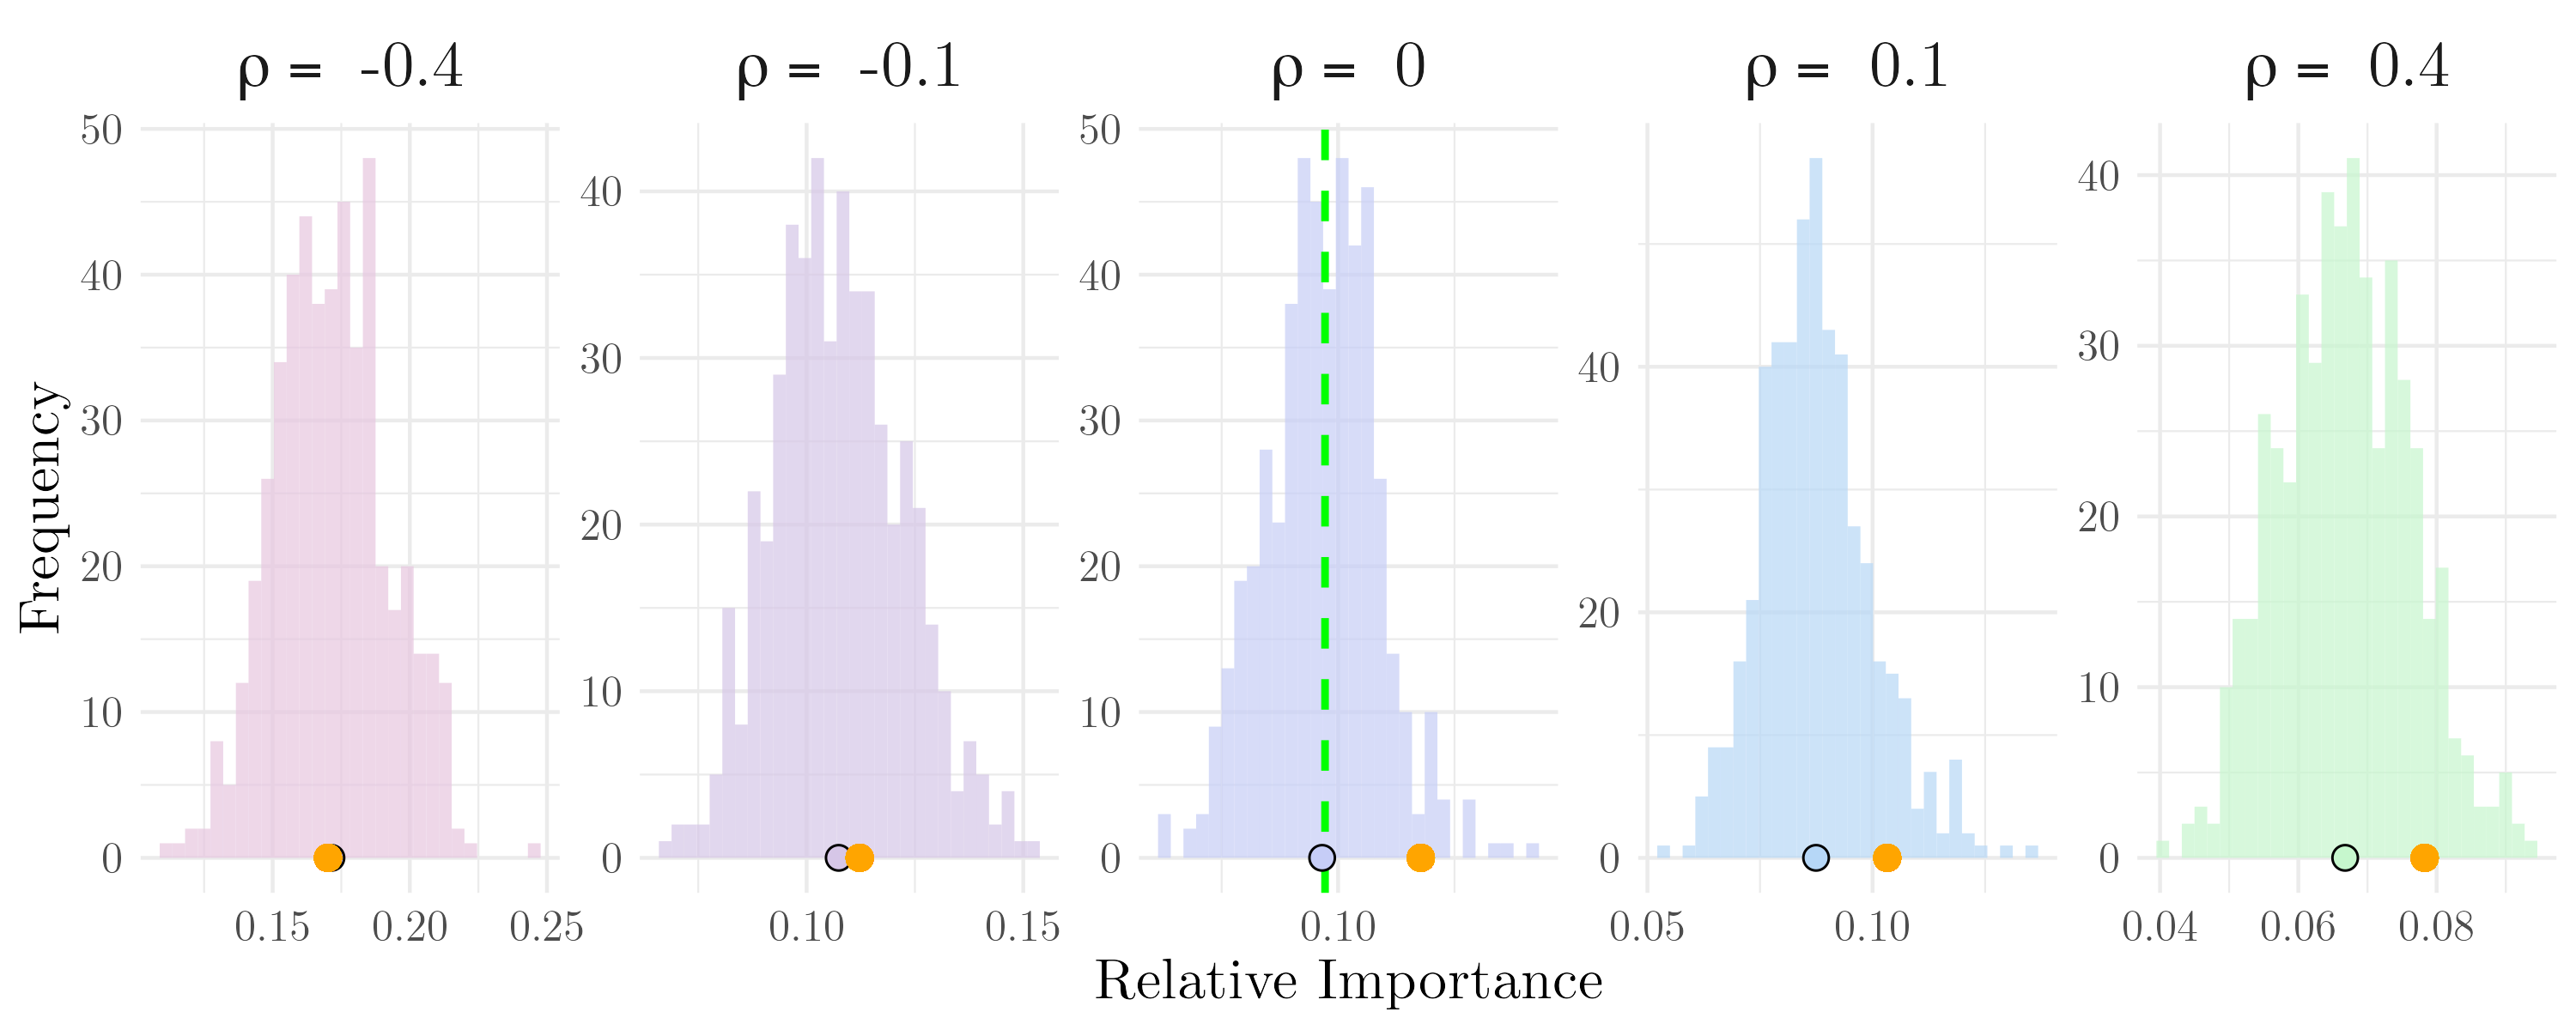
\includegraphics[width=1\linewidth]{Figures/Simulation study/Random_logit.png}
    \caption{Histogram with values from the BVI method for each of the $N_{\text{sim}}=500$ simulations, estimating relative importance of the random effect $\boldsymbol{\alpha}$ across the different correlation levels $\rho$. The mean of the estimated relative importance from all simulations is displayed at the bottom as a circle and the orange dot at the bottom displays the estimate fron the \texttt{rptR} package. The vertical green line for $\rho=0$ is the expected relative importance as in \Cref{table:2}.}
    \label{fig:relimp_random_logit}
\end{figure}
\subsubsection{$R^2$ estimates}
An important measure in this simulation study is the models sampled posterior distribution of marginal and conditional $R^2$ (\Cref{fig:r2_combined_logit}). The expected values for the marginal and conditional $R^2$ are shown in \Cref{table:r2values}, and are displayed as vertical green lines in each plot. It is clear that, regardless of correlation level, the BVI method is able to estimate the marginal and conditional $R^2$ close to what we expect. The distributions of $R^2$ values seem to have the shape of a bell curve and are symmetric about the mean value. For the $R^2$ values, the largest difference between the mean of the simulations from the BVI method and the expected values is $0.002$ for the marginal $R^2$ when $\rho=-0.1$ and $0.003$ for the conditional when $\rho=-0.4$. When comparing to the results from the \texttt{rptR} package, it seems that the BVI method consistently estimates larger $R^2$ values both marginally and conditionally. 
% \begin{figure}[H]
%   \centering
%   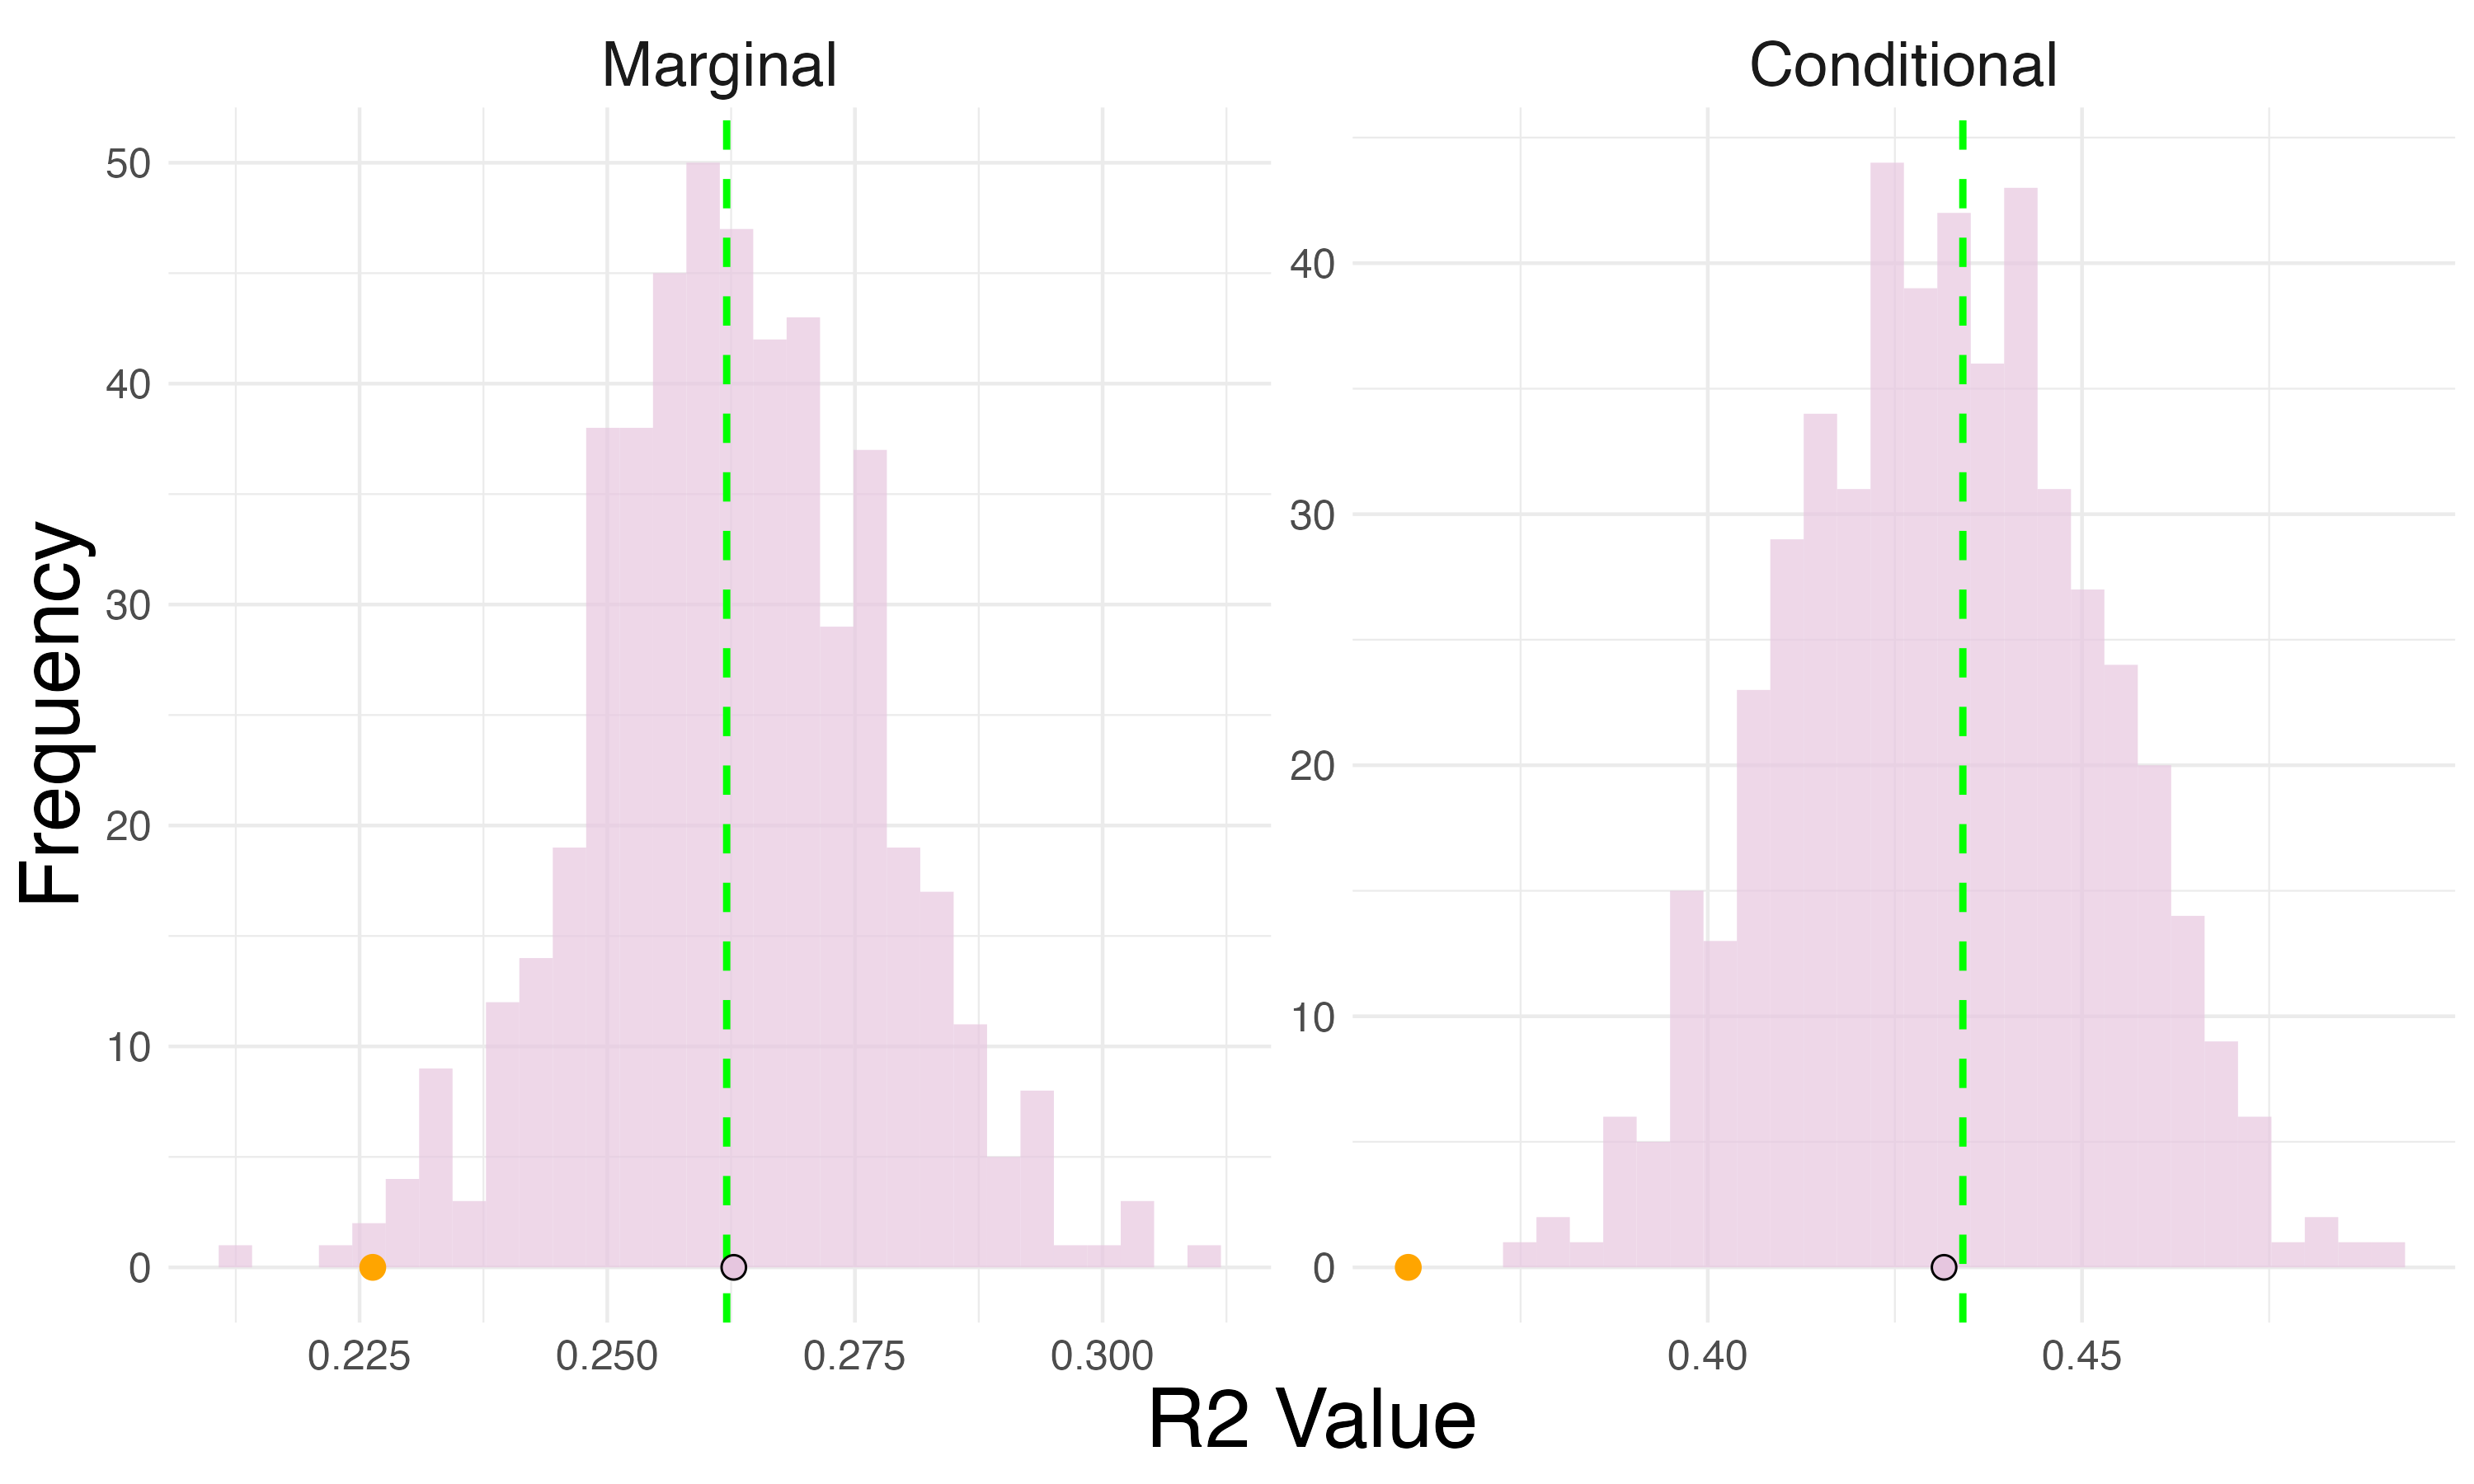
\includegraphics[width=1\linewidth]{Figures/Simulation study/R2_logit_high_neg.png}
%   \caption{Histogram with the estimated marginal $R^2$ (left) and conditional $R^2$ (right) from the BVI method for the binomial regression for the different correlation levels $\rho$ across $N_{\text{sim}}=500$ simulations. The expected values are displayed as vertical green lines, and can be found in \Cref{table:r2values}. The mean value of the $R^2$ values for all simulations is marked with a circle at the bottom. (a) Marginal and conditional $R^2$ estimates for $\rho=-0.4$.}
%   \label{fig:r2_logit_high_neg}
% \end{figure}
% \begin{figure}[H]\ContinuedFloat
%   \centering
%   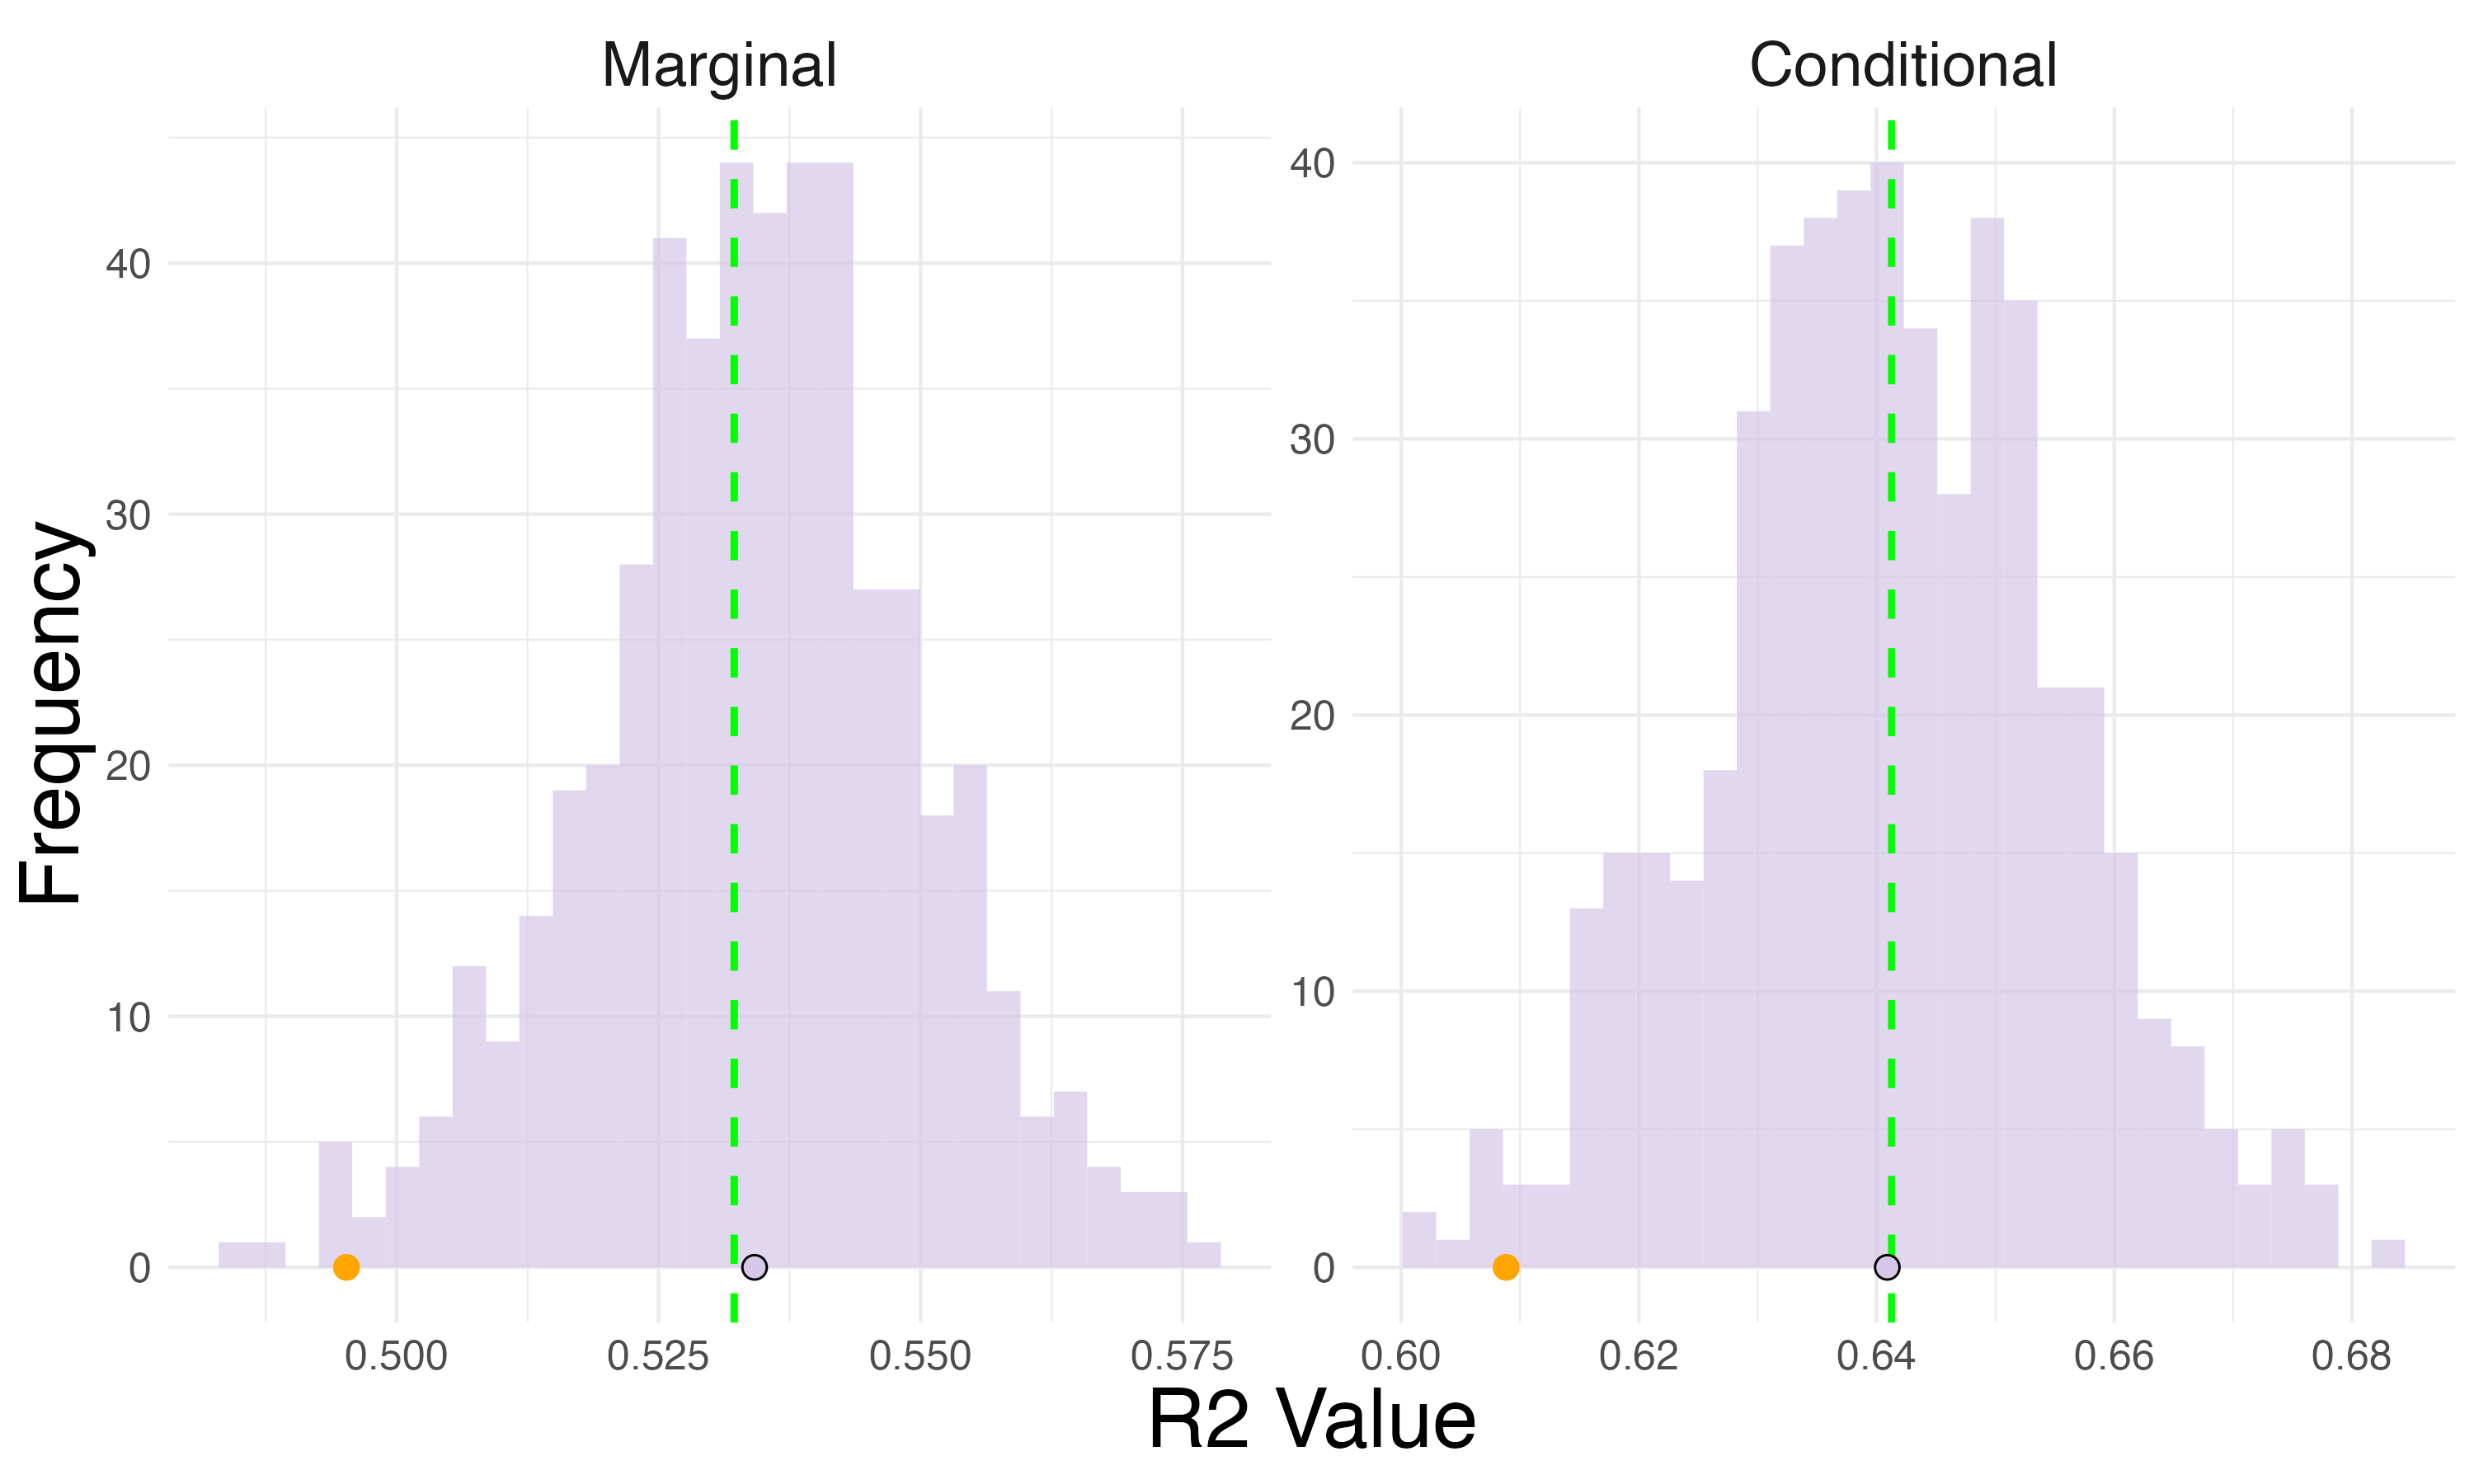
\includegraphics[width=1\linewidth]{Figures/Simulation study/R2_logit_low_neg.png}
%   \caption{(b) Marginal and conditional $R^2$ estimates for $\rho=-0.1$.}
%   \label{fig:r2_logit_low_neg}
% \end{figure}
% \begin{figure}[H]\ContinuedFloat
%   \centering
%   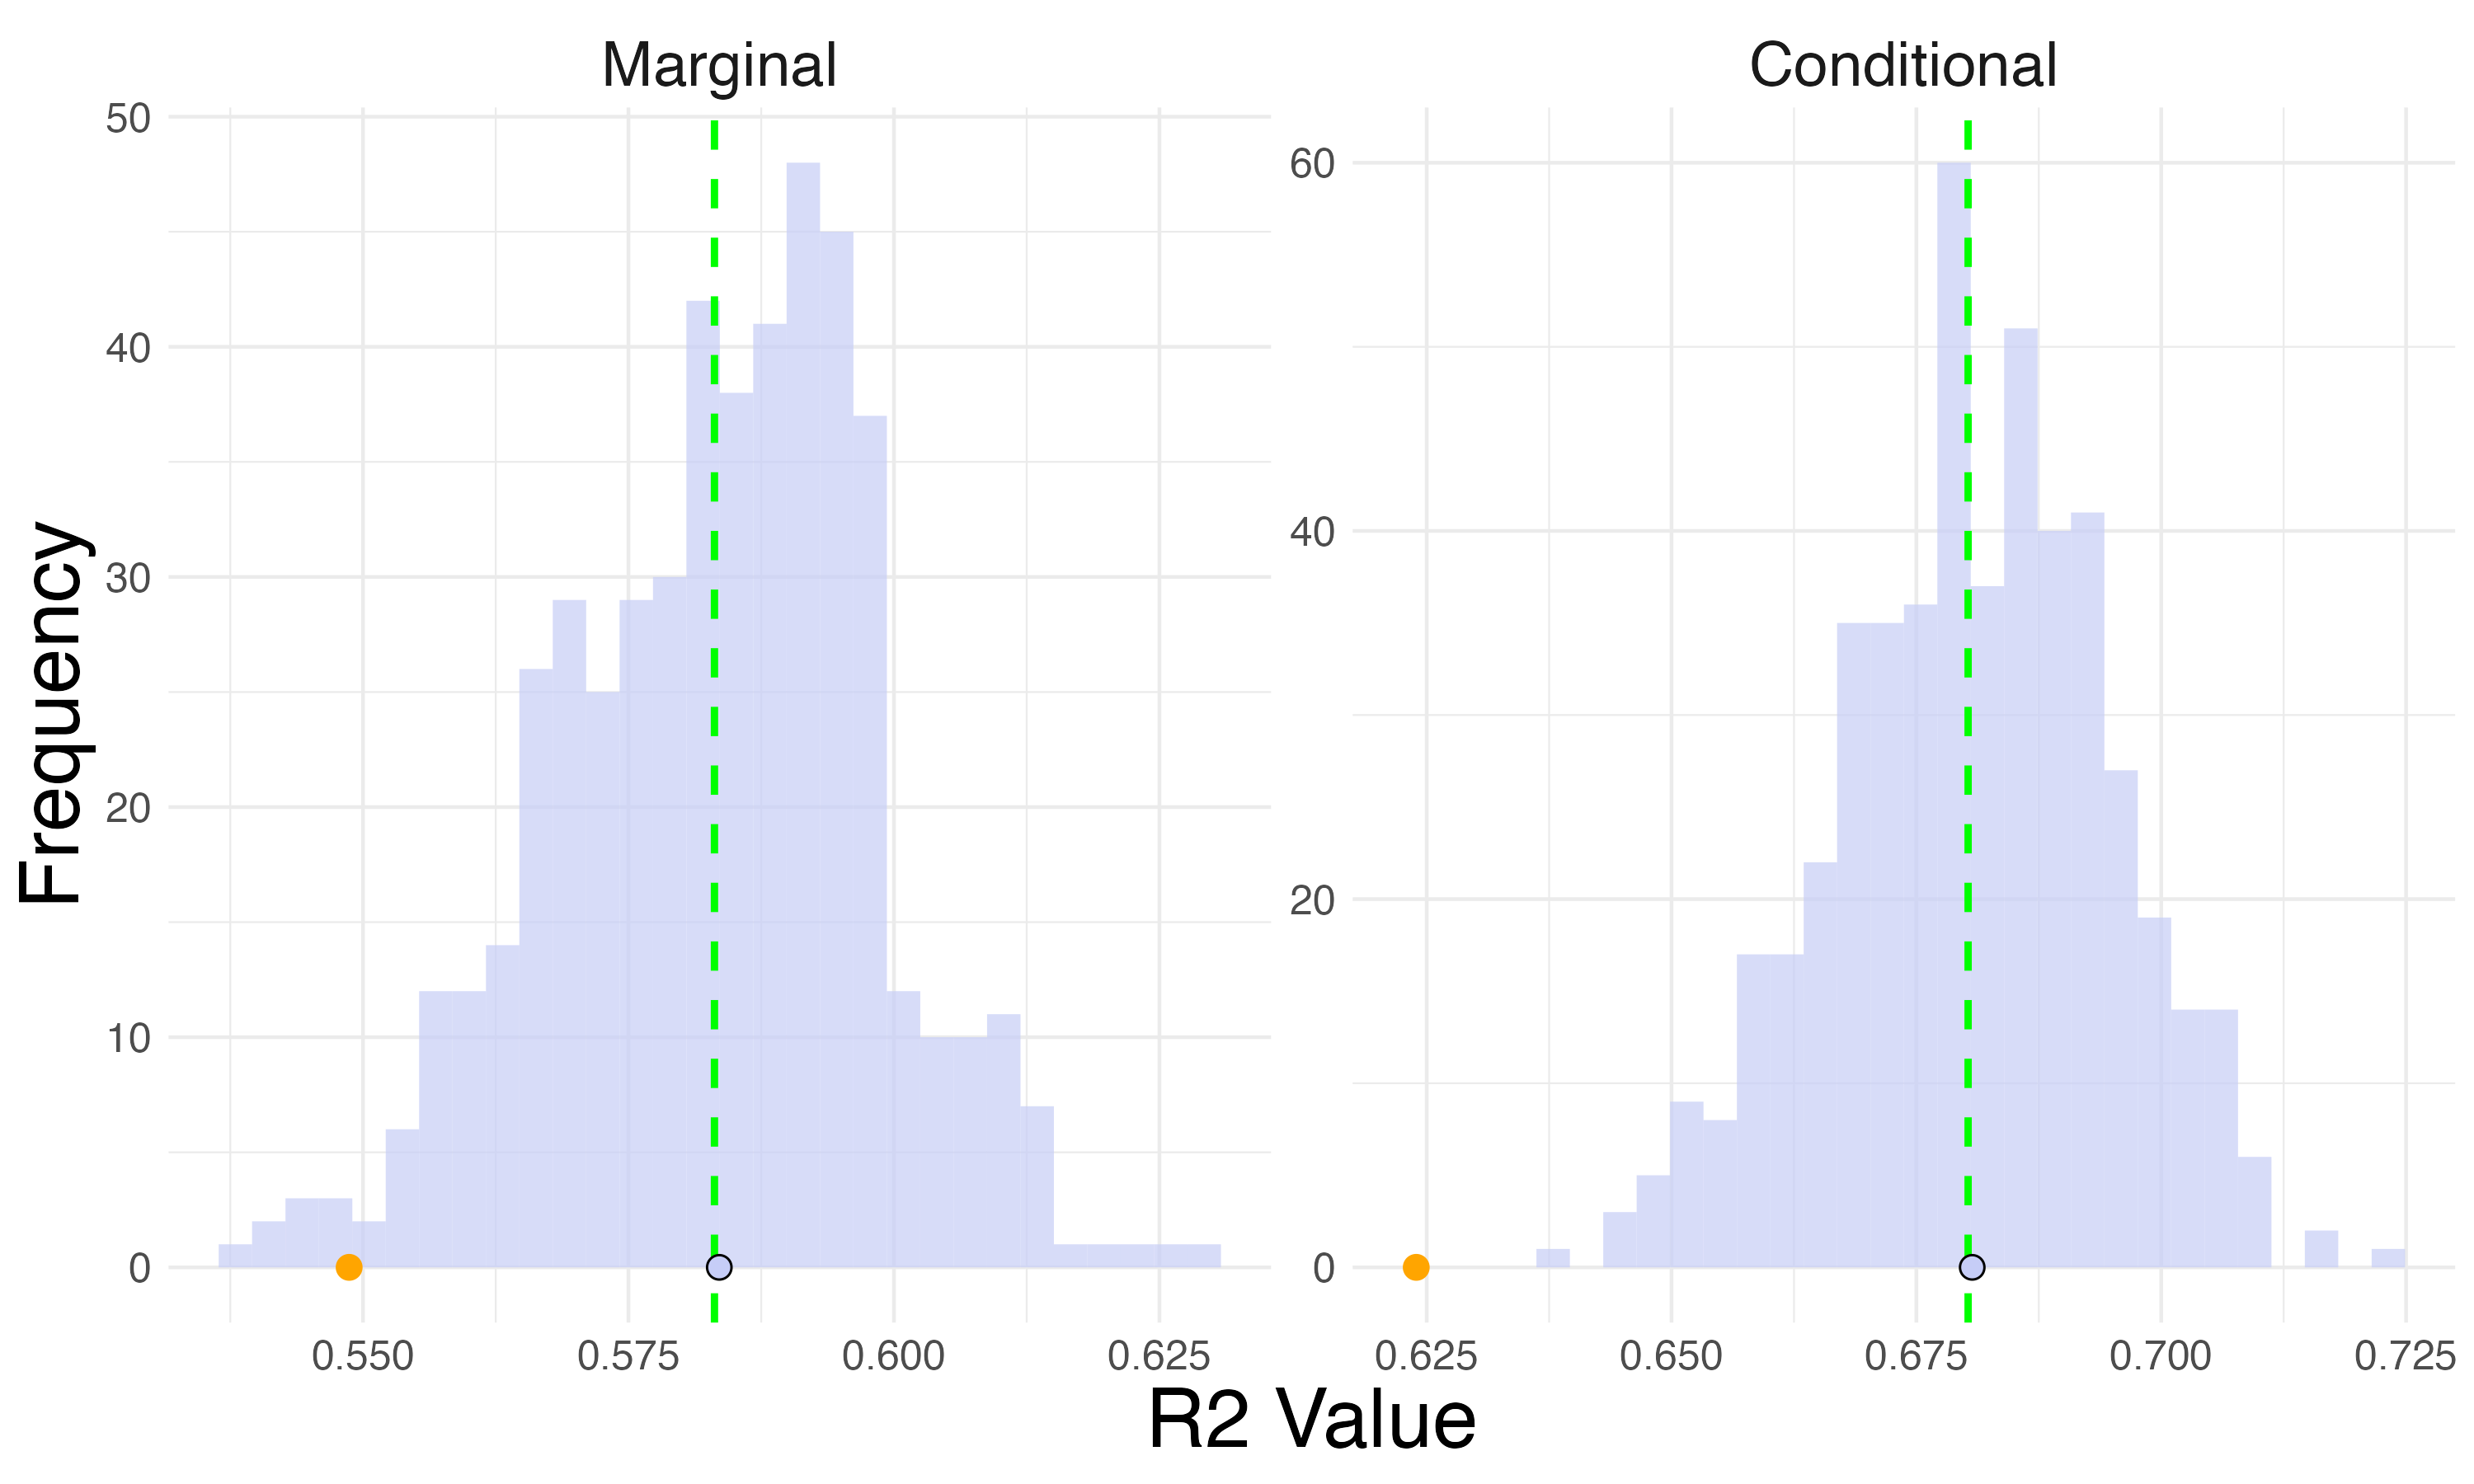
\includegraphics[width=1\linewidth]{Figures/Simulation study/R2_logit_no.png}
%   \caption{(c) Marginal and conditional $R^2$ estimates for $\rho=0$.}
%   \label{fig:r2_logit_no}
% \end{figure}
% \begin{figure}[H]\ContinuedFloat
%   \centering
%   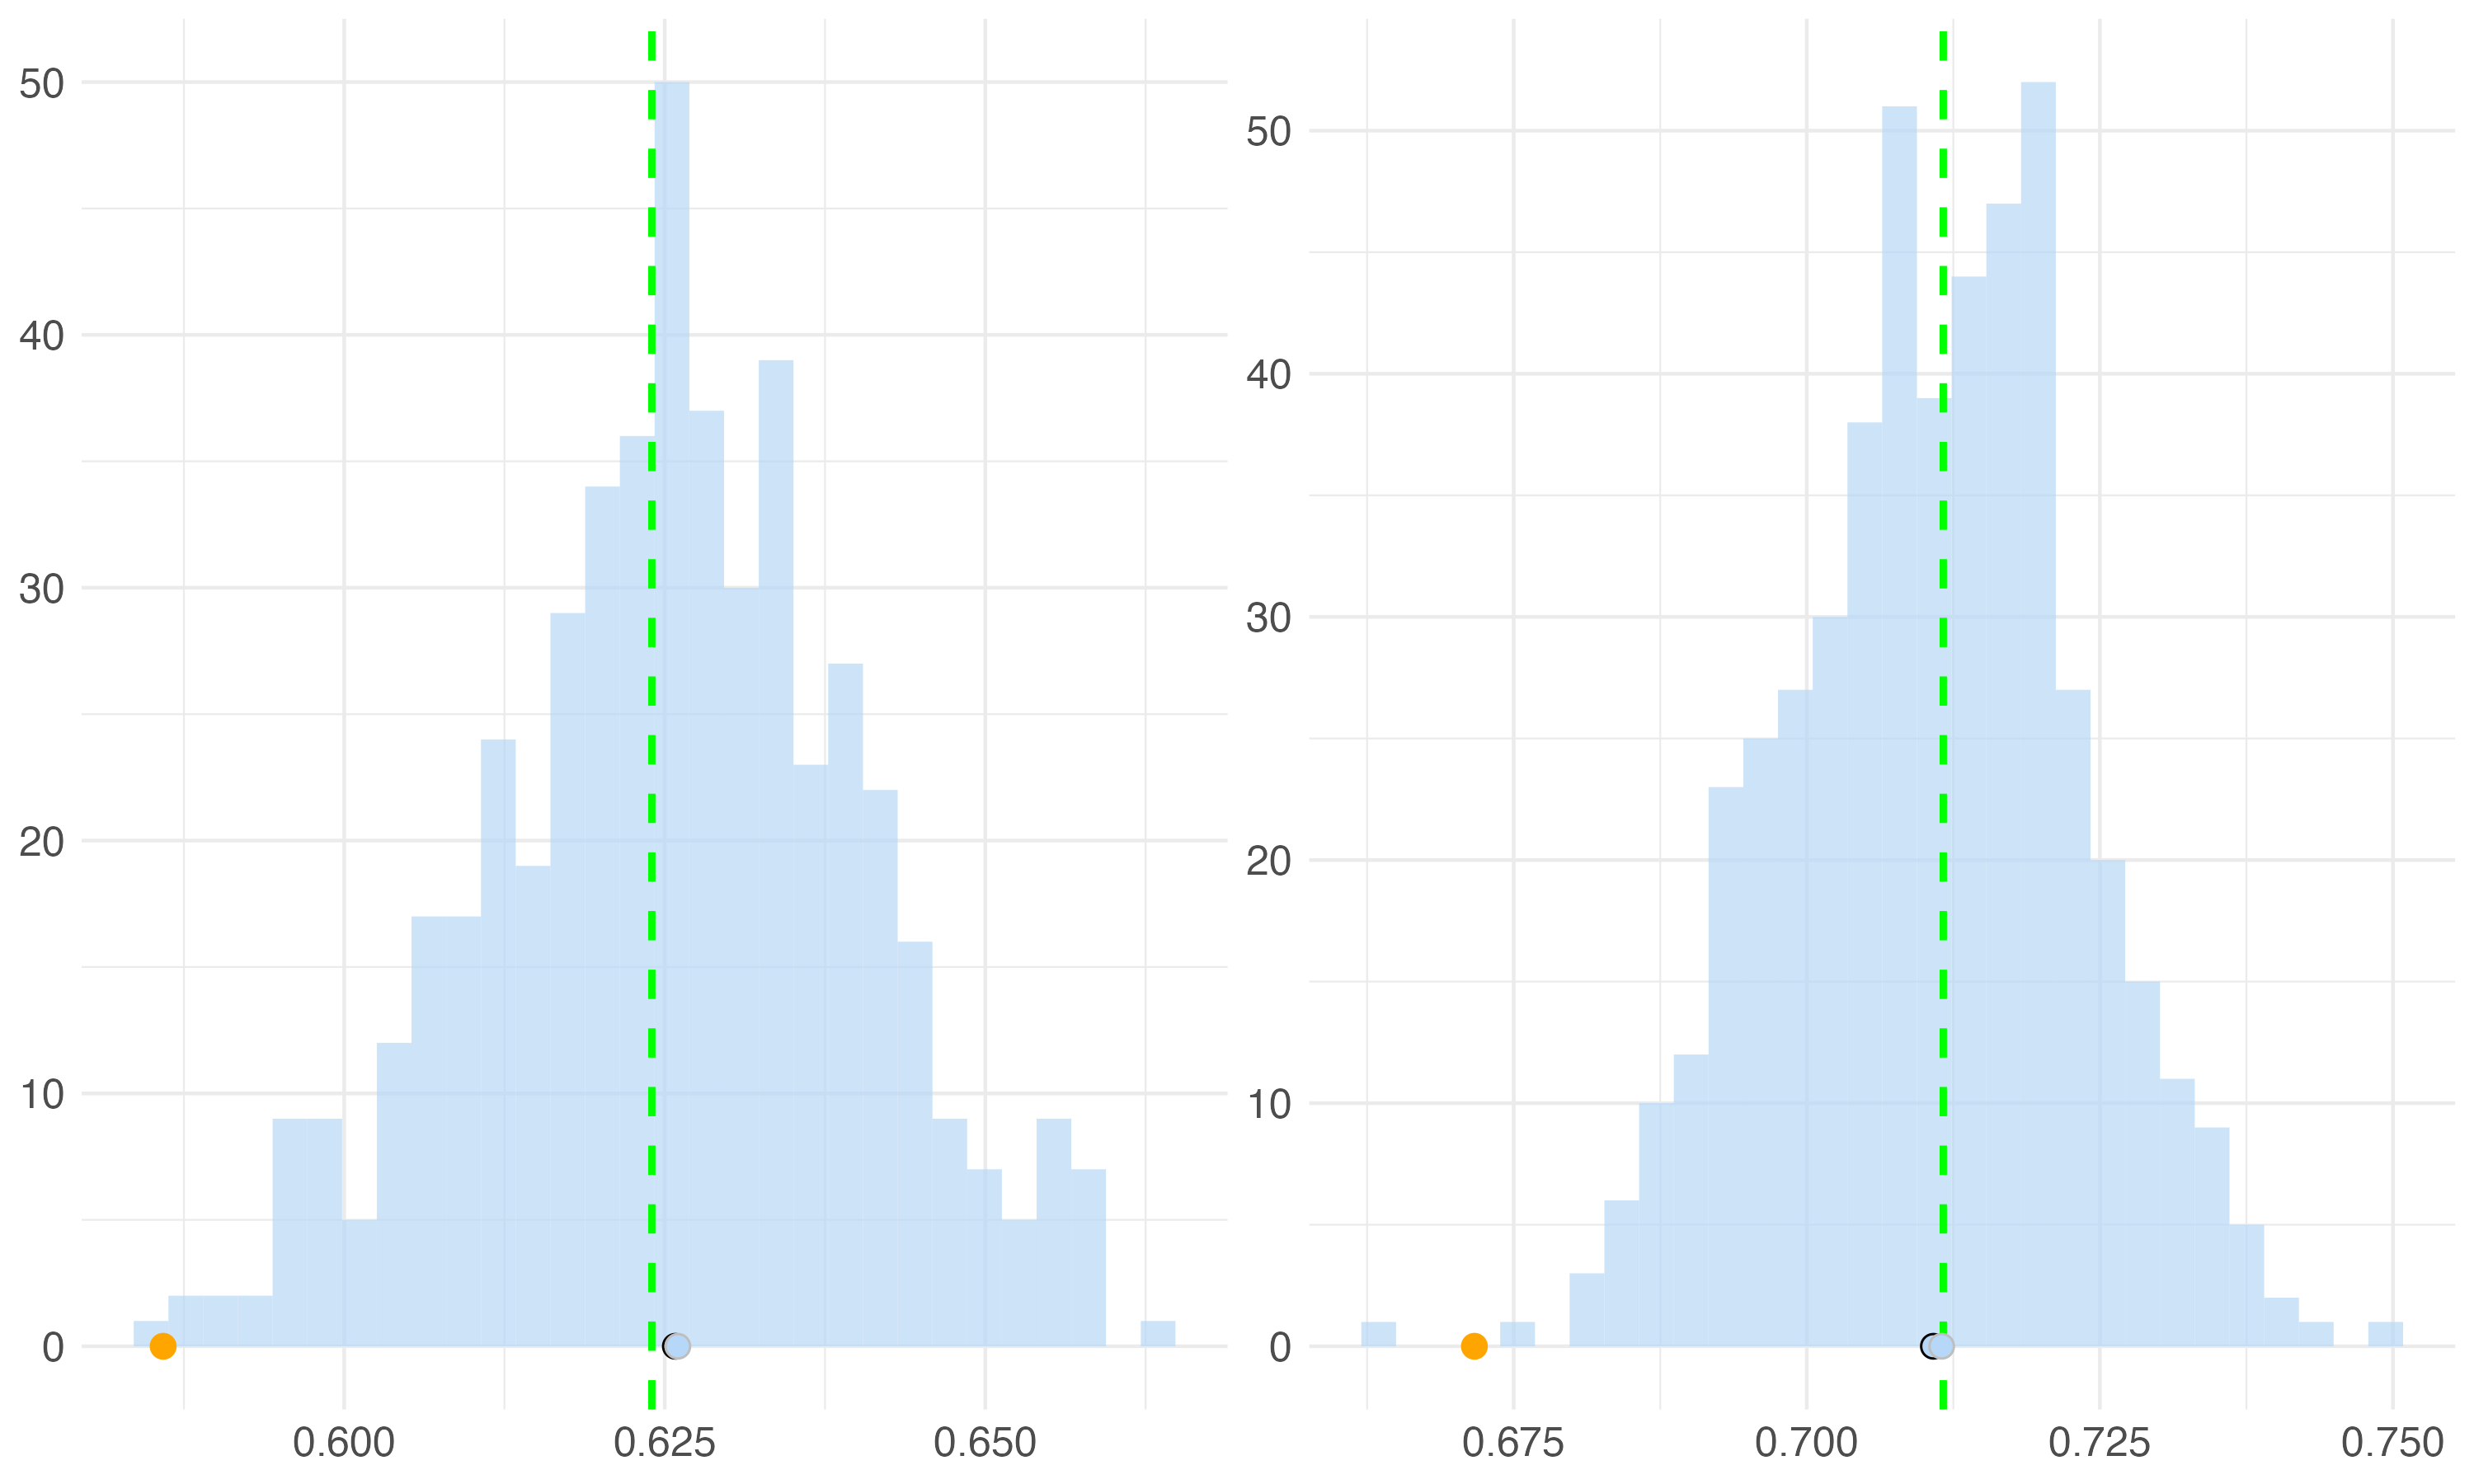
\includegraphics[width=1\linewidth]{Figures/Simulation study/R2_logit_low_pos.png}
%   \caption{(d) Marginal and conditional $R^2$ estimates for $\rho=0.1$.}
%   \label{fig:r2_logit_low_pos}
% \end{figure}
% \begin{figure}[H]\ContinuedFloat
%   \centering
%   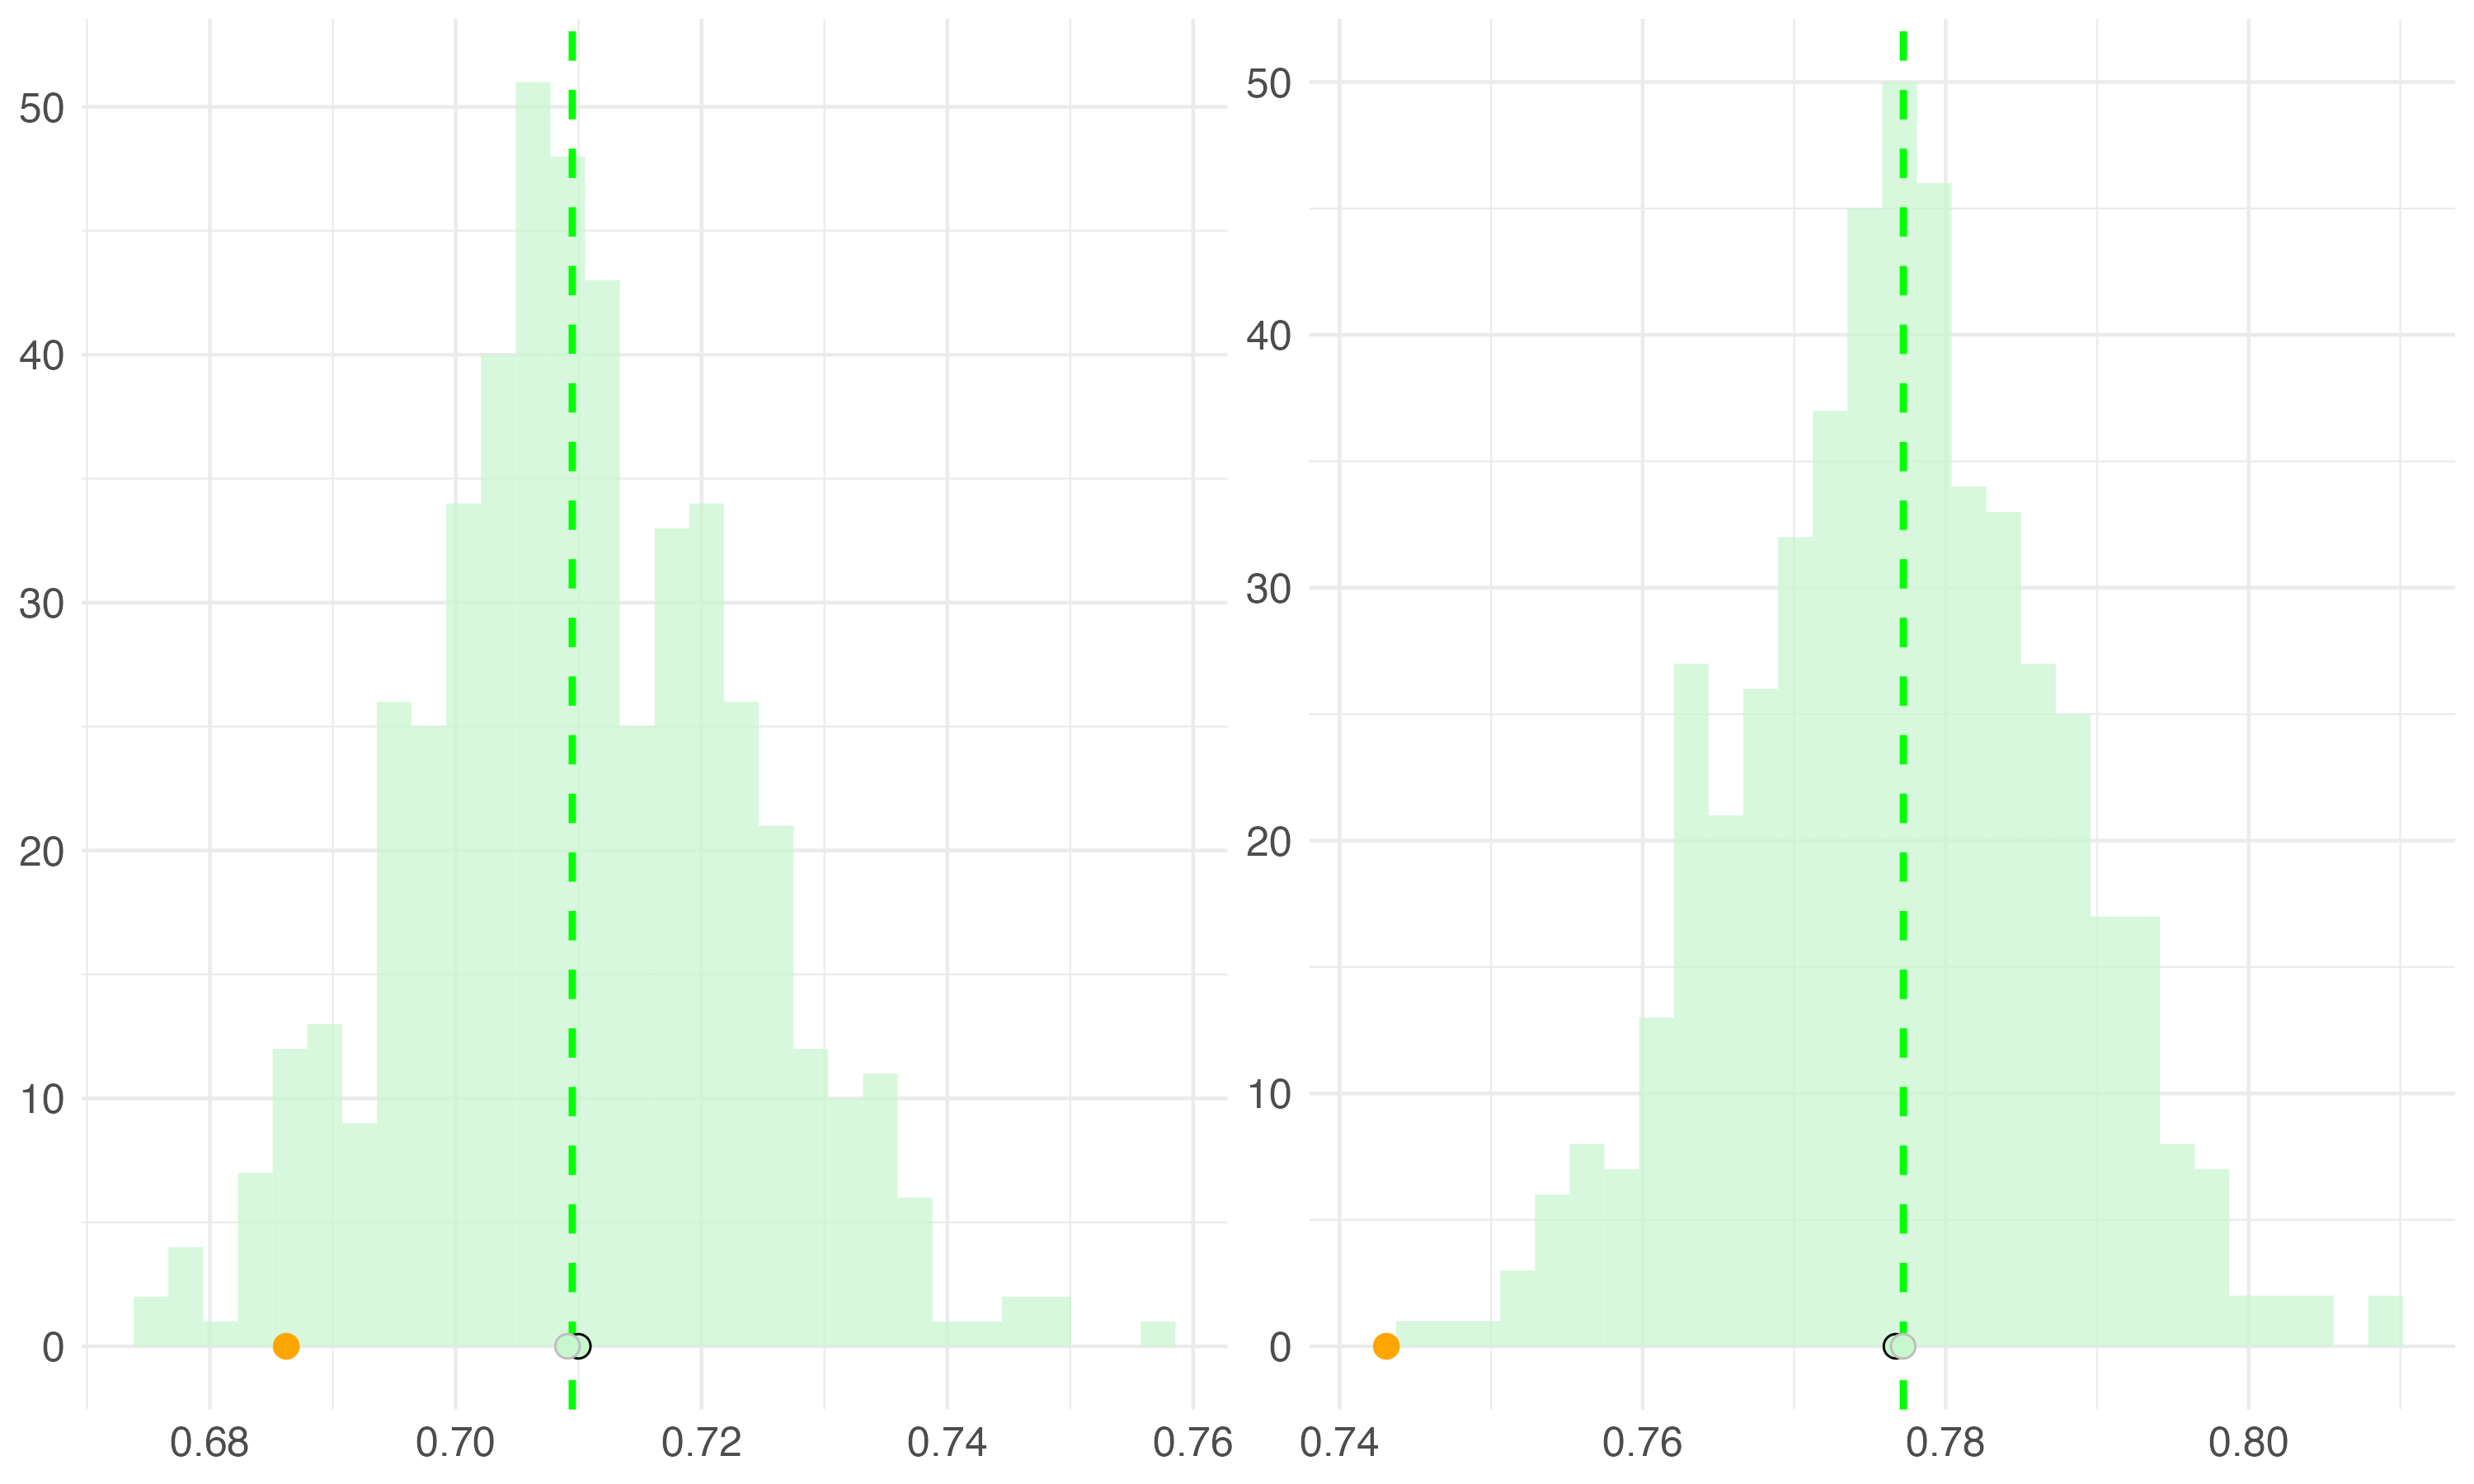
\includegraphics[width=1\linewidth]{Figures/Simulation study/R2_logit_high_pos.png}
%   \caption{(e) Marginal and conditional $R^2$ estimates for $\rho=0.4$.}
%   \label{fig:r2_logit_high_pos}
% \end{figure}
\begin{figure}[H]
  \centering
  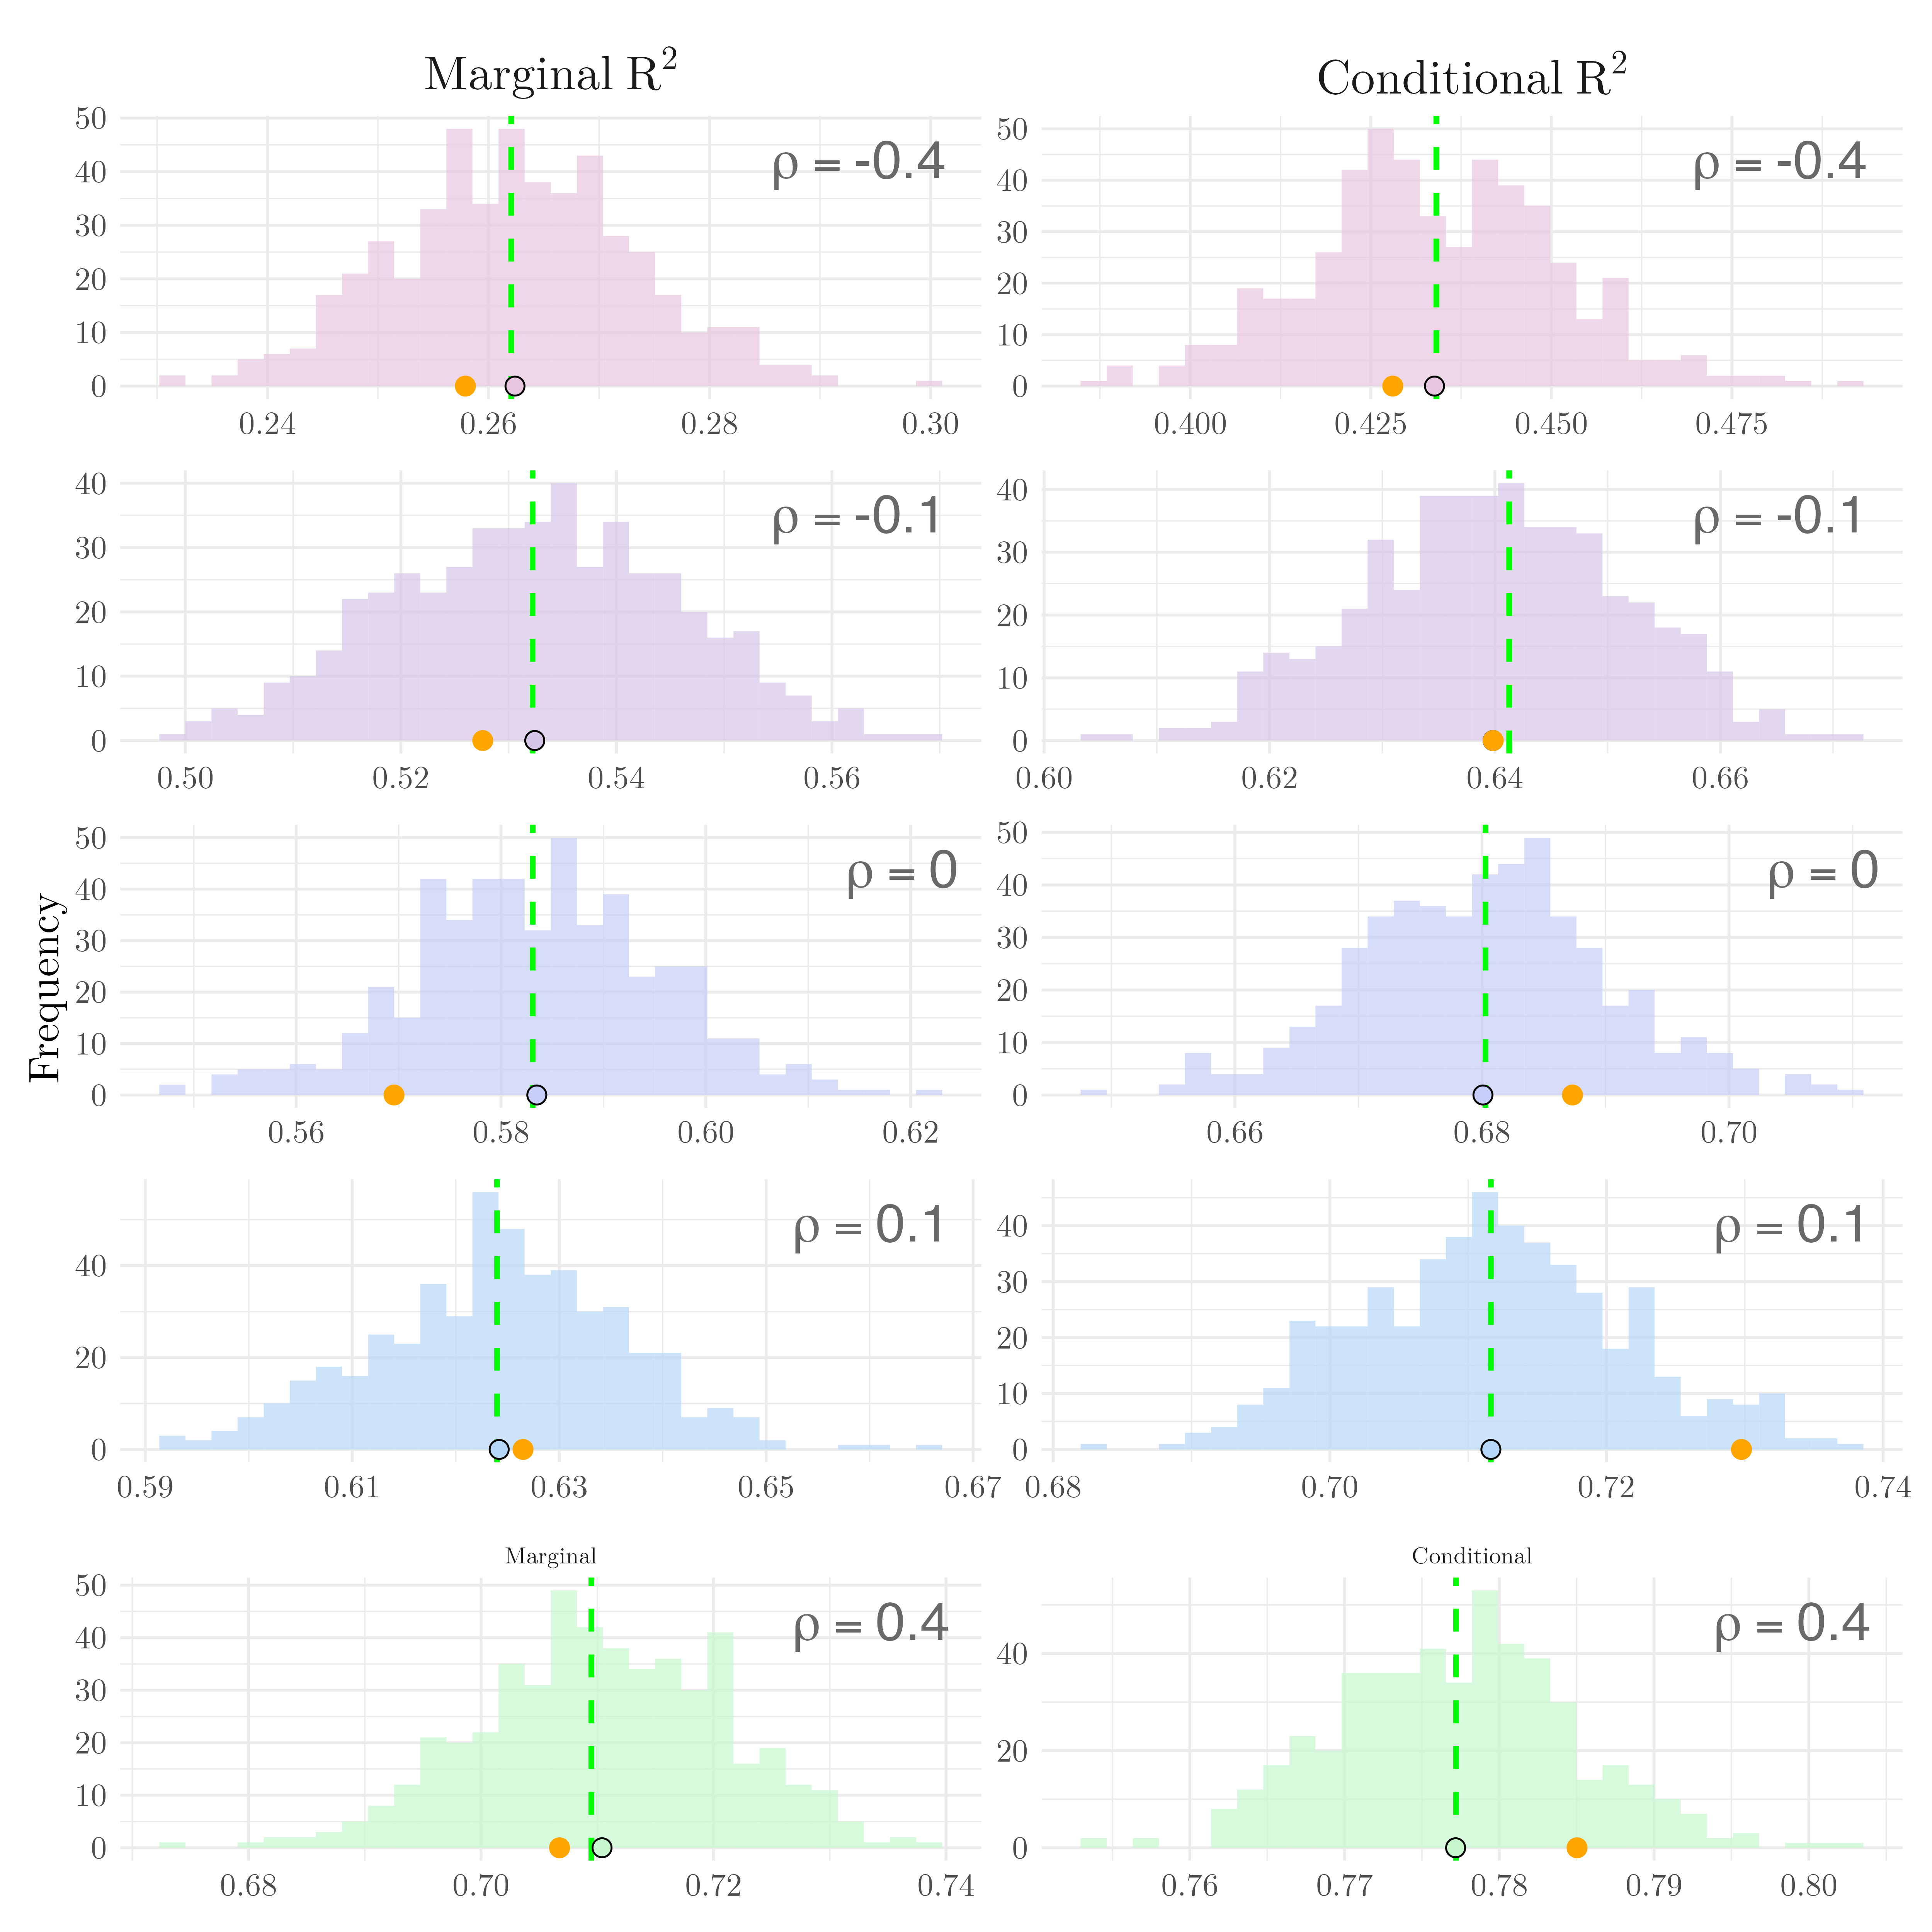
\includegraphics[width=1.1\linewidth]{Figures/Simulation study/R2_combined_logit.png}
  \caption{Histograms with the estimated marginal $R^2$ (left) and conditional $R^2$ (right) from the BVI method for the binomial regression for the different correlation levels $\rho=-0.4$ (top), $\rho=-0.1$ (second from the top), $\rho=0$ (middle), $\rho=0.1$ (second from bottom) and $\rho=0.4$ (bottom). The values are calculated by the Bayesian Variable Importance method from the $N_{\text{sim}}=500$ simulations in the simulation study. The expected values are displayed as vertical green lines, and can be found in \Cref{table:r2values}, while the orange dot denotes the estimate from the \texttt{rptR} package. The mean value of the $R^2$ values for all simulations is marked with a circle at the bottom of each histogram.}
  \label{fig:r2_combined_logit}
\end{figure}





% \begin{figure}[H]
%     \centering
%       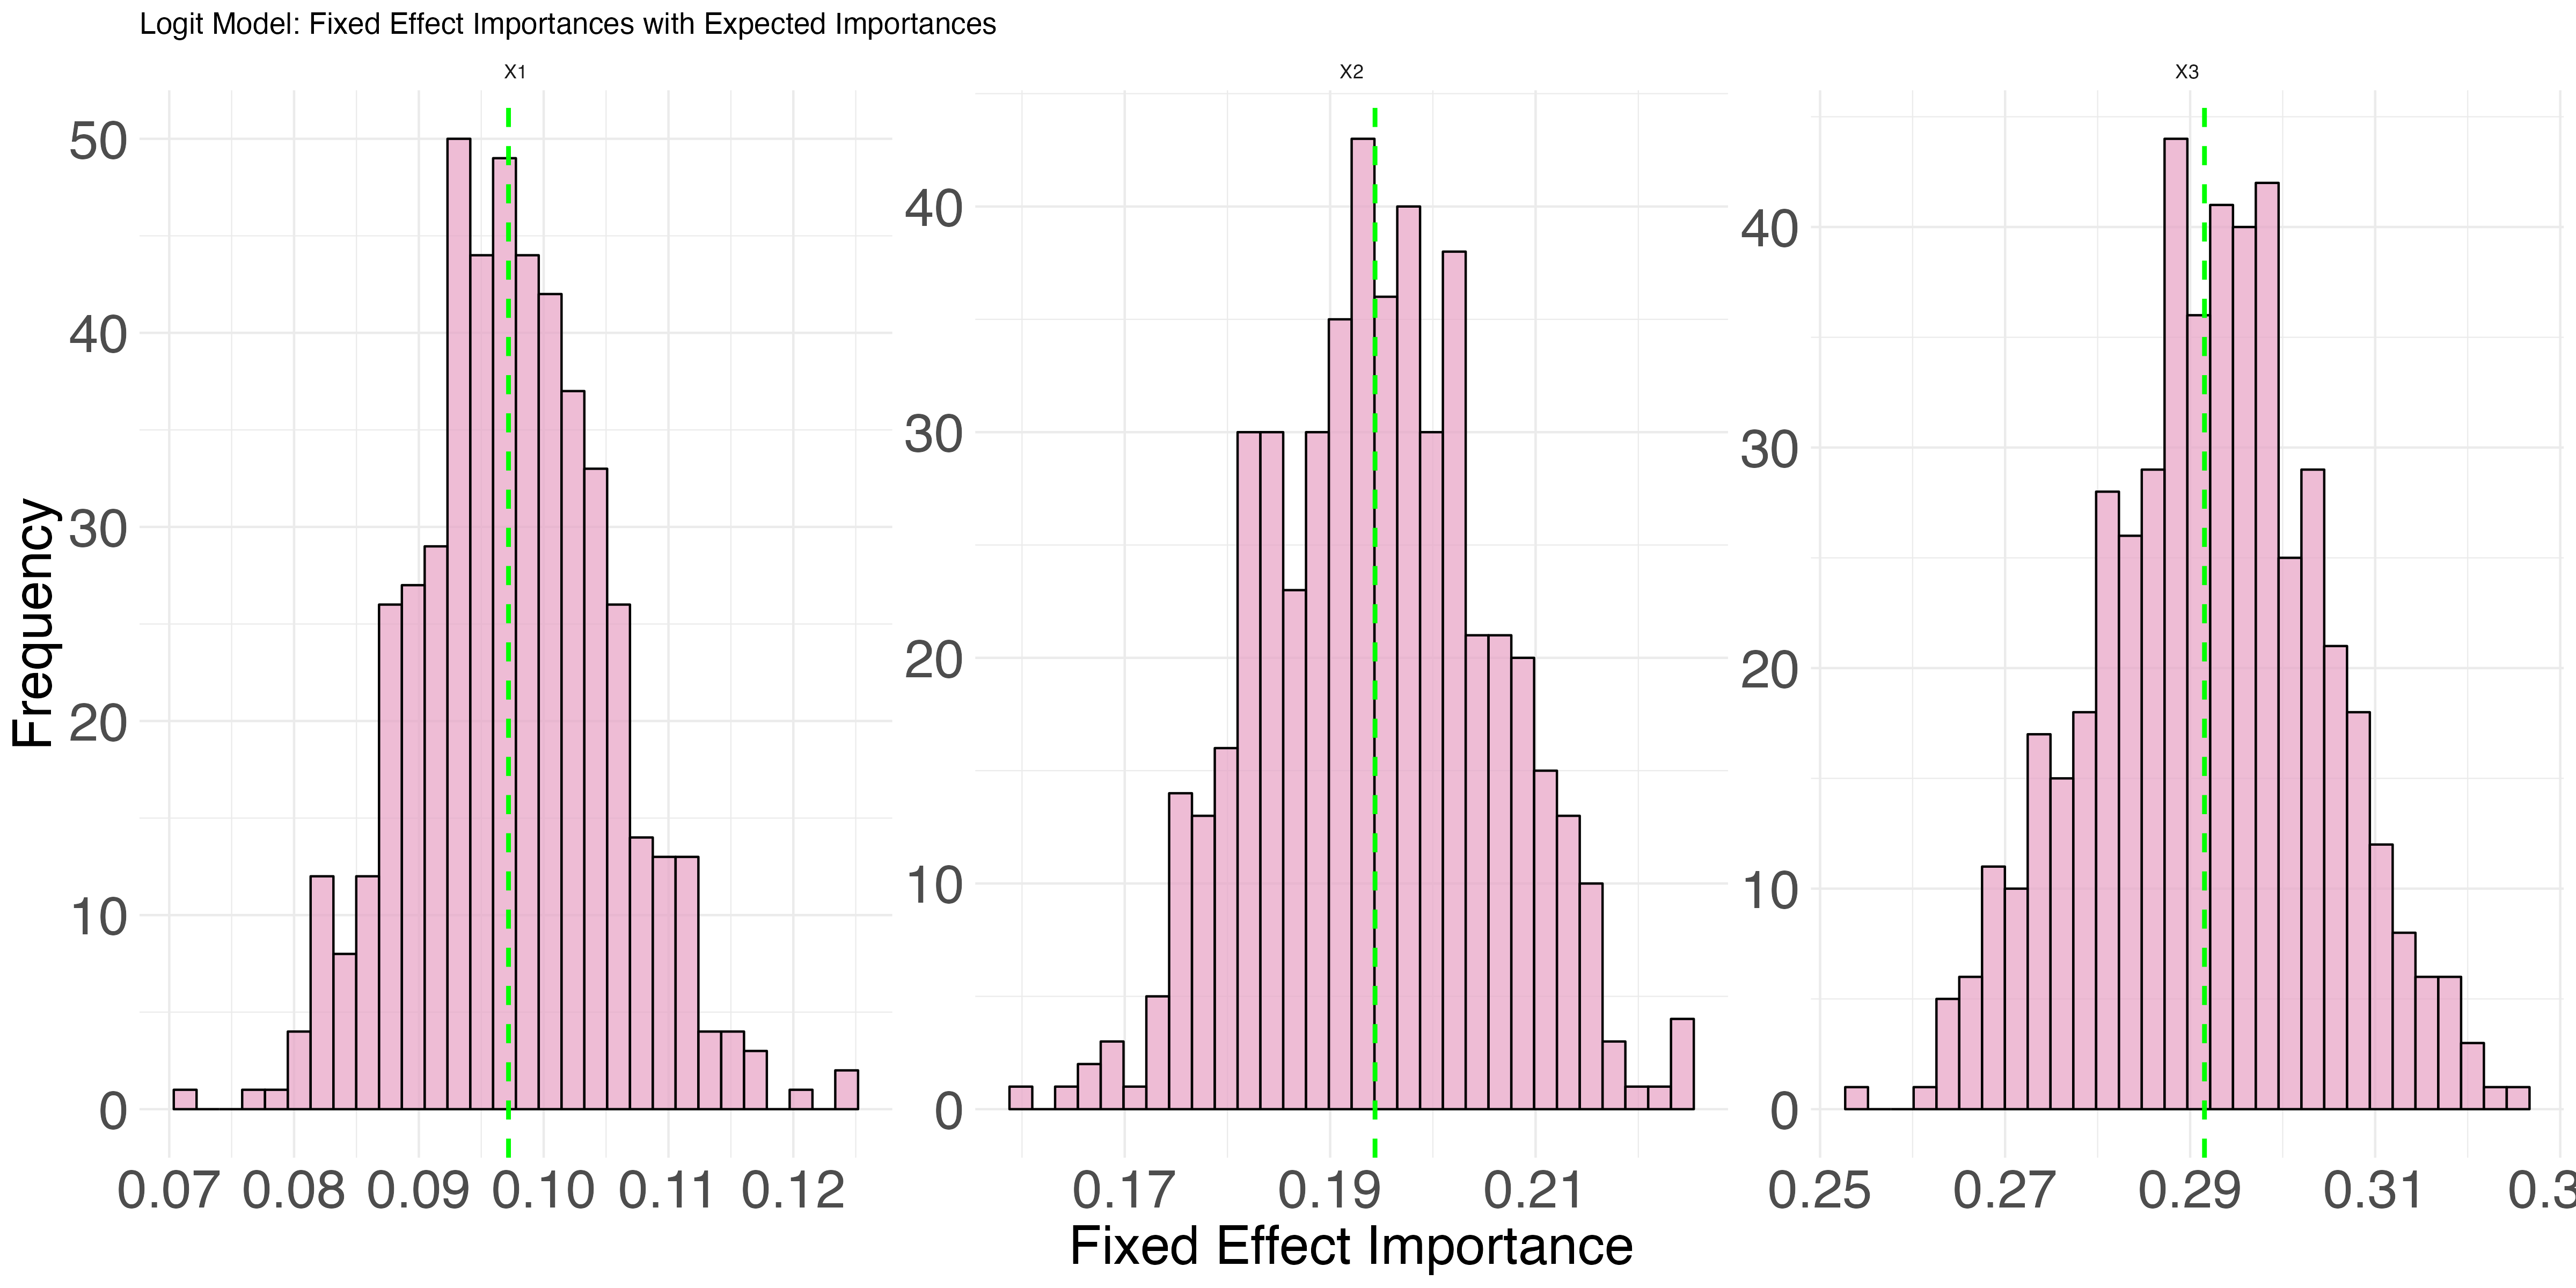
\includegraphics[width=1\linewidth]{Figures/Simulation study/Fixed_logit.png}
%       \caption{Relative importance of fixed effects for binomial GLMM with logit link. Blue line is expected importance}
%       \label{fig:relimp_binomial_logit_fixed}
%   \end{figure}
%   \begin{figure}[H]\ContinuedFloat
%     \centering
%     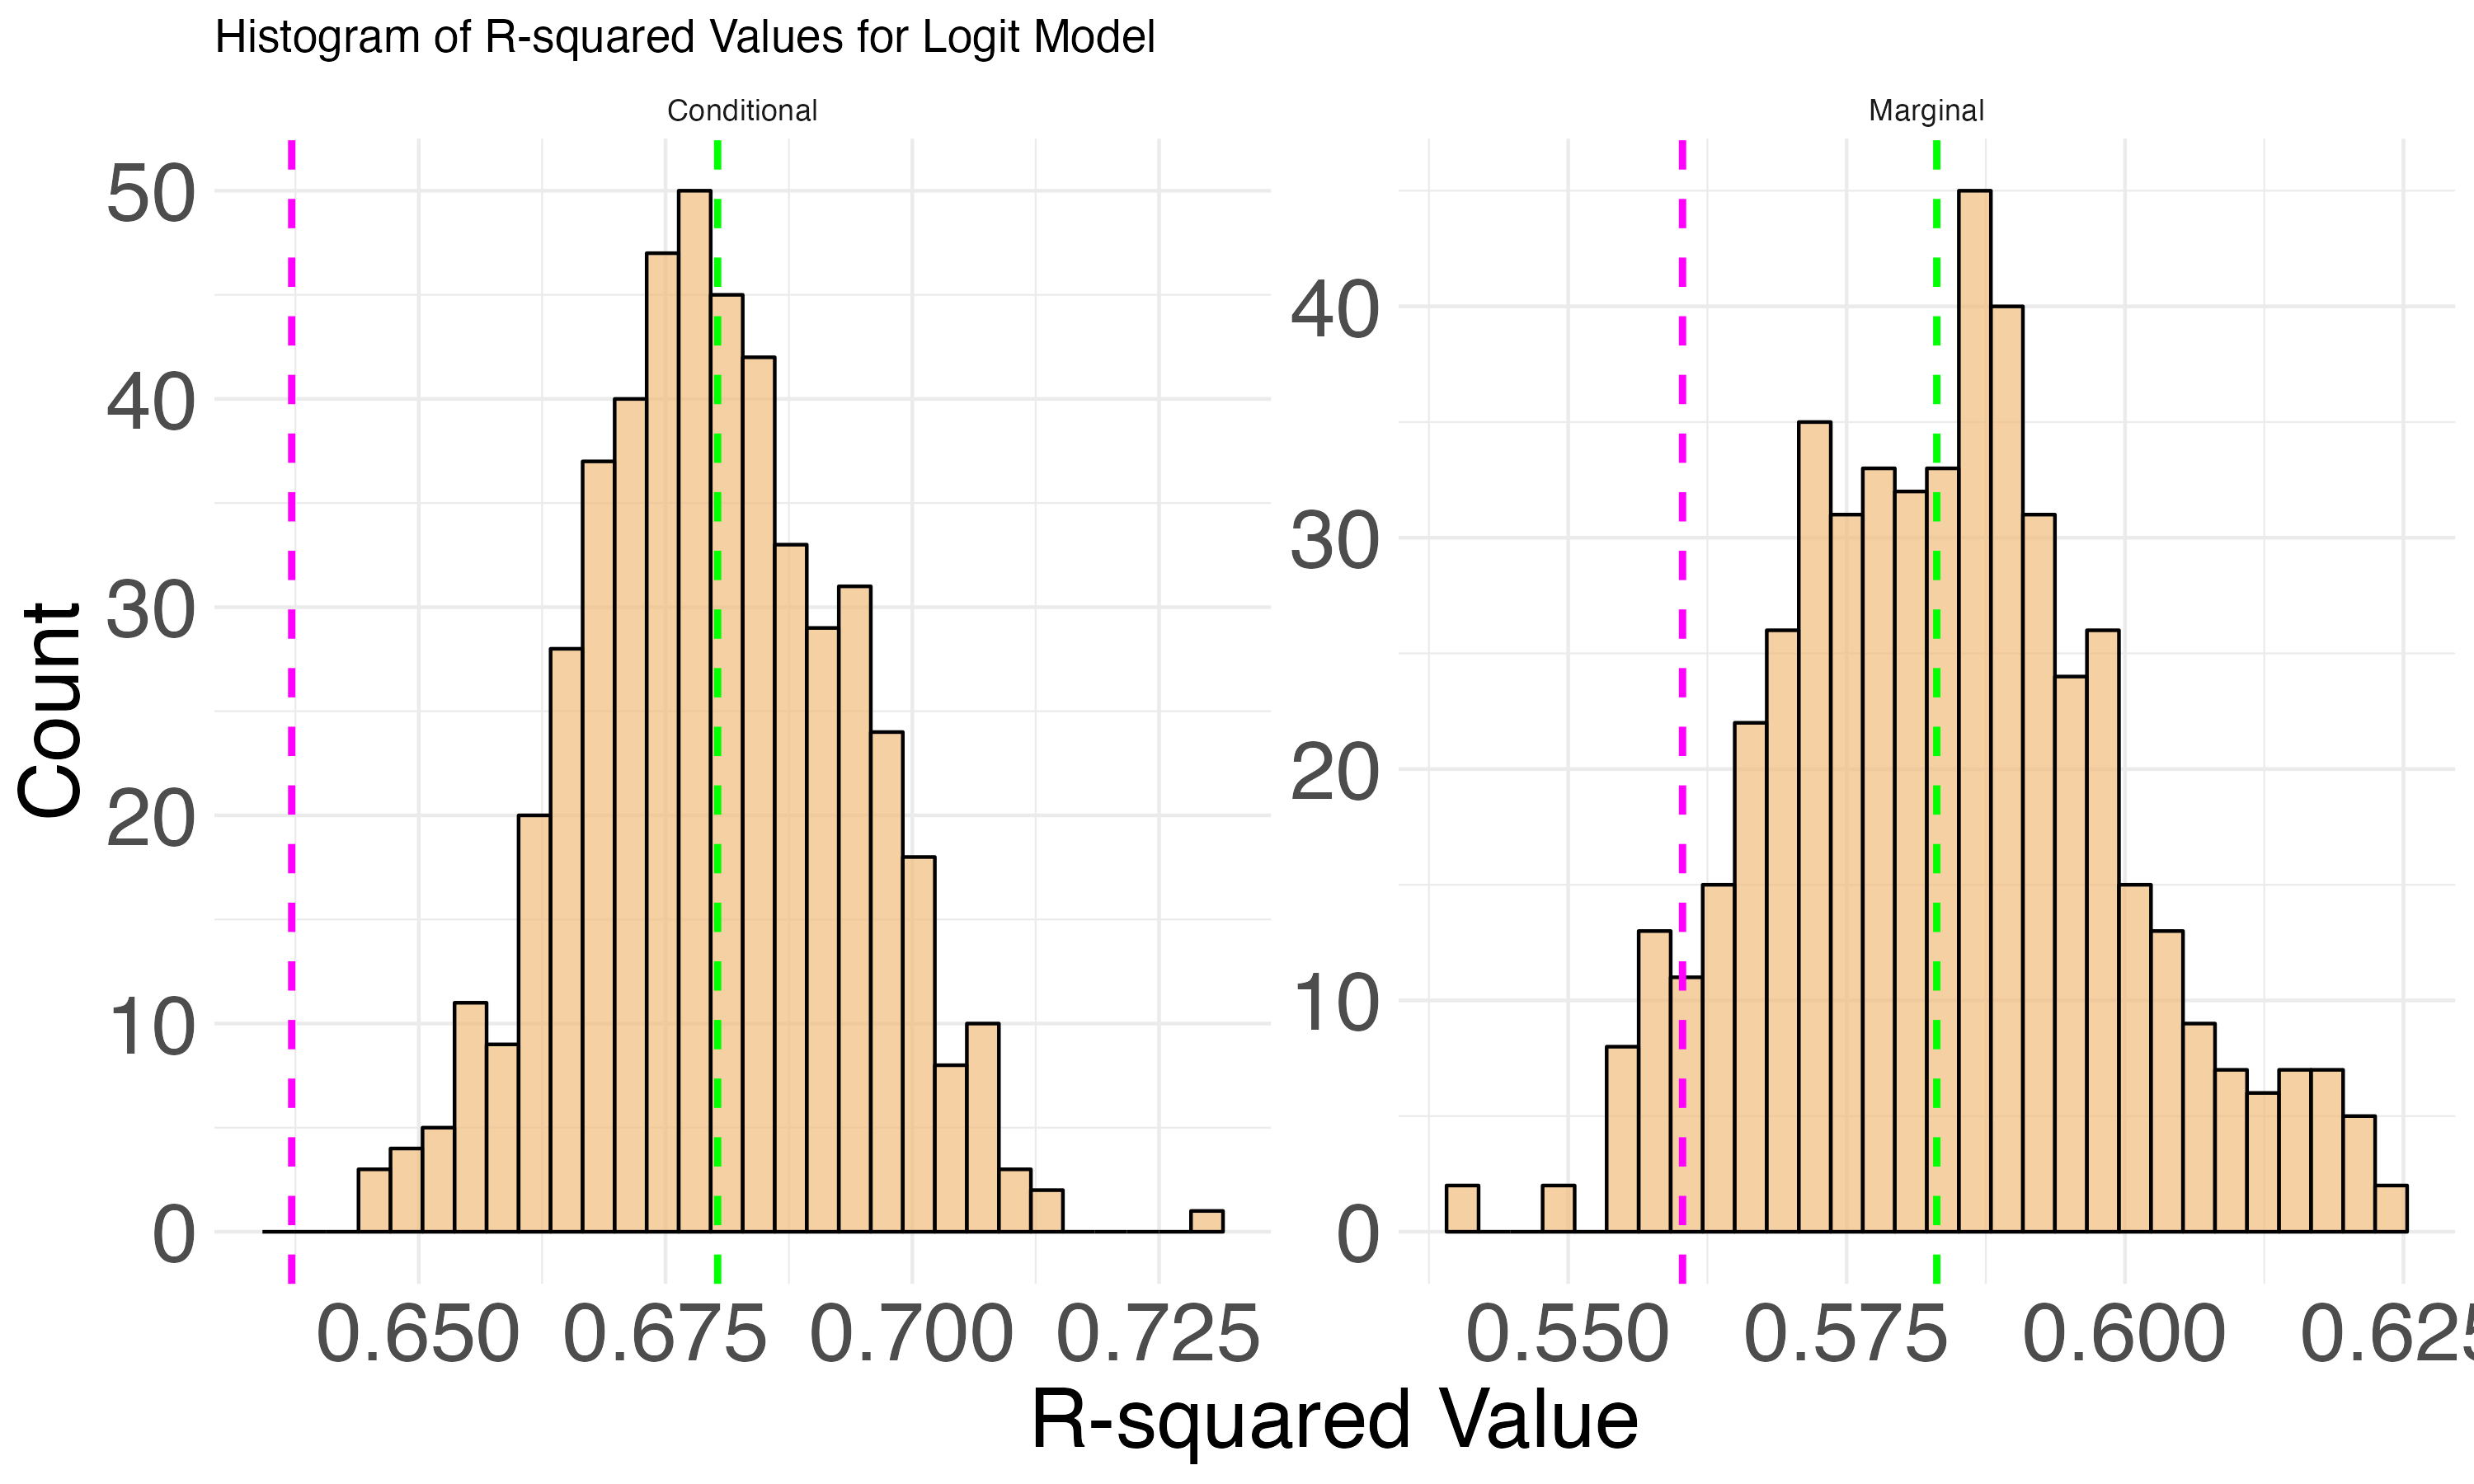
\includegraphics[width=1\linewidth]{Figures/Simulation study/R2_logit.png}
%     \caption{Conditional and marginal $R^2$ for binomial GLMM with logit link. The magenta line is Stoffel, green line is expected importance}
%       \label{fig:relimp_binomial_logit_r2}
%   \end{figure}

  % \begin{figure}[H]
  %   \centering
  %     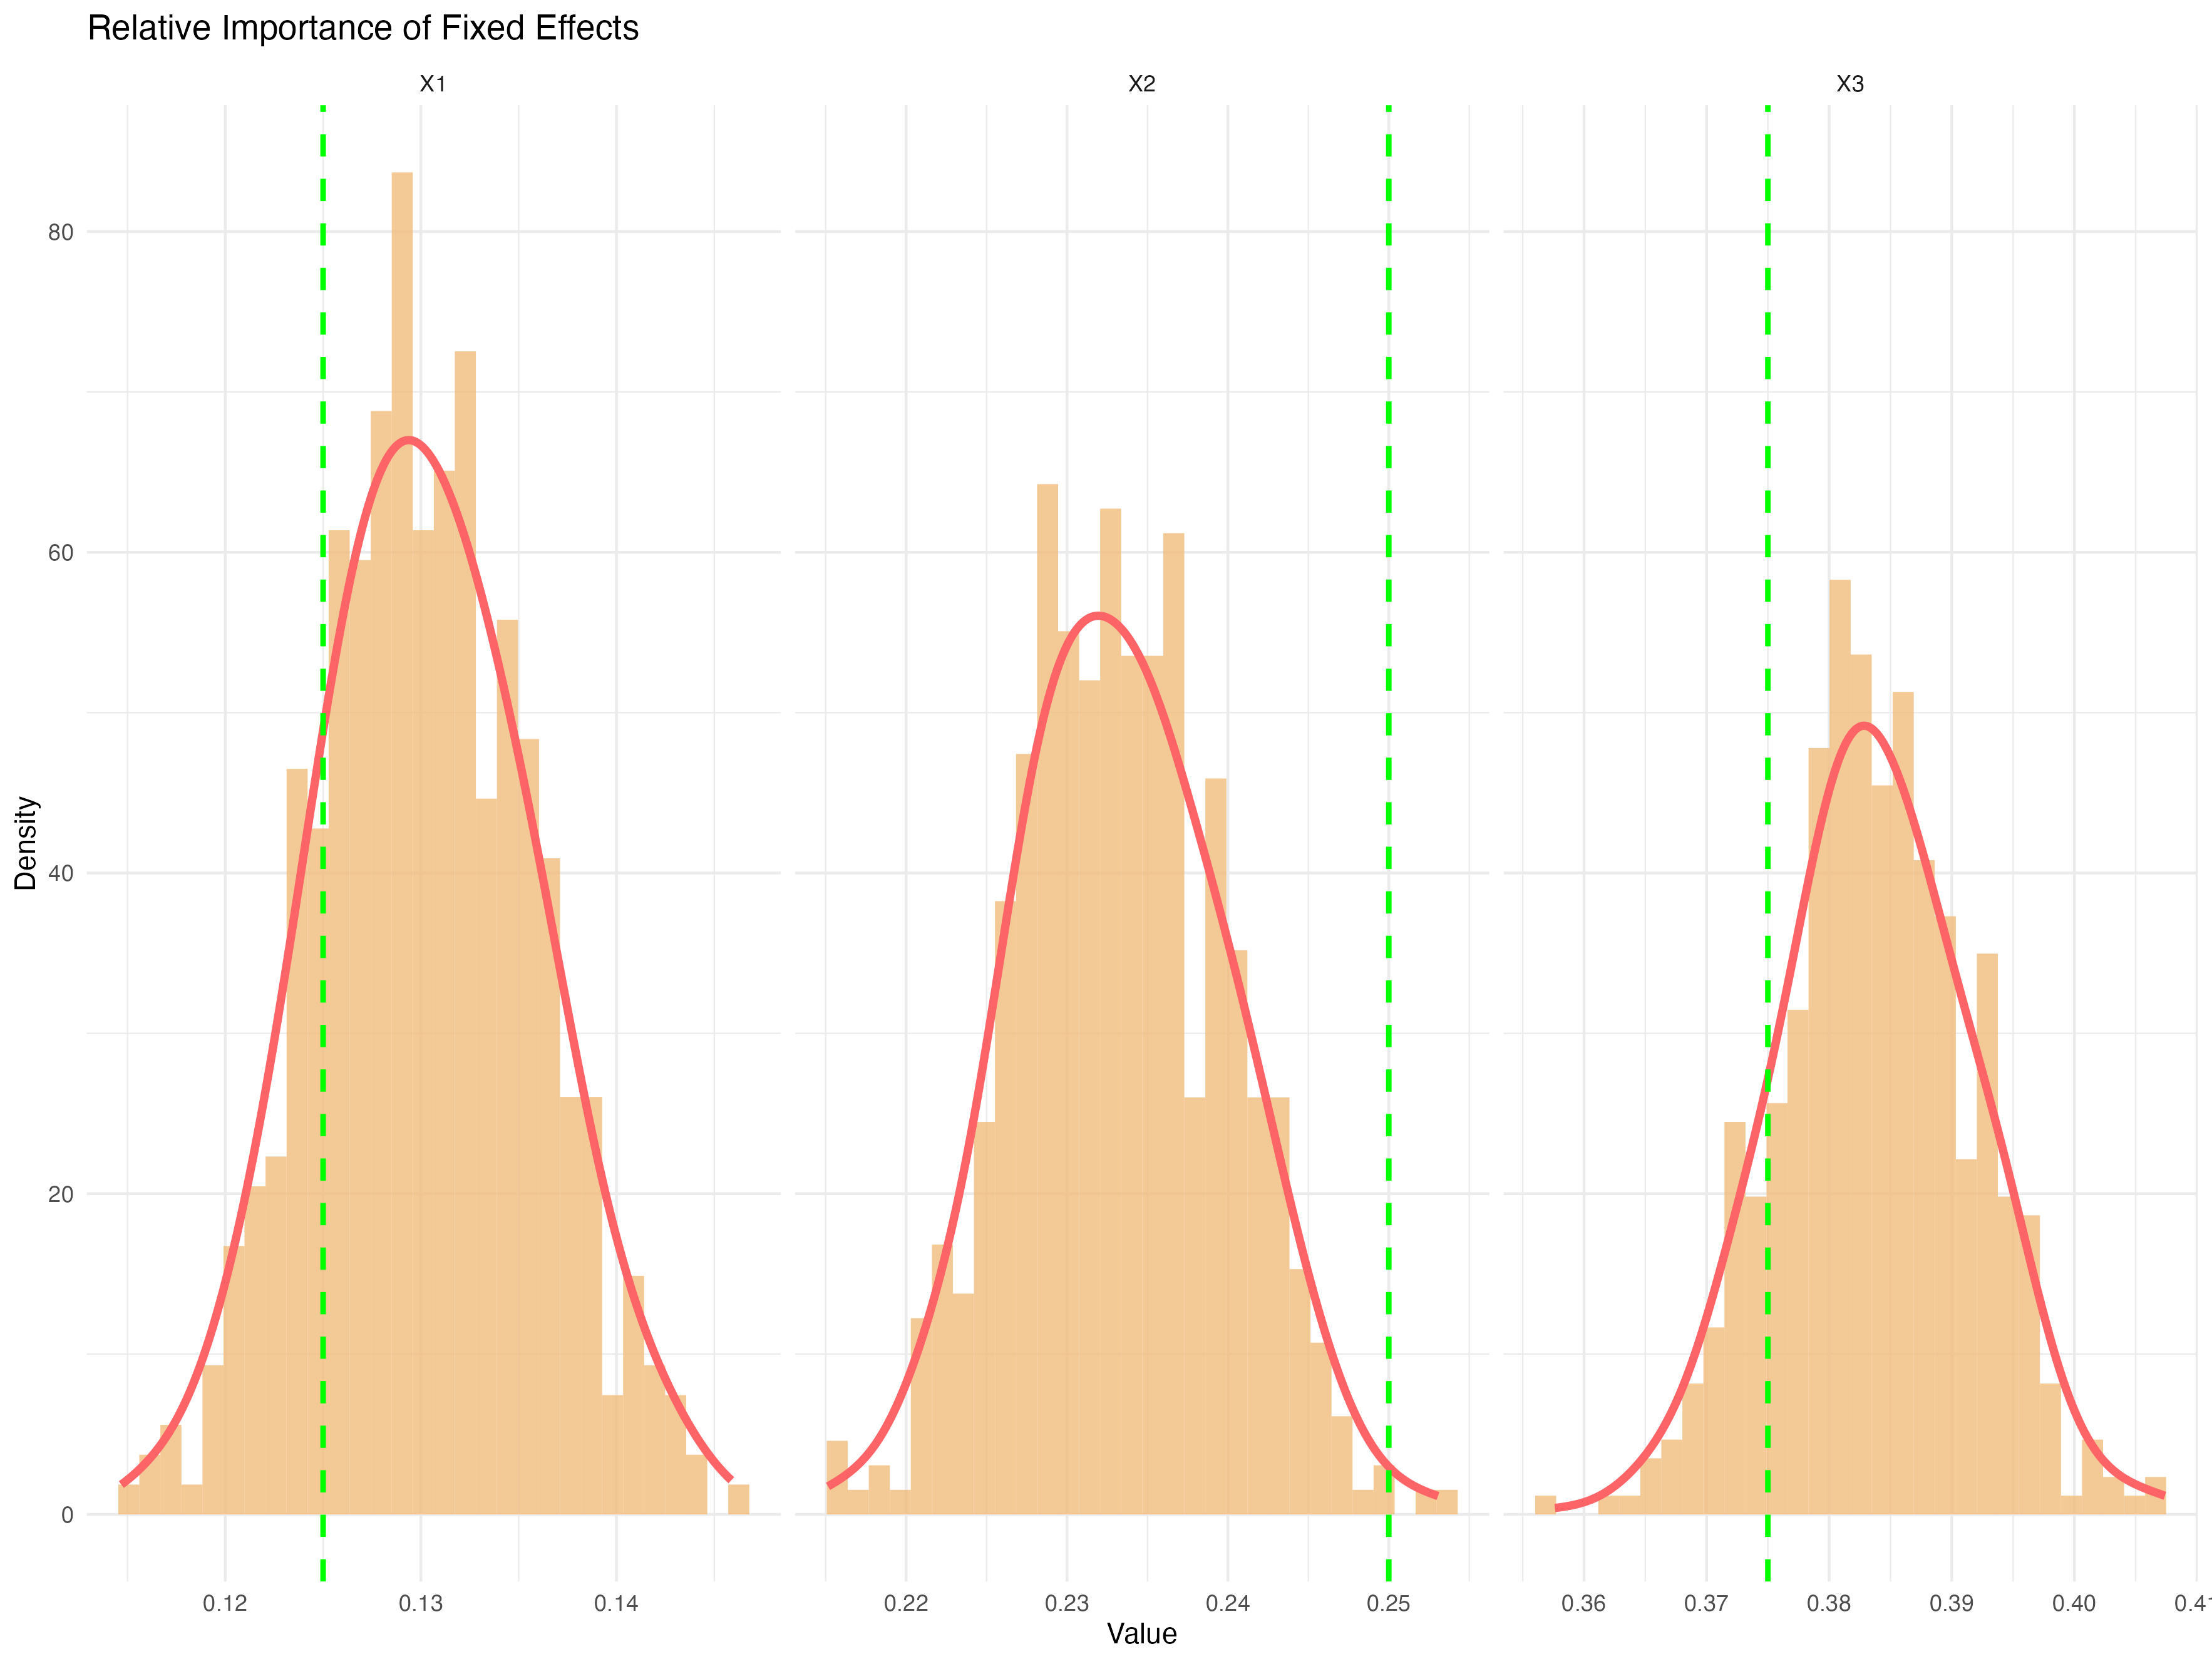
\includegraphics[width=0.7\linewidth]{Figures/Simulation study/Binomial_probit_fixed.png}
  %     \caption{Relative importance of fixed effects for binomial GLMM with probit link}
  %     \label{fig:relimp_binomial_probit_fixed}
  % \end{figure}
  % \begin{figure}[H]\ContinuedFloat
  %   \centering
  %   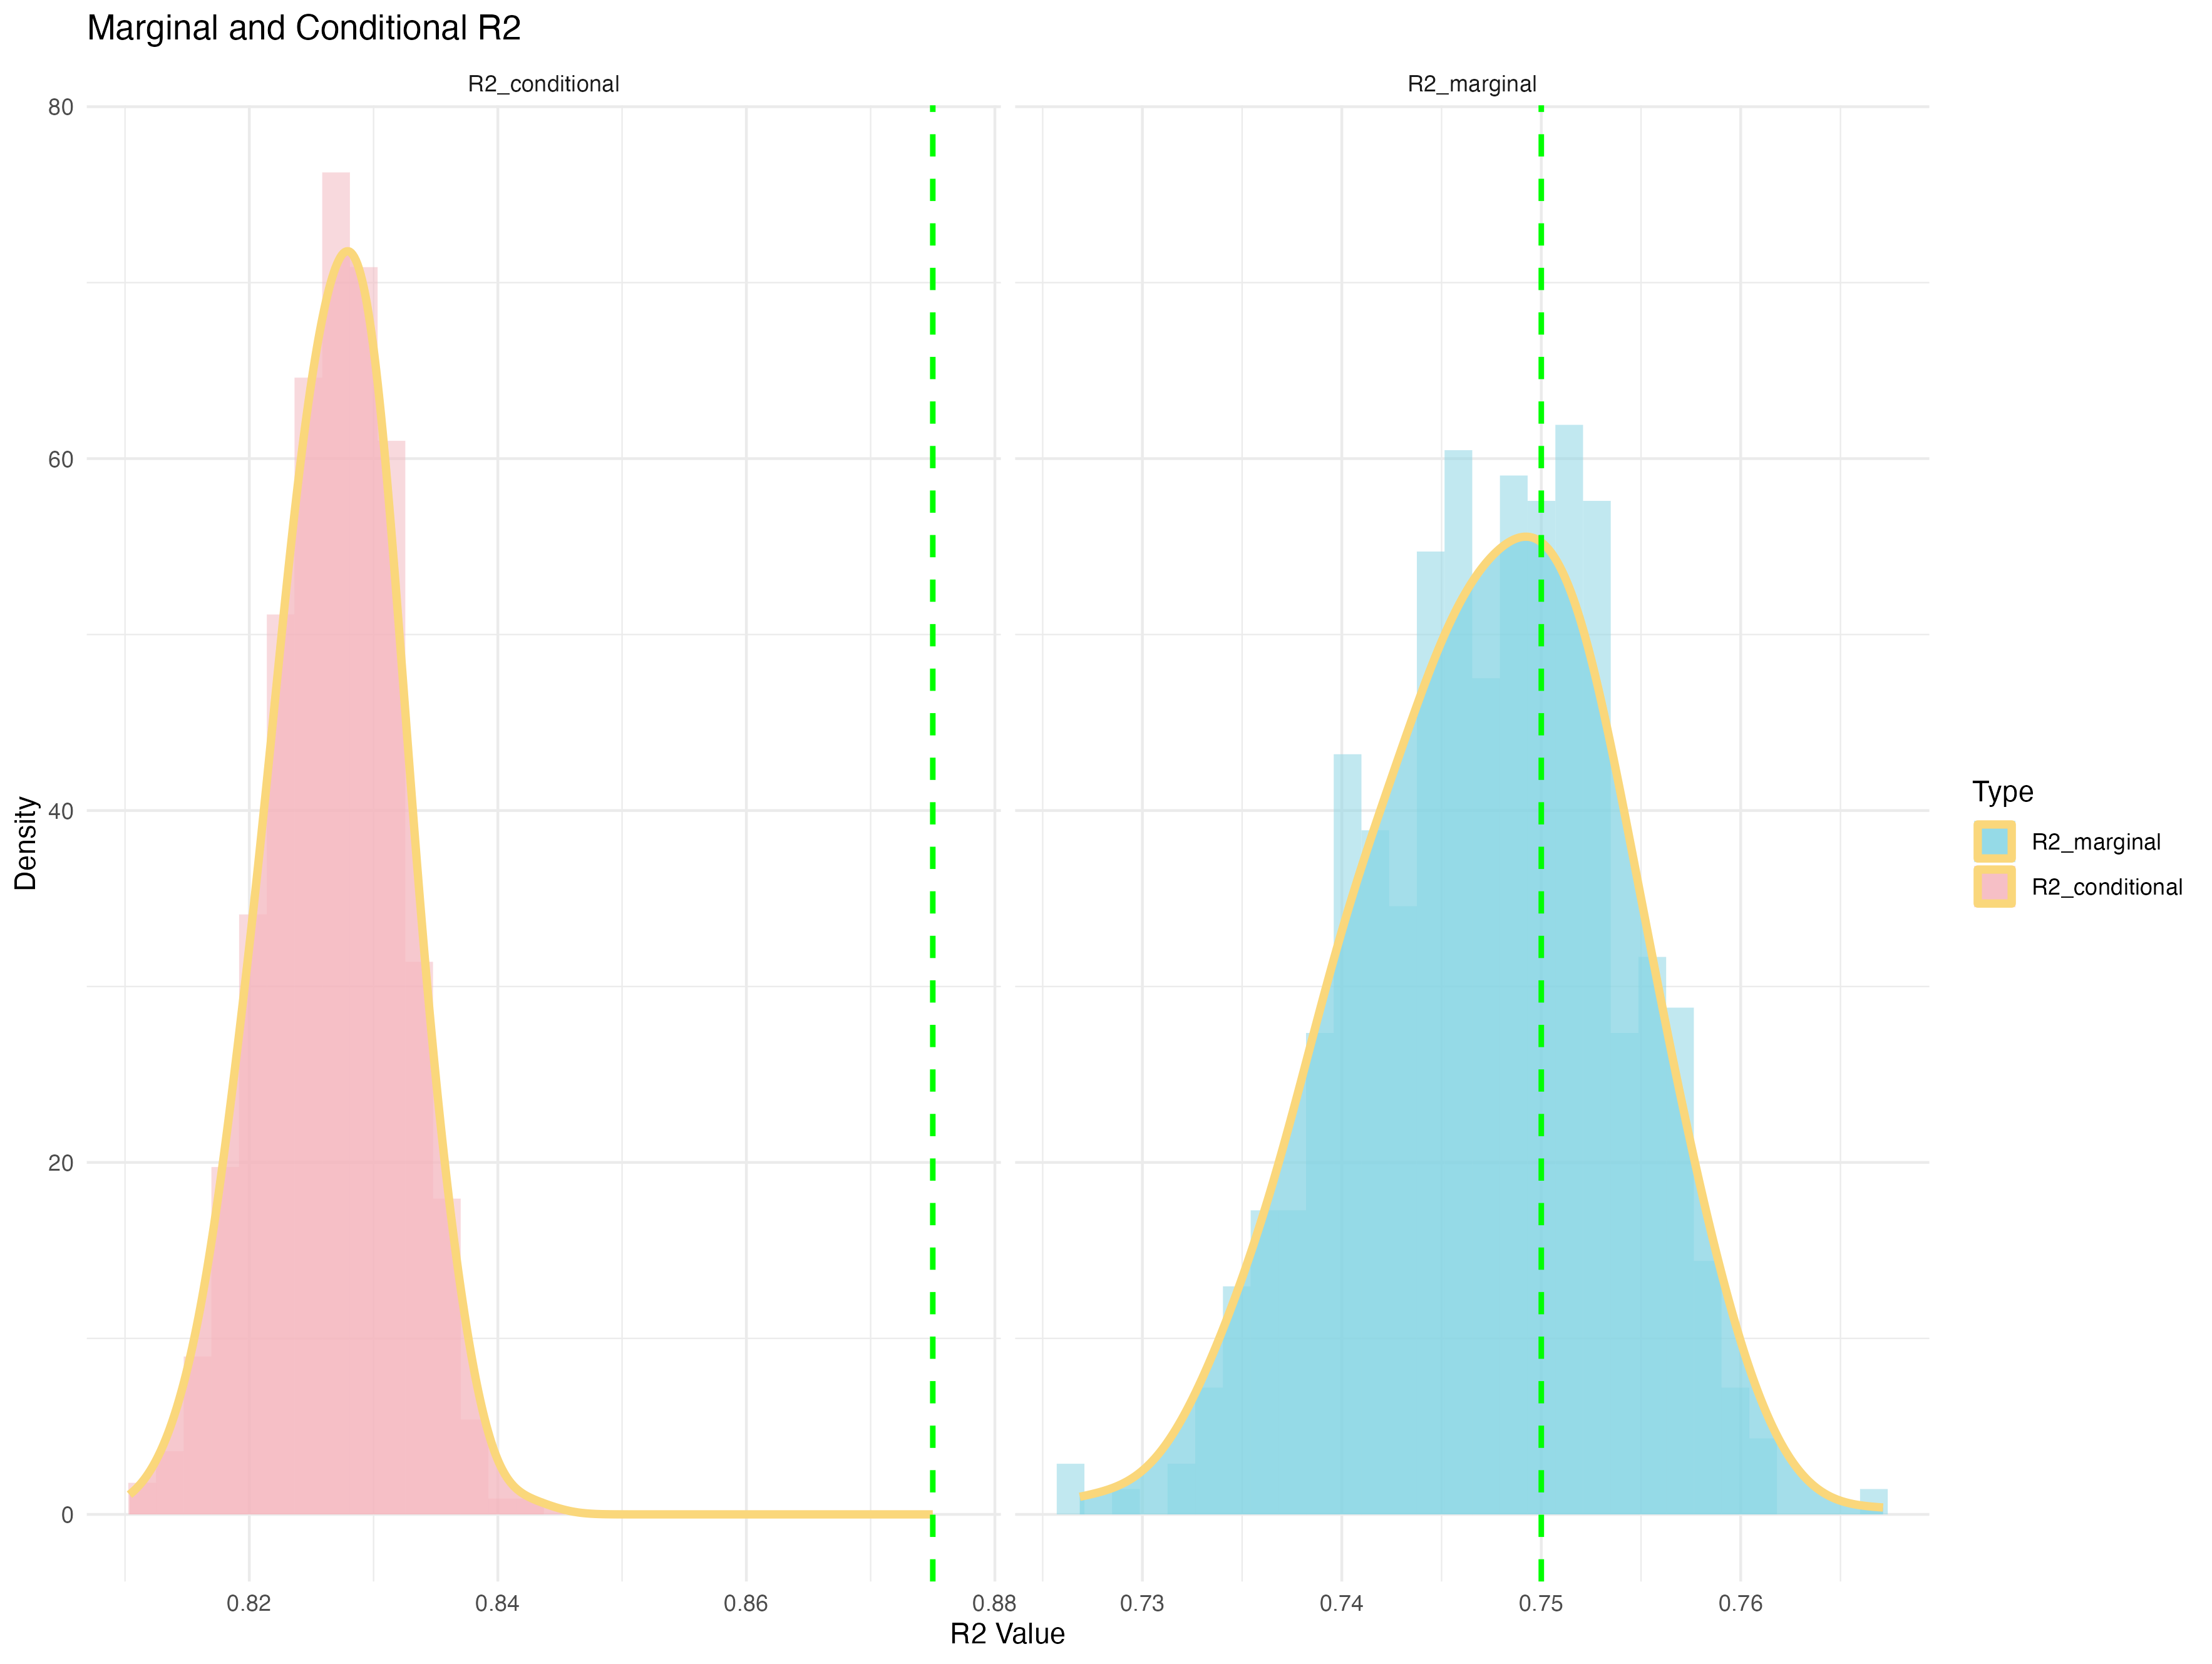
\includegraphics[width=0.7\linewidth]{Figures/Simulation study/Binomial_probit_R2.png}
  %   \caption{Conditional and marginal $R^2$ for binomial GLMM with probit link}
  %     \label{fig:relimp_binomial_probit_r2}
  % \end{figure}
\subsection{Poisson simulation}
The second model fit in the simulation study is a Poisson regression with log-link. The Poisson model was fit with the same correlation levels as the binomial simulation. Further, as was the case for the binomial simulation, we experienced that INLA was not able to fit all $N_{\text{sim}}=500$ simulations. All models were fit for $\rho=0, -0.1$ and $-0.4$, two models crashed for $\rho=0.1$ and we had $84$ unsuccessful model fits for $\rho=0.4$. In \Cref{table:summary_poisson}, a summary of the mean and $95\%$ quantile values for different correlation levels is displayed.
\begin{table}[H]
  \centering
  \begin{tabular}{@{}llcccccc@{}}
    \toprule
    \multicolumn{2}{c}{\textbf{Measure}} & $\mathbf{\rho=0}$ & $\mathbf{\rho=0.1}$ & $\mathbf{\rho=-0.1}$ & $\mathbf{\rho=0.4}$ & $\mathbf{\rho=-0.4}$ \\ \midrule
    \multirow{3}{*}{Random Importance} & Average & 0.1348 & 0.1159 & 0.1560 & 0.0868 & 0.3299 \\
                                       & 2.5\%   & 0.1018 & 0.0914 & 0.1212 & 0.0600 & 0.2713 \\
                                       & 97.5\%  & 0.1689 & 0.1464 & 0.1931 & 0.1072 & 0.3903 \\ \midrule
    \multirow{3}{*}{Fixed Importance X1} & Average & 0.1337 & 0.1552 & 0.1112 & 0.2058 & 0.0385 \\
                                         & 2.5\%   & 0.1251 & 0.1478 & 0.1042 & 0.0002 & 0.0347 \\
                                         & 97.5\%  & 0.1421 & 0.1625 & 0.1195 & 0.2191 & 0.0425 \\ \midrule
    \multirow{3}{*}{Fixed Importance X2} & Average & 0.2672 & 0.2778 & 0.2544 & 0.2853 & 0.1489 \\
                                         & 2.5\%   & 0.2545 & 0.2647 & 0.2407 & 0.0002 & 0.1342 \\
                                         & 97.5\%  & 0.2803 & 0.2881 & 0.2679 & 0.3029 & 0.1648 \\ \midrule
    \multirow{3}{*}{Fixed Importance X3} & Average & 0.4008 & 0.3957 & 0.4039 & 0.3565 & 0.3237 \\
                                         & 2.5\%   & 0.3851 & 0.3799 & 0.3838 & 0.0003 & 0.2939 \\
                                         & 97.5\%  & 0.4185 & 0.4095 & 0.4222 & 0.3784 & 0.3576 \\ \midrule
    \multirow{3}{*}{$R^2_m$}            & Average & 0.8017 & 0.8286 & 0.7695 & 0.8476 & 0.5111 \\
                                         & 2.5\%   & 0.7722 & 0.7981 & 0.7363 & 0.0007 & 0.4639 \\
                                         & 97.5\%  & 0.8304 & 0.8530 & 0.8029 & 0.8960 & 0.5582 \\ \midrule
    \multirow{3}{*}{$R^2_c$}            & Average & 0.9365 & 0.9445 & 0.9255 & 0.9344 & 0.8410 \\
                                         & 2.5\%   & 0.9258 & 0.9354 & 0.9136 & 0.2112 & 0.8149 \\
                                         & 97.5\%  & 0.9467 & 0.9532 & 0.9358 & 0.9660 & 0.8658 \\ \bottomrule
    \end{tabular}
  % \begin{tabular}{@{}llcccccc@{}}
  % \toprule
  % \multicolumn{2}{c}{\textbf{Measure}} & $\mathbf{\rho=0}$ & $\mathbf{\rho=0.1}$ & $\mathbf{\rho=-0.1}$ & $\mathbf{\rho=0.4}$ & $\mathbf{\rho=-0.4}$ \\ \midrule
  % \multirow{3}{*}{Random Importance} & Average & 0.1342 & 0.1156 & 0.1553 & 0.0821 & 0.3304 \\
  %                                    & 2.5\%   & 0.1026 & 0.0908 & 0.1188 & 0.0412 & 0.2643 \\
  %                                    & 97.5\%  & 0.1684 & 0.1438 & 0.1934 & 0.1075 & 0.3957 \\ \midrule
  % \multirow{3}{*}{Fixed Importance X1} & Average & 0.1338 & 0.1553 & 0.1113 & 0.2069 & 0.0384 \\
  %                                      & 2.5\%   & 0.1264 & 0.1473 & 0.1043 & 0.0004 & 0.0339 \\
  %                                      & 97.5\%  & 0.1420 & 0.1629 & 0.1186 & 0.2202 & 0.0424 \\ \midrule
  % \multirow{3}{*}{Fixed Importance X2} & Average & 0.2674 & 0.2780 & 0.2544 & 0.2868 & 0.1489 \\
  %                                      & 2.5\%   & 0.2544 & 0.2667 & 0.2402 & 0.0012 & 0.1320 \\
  %                                      & 97.5\%  & 0.2800 & 0.2892 & 0.2689 & 0.3031 & 0.1653 \\ \midrule
  % \multirow{3}{*}{Fixed Importance X3} & Average & 0.4013 & 0.3959 & 0.4041 & 0.3584 & 0.3230 \\
  %                                      & 2.5\%   & 0.3831 & 0.3810 & 0.3842 & 0.0008 & 0.2897 \\
  %                                      & 97.5\%  & 0.4181 & 0.4091 & 0.4236 & 0.3791 & 0.3561 \\ \midrule
  % \multirow{3}{*}{$R^2_m$}            & Average & 0.8025 & 0.8292 & 0.7698 & 0.8520 & 0.5103 \\
  %                                      & 2.5\%   & 0.7697 & 0.8016 & 0.7366 & 0.0013 & 0.4566 \\
  %                                      & 97.5\%  & 0.8313 & 0.8544 & 0.8045 & 0.8989 & 0.5603 \\ \midrule
  % \multirow{3}{*}{$R^2_c$}            & Average & 0.9367 & 0.9448 & 0.9251 & 0.9341 & 0.8407 \\
  %                                      & 2.5\%   & 0.9262 & 0.9353 & 0.9126 & 0.1786 & 0.8132 \\
  %                                      & 97.5\%  & 0.9467 & 0.9530 & 0.9356 & 0.9662 & 0.8667 \\ \bottomrule
  % \end{tabular}
  \caption{Summary of simulation study results for the quantiles of relative importance estimates the Poisson model across different correlation levels.}
  \label{table:summary_poisson}
\end{table}
\subsubsection{Fixed effects}
As for the binomial, we first look at the fixed effects. The estimates of posterior relative importance for the fixed effects (\Cref{fig:fixed_combined_poisson}) are very similar in shape as the binomial model. The first thing to note is that for the case $\rho=0.4$, we see that the distribution of relative importance of all covariates contains values very close to zero. After some investigation of the fitted models, it turns out that INLA sometimes returns a model that estimates all fixed coefficients to be $0$, but estimates the random effect almost as expected. One might expect that such a model is not sensible and that it should have crashed, but it seems that the model does not crash and has therefore been included in results of the simulation study. With the coefficients estimated to be close to zero, the model will consequently estimate the relative importance of the fixed effects close to zero. It is therefore plausible to believe that the method correctly estimates relative importance, and that this model fit might be caused by some problem with the simulated dataset or INLA.
\\
\\
Disregarding the close to zero values for $\rho=0.4$, the overall estimates are larger for the Poisson model, which is mainly due to the log-link function having a smaller associated distributional variance than the logit-link and therefore the contribution by the fixed effects becomes larger. It seems the estimates form a normal curve about the mean, and for $\rho=0$ the average estimated importance is close to the expected value. The same influence of varying correlation levels can be seen as in the binomial model, namely that we obtain larger importance of the fixed effects when the correlation increases. Again the difference is notably large, with the average relative importance of $X_1$ going from $0.0385$ for $\rho=-0.4$ to $0.2058$ for $\rho=0.4$. For $X_2$ and $X_3$ the average relative importance increases from $0.1489$ to $0.2853$ and from $0.3237$ to $0.3565$ respectively.
\\
\\
Further, we see the same pattern of larger increase in importance to $X_1$ than for $X_2$ and larger for $X_2$ than $X_3$, as for the binomial model, when correlation increases from $\rho=0$ to $\rho=0.4$. For the Poisson model, it can be seen that for $\rho=0$, $X_3$ is on average allocated an importance of $0.4008$, and when $\rho=0.4$, we have no importance estimates larger than $0.4$. This is in line with what one would expect, when the off diagonal elements of $\boldsymbol{\Lambda}$ become large enough so that the distributed importance to the covariate with the largest coefficient becomes smaller with increasing correlation. Contrary, $X_1$ is again allocated the largest increase and $X_2$ is allocated a larger increase in importance than $X_3$ but smaller than $X_1$. For the case $\rho=0$, we see that the mean of our samples and the expected relative importance (\Cref{table:2}) are very close, and it seems the model express the expected pattern of relative importance for varying correlation levels.
% \begin{figure}[H]
%   \centering
%   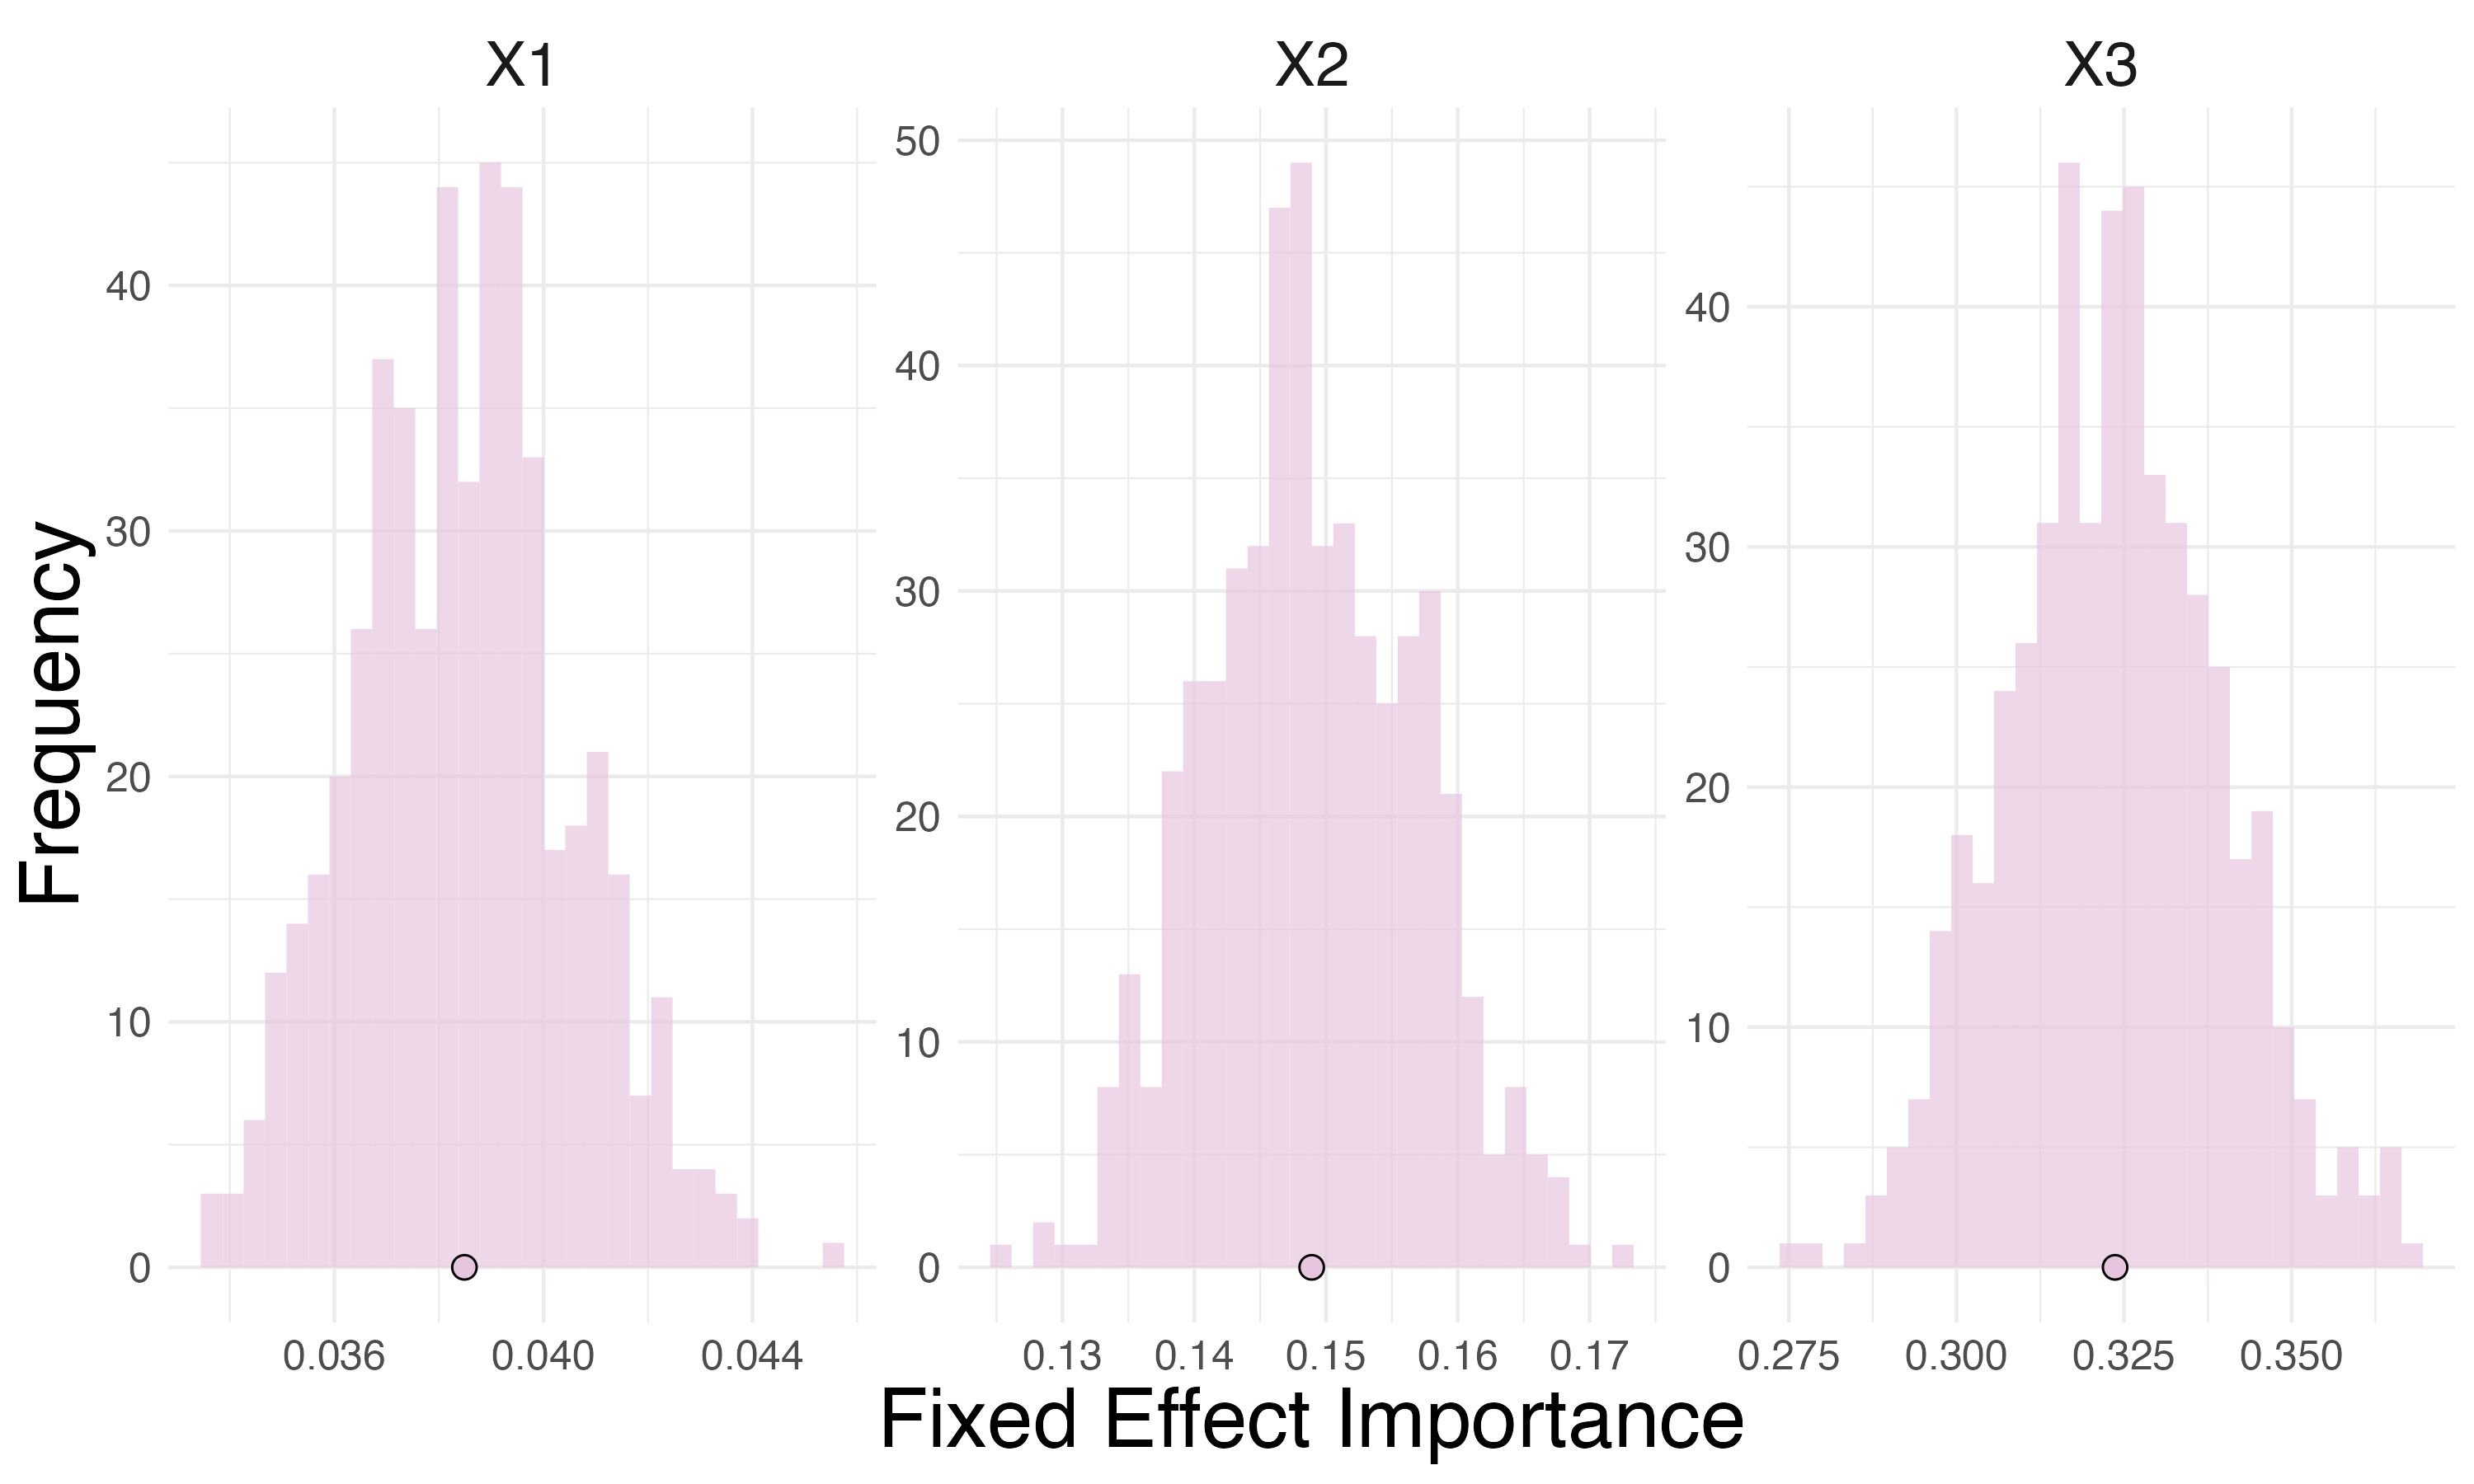
\includegraphics[width=1\linewidth]{Figures/Simulation study/Fixed_high_neg_poisson.png}
%   \caption{Histogram with relative importance estimates for the fixed effects in the Poisson regression with different correlation levels $\rho$. The values are estimated from $N_{\text{sim}}=500$ simulations by the Bayesian Variable Importance method in the simulation study. The regression coefficients are set to be  $\boldsymbol{\beta}=(1, \sqrt{2}, \sqrt{3})^T$ and the vertical green line in (c) is the expected relative importance in the case of uncorrelated data. The mean of the relative importance for all simulations is denoted at the bottom of each histogram as a circle. (a) Relative importance of the fixed effects $\mathbf{X_1},  \mathbf{X}_2, \mathbf{X}_3$ for $\rho=-0.4$.}
%   \label{fig:fixed_effects_poisson_high_neg}
% \end{figure}
% \begin{figure}[H]\ContinuedFloat
%   \centering
%   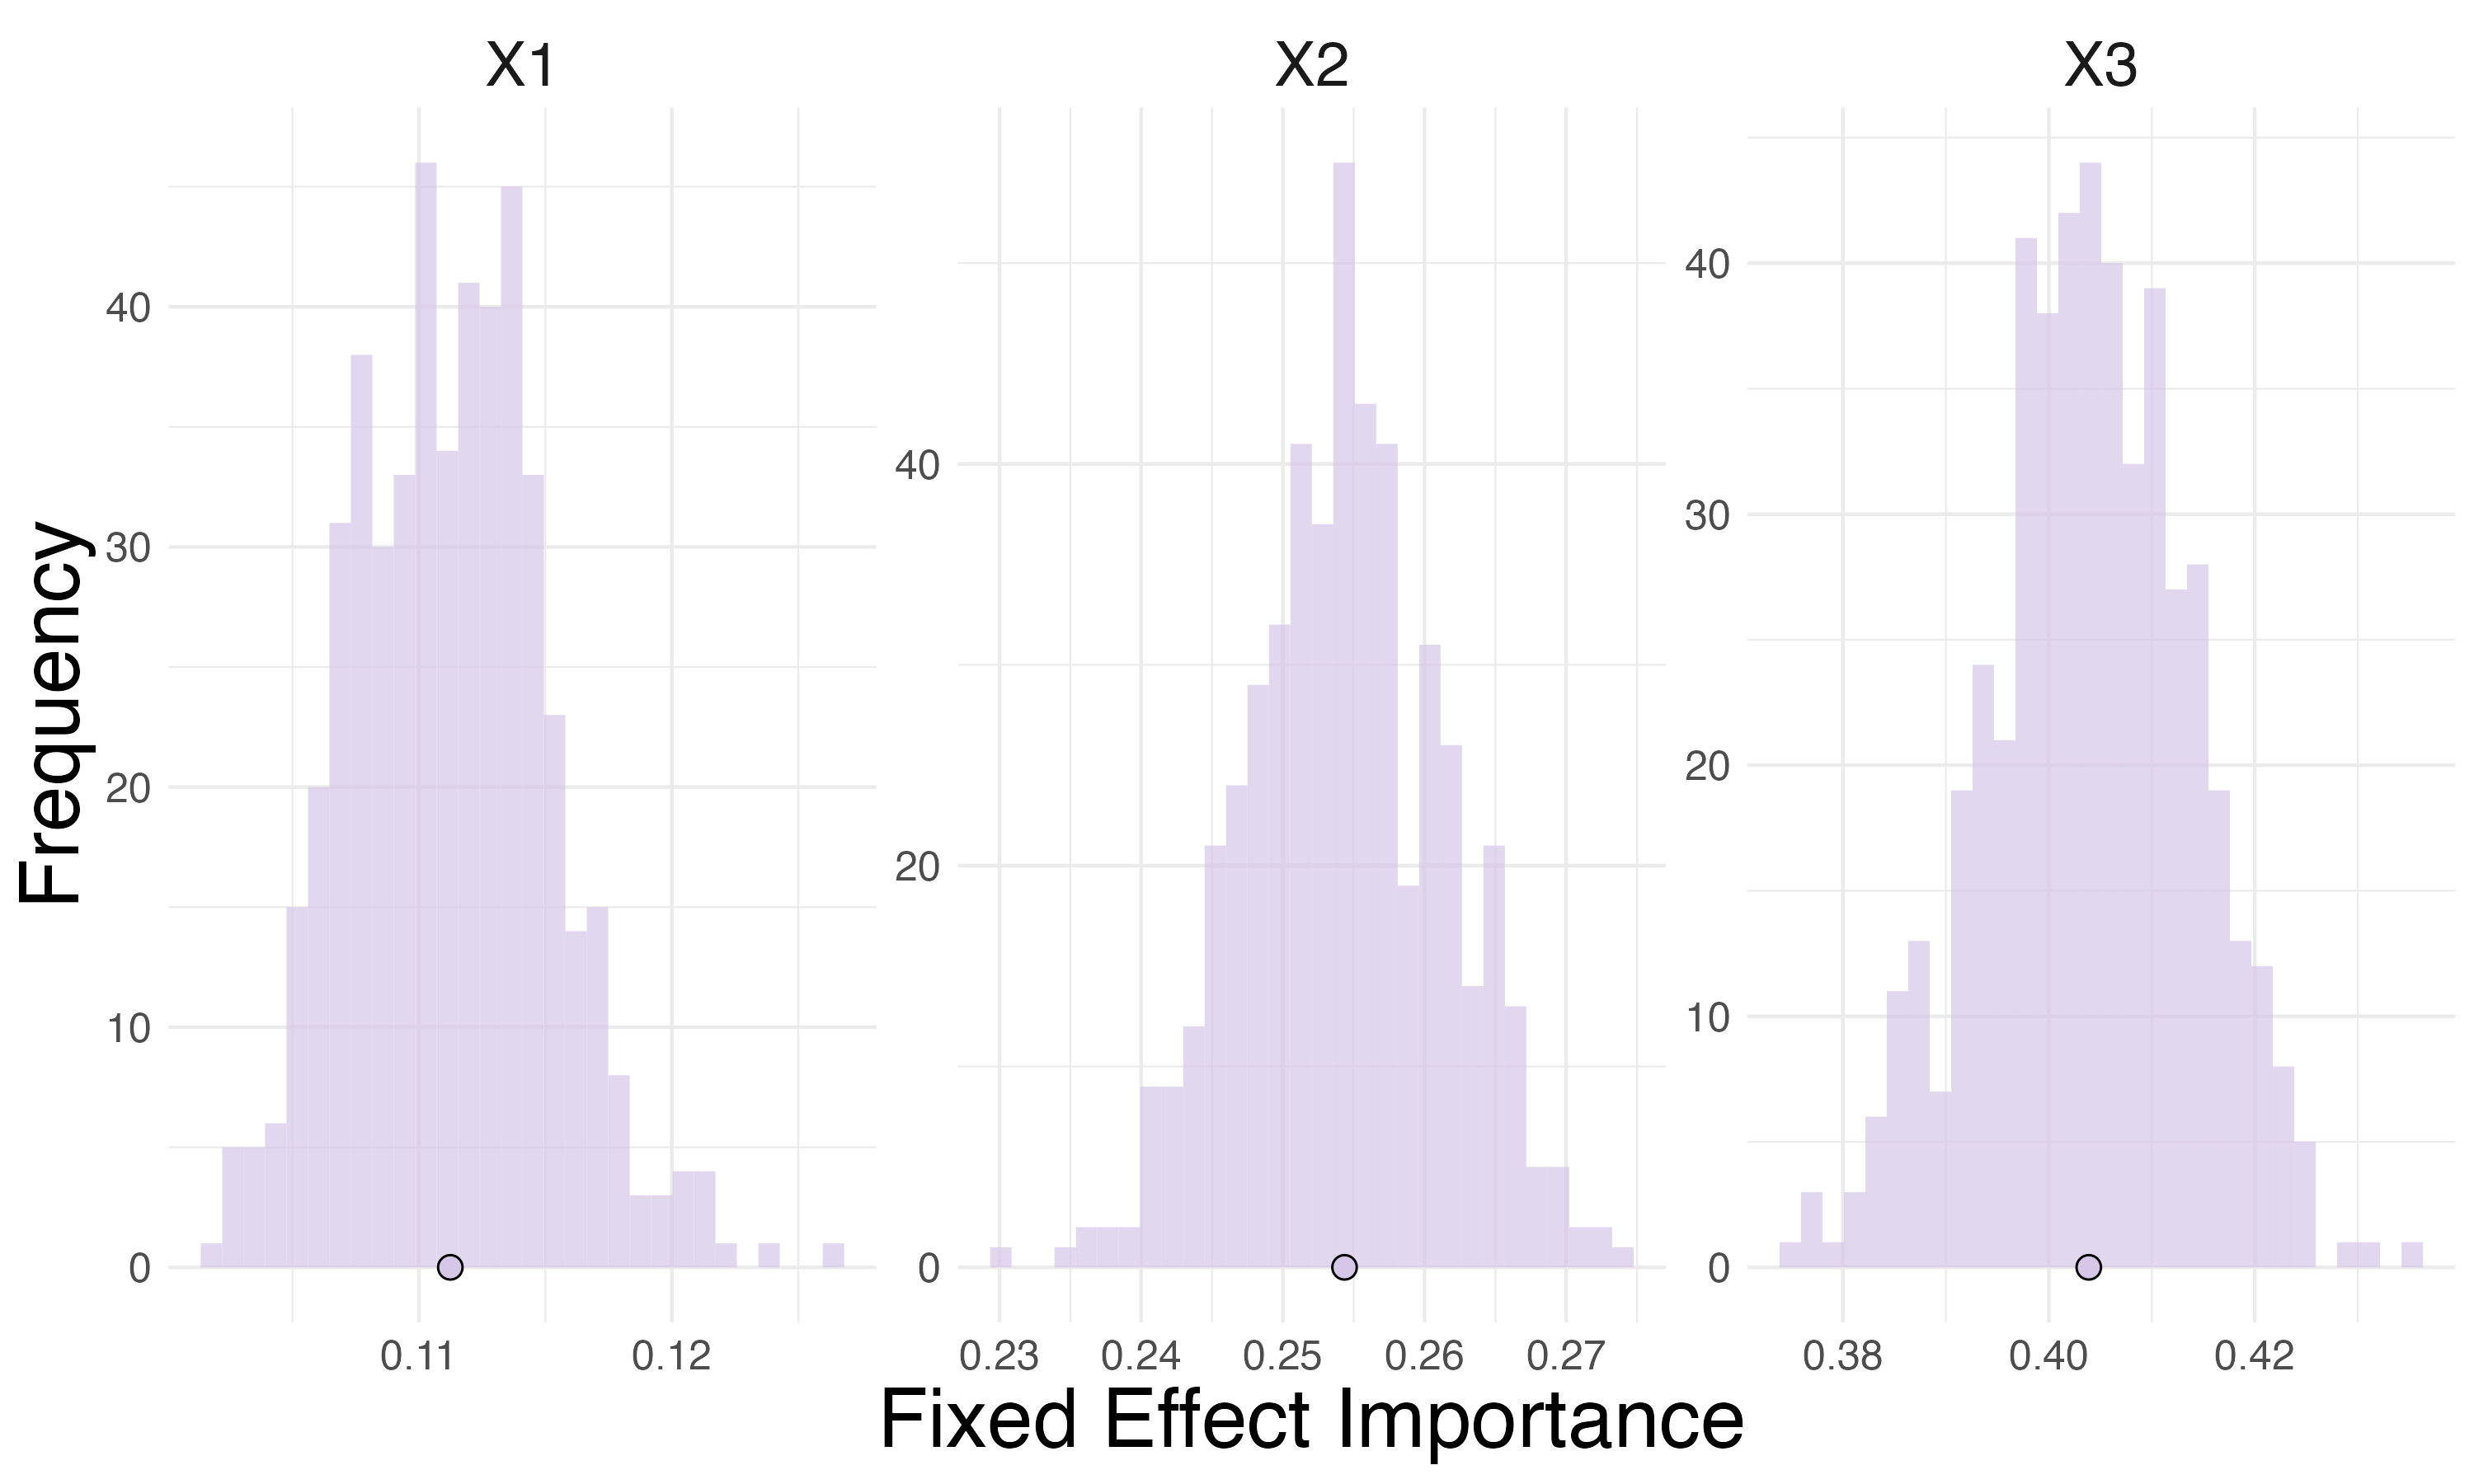
\includegraphics[width=1\linewidth]{Figures/Simulation study/Fixed_low_neg_poisson.png}
%   \caption{(b) Relative importance of the fixed effects $\mathbf{X_1},  \mathbf{X}_2, \mathbf{X}_3$ for $\rho=-0.1$.}
%   \label{fig:fixed_effects_poisson_low_neg}
% \end{figure}
% \begin{figure}[H]\ContinuedFloat
%   \centering
%   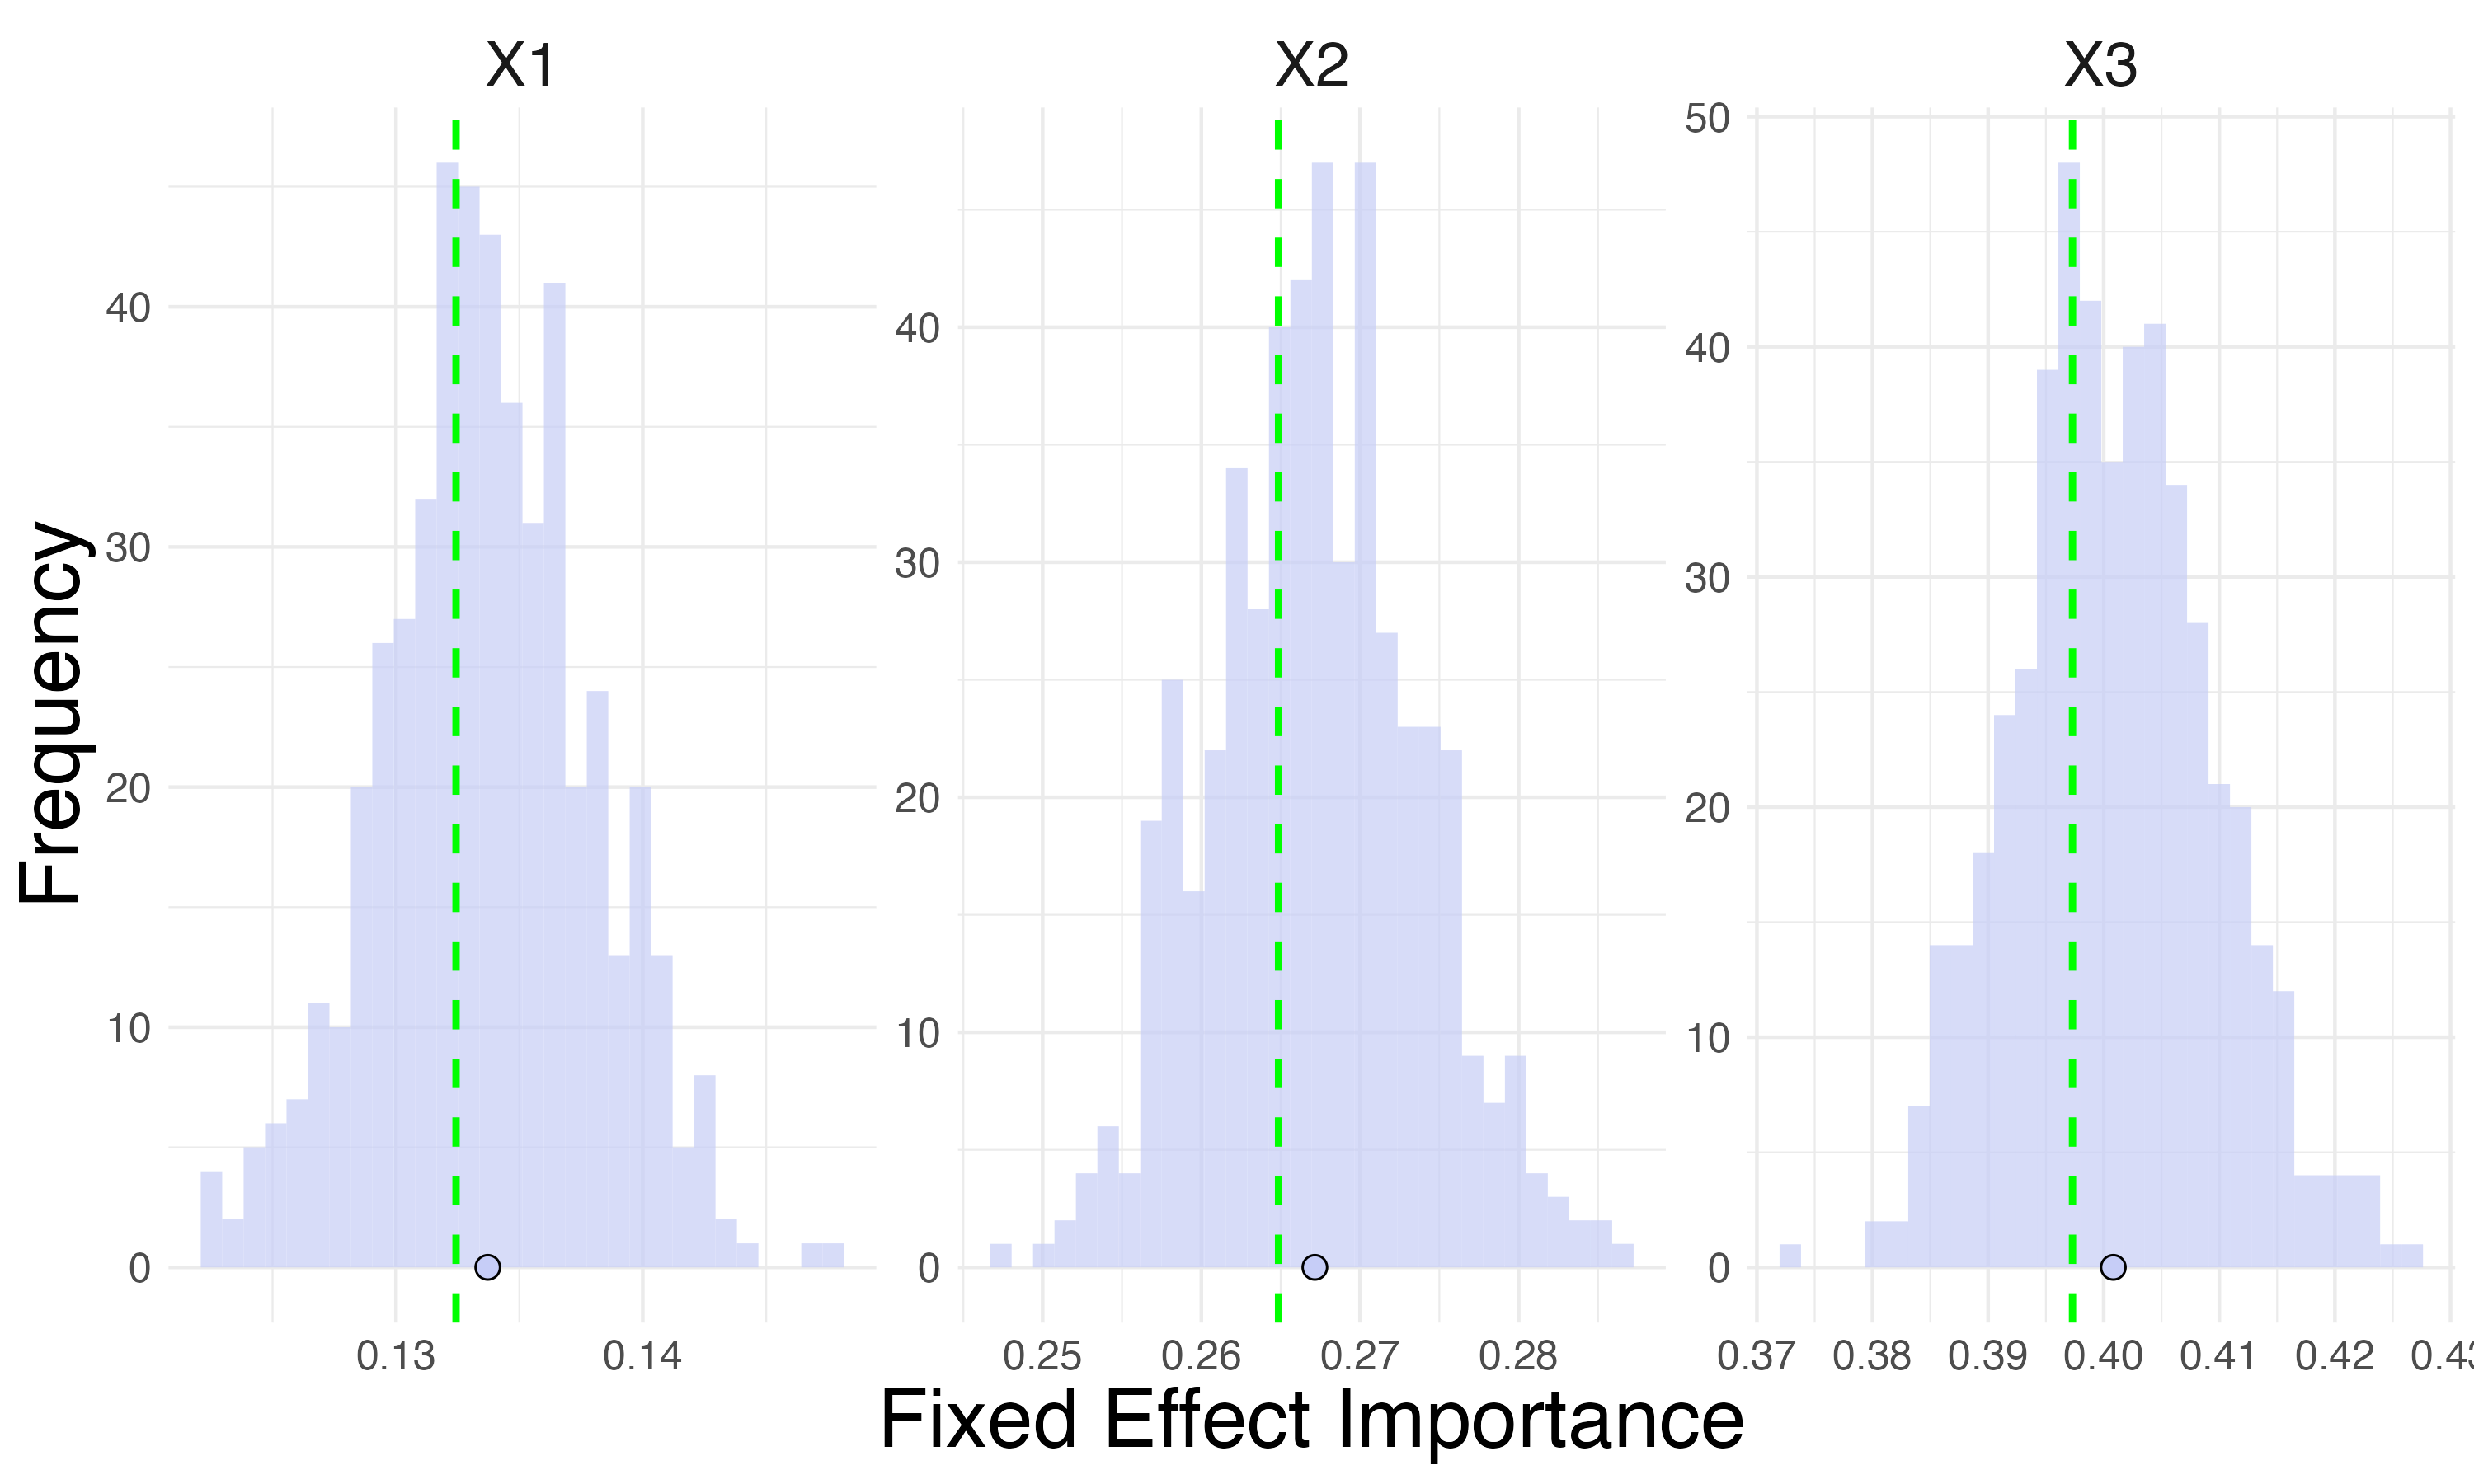
\includegraphics[width=1\linewidth]{Figures/Simulation study/Fixed_no_poisson.png}
%   \caption{(c) Relative importance of the fixed effects $\mathbf{X_1},  \mathbf{X}_2, \mathbf{X}_3$ for $\rho=0$.}
%   \label{fig:fixed_effects_poisson_no}
% \end{figure}
% \begin{figure}[H]\ContinuedFloat
%   \centering
%   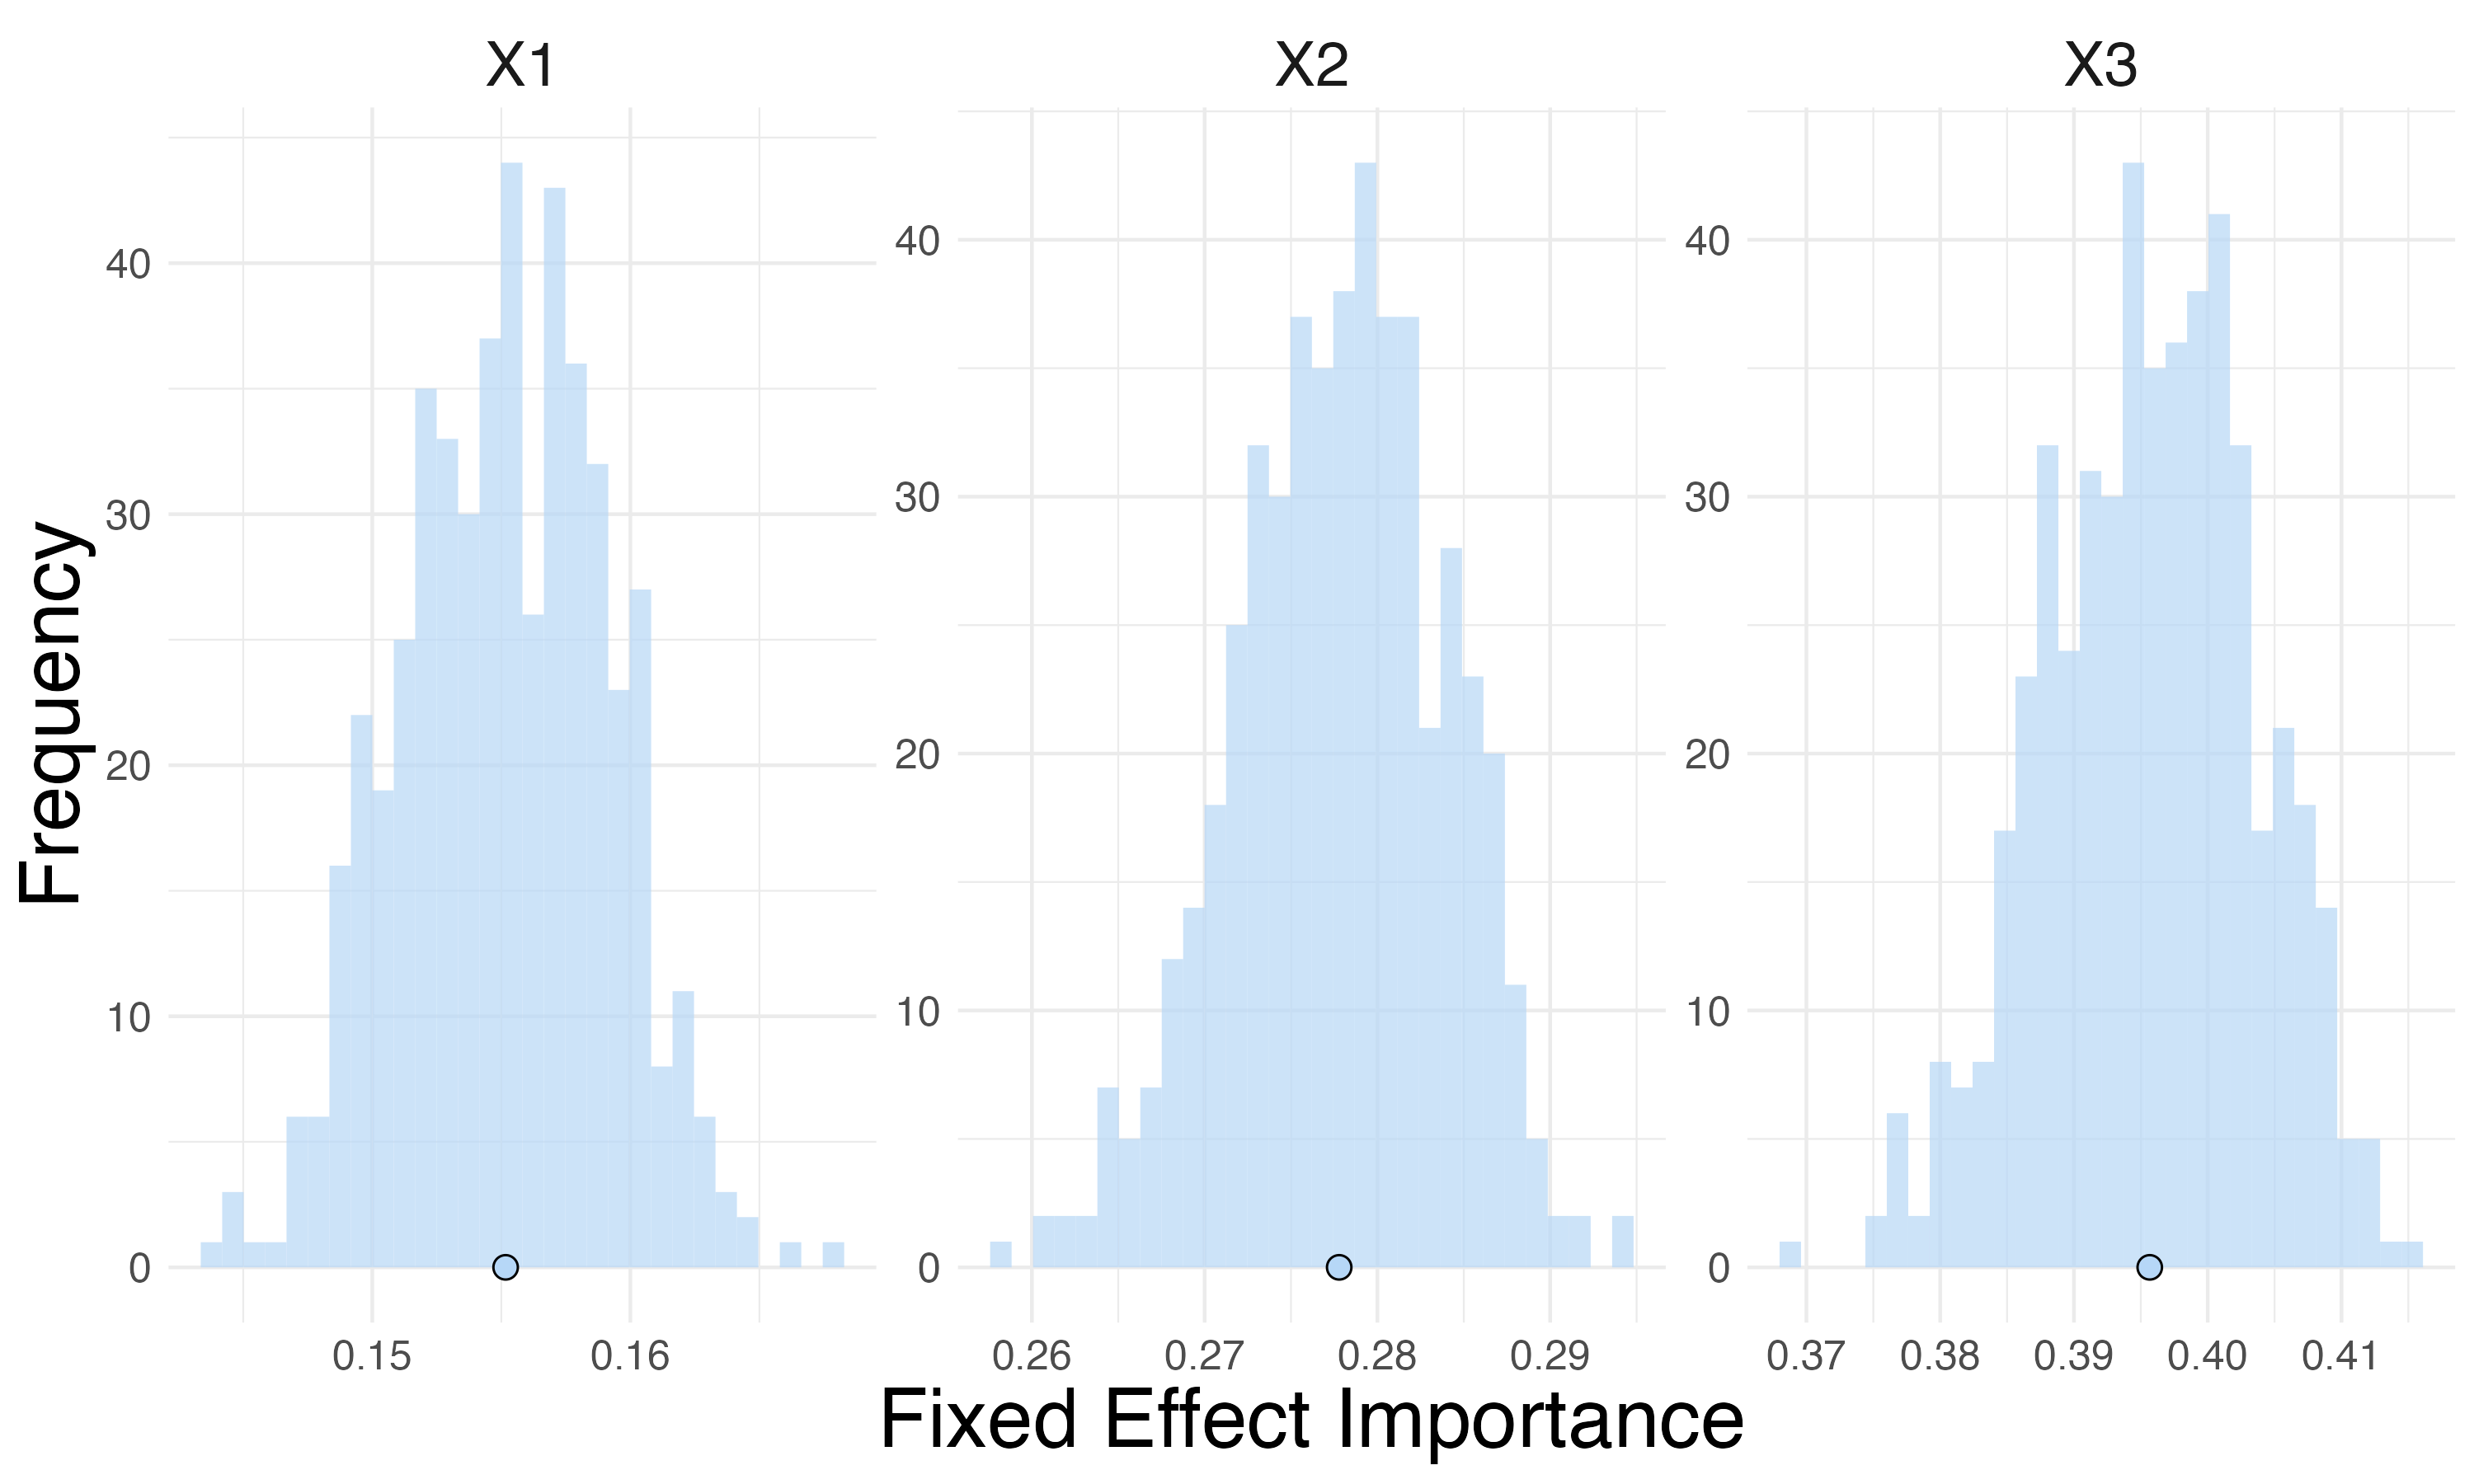
\includegraphics[width=1\linewidth]{Figures/Simulation study/Fixed_low_pos_poisson.png}
%   \caption{(d) Relative importance of the fixed effects $\mathbf{X_1},  \mathbf{X}_2, \mathbf{X}_3$ for $\rho=0.1$.}
%   \label{fig:fixed_effects_poisson_low_pos}
% \end{figure}
% \begin{figure}[H]\ContinuedFloat
%   \centering
%   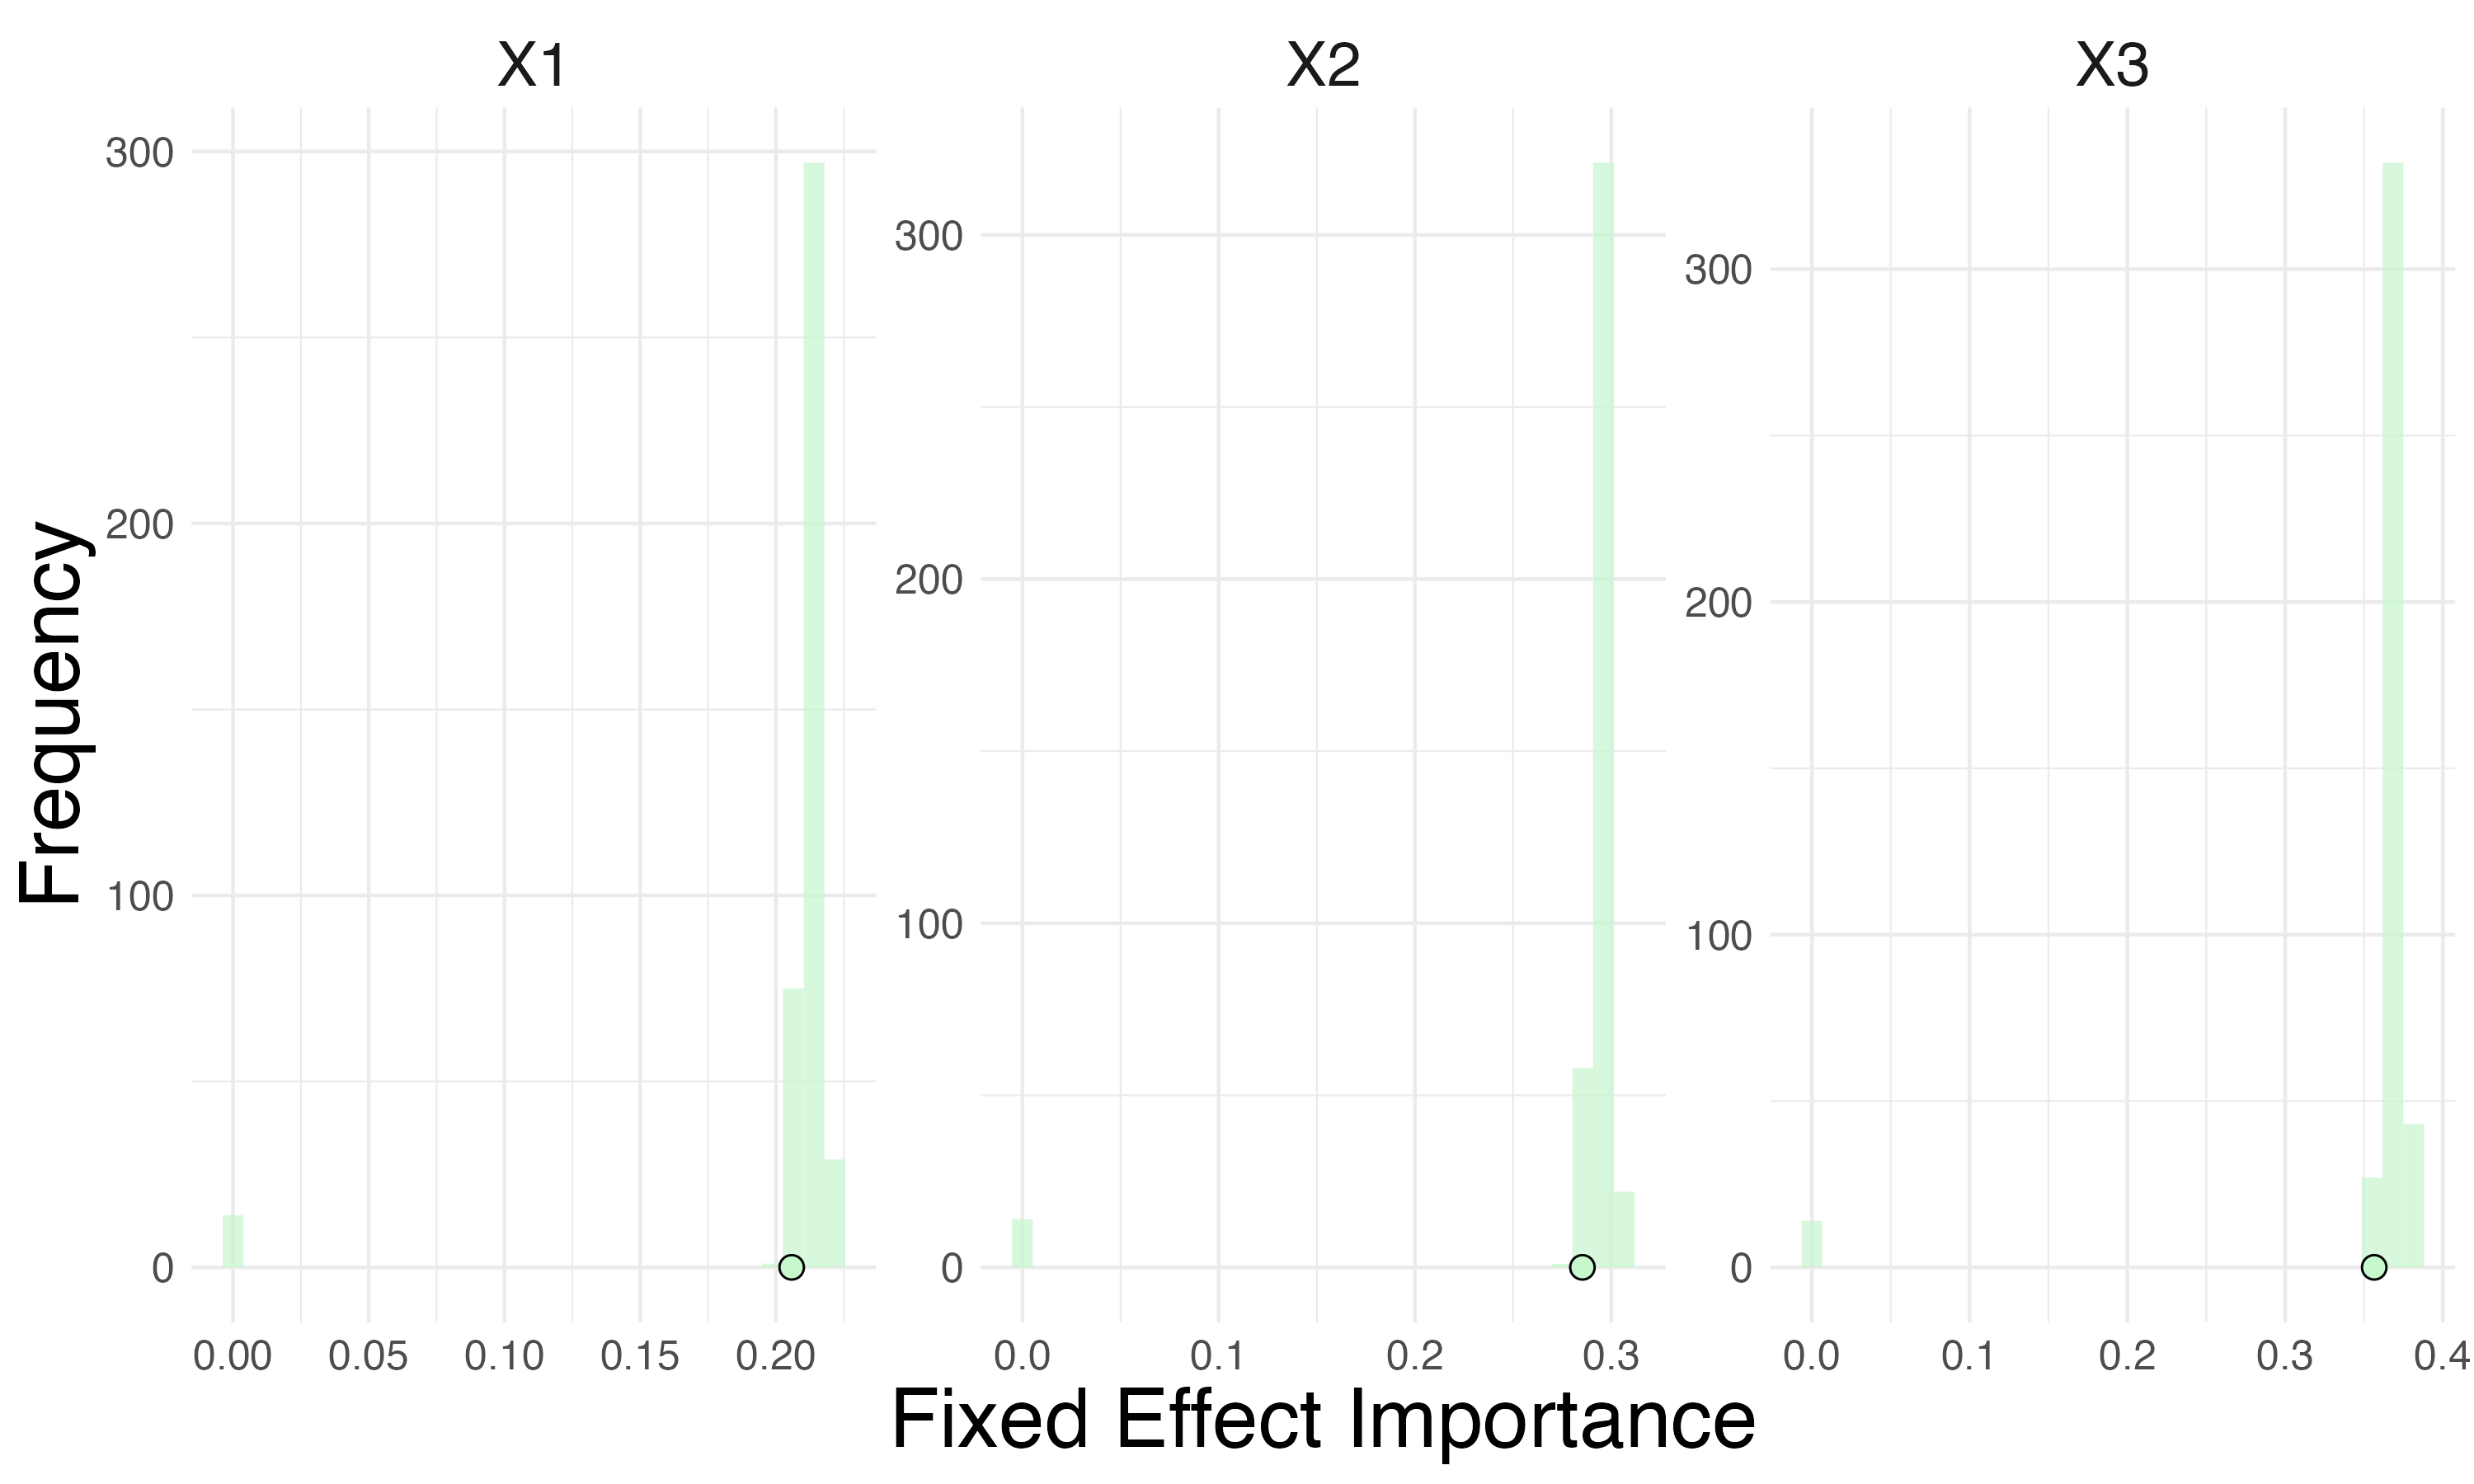
\includegraphics[width=1\linewidth]{Figures/Simulation study/Fixed_high_pos_poisson.png}
%   \caption{(e) Relative importance of the fixed effects $\mathbf{X_1},  \mathbf{X}_2, \mathbf{X}_3$ for $\rho=0.4$.}
%   \label{fig:fixed_effects_poisson_high_pos}
% \end{figure}

% \begin{figure}[H]
%   \centering
%   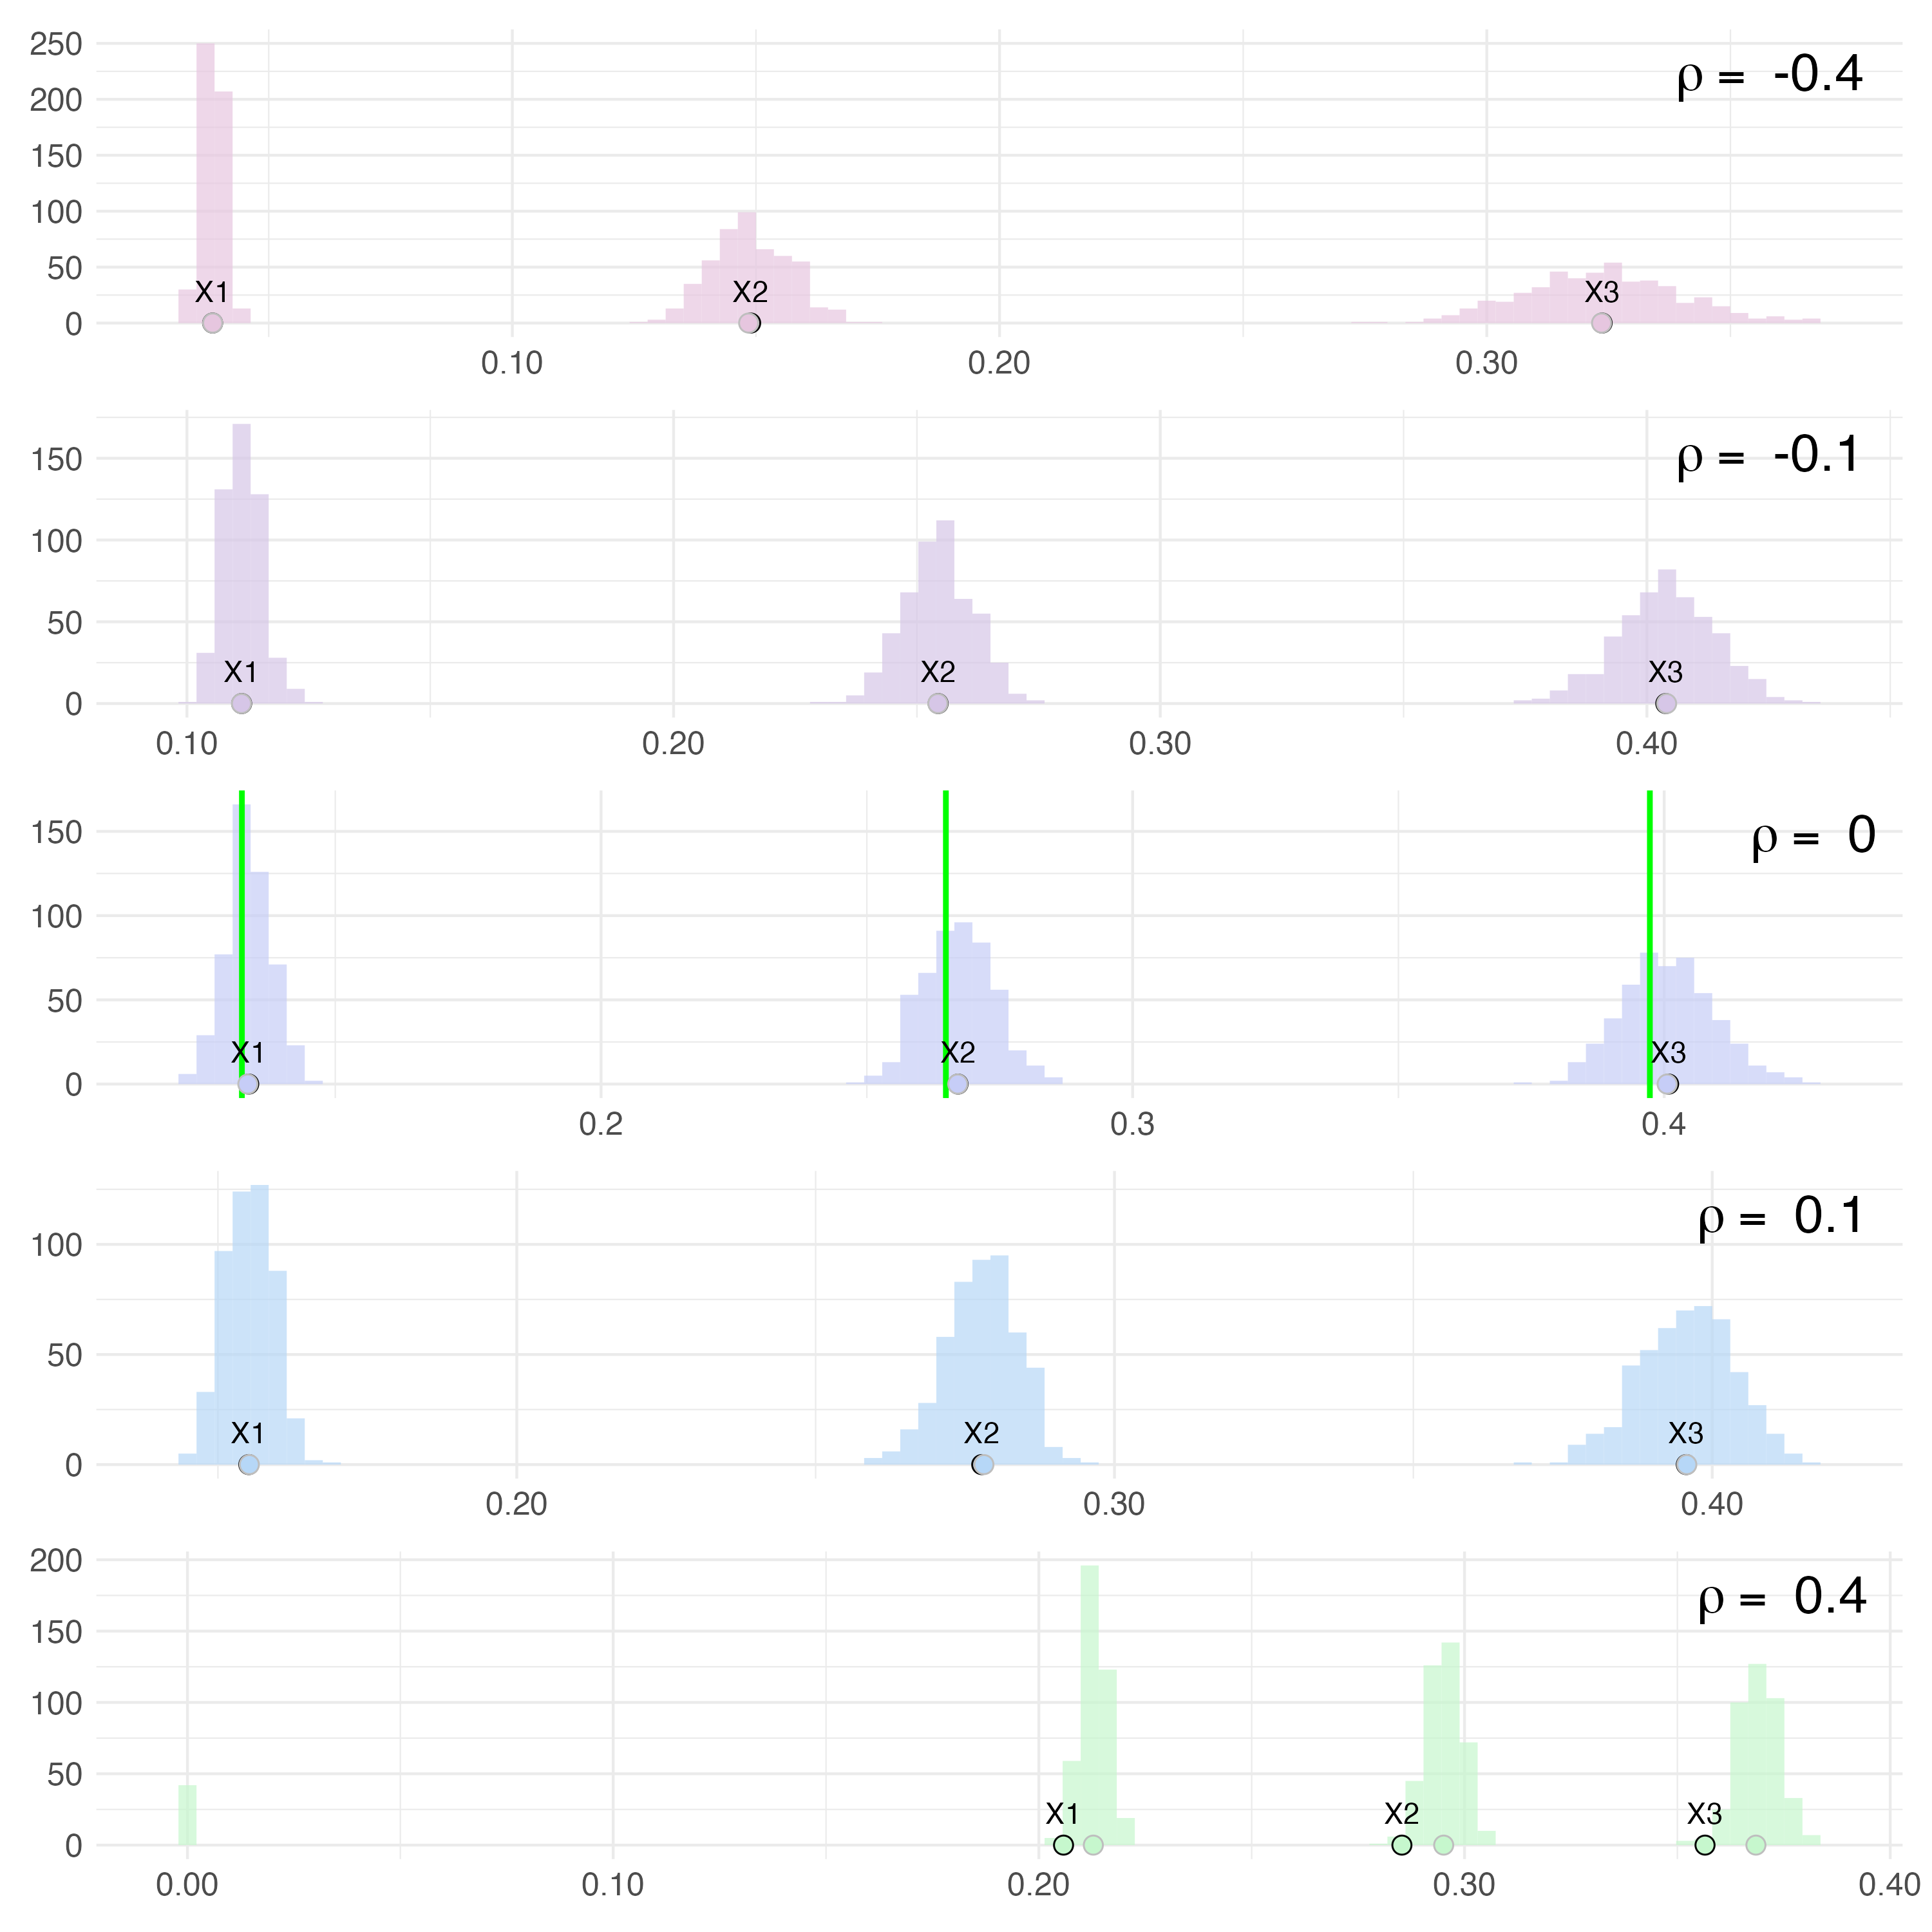
\includegraphics[width=1\linewidth]{Figures/Simulation study/Fixed_combined_poisson.png}
%   \caption{(e) Relative importance of the fixed effects $\mathbf{X_1},  \mathbf{X}_2, \mathbf{X}_3$ for $\rho=0.4$.}
%   \label{fig:fixed_combined_poisson}
% \end{figure}

\begin{figure}[H]
  \centering
  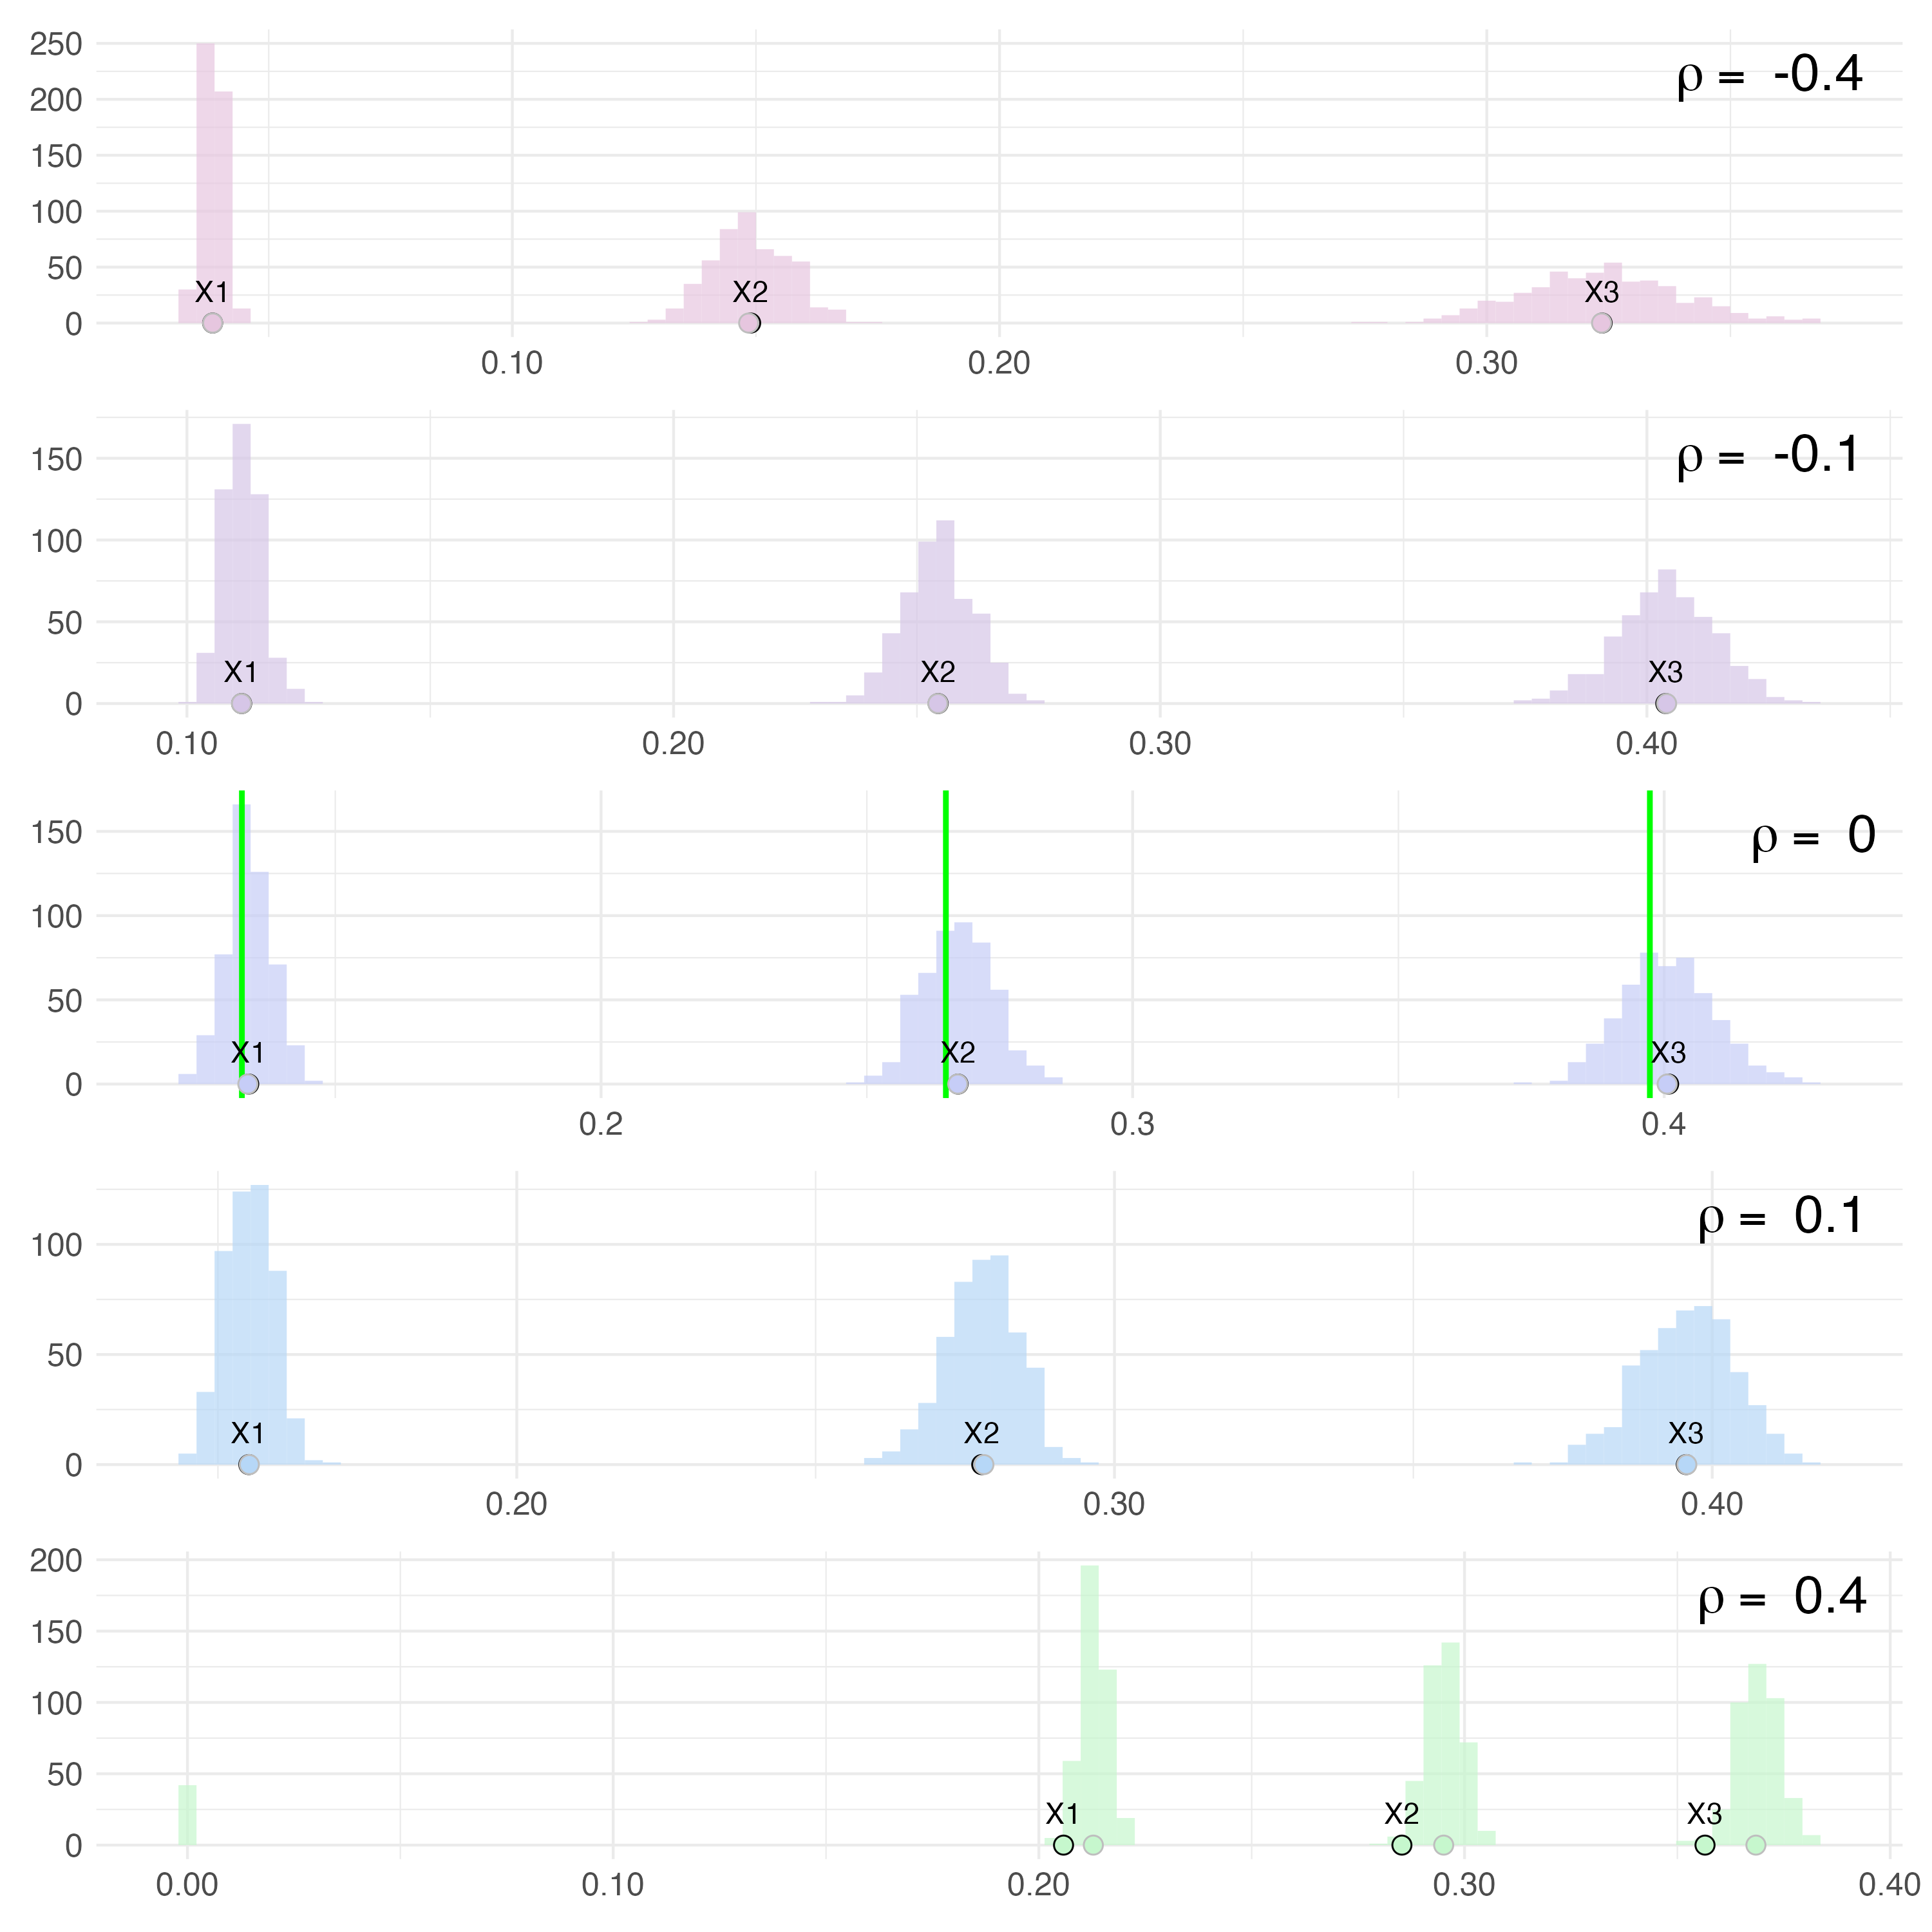
\includegraphics[width=1.1\linewidth]{Figures/Simulation study/Fixed_combined_poisson.png}
  \caption{Histogram with relative importance of the fixed effects present in the poisson regression for the different correlation levels $\rho=-0.4$ (top), $\rho=-0.1$ (second from the top), $\rho=0$ (middle), $\rho=0.1$ (second from bottom) and $\rho=0.4$ (bottom). The values are calculated by the Bayesian Variable Importance method from the $N_{\text{sim}}=500$ simulations in the simulation study. The true regression coefficients are $\boldsymbol{\beta}=(1, \sqrt{2}, \sqrt{3})^T$ and the vertical green line for $\rho=0$ displays the expected relative importance in the case of uncorrelated data. The mean of the relative importance for all simulations is denoted at the bottom of each histogram as a circle.}
  \label{fig:fixed_combined_poisson}
\end{figure}
\subsubsection{Random effect}
When looking at the sampled posterior distribution of relative importance estimates of the random effect in the Poisson mode (\Cref{fig:relimp_random_poisson}), we see that they too are in general a bit larger than the same estimates for the binomial case. This is again a consequence of the smaller distributional variance, and so we expect these results. The shrinkage effect of increasing correlation is also here apparent, with the average relative importance of the random effect going from $0.3299$ for $\rho=-0.4$ to $0.0868$ for $\rho=0.4$. The expected value when $\rho=0$ is $0.1338$ as shown in \Cref{table:2}, and we see that the average estimate is close to this value. The orange dots, denoting the estimates form the \texttt{rptR} package are close to the average estimate from the BVI method, with the largest difference being seen for $\rho=-0.1$ with a difference of $0.0260$.
\\
\\
As previously mentioned, for $\rho=0.4$, some models estimated all the fixed effects to be zero. As a consequence of this, the random effect for these models are in turn estimated to have a corresponding larger importance,  due to the way we have defined relative importance. Although it is not so clear from \Cref{fig:relimp_random_poisson}, it can be seen that we have values of approximately $0.3$, $0.9$ and $1$ when $\rho=0.4$. Again, albeit unfortunate, we believe that the method correctly estimates the relative importance, based on the given model, and that the fitted models might be results of some problem with the simulated data or INLA.
\begin{figure}[H]
  \centering
    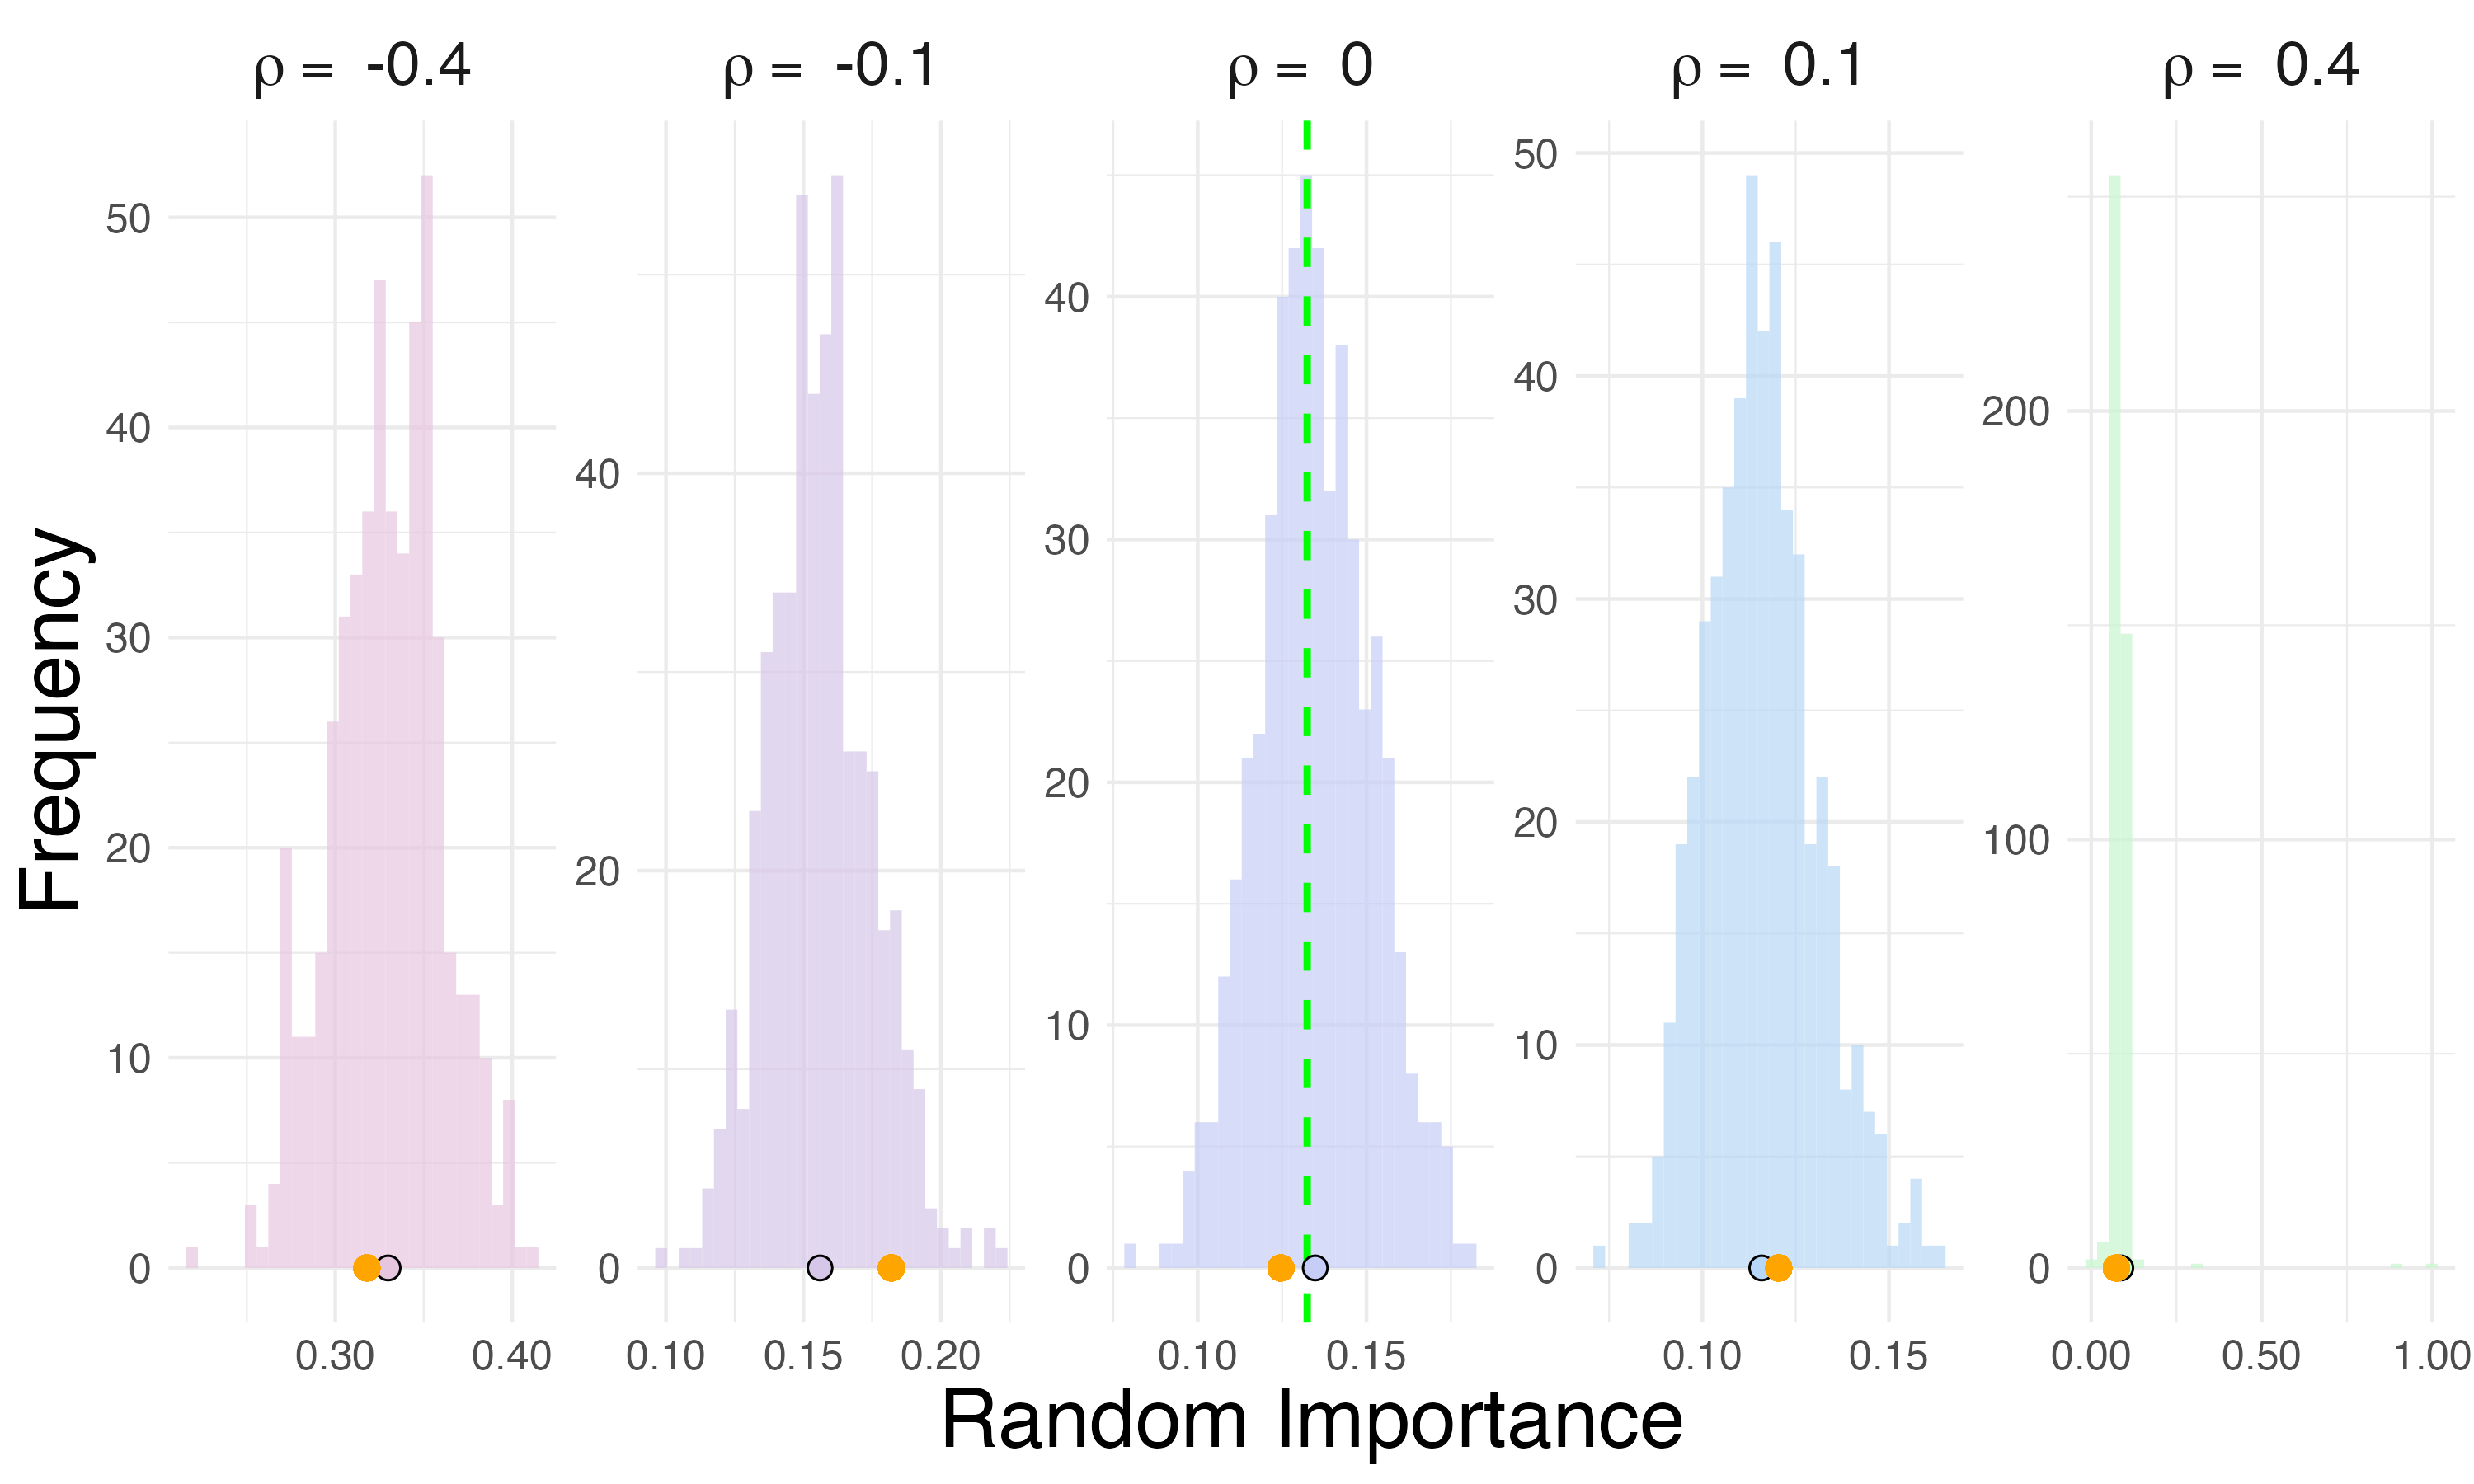
\includegraphics[width=1\linewidth]{Figures/Simulation study/Random_poisson.png}
    \caption{Histogram with relative importance estimates for the random effect $\boldsymbol{\alpha}$ for varying values of $\rho$ calculated by the BVI method. The study conducted $N_{\text{sim}}=500$ simulations and the mean of the relative importance for all simulations is displayed at the bottom of each histogram as a circle. The vertical green line for $\rho=0$ is the expected relative importance as in \Cref{table:2}.}
    \label{fig:relimp_random_poisson}
\end{figure}
\subsubsection{$R^2$ estimates}
Moving on to the estimated posterior $R^2$ distributions for the Poisson model (\Cref{fig:r2_combined_poisson}), we see that the expected values from \Cref{table:r2values} are in close agreement with the average marginal and conditional $R^2$ estimated from the BVI method for all correlation levels. The largest difference in expected values and average values from the BVI method is found for $\rho=0.4$ and is $0.0286$ and $0.0263$ for the marginal and conditional $R^2$ respectively. As can be seen in \Cref{fig:r2_combined_poisson}, we have some values close to zero. This is likely another consequence of the fixed effects sometimes being estimated to be zero, causing our method to estimate the marginal $R^2$ values close to zero. The conditional $R^2$ values have some instances where it is much lower than expected, which is likely a consequence of a strange estimate for the importance of $\boldsymbol{\alpha}$ being propagated to the conditional $R^2$. The estimates from the \texttt{rptR} package deviate quite a bit from our method, and are consistently larger for both marginal and conditional $R^2$. Overall, the distributions seem to form a reasonably symmetric normal curve centered at the mean, close to what we would expect.
% \begin{figure}[H]
%   \centering
%   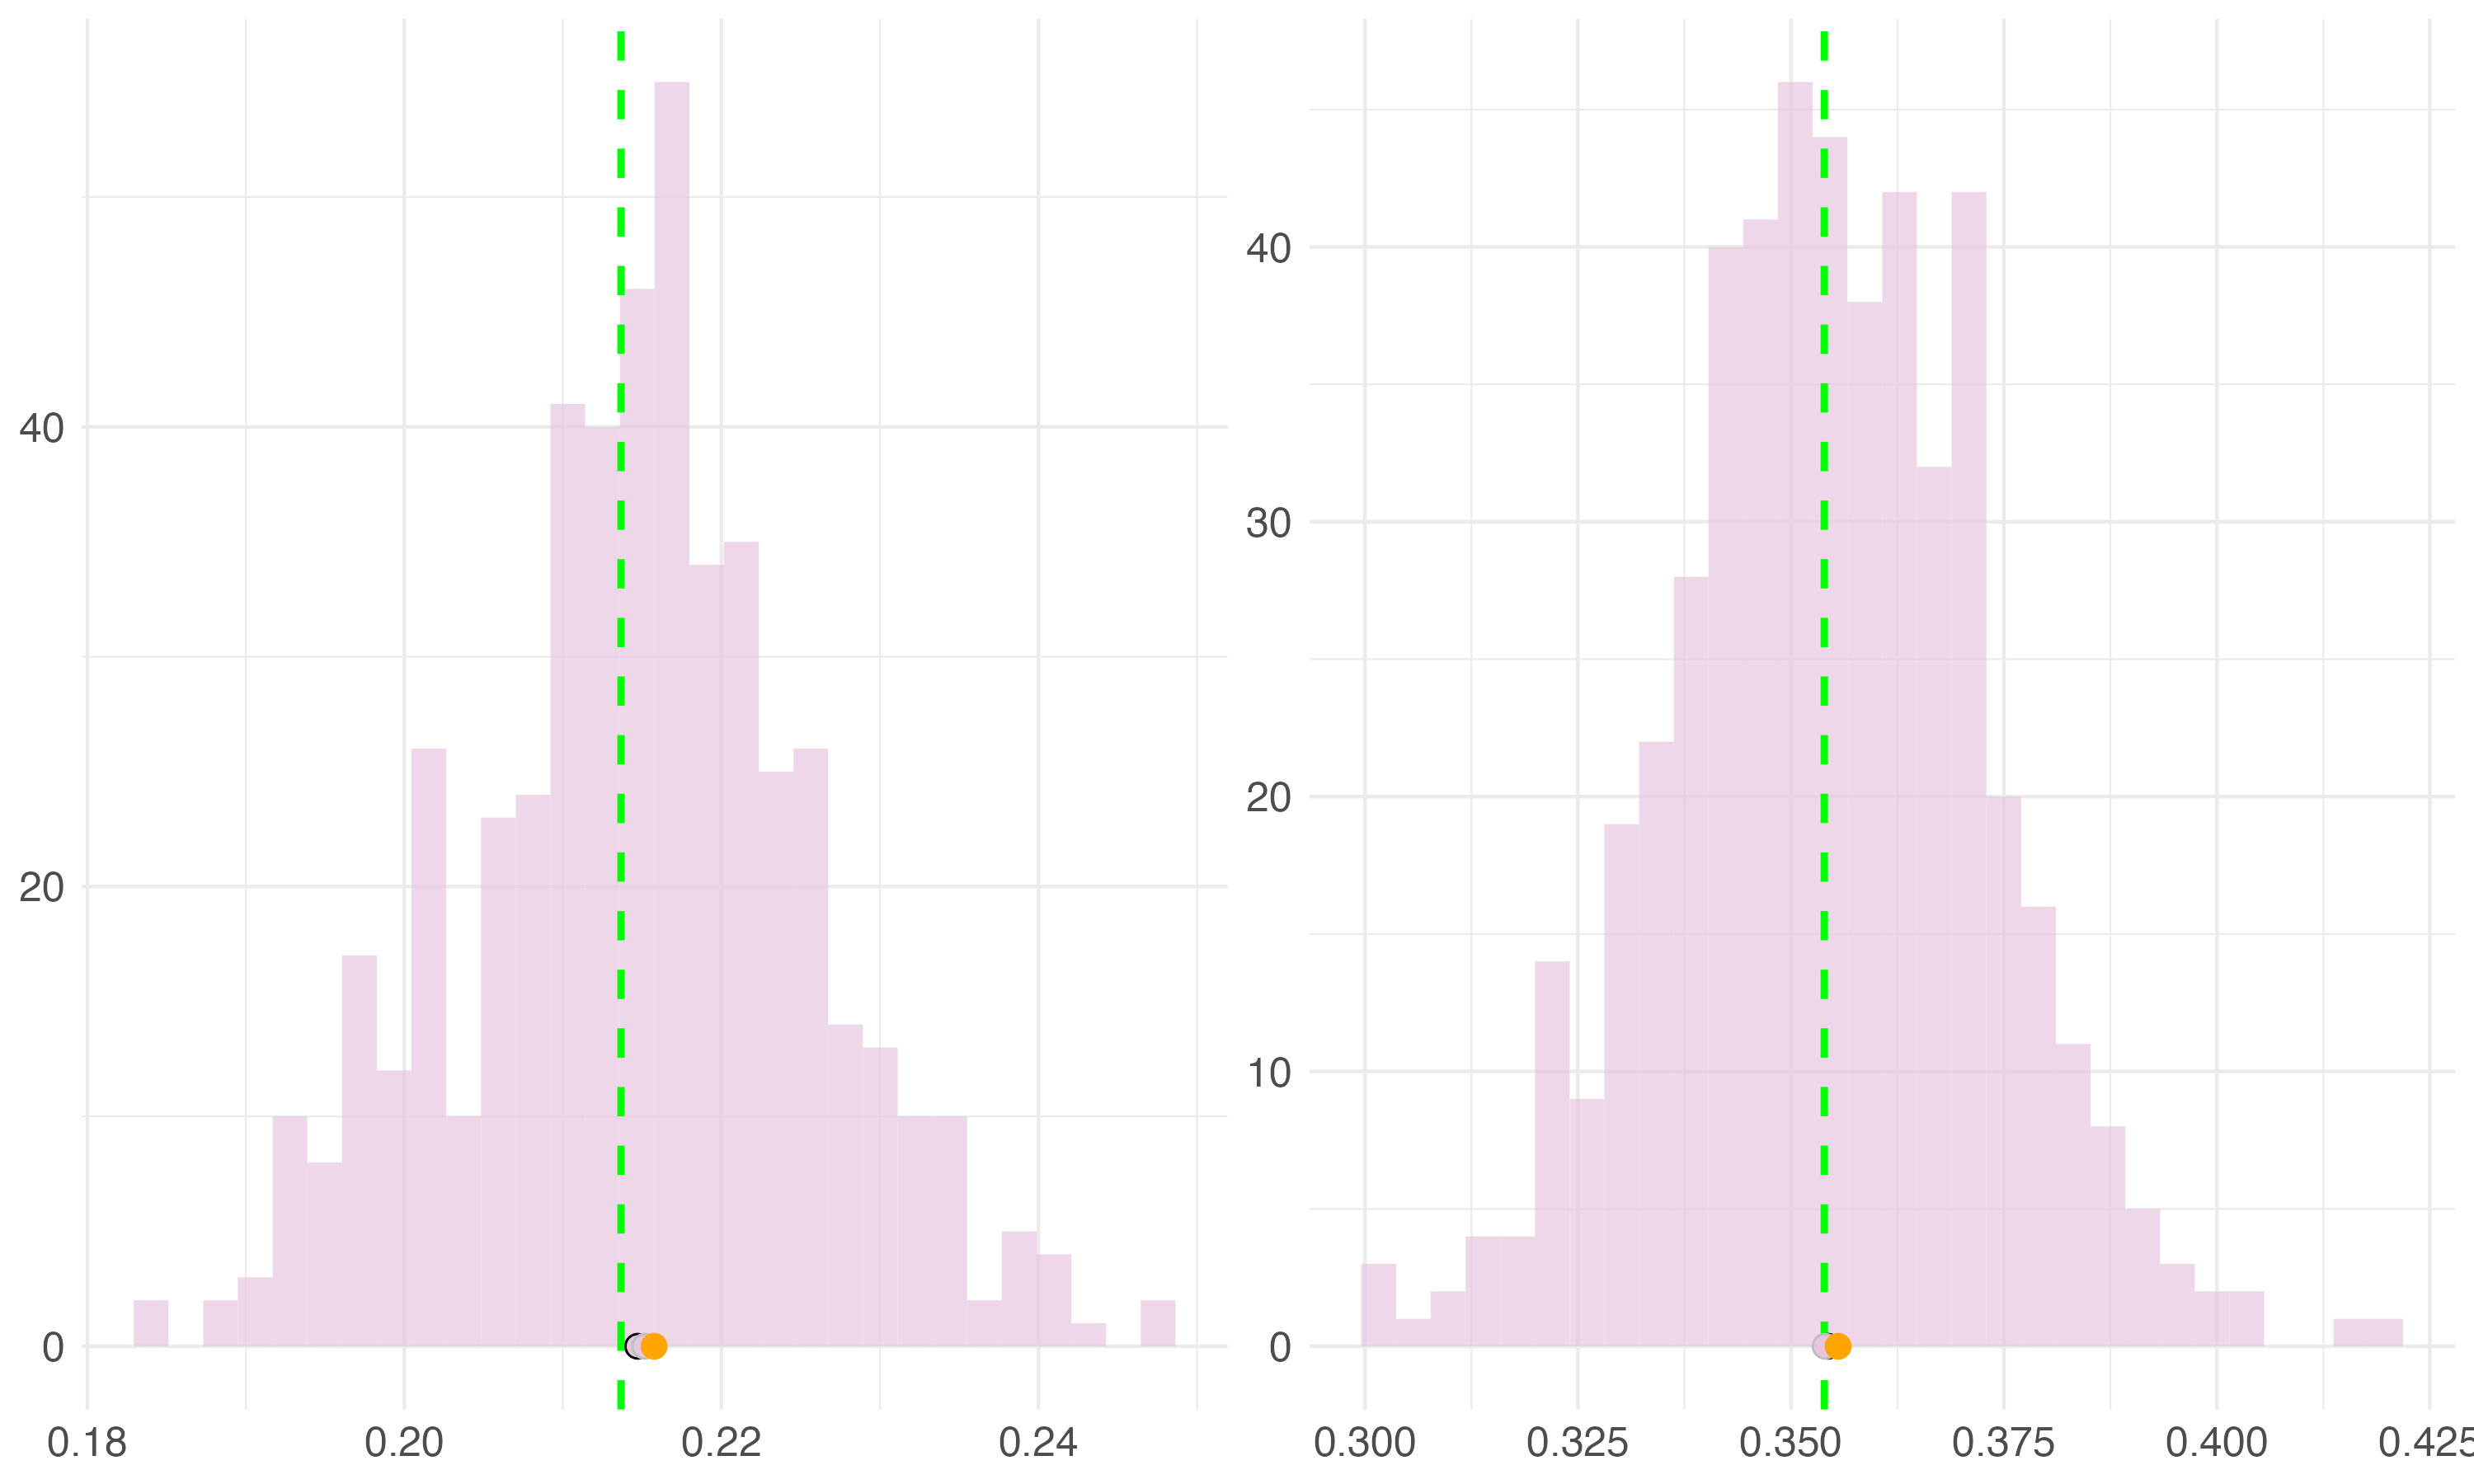
\includegraphics[width=1\linewidth]{Figures/Simulation study/R2_poisson_high_neg.png}
%   \caption{Histogram for the estimated marginal $R^2$ (left) and conditional $R^2$ (right) for the Poisson regression using the BVI method. The results are from the $N_{\text{sim}}=500$ simulations in the simulation study for different correlation levels $\rho$. The expected values are displayed as vertical green lines, and can be found in \Cref{table:r2values}. The mean value of the $R^2$ values for all simulations is marked with a circle at the bottom. (a) Marginal and conditional $R^2$ estimates for $\rho=-0.4$.}
%   \label{fig:r2_poisson_high_neg}
% \end{figure}
% \begin{figure}[H]\ContinuedFloat
%   \centering
%   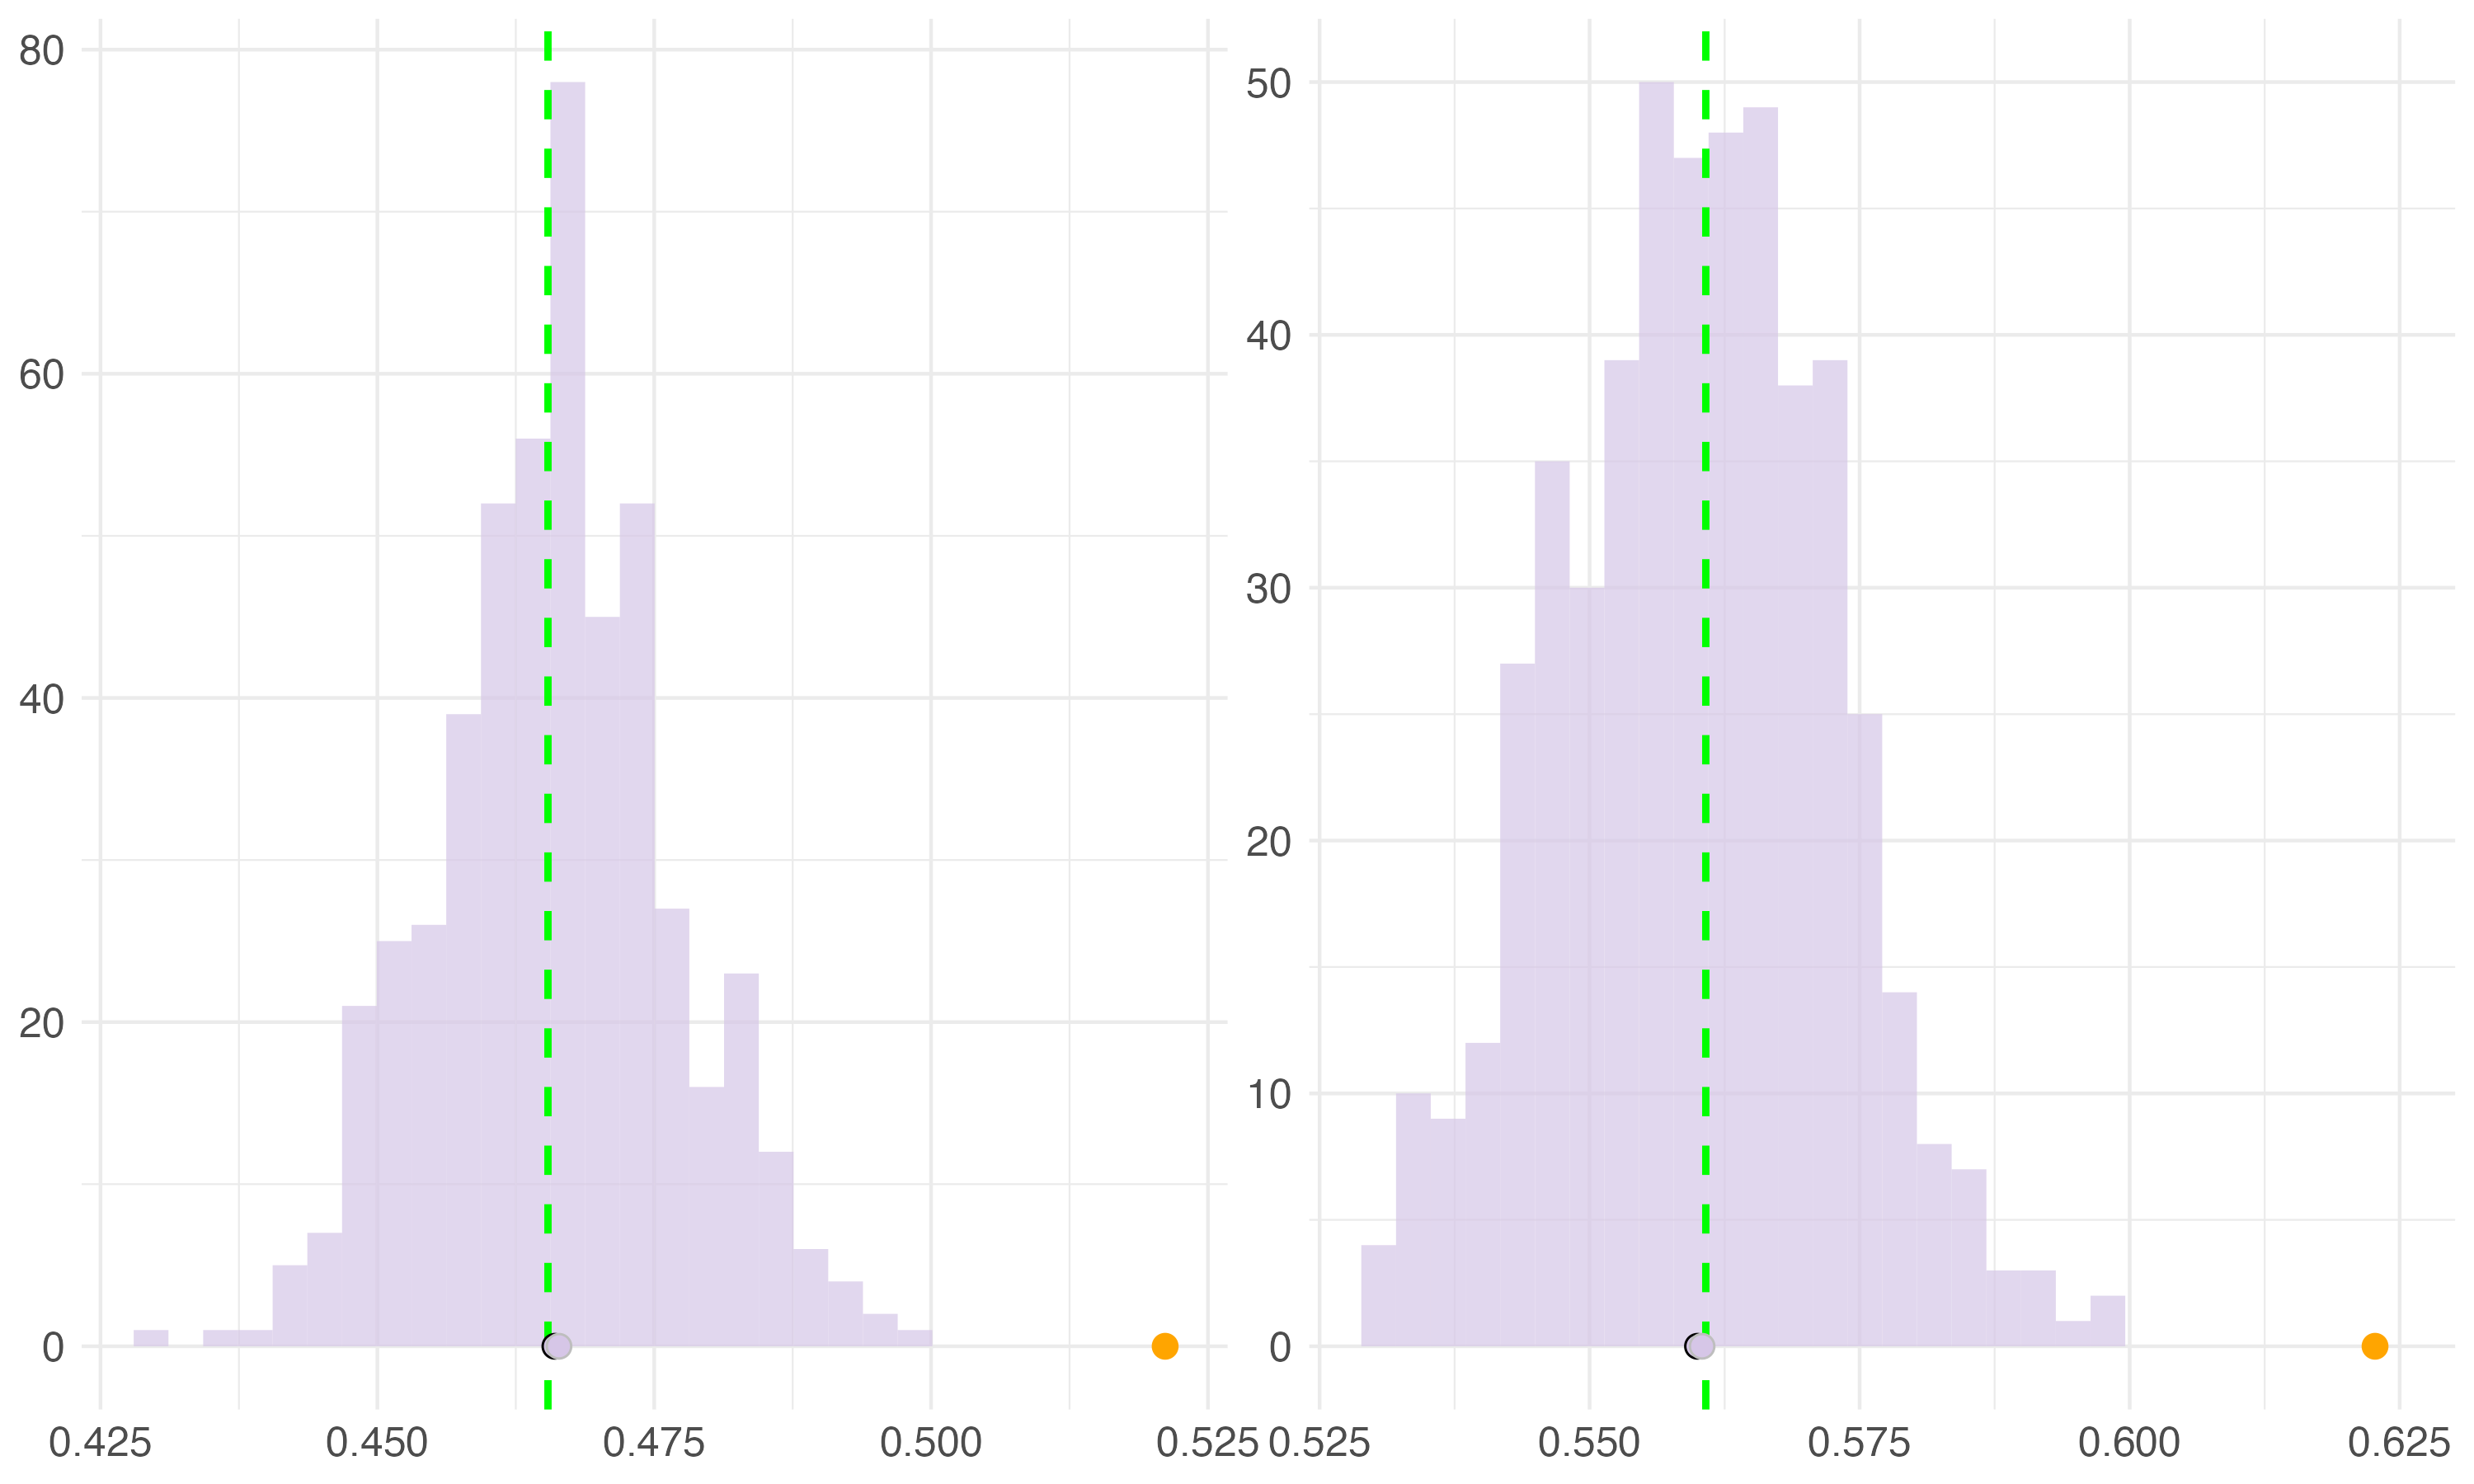
\includegraphics[width=1\linewidth]{Figures/Simulation study/R2_poisson_low_neg.png}
%   \caption{(b) Marginal and conditional $R^2$ estimates for $\rho=-0.1$.}
%   \label{fig:r2_poisson_low_neg}
% \end{figure}
% \begin{figure}[H]\ContinuedFloat
%   \centering
%   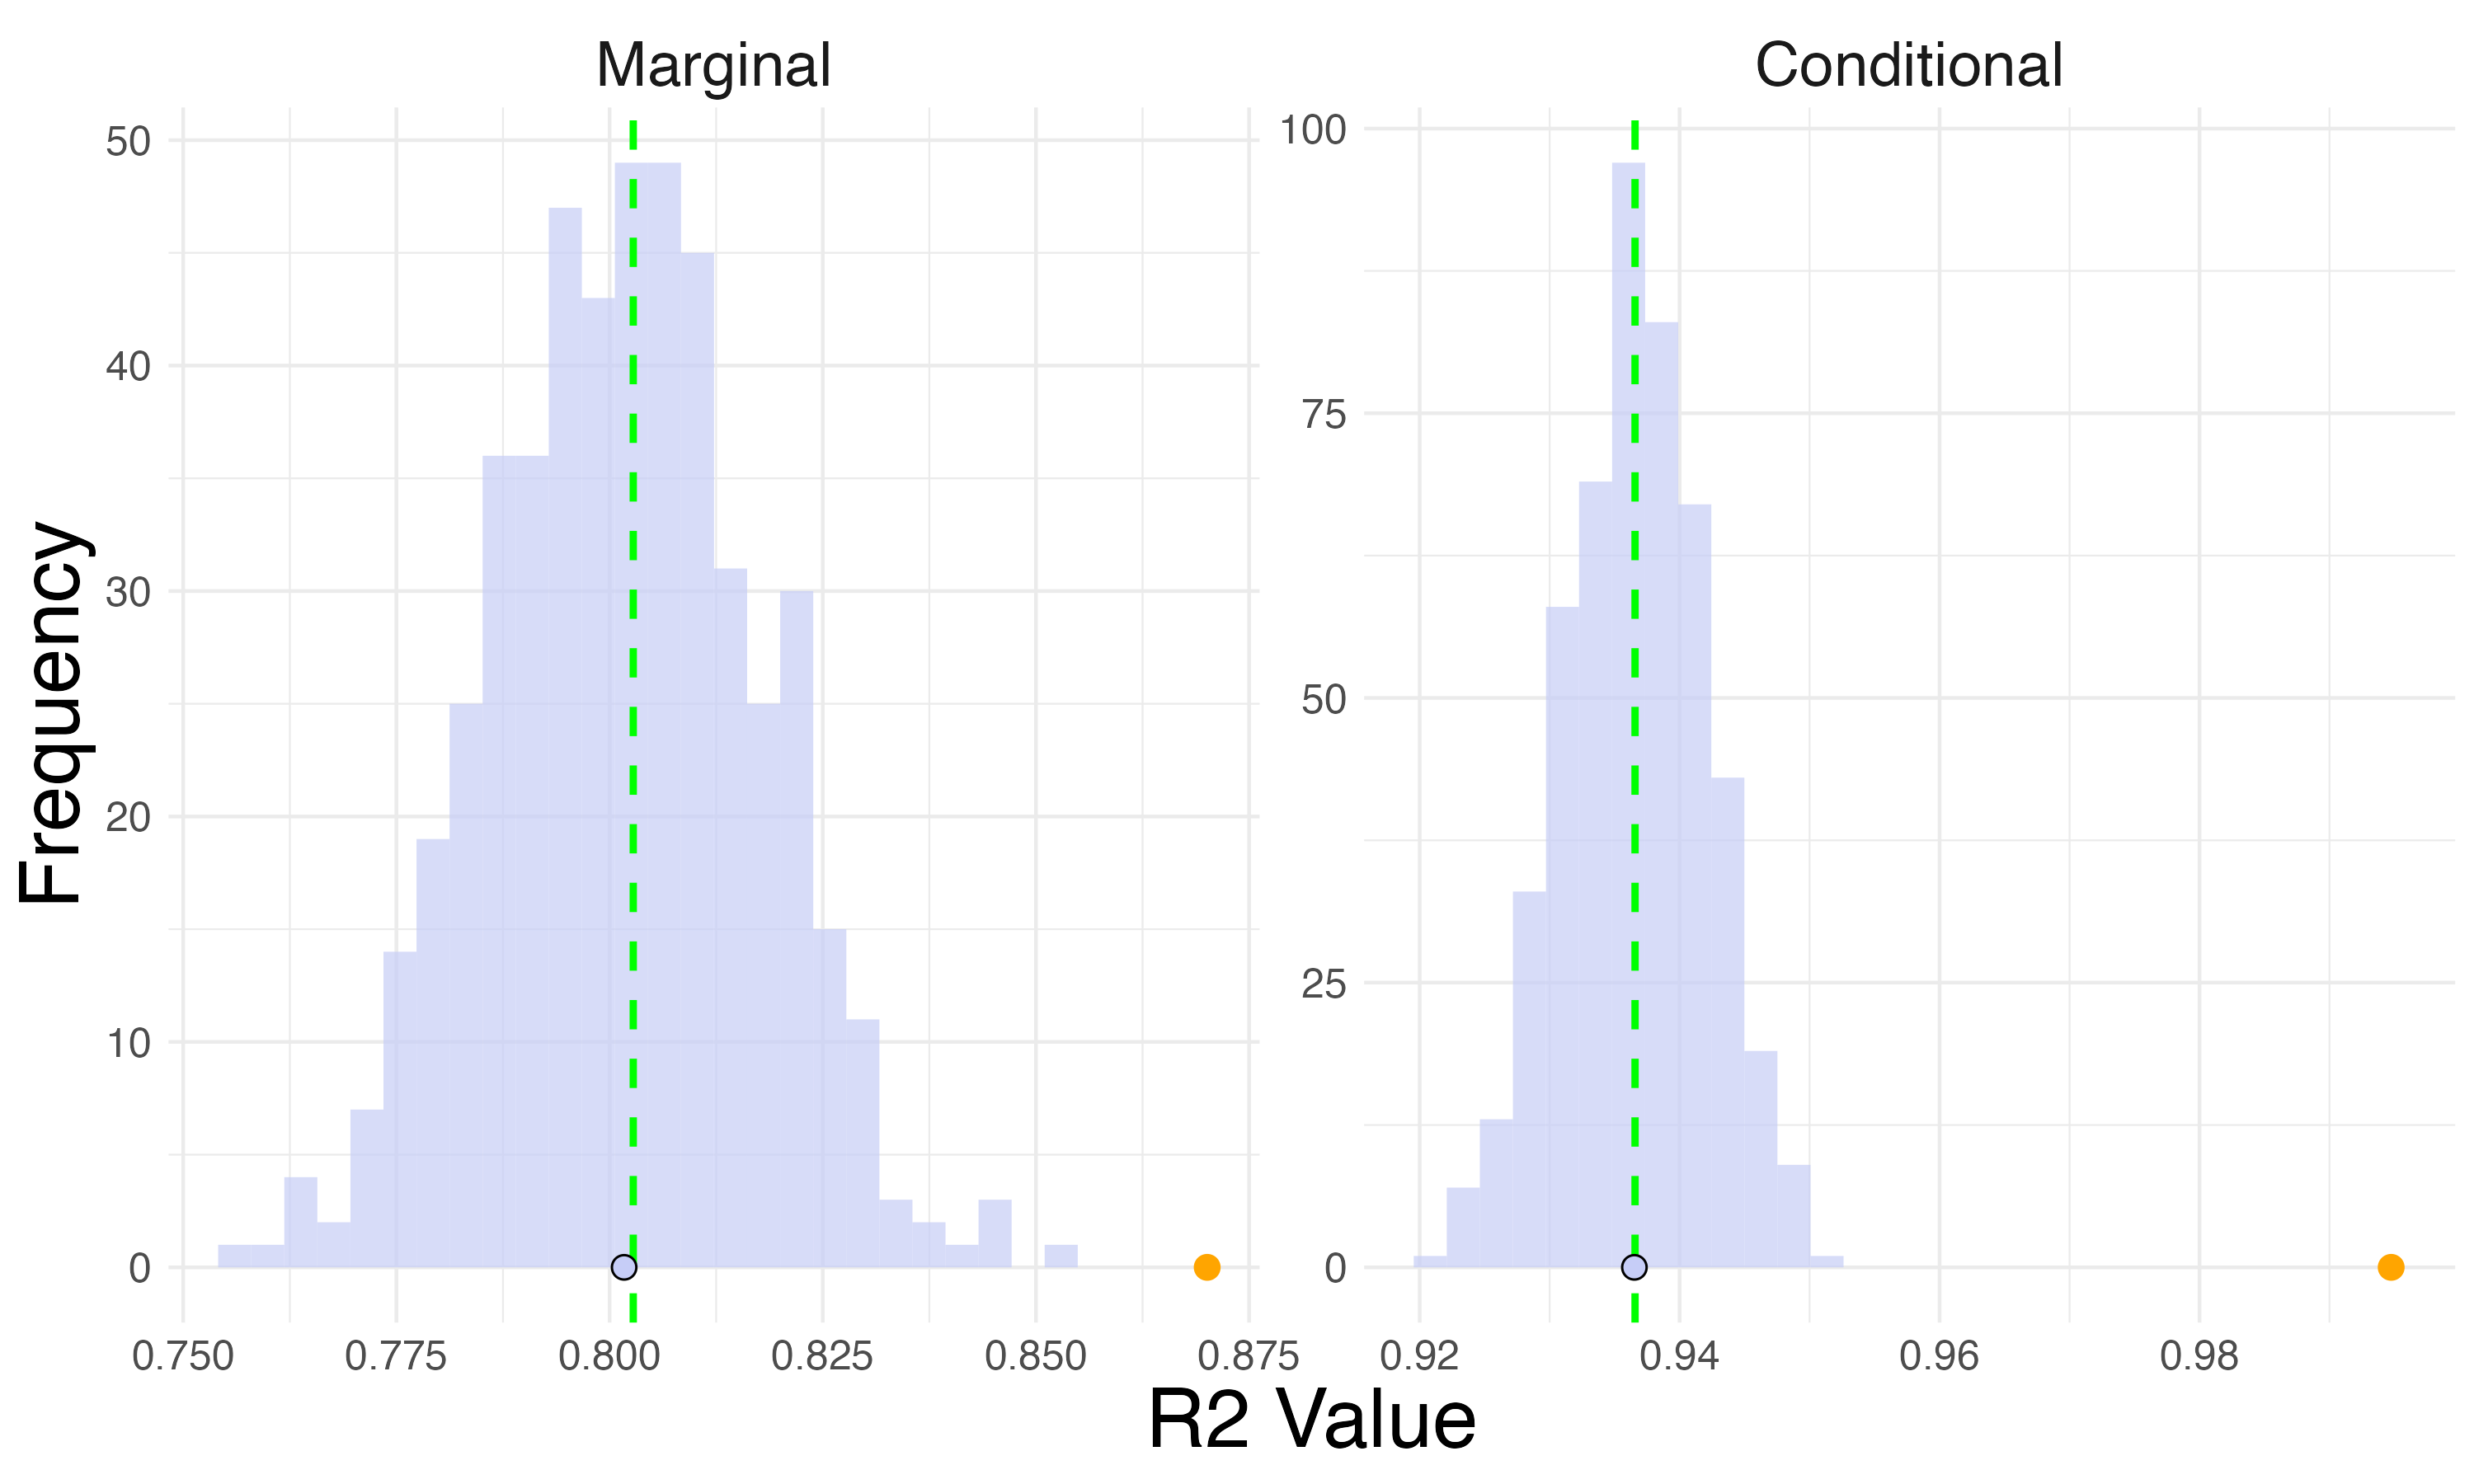
\includegraphics[width=1\linewidth]{Figures/Simulation study/R2_poisson_no.png}
%   \caption{(c) Marginal and conditional $R^2$ estimates for $\rho=0$.}
%   \label{fig:r2_poisson_no}
% \end{figure}
% \begin{figure}[H]\ContinuedFloat
%   \centering
%   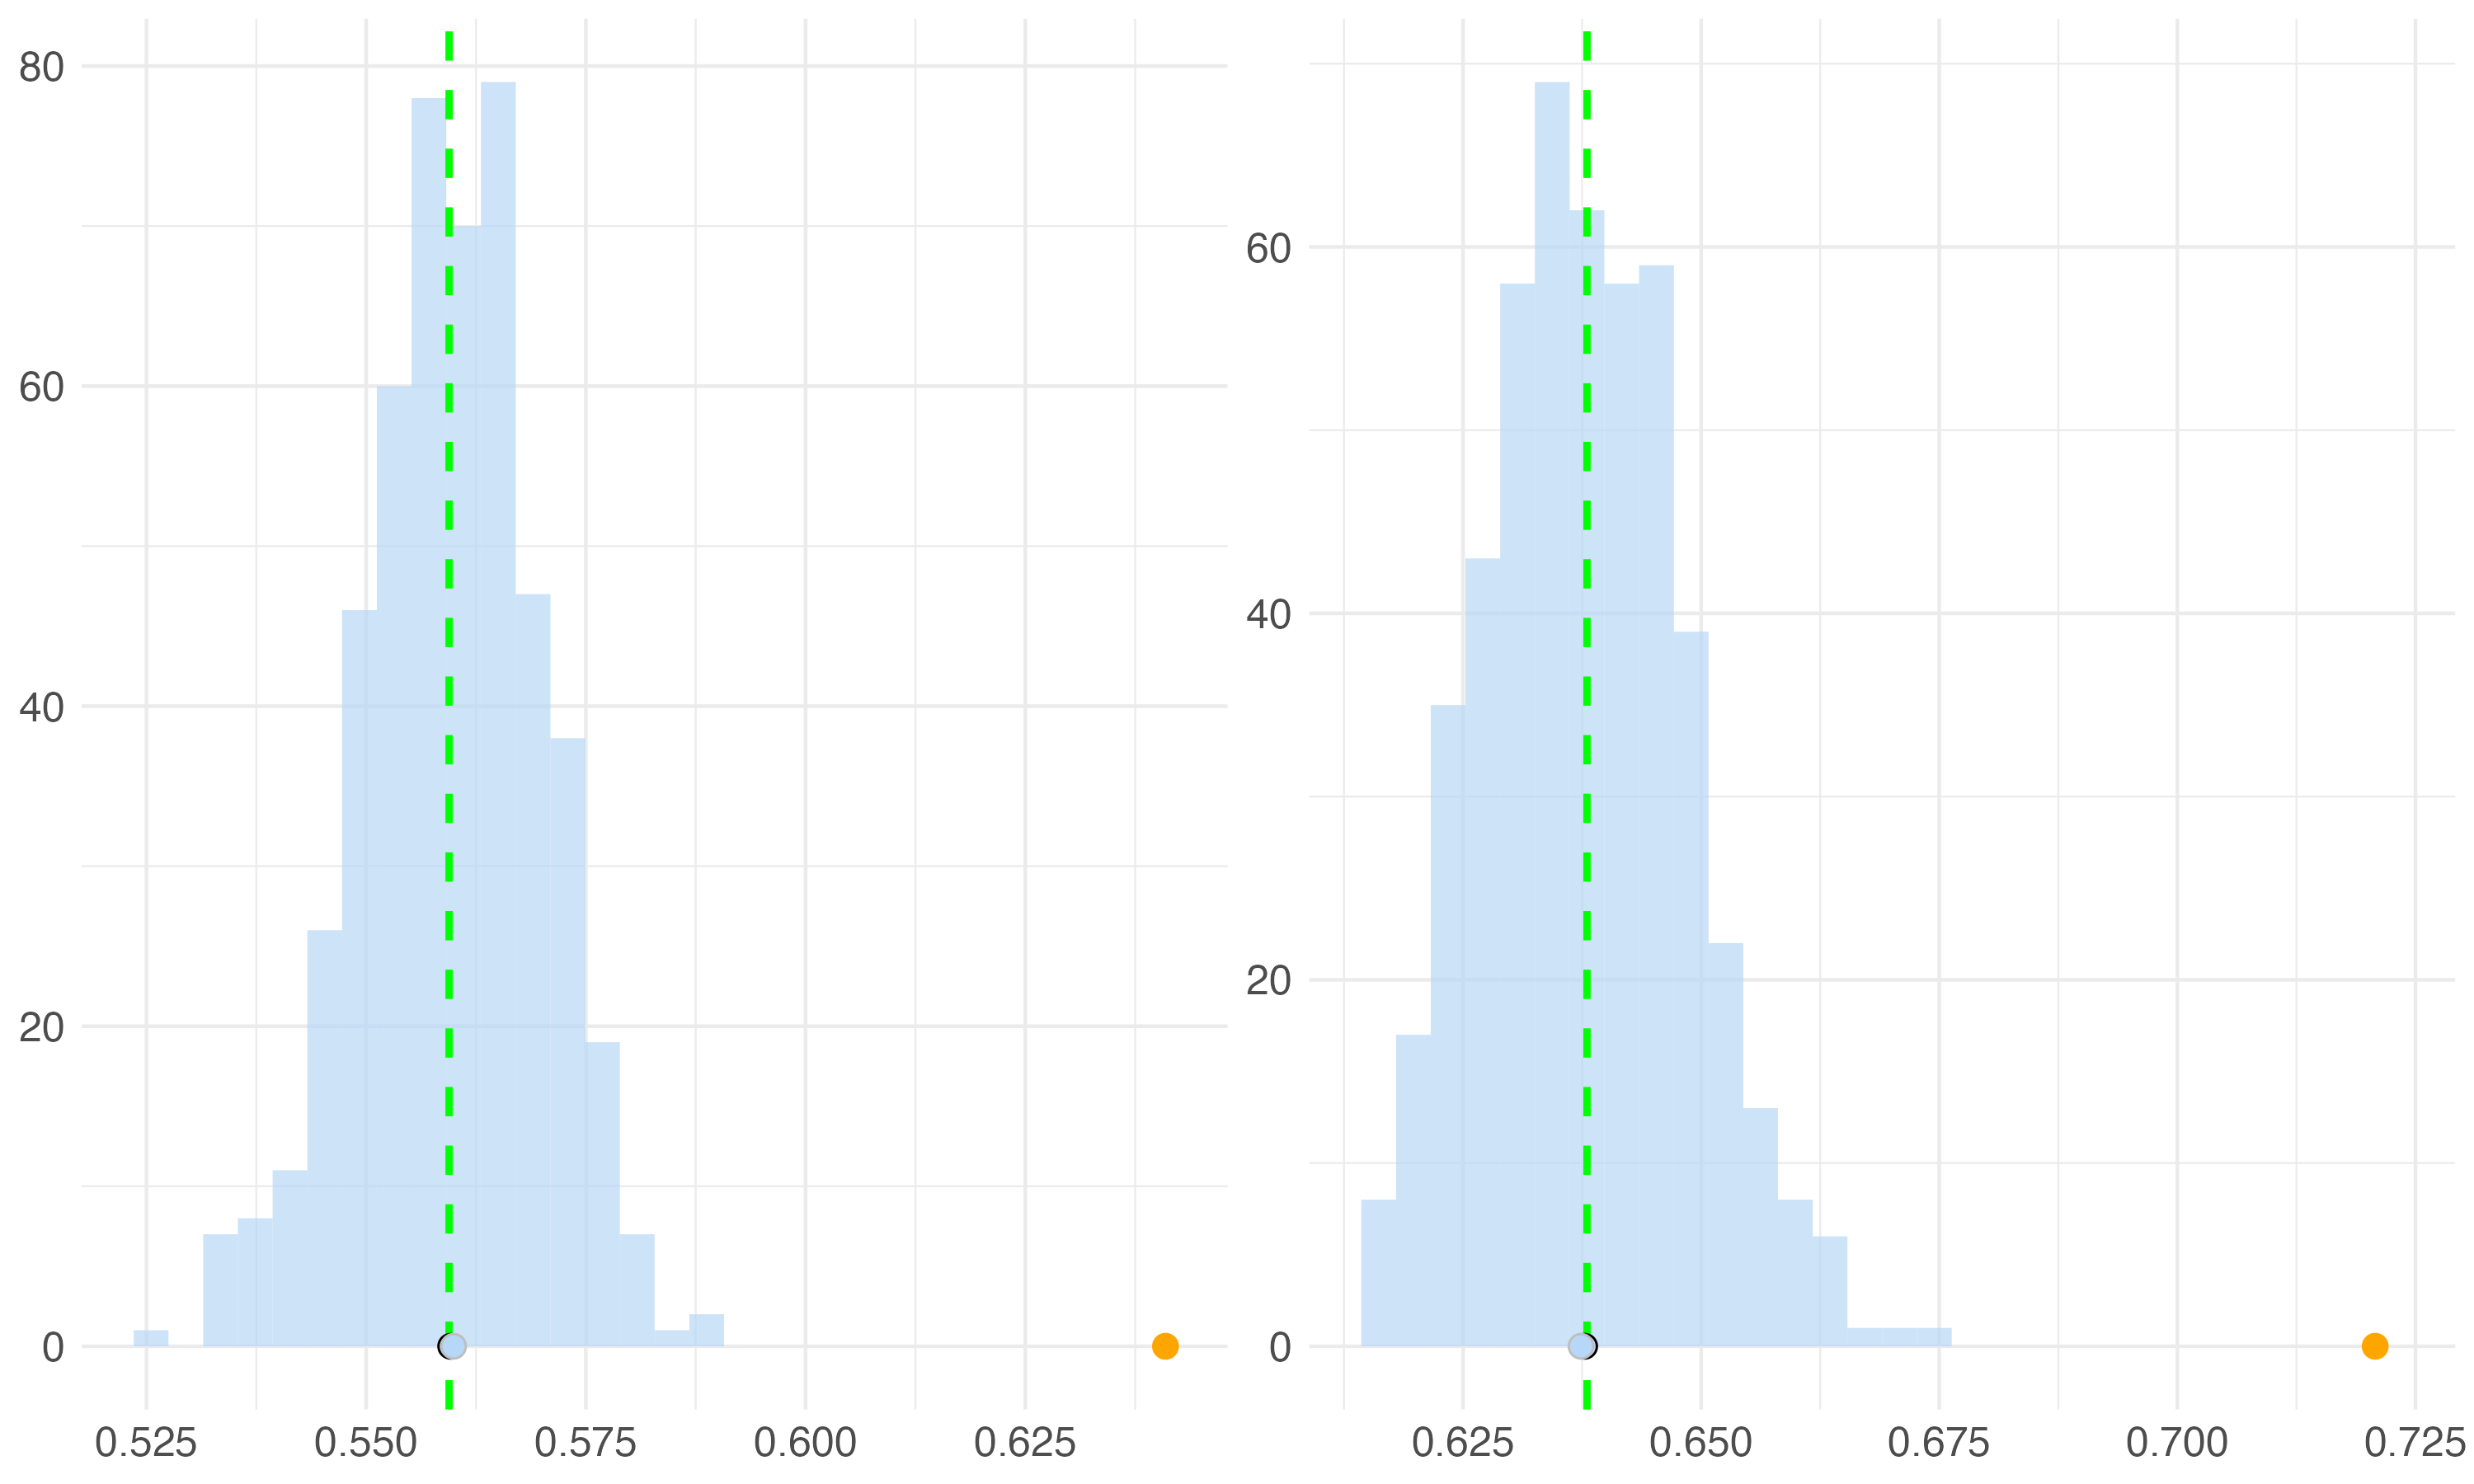
\includegraphics[width=1\linewidth]{Figures/Simulation study/R2_poisson_low_pos.png}
%   \caption{(d) Marginal and conditional $R^2$ estimates for $\rho=0.1$.}
%   \label{fig:r2_poisson_low_pos}
% \end{figure}
% \begin{figure}[H]\ContinuedFloat
%   \centering
%   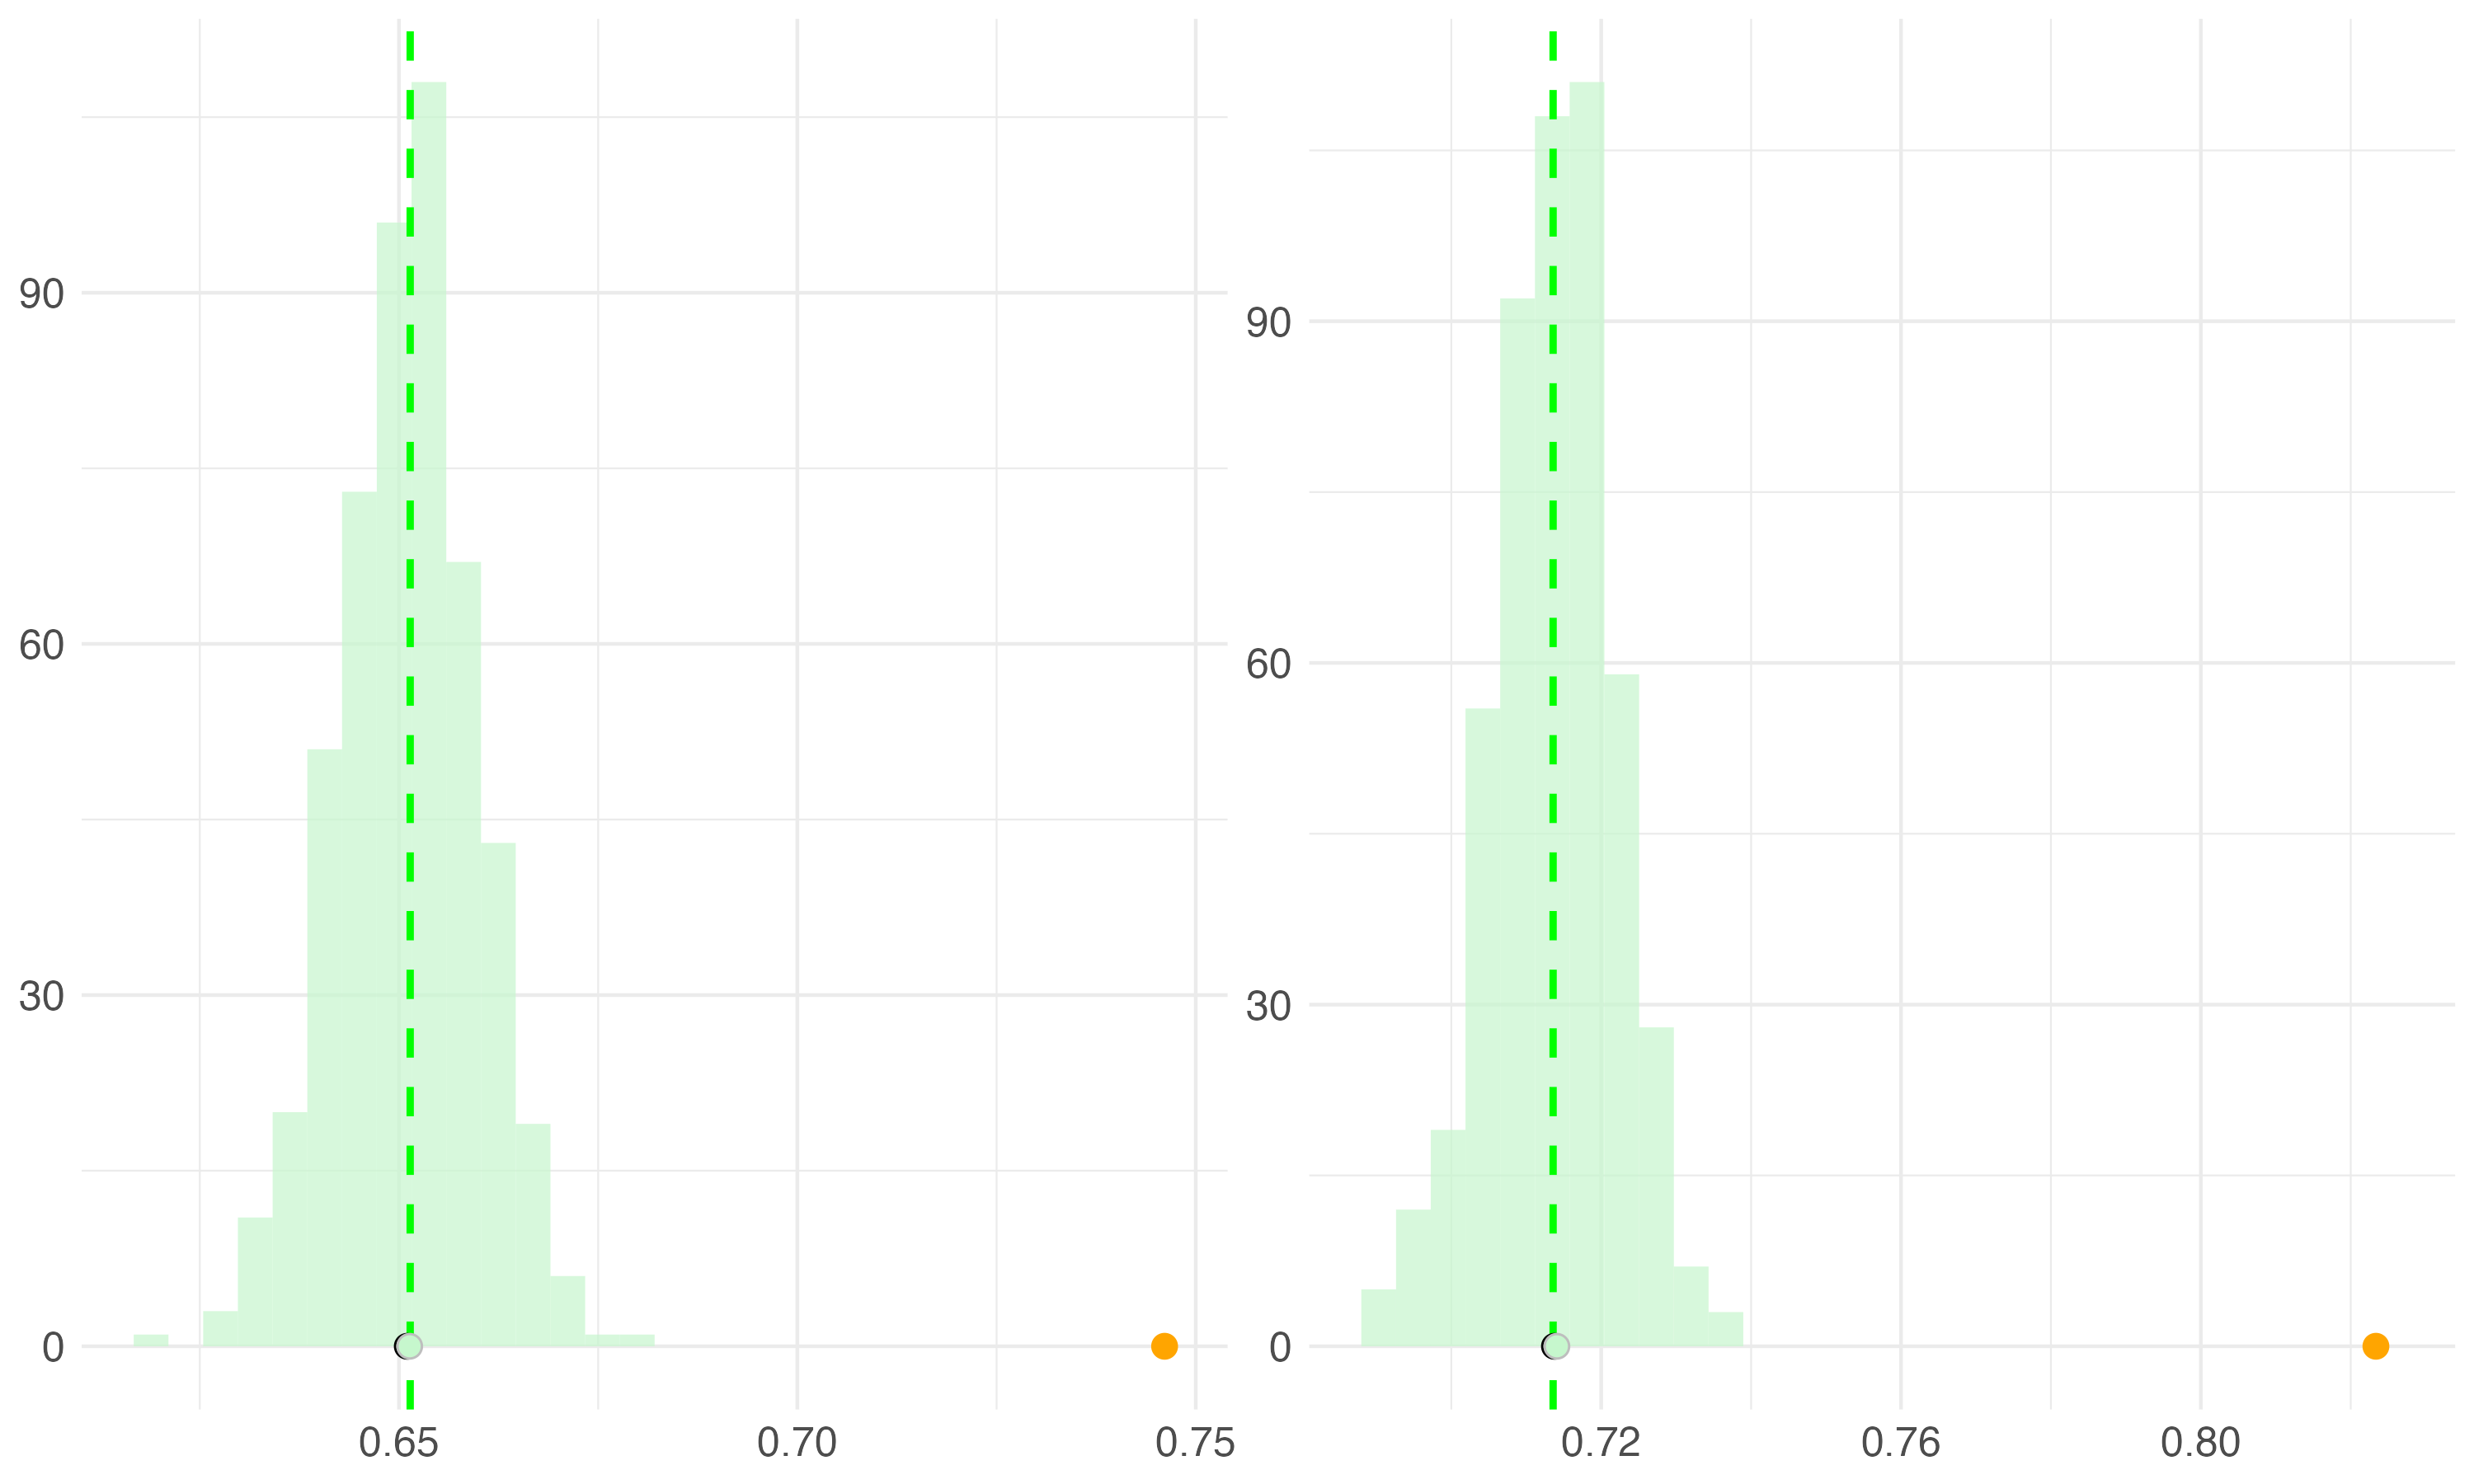
\includegraphics[width=1\linewidth]{Figures/Simulation study/R2_poisson_high_pos.png}
%   \caption{(e) Marginal and conditional $R^2$ estimates for $\rho=0.4$.}
%   \label{fig:r2_poisson_high_pos}
% \end{figure}

\begin{figure}[H]
  \centering
  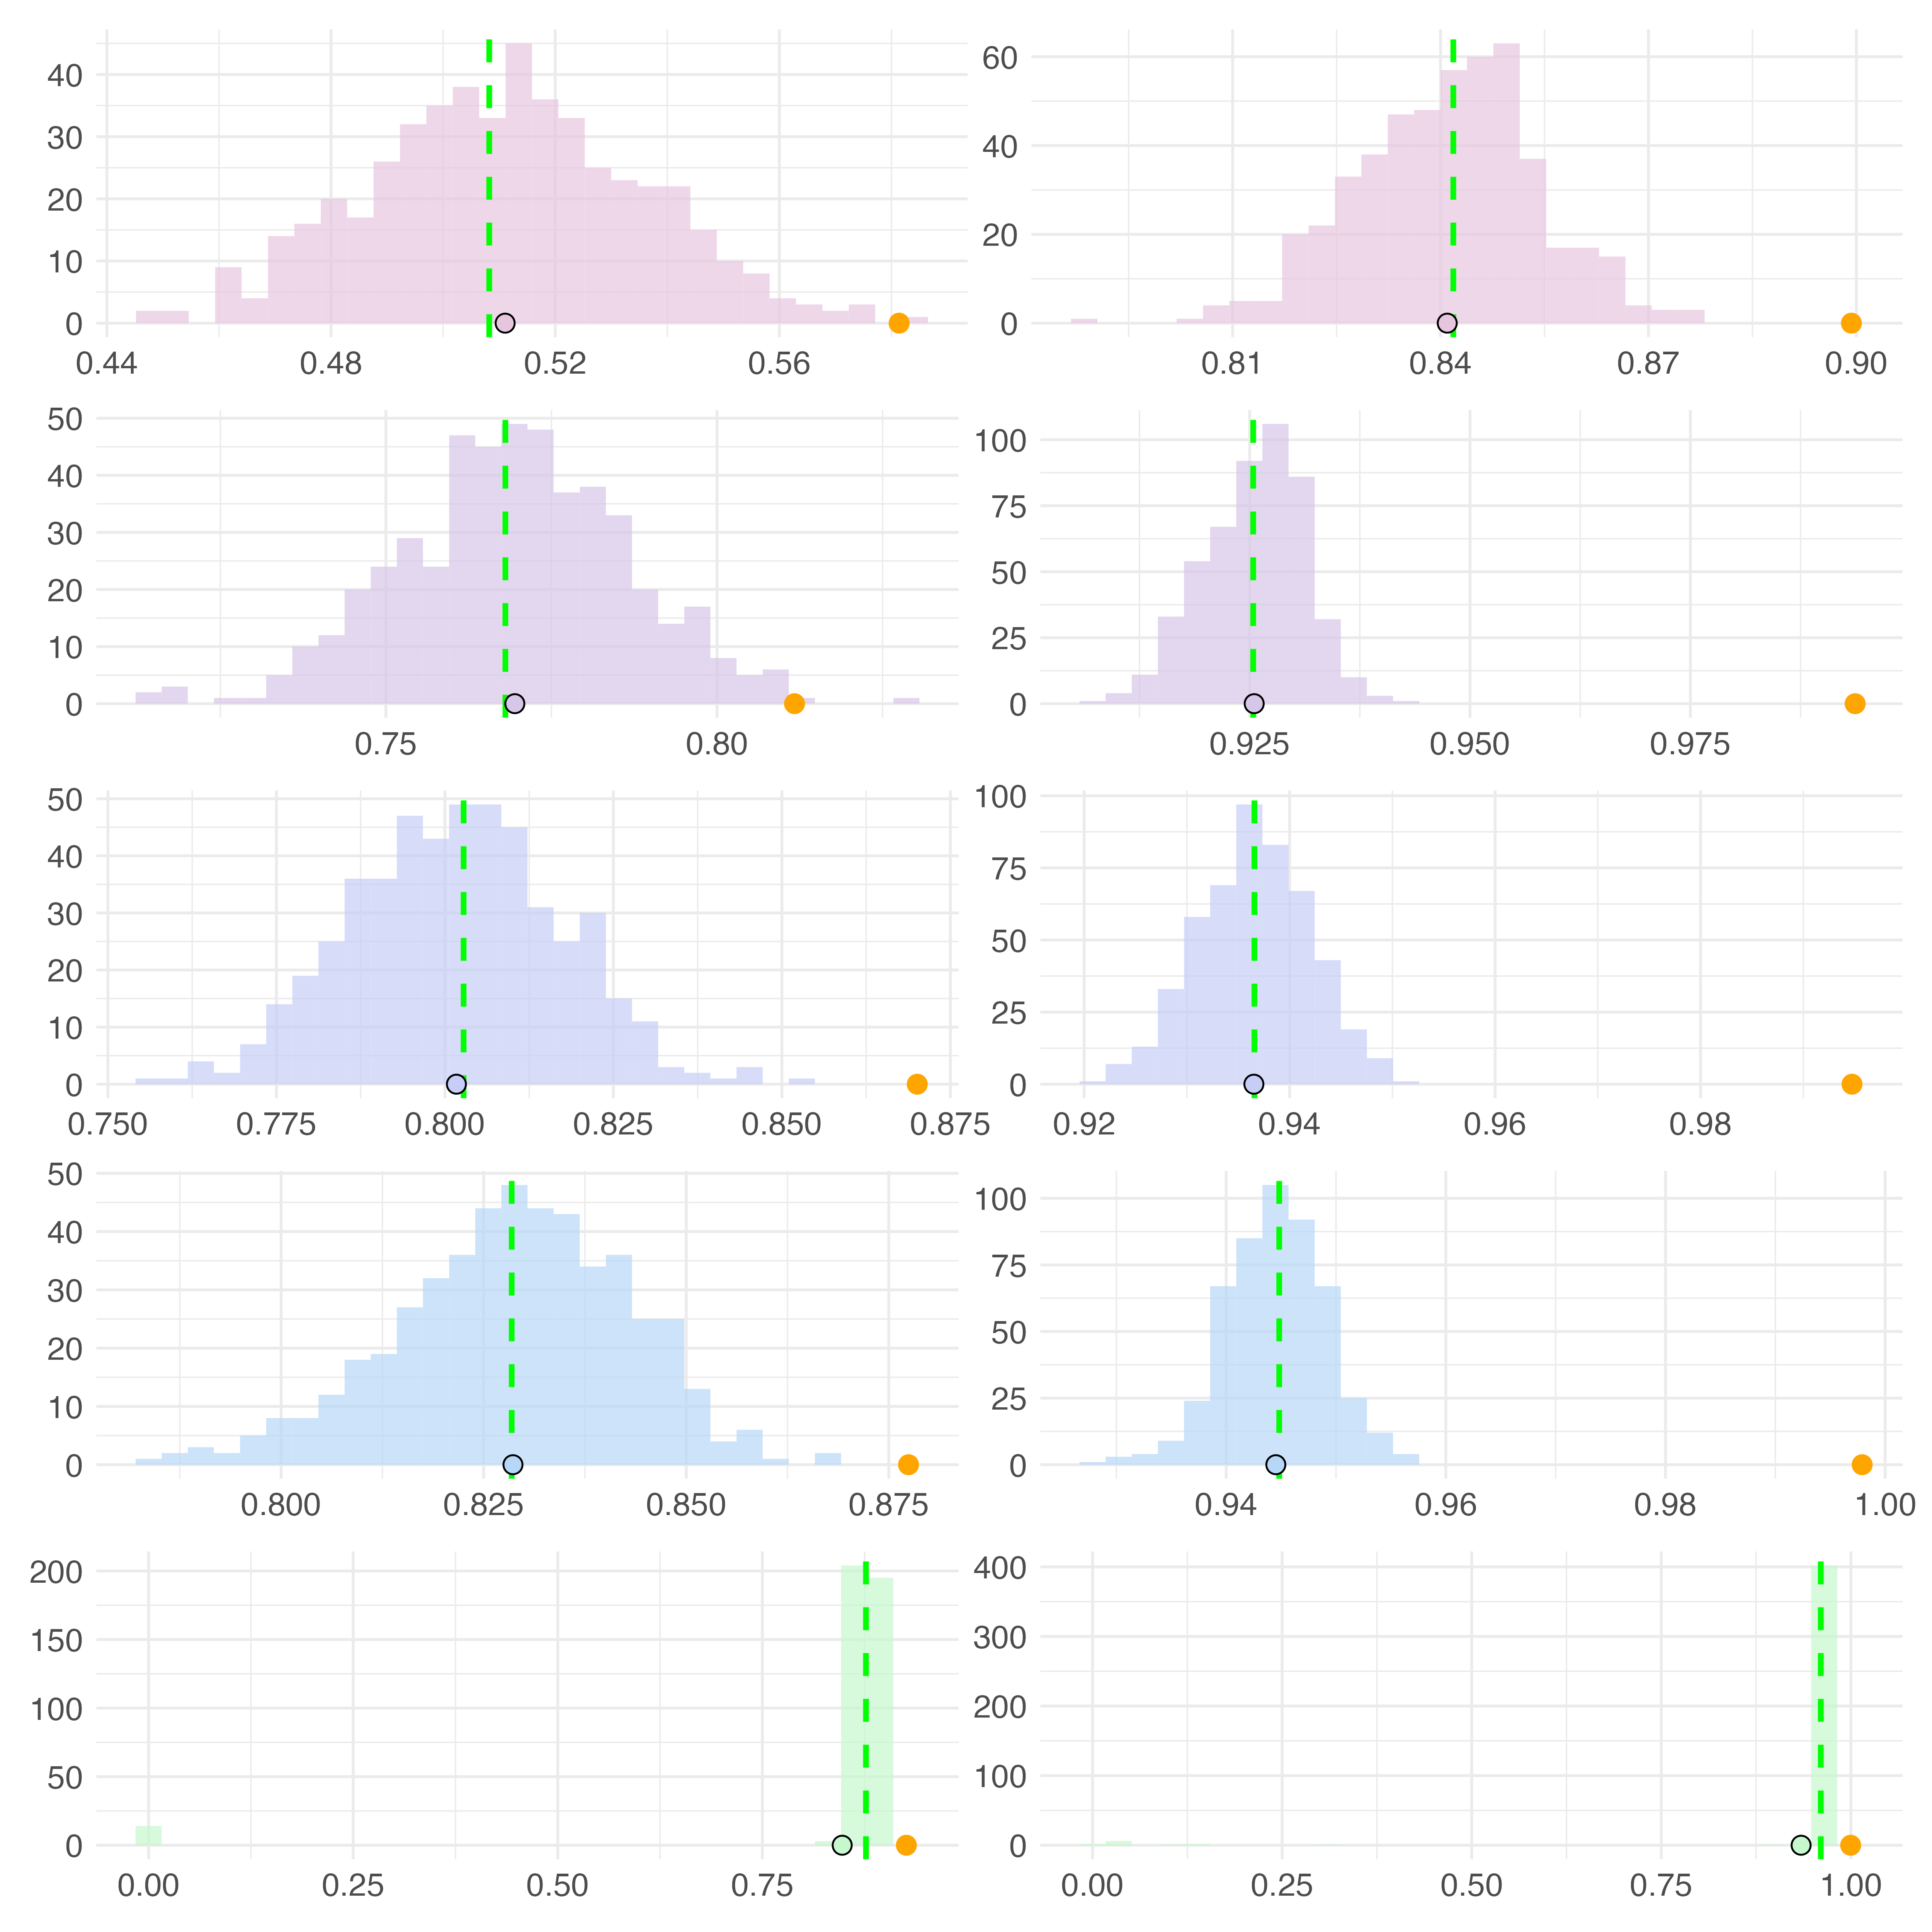
\includegraphics[width=1.1\linewidth]{Figures/Simulation study/R2_combined_poisson.png}
  \caption{Histograms with the estimated marginal $R^2$ (left) and conditional $R^2$ (right) from the BVI method for the binomial regression for the different correlation levels $\rho=-0.4$ (top), $\rho=-0.1$ (second from the top), $\rho=0$ (middle), $\rho=0.1$ (second from bottom) and $\rho=0.4$ (bottom). The values are calculated by the Bayesian Variable Importance method from the $N_{\text{sim}}=500$ simulations in the simulation study. The expected values are displayed as vertical green lines, and can be found in \Cref{table:r2values}, while the orange dot denotes the estimate from the \texttt{rptR} package. The mean value of the $R^2$ values for all simulations is marked with a circle at the bottom of each histogram.}
  \label{fig:r2_combined_poisson}
\end{figure}


% \begin{figure}[H]
%   \centering
%     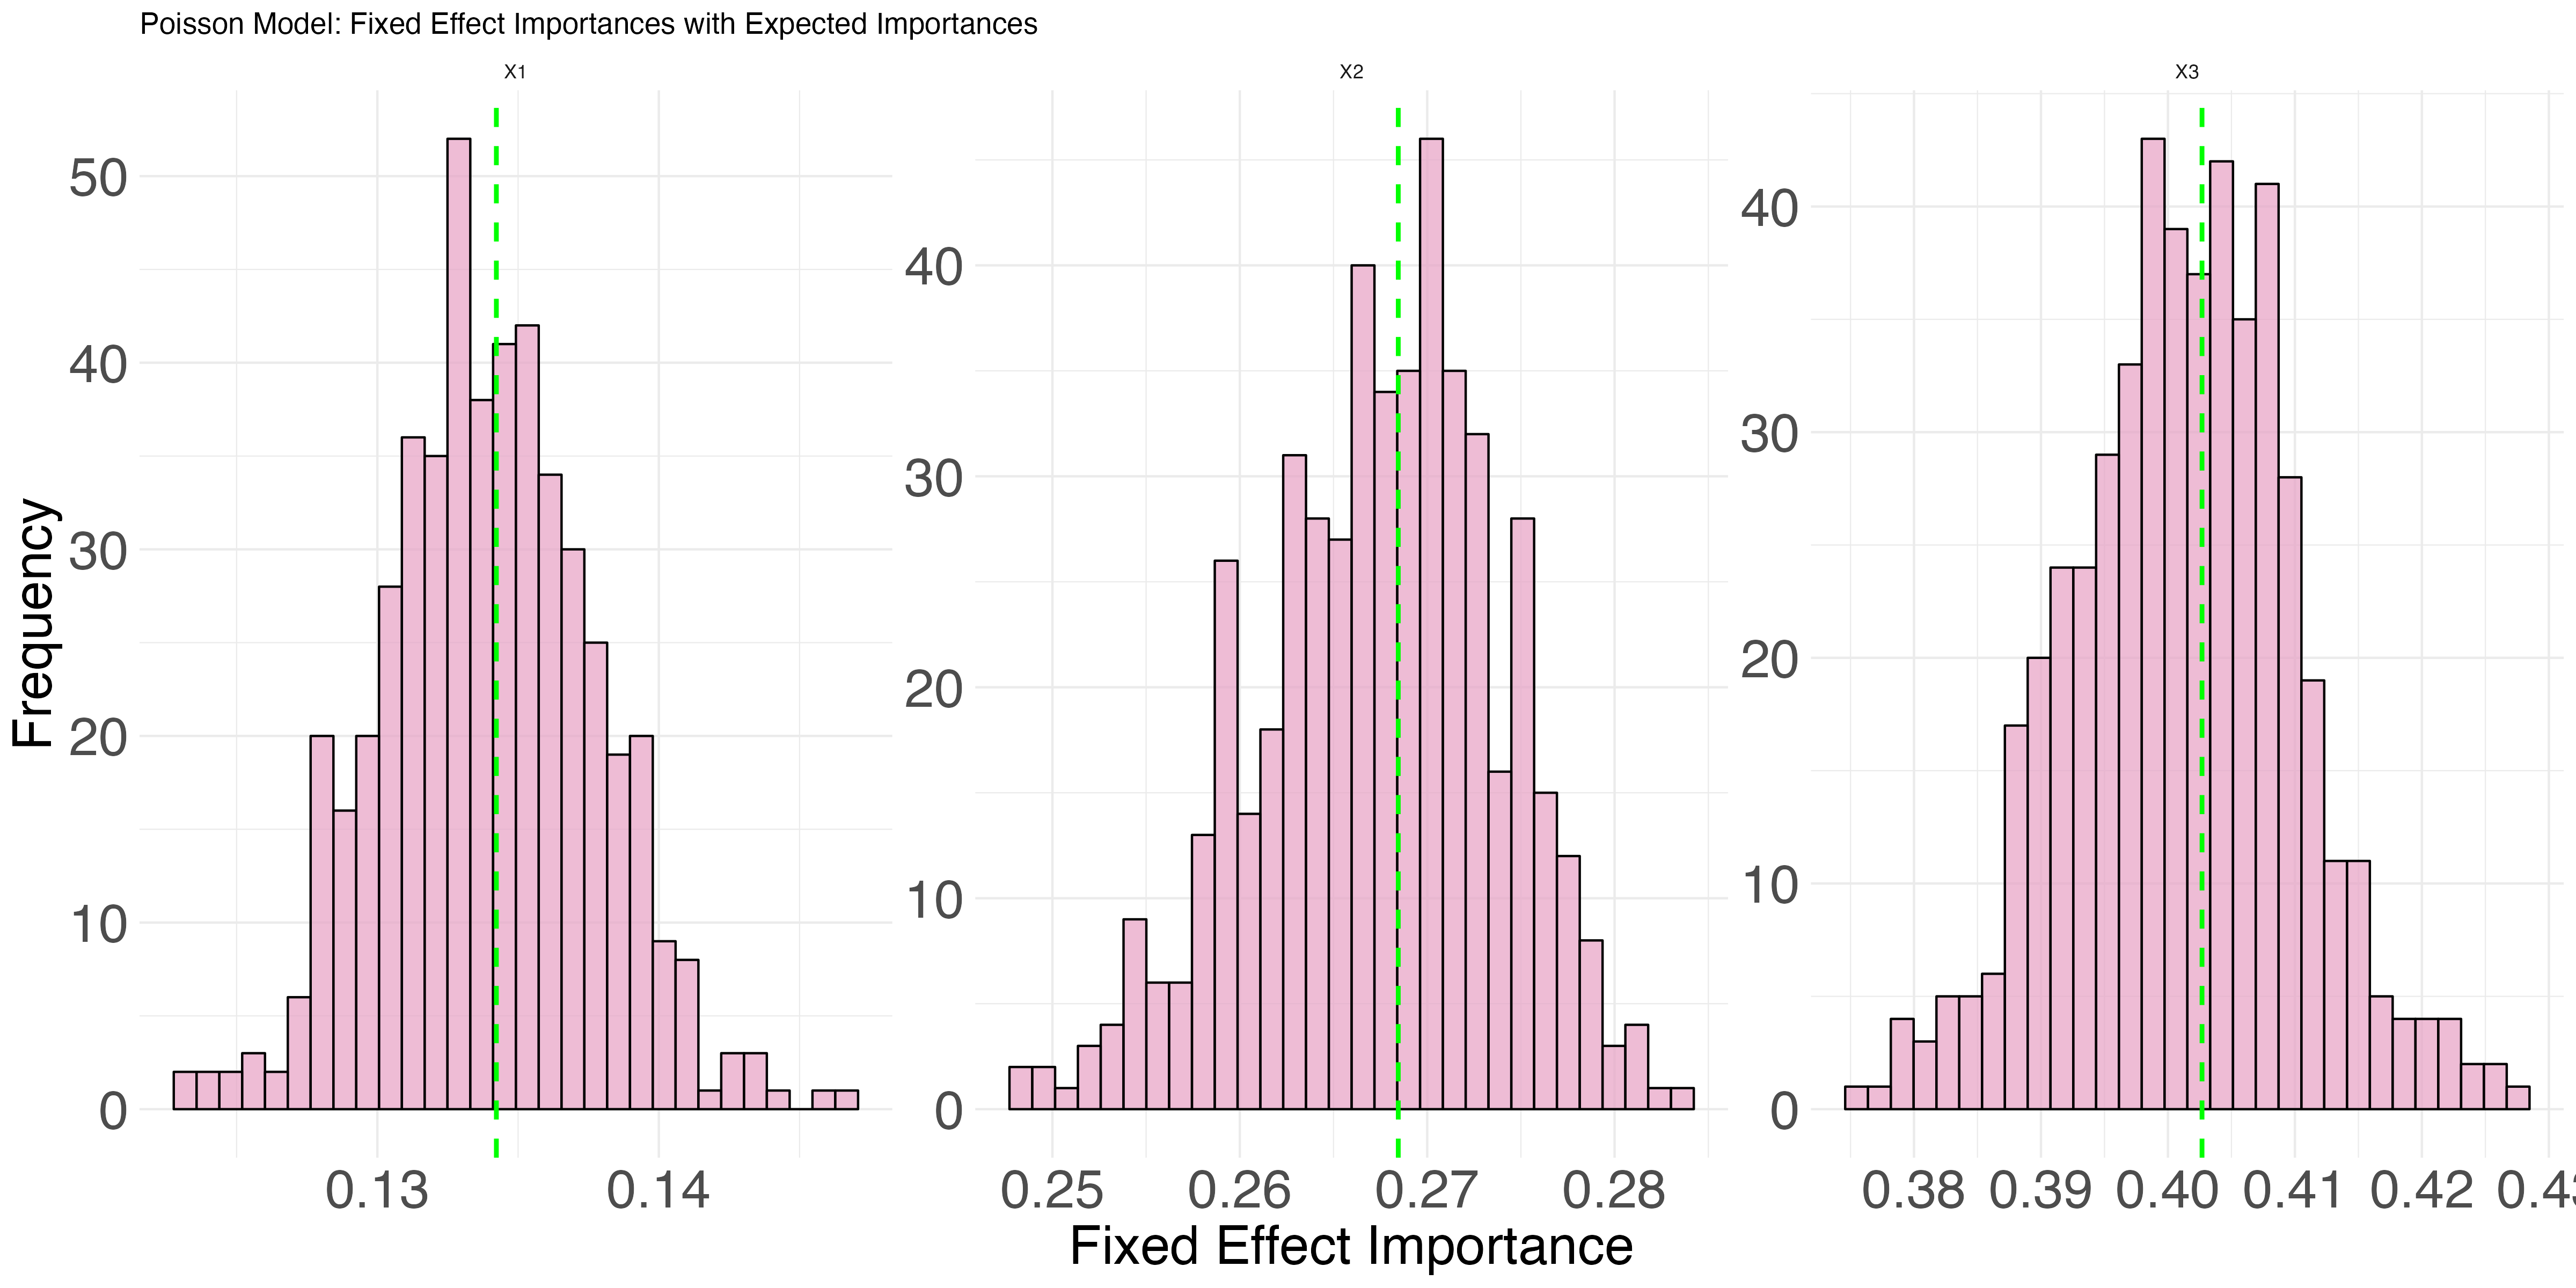
\includegraphics[width=1\linewidth]{Figures/Simulation study/Fixed_poisson.png}
%     \caption{Relative importance of fixed effects for poisson GLMM}
%     \label{fig:relimp_poisson_fixed}
% \end{figure}
% \begin{figure}[H]\ContinuedFloat
%   \centering
%   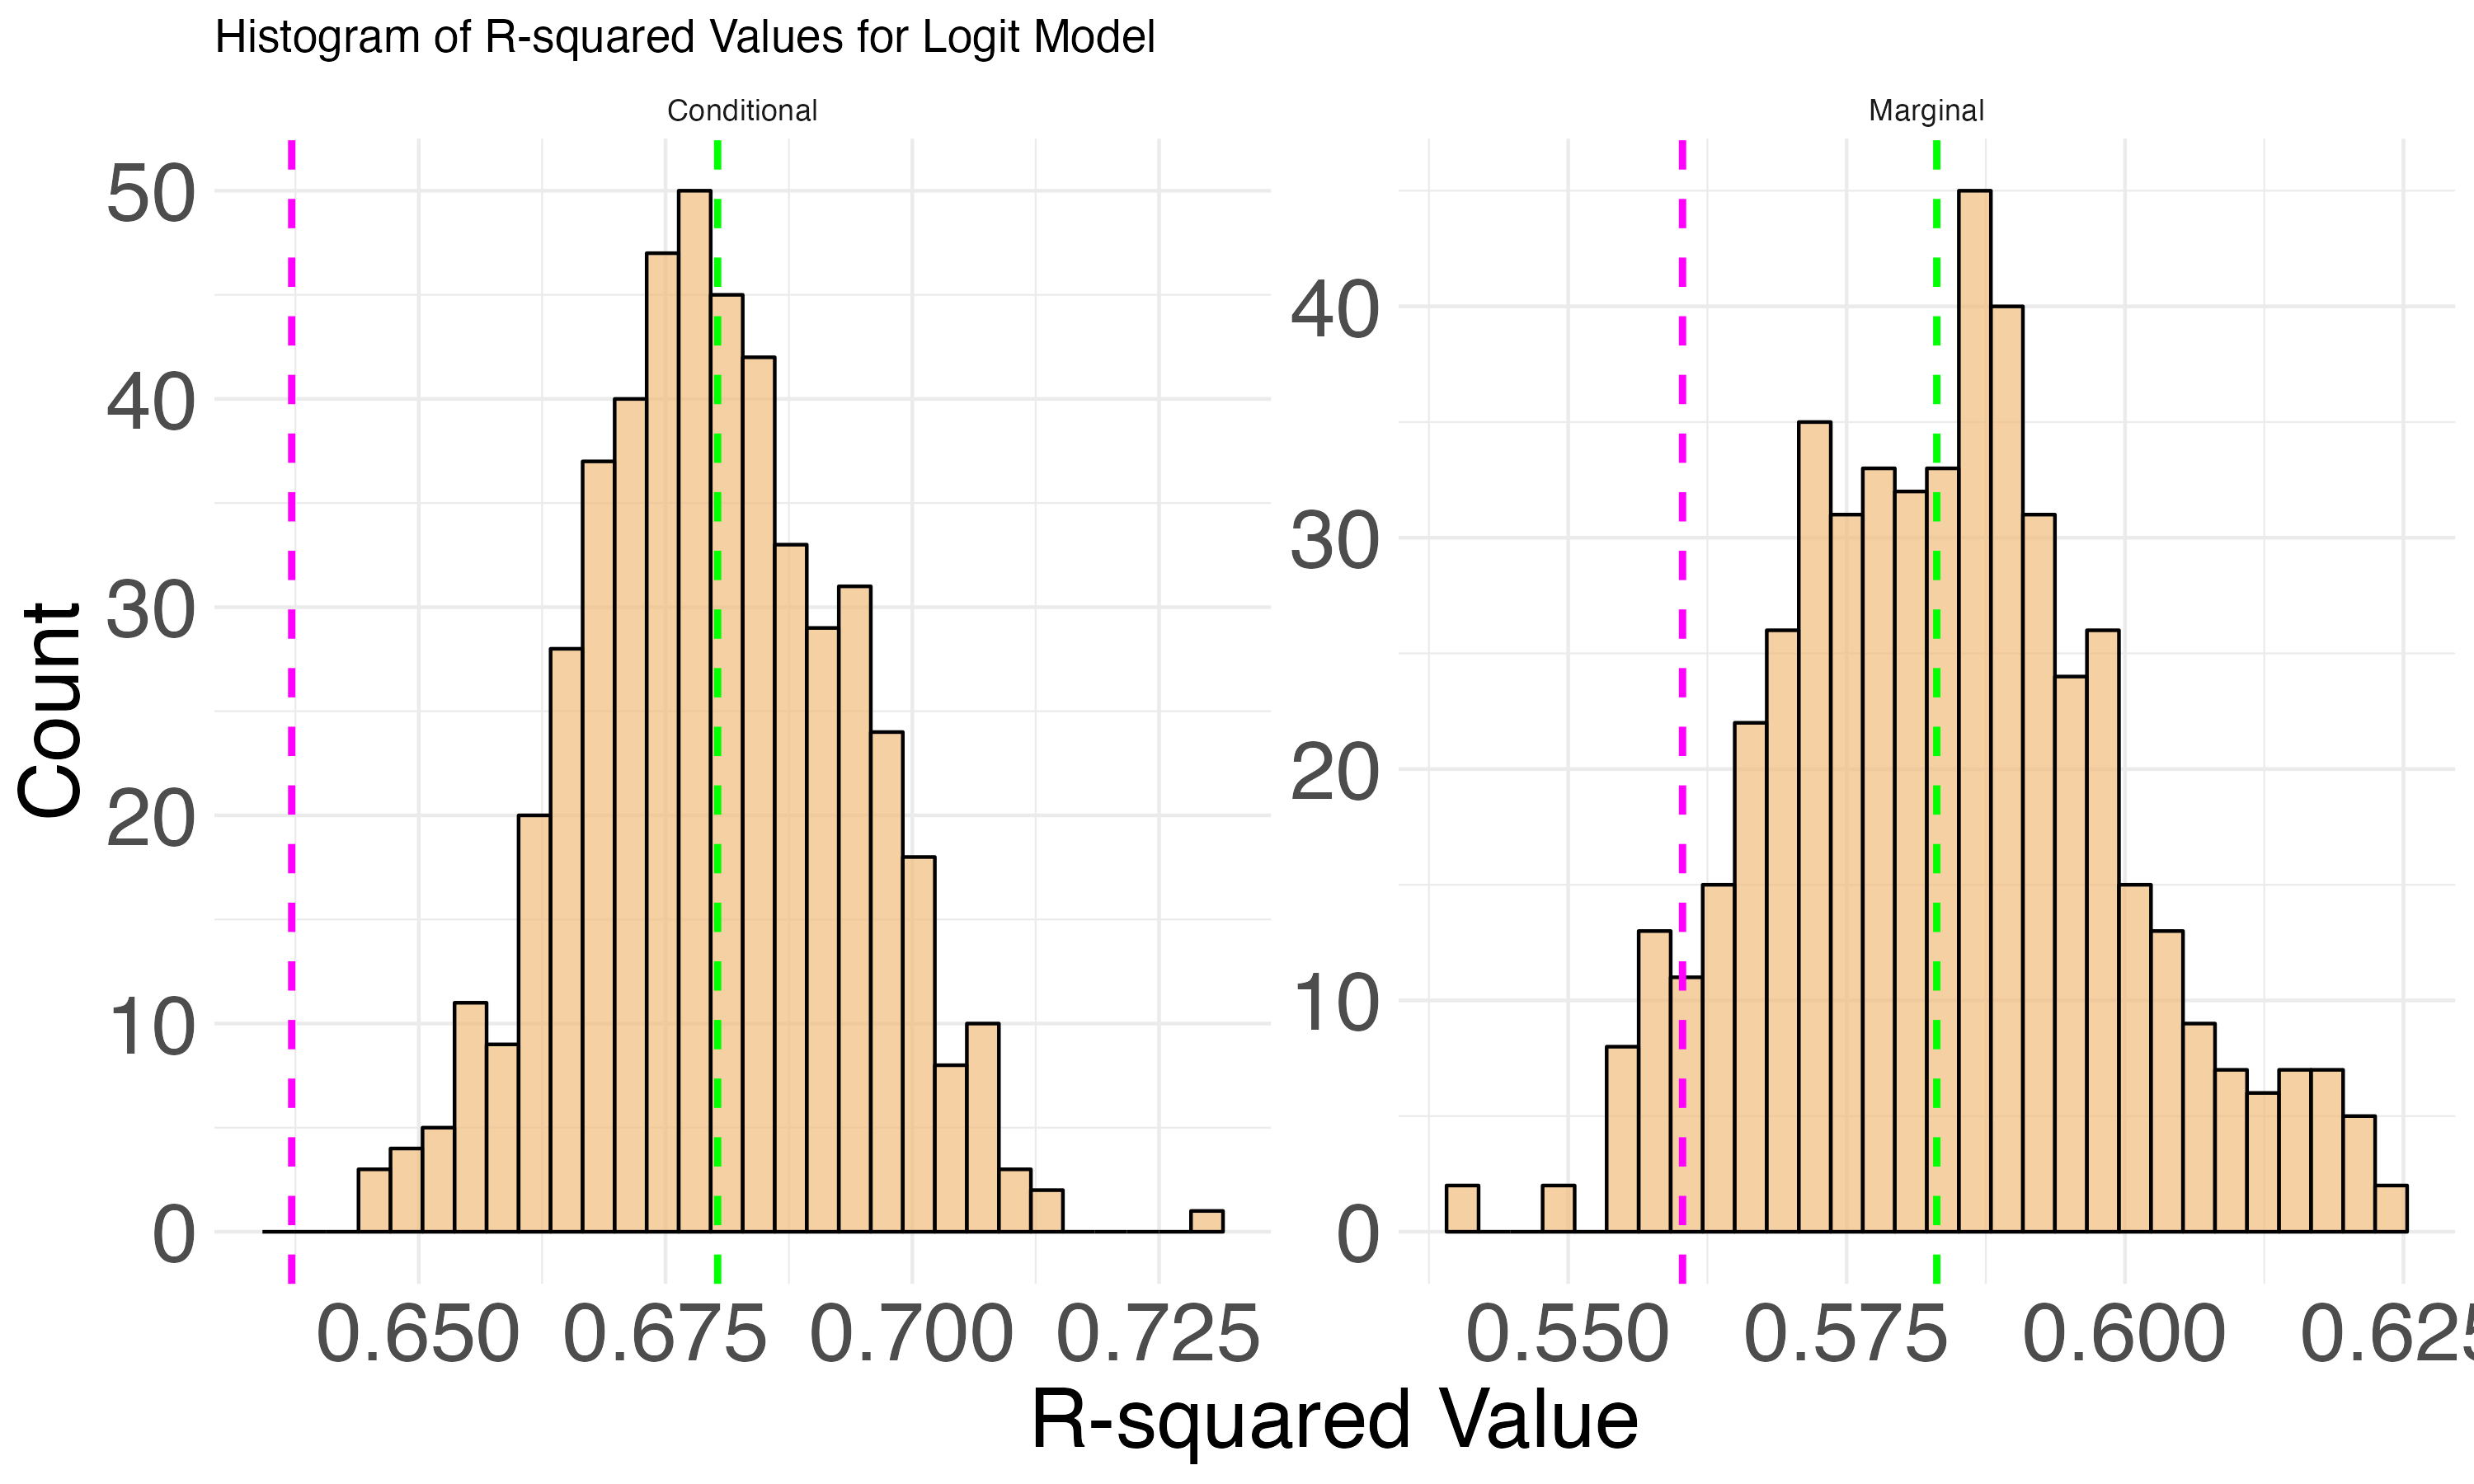
\includegraphics[width=1\linewidth]{Figures/Simulation study/R2_logit.png}
%   \caption{Conditional and marginal $R^2$ for poisson GLMM. The magenta line is Stoffel, green line is expected importance}
%     \label{fig:relimp_poisson_R2}
% \end{figure}


\section{Comparison with \texttt{rptR} package}
% \begin{figure}[H]
%     \centering
%       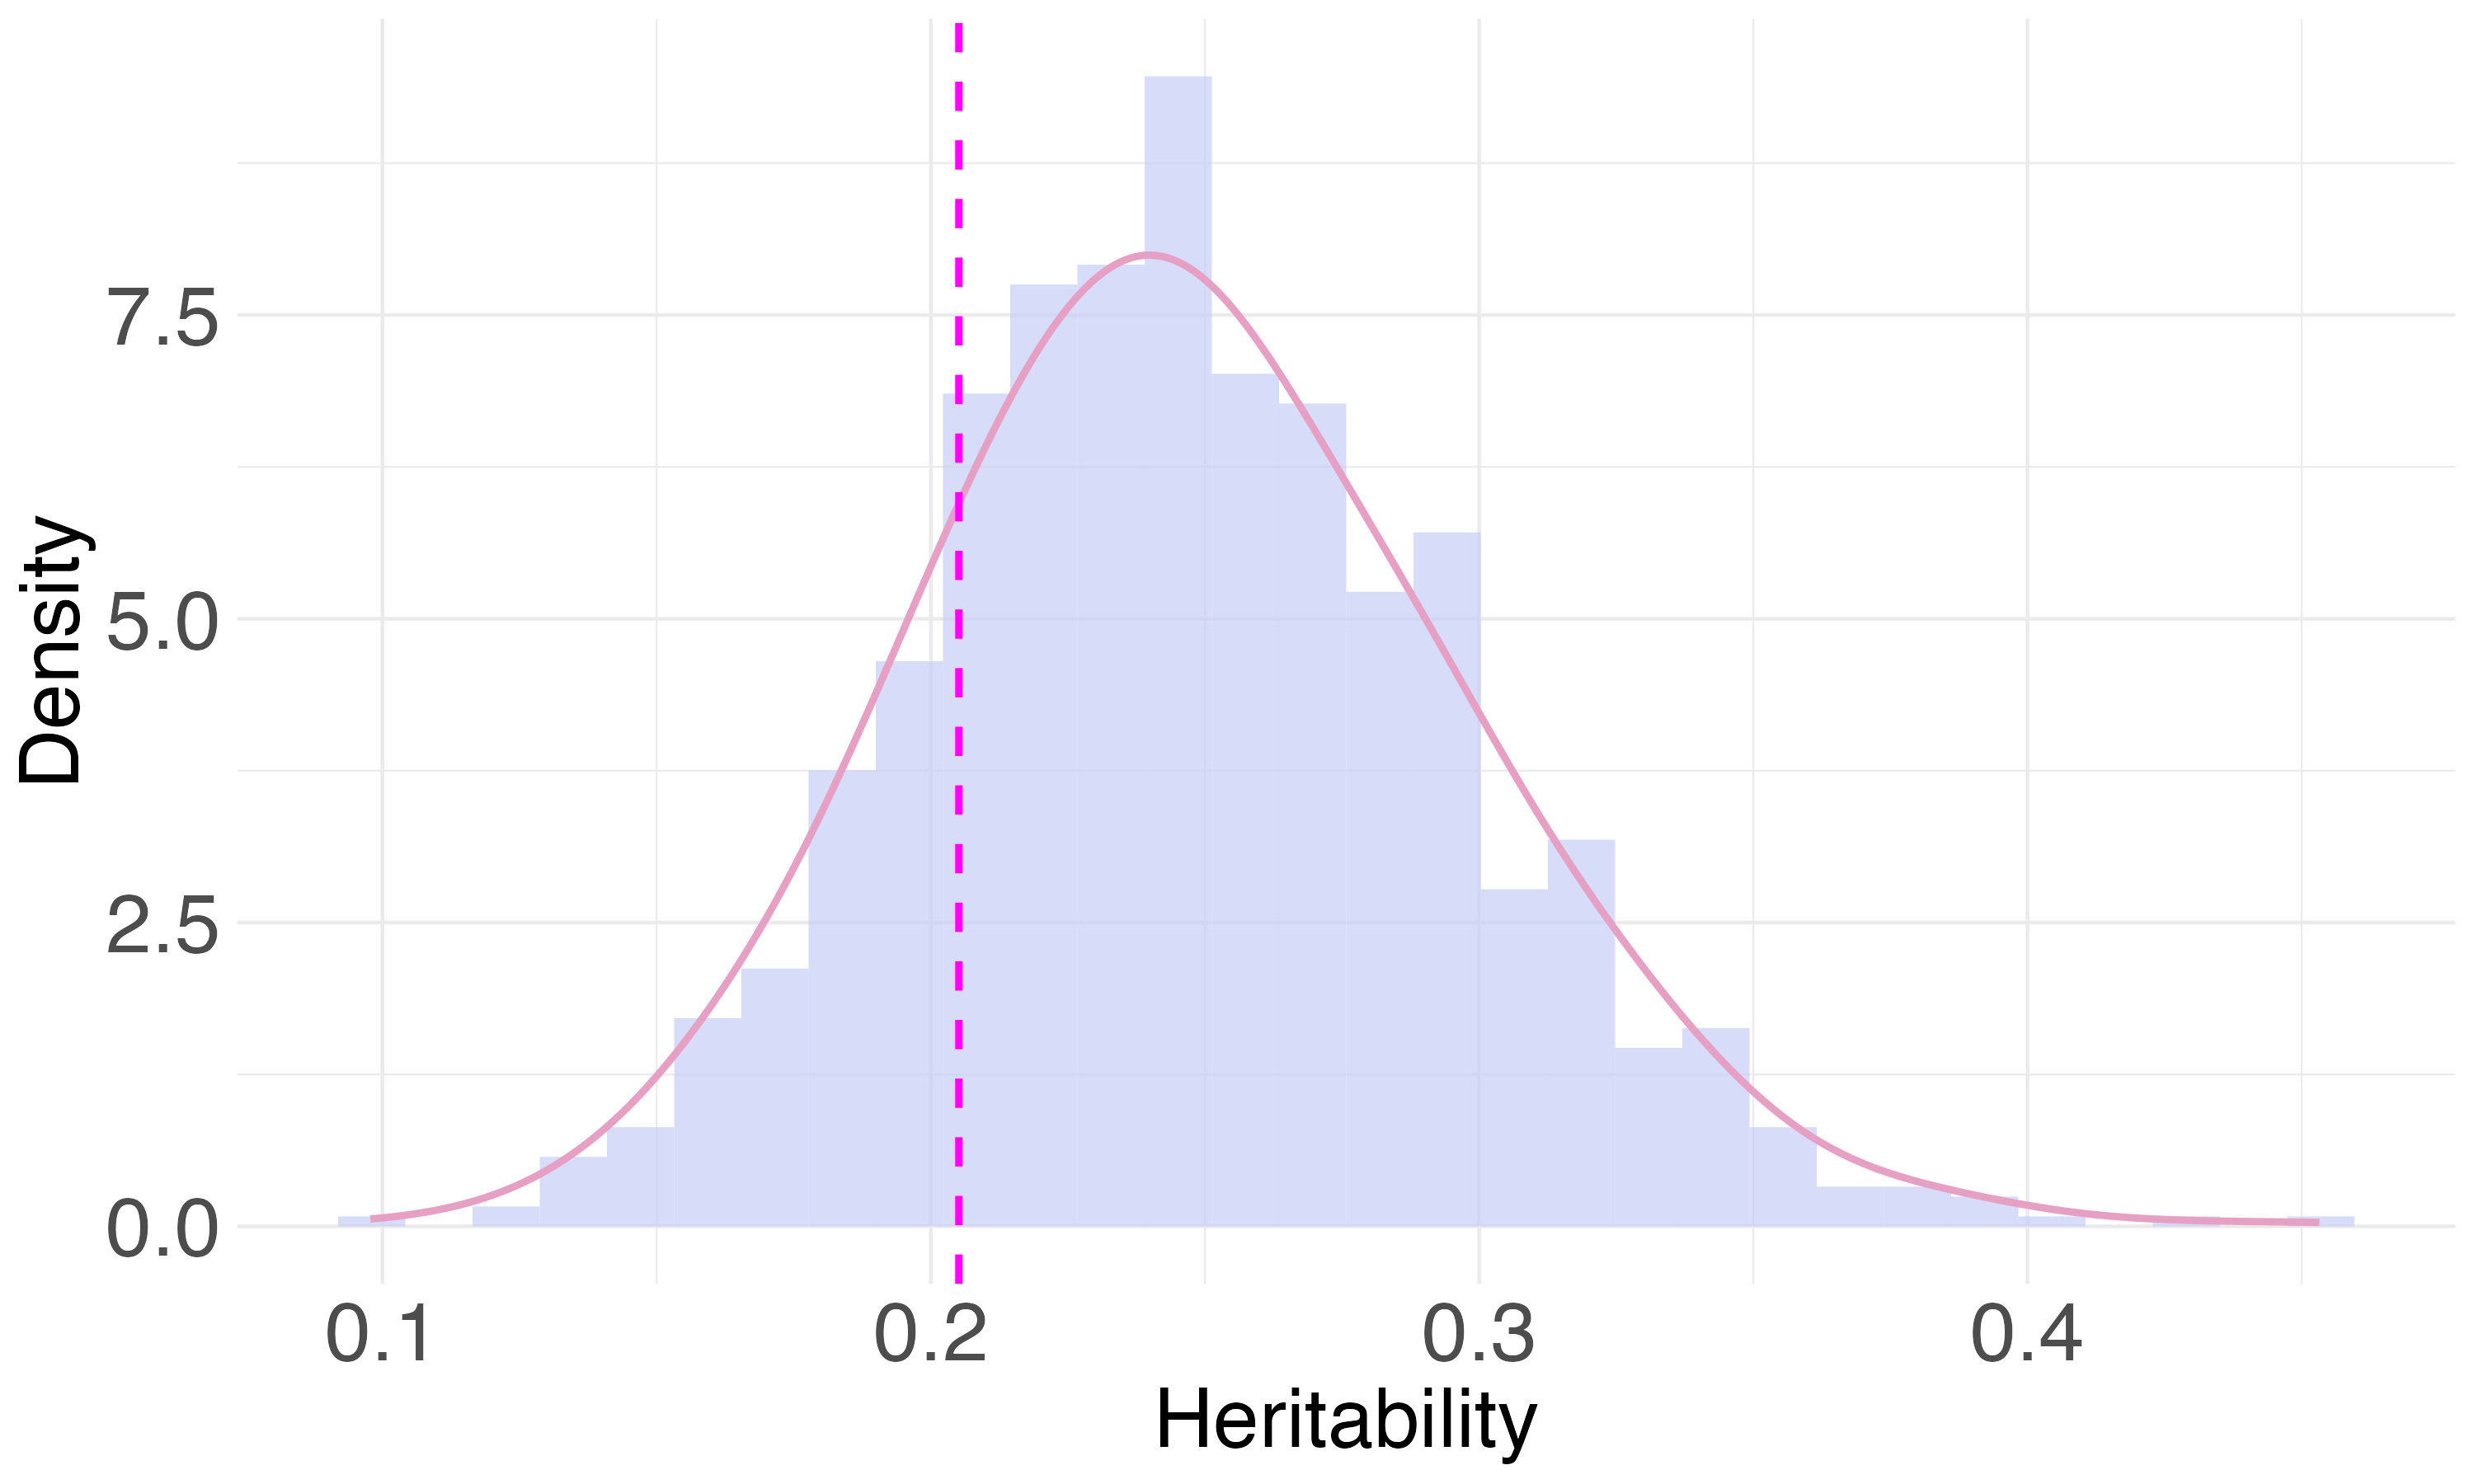
\includegraphics[width=0.7\linewidth]{Figures/Stoffel Comparison/Heritability_colour_binomial.png}
%       \caption{Heritability of colour of male beetles from Stoffel}
%       \label{fig:heritability_colour_binomial}
%   \end{figure}
%   \begin{figure}[H]\ContinuedFloat
%     \centering
%     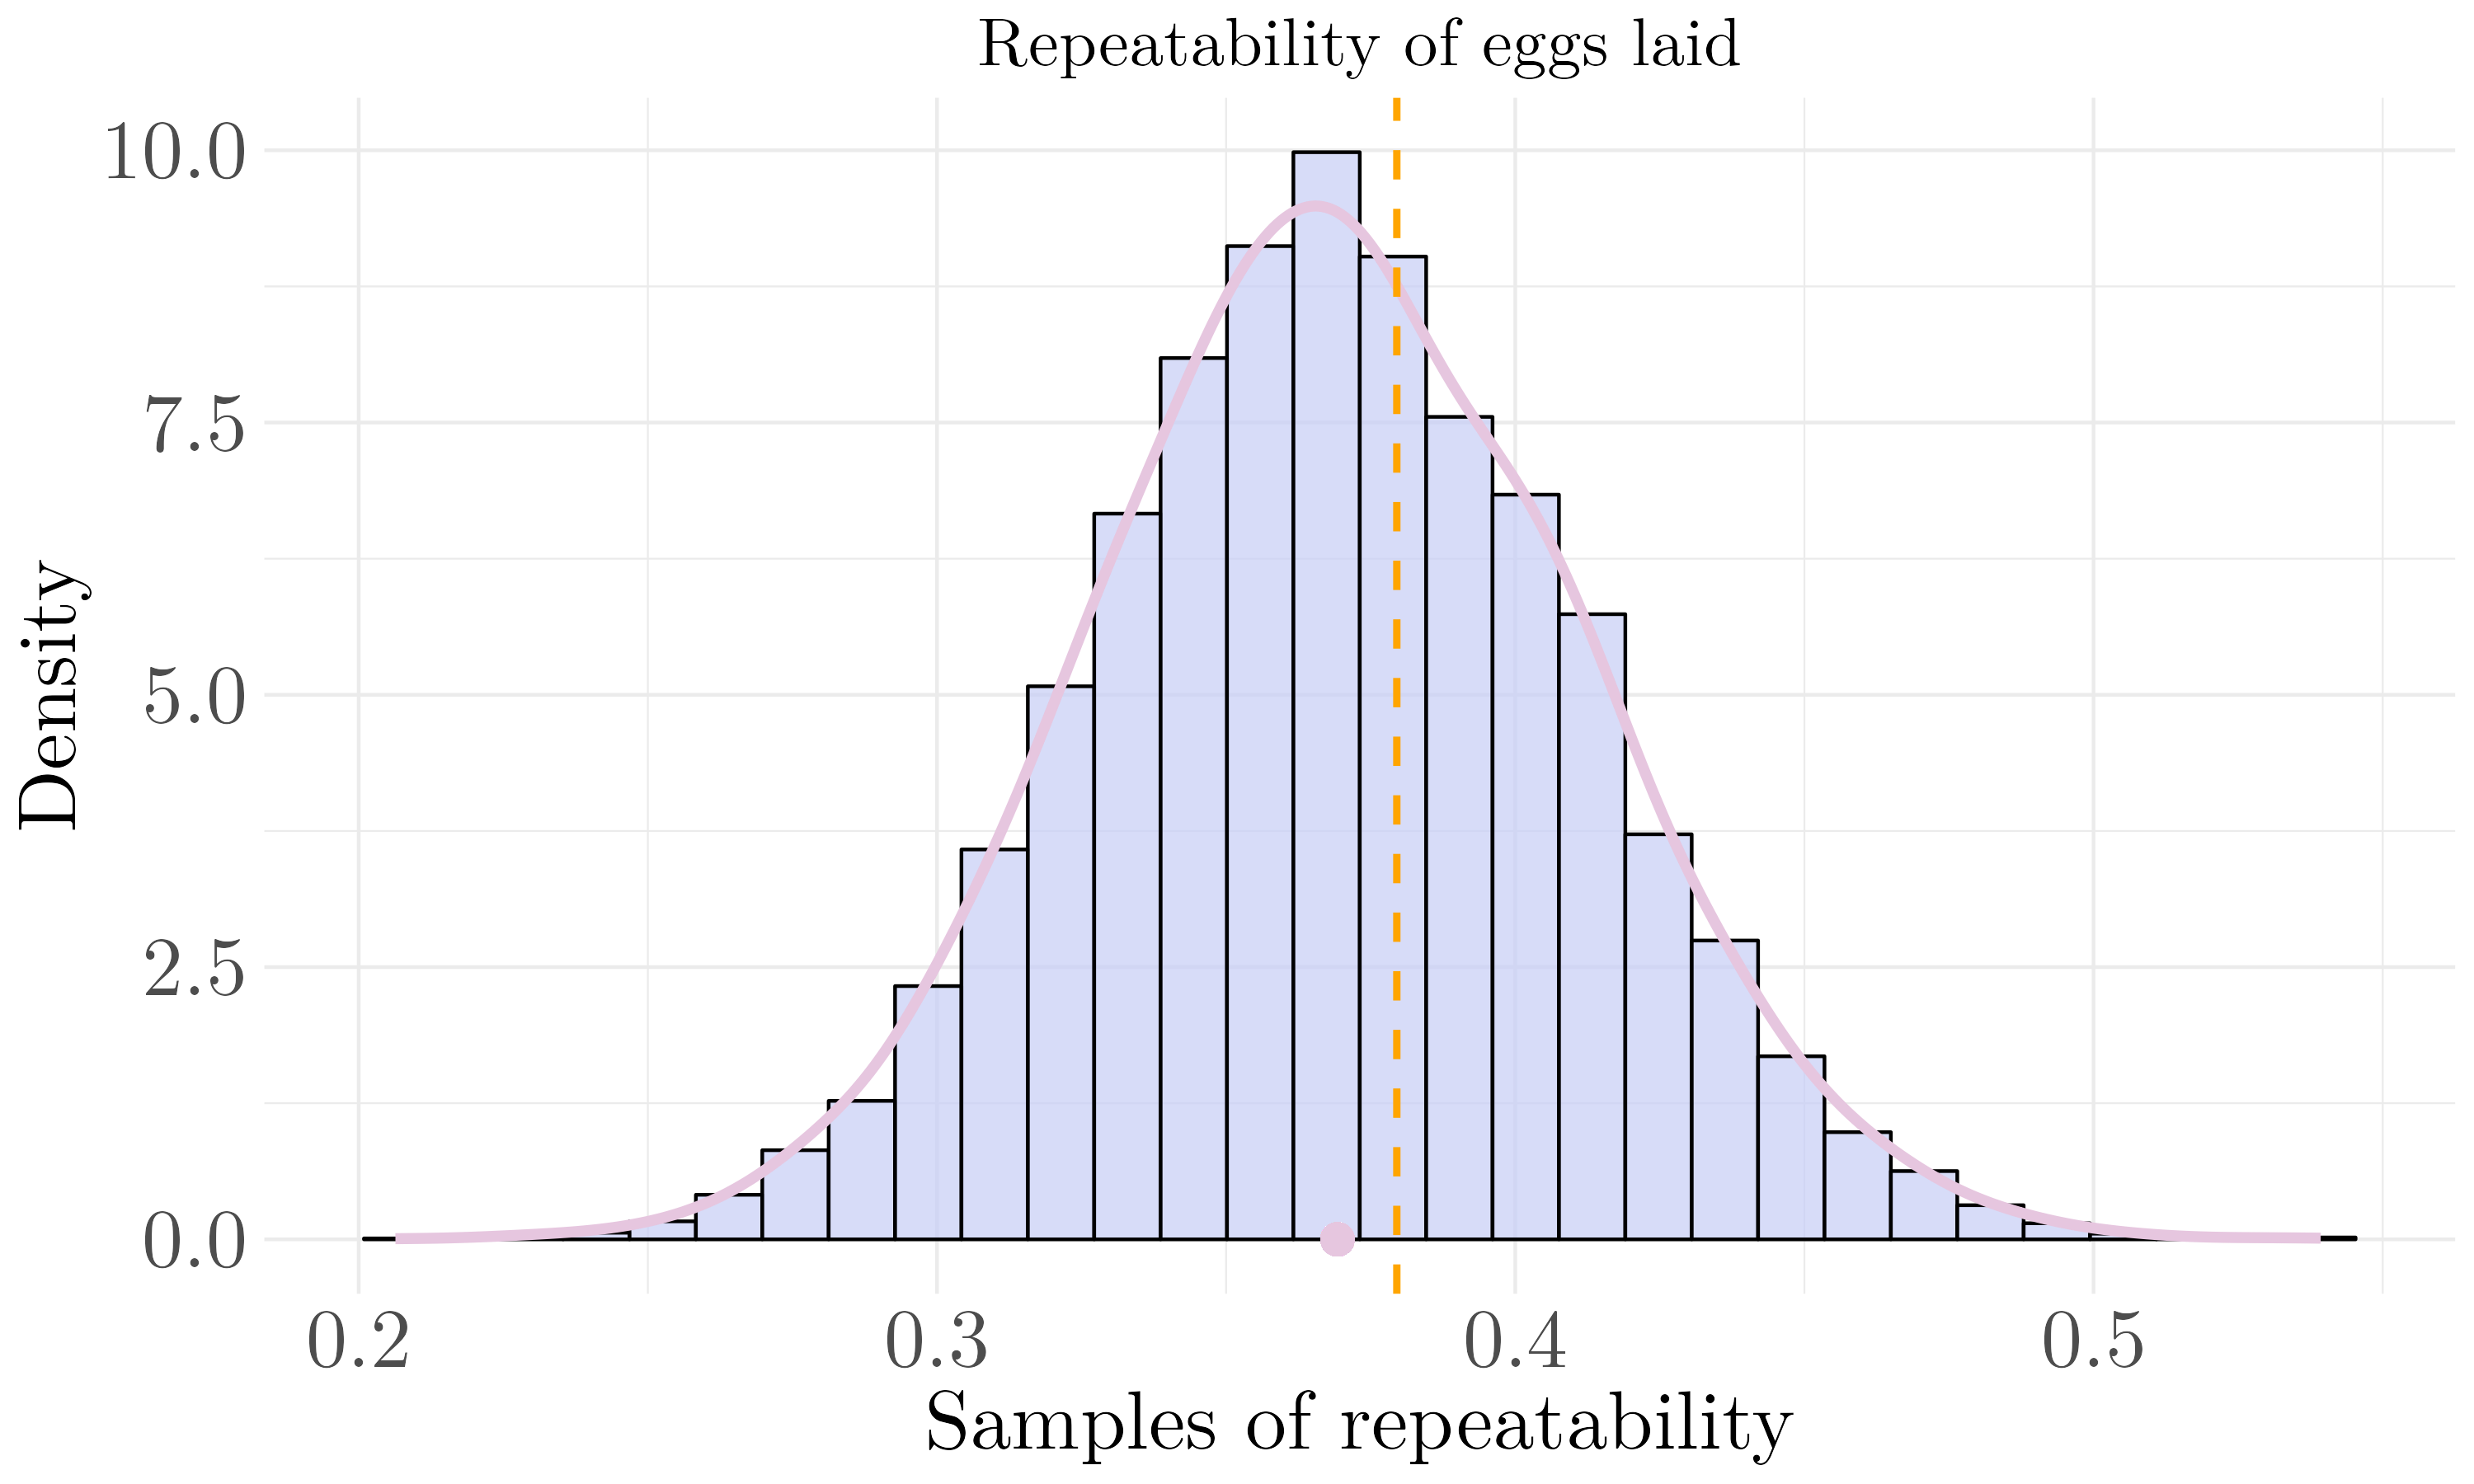
\includegraphics[width=0.7\linewidth]{Figures/Stoffel Comparison/Heritability_egg_poisson.png}
%     \caption{Heritability of eggs laid by female beetles from Stoffel}
%       \label{fig:heritability_egg_poisson}
%   \end{figure}
To further assess our method, a comparison to the vignette for the \texttt{rptR} was made. No expected results were available, and so we can only compare our method to the results made by the authors of the vignette. It should however be noted, that the \texttt{rptR} package returns the marginal $R^2$ as the only measure of importance for the fixed effects, whereas our method directly decomposes this value and assigns a share to each fixed effect. To obtain uncertainty estimates in the likelihood framework, Stoffel, Nakagawa and Schielzeth have built in bootstrap functionality. This is used in our comparison, to evaluate computational complexity and confidence intervals.
\\
\\
The heritability of the color of male beetles is modelled by a binomial GLMM with binary outcome and logit-link. We use the same formulation as in the model \texttt{rep11} from the vignette \citep{Stoffel2017rptR}, with the parameter \texttt{adjusted=FALSE}. We see that the sampled posterior distribution of heritability \Cref{fig:heritability_colour_binomial} from the Bayesian Variable Importance method is centered around a mean of $0.1922$, which is very similar to the estimate by Stoffel which is $0.1958$. The obtained distribution appears unimodal, with the mode and mean aligning closely. Perhaps a slightly longer tail on the right side can be observed. From $10^3$ bootstrap samples, the \texttt{rptR} estimates a $95\%$ confidence interval of $[0.051, 0.338]$, which is a bit larger than our estimated $95$th percentile of $[0.114, 0.279]$. In terms of computation time, the Bayesian Variable Importance method used $6$ seconds to obtain the model fit and $10^4$ samples, whereas the \texttt{rptR} package used $66$ seconds to obtain the model fit and the same number of bootstrap samples.
\begin{figure}[H]
  \centering
  % First row
  \subfloat{
    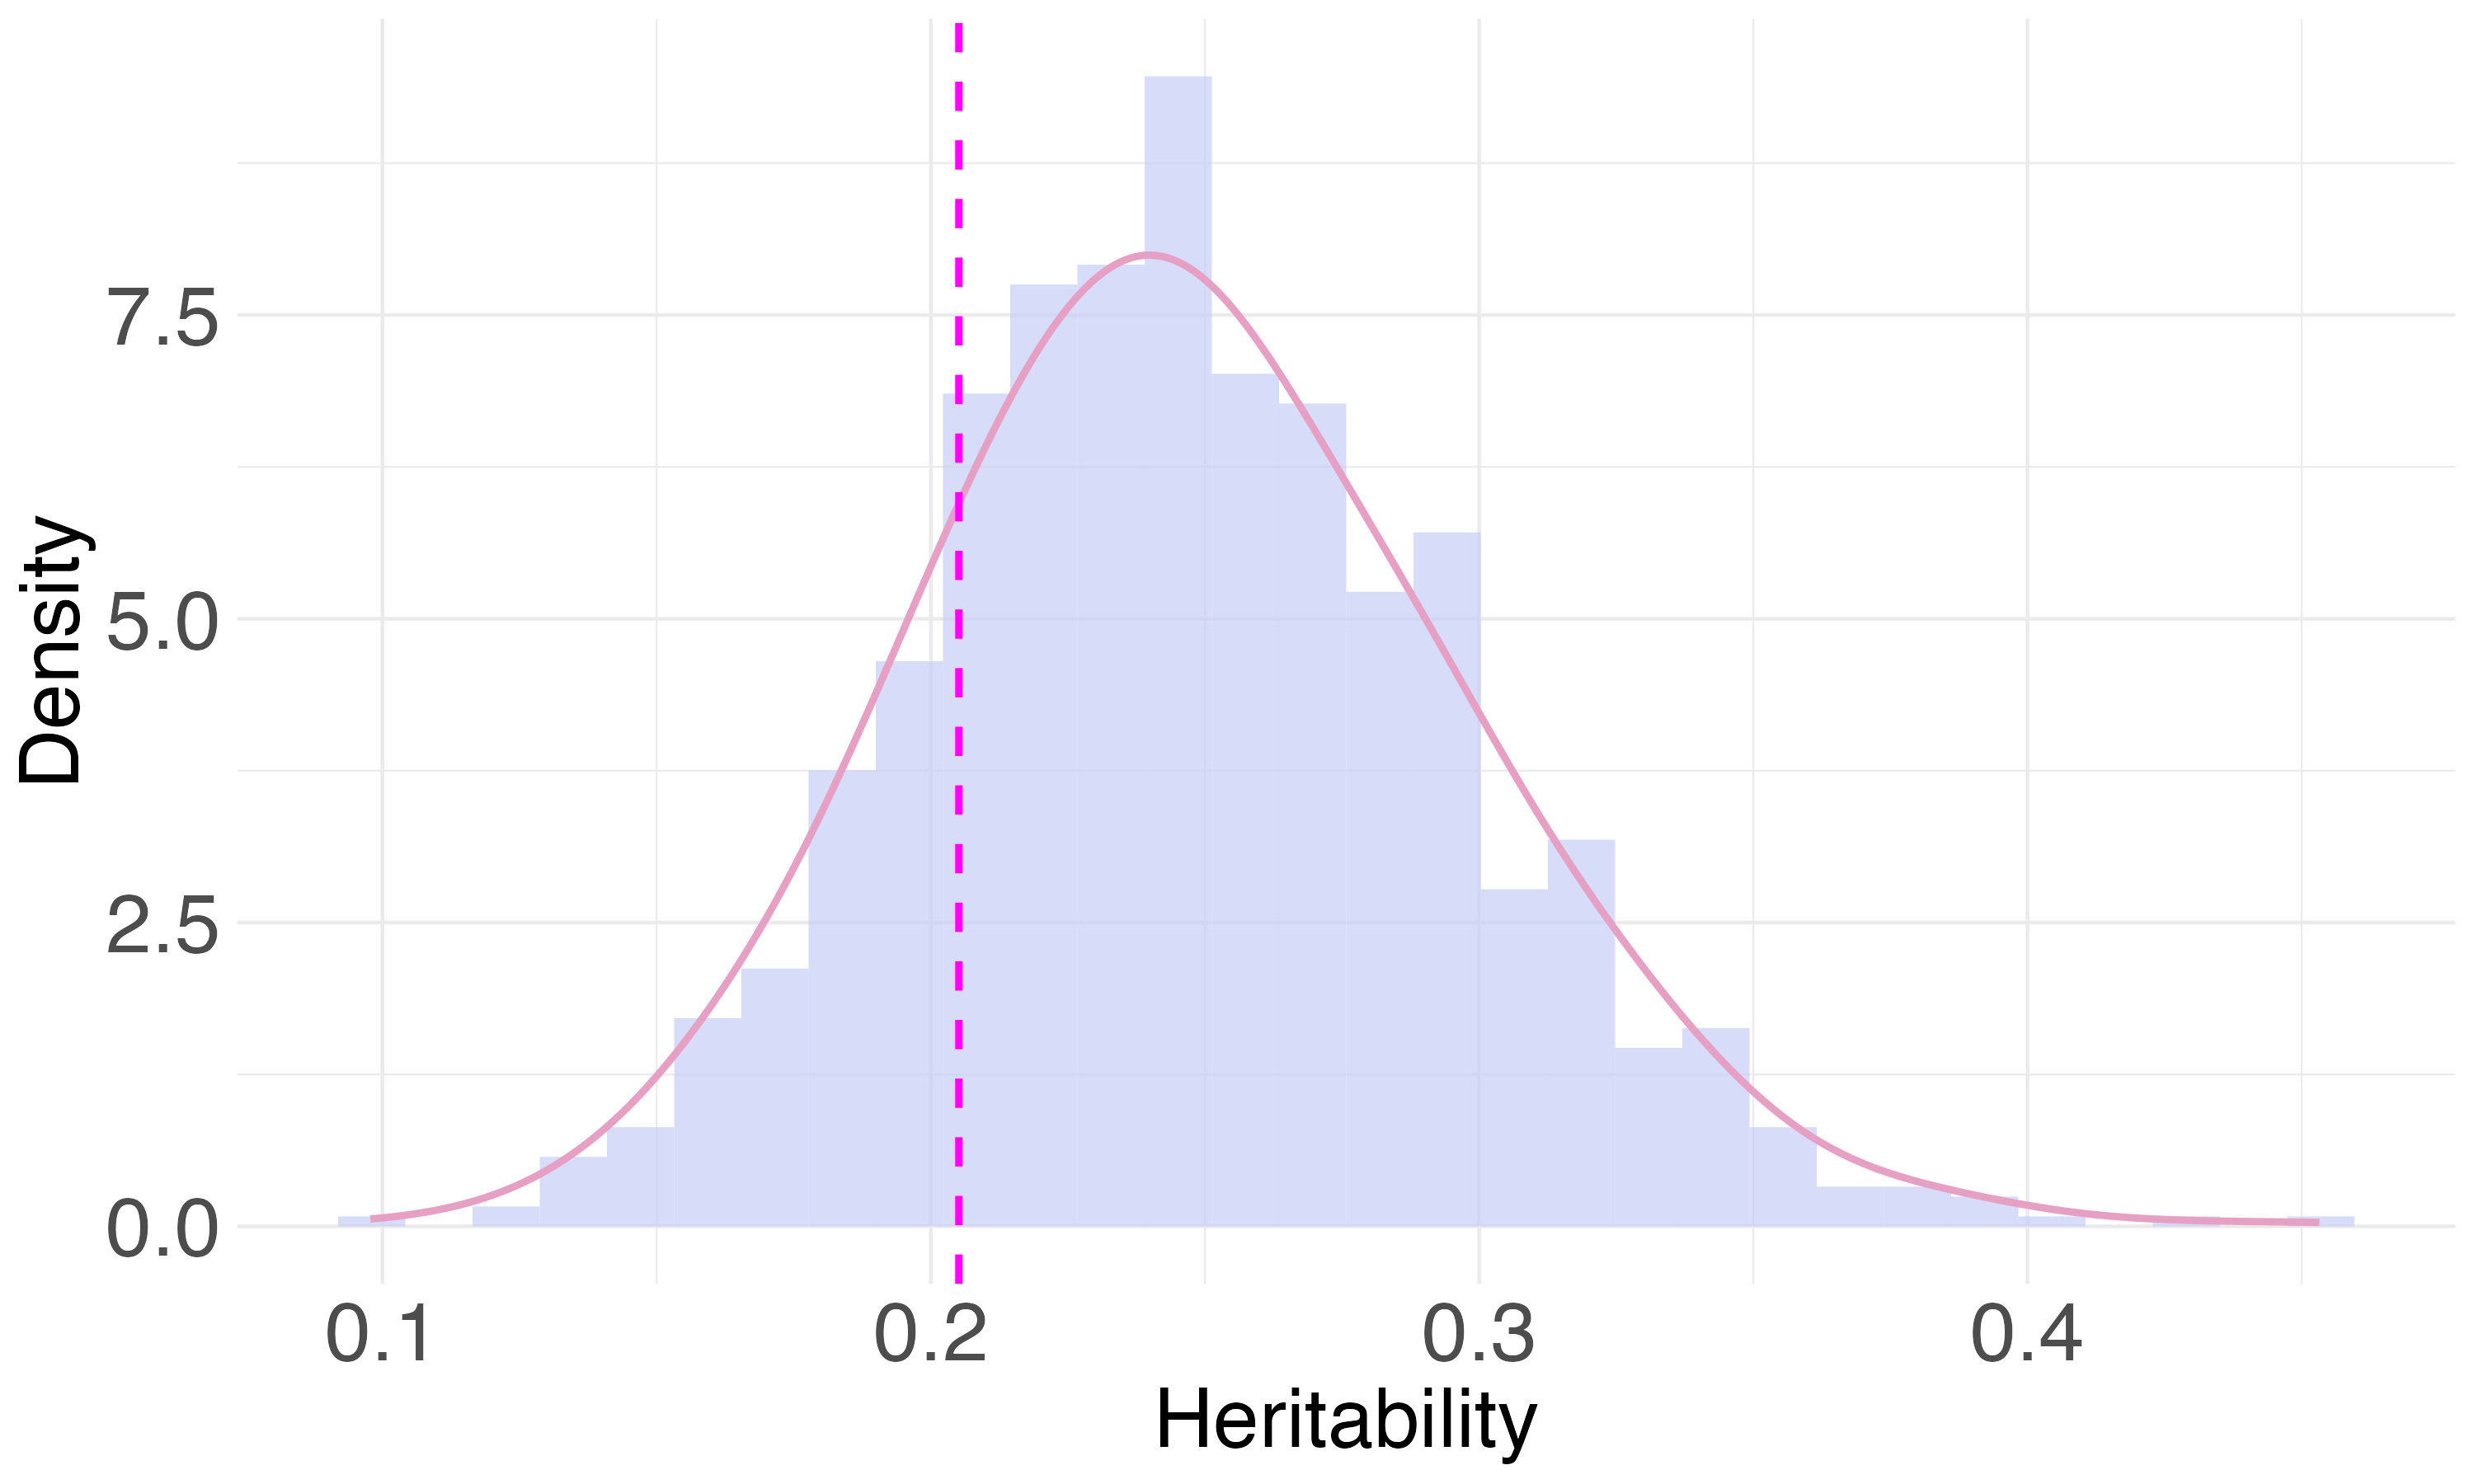
\includegraphics[width=1\linewidth]{Figures/Stoffel Comparison/Heritability_colour_binomial.png}
    \label{fig:heritability_colour_binomial}
  }
  \caption{Histogram with heritability values for the color of male beetles from the BVI method, with the estimate from the \texttt{rptR} package marked as a dashed line with orange color.}
\end{figure}
% We see that the approximated distribution from the BVI method is centered a bit to the right of the point estimate from \texttt{rptR}. The stochasticity of the BVI method makes it so that the distributions return will vary based on what seed was made to generate the results. Therefore, we expect to see a difference between the centering of the distribution and point estimates. 
\noindent To estimate the heritability of the number of eggs laid by female beetles, we use a Poisson GLMM with log-link. The model used in our method corresponds to \texttt{rep9}, but as is described in the vignette after fitting \texttt{rep9}, we set the option \texttt{expect="latent"} so that the method calculates the distributional variance as in \Cref{table:1}. This corresponds to the recommendations of \citet{nakagawa2017} as previously mentioned. Also this model is estimated from the \texttt{rptR} package with \texttt{adjusted=FALSE}. From the plotted samples of posterior heritability of eggs laid (\Cref{fig:heritability_eggs_poisson}), we see a very similar distribution as that of the binomial color model. The distribution is symmetric and centered around a mean of $0.3587$. Further, the estimate from the \texttt{rptR} model is $0.3795$ with a confidence interval of $[0.131, 0.542]$, compared to our $95$th percentile of $[0.277, 0.442]$. The $10^3$ bootstrap samples and model fit for the \texttt{rptR} package took $2$ minutes and $13$ seconds, whereas the BVI method used $8$ seconds to obtain the model fit and $10^4$ samples.
% \begin{figure}[H]
%   \centering
%   \begin{subfloat}{0.49\linewidth}
%       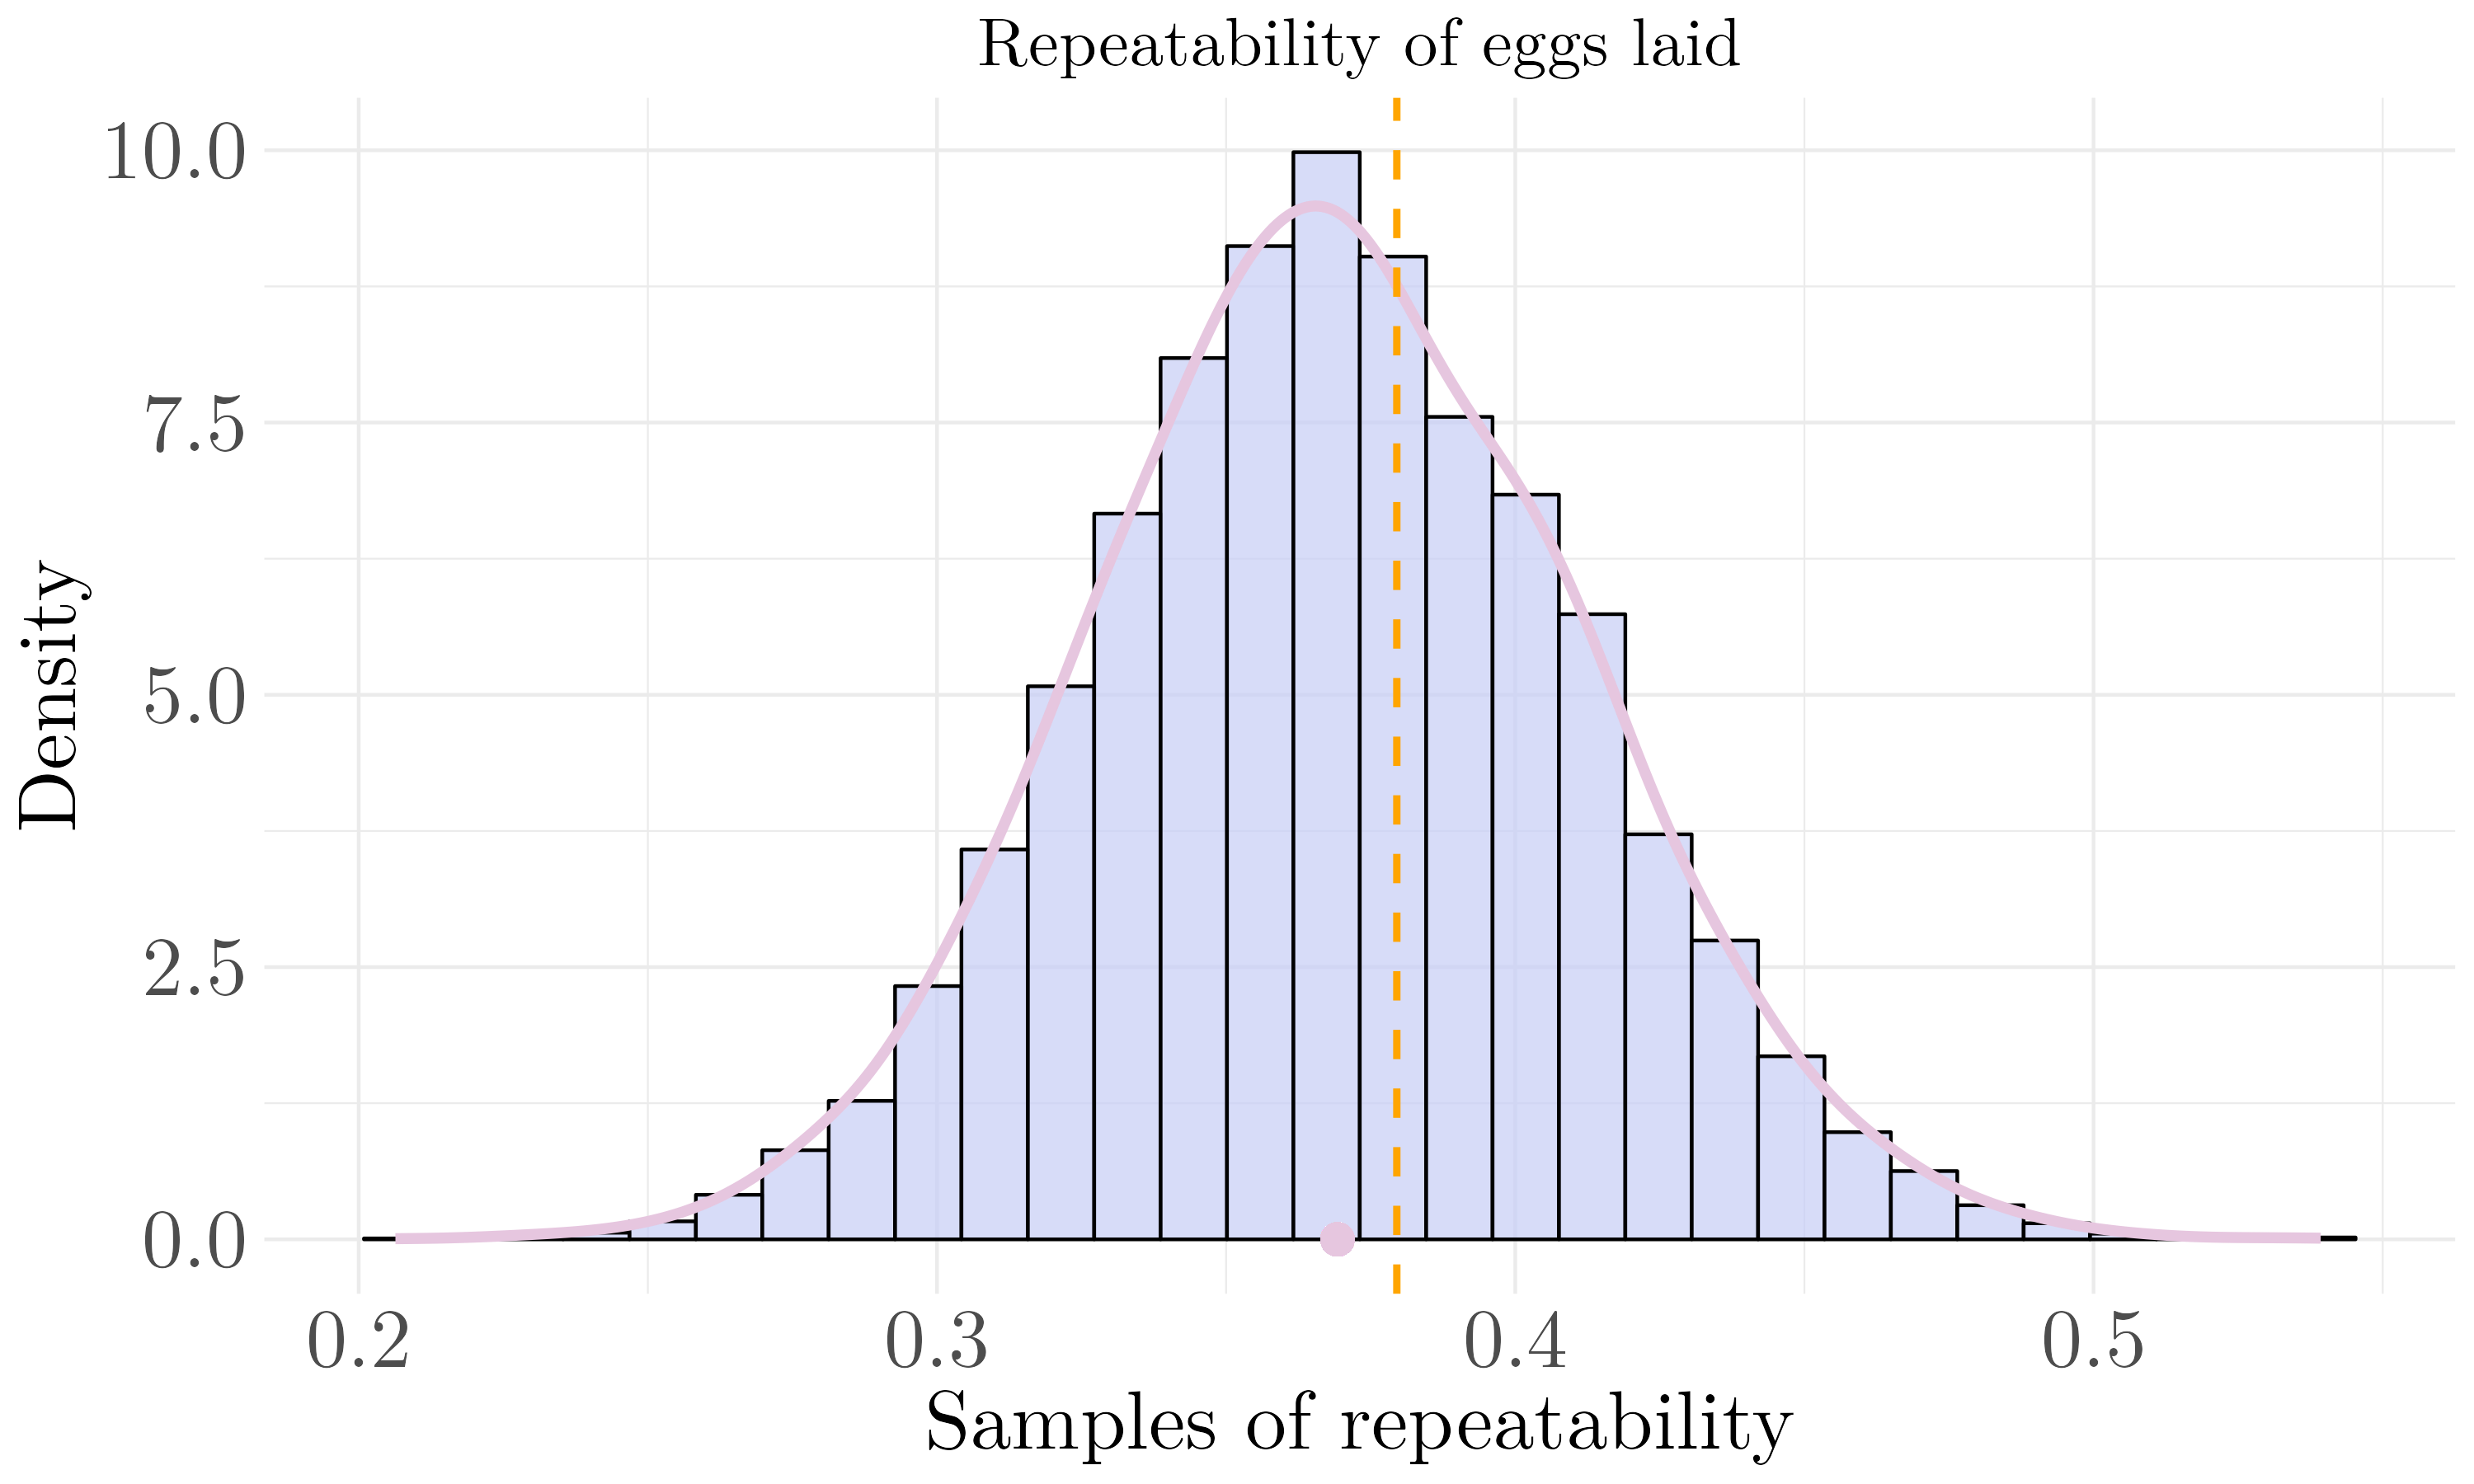
\includegraphics[width=\linewidth]{Figures/Stoffel Comparison/Heritability_egg_poisson.png}
%       \caption{Heritability of eggs laid by female beetles from BVI}
%       \label{fig:heritability_egg_poisson}
%   \end{subfloat}
%   \hfill
%   \begin{subfloat}{0.49\linewidth}
%       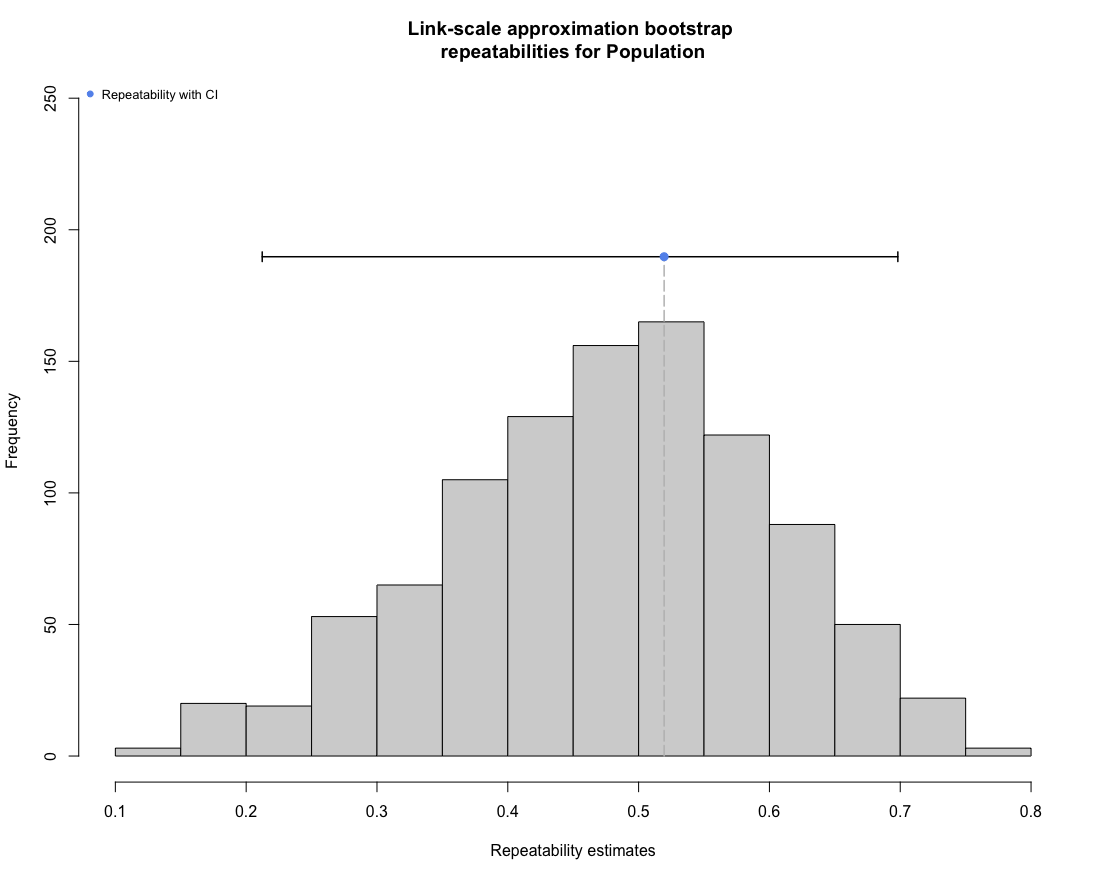
\includegraphics[width=\linewidth]{Figures/Stoffel Comparison/Heritability_egg_poisson_Stoffel.png}
%       \caption{Comparison of heritability of eggs from Stoffel}
%       \label{fig:comparison_heritability_egg}
%   \end{subfloat}
%   \caption{Heritability of eggs in female beetles and comparison}
% \end{figure}
\begin{figure}[H]
  \centering
  % First row
  \subfloat{
    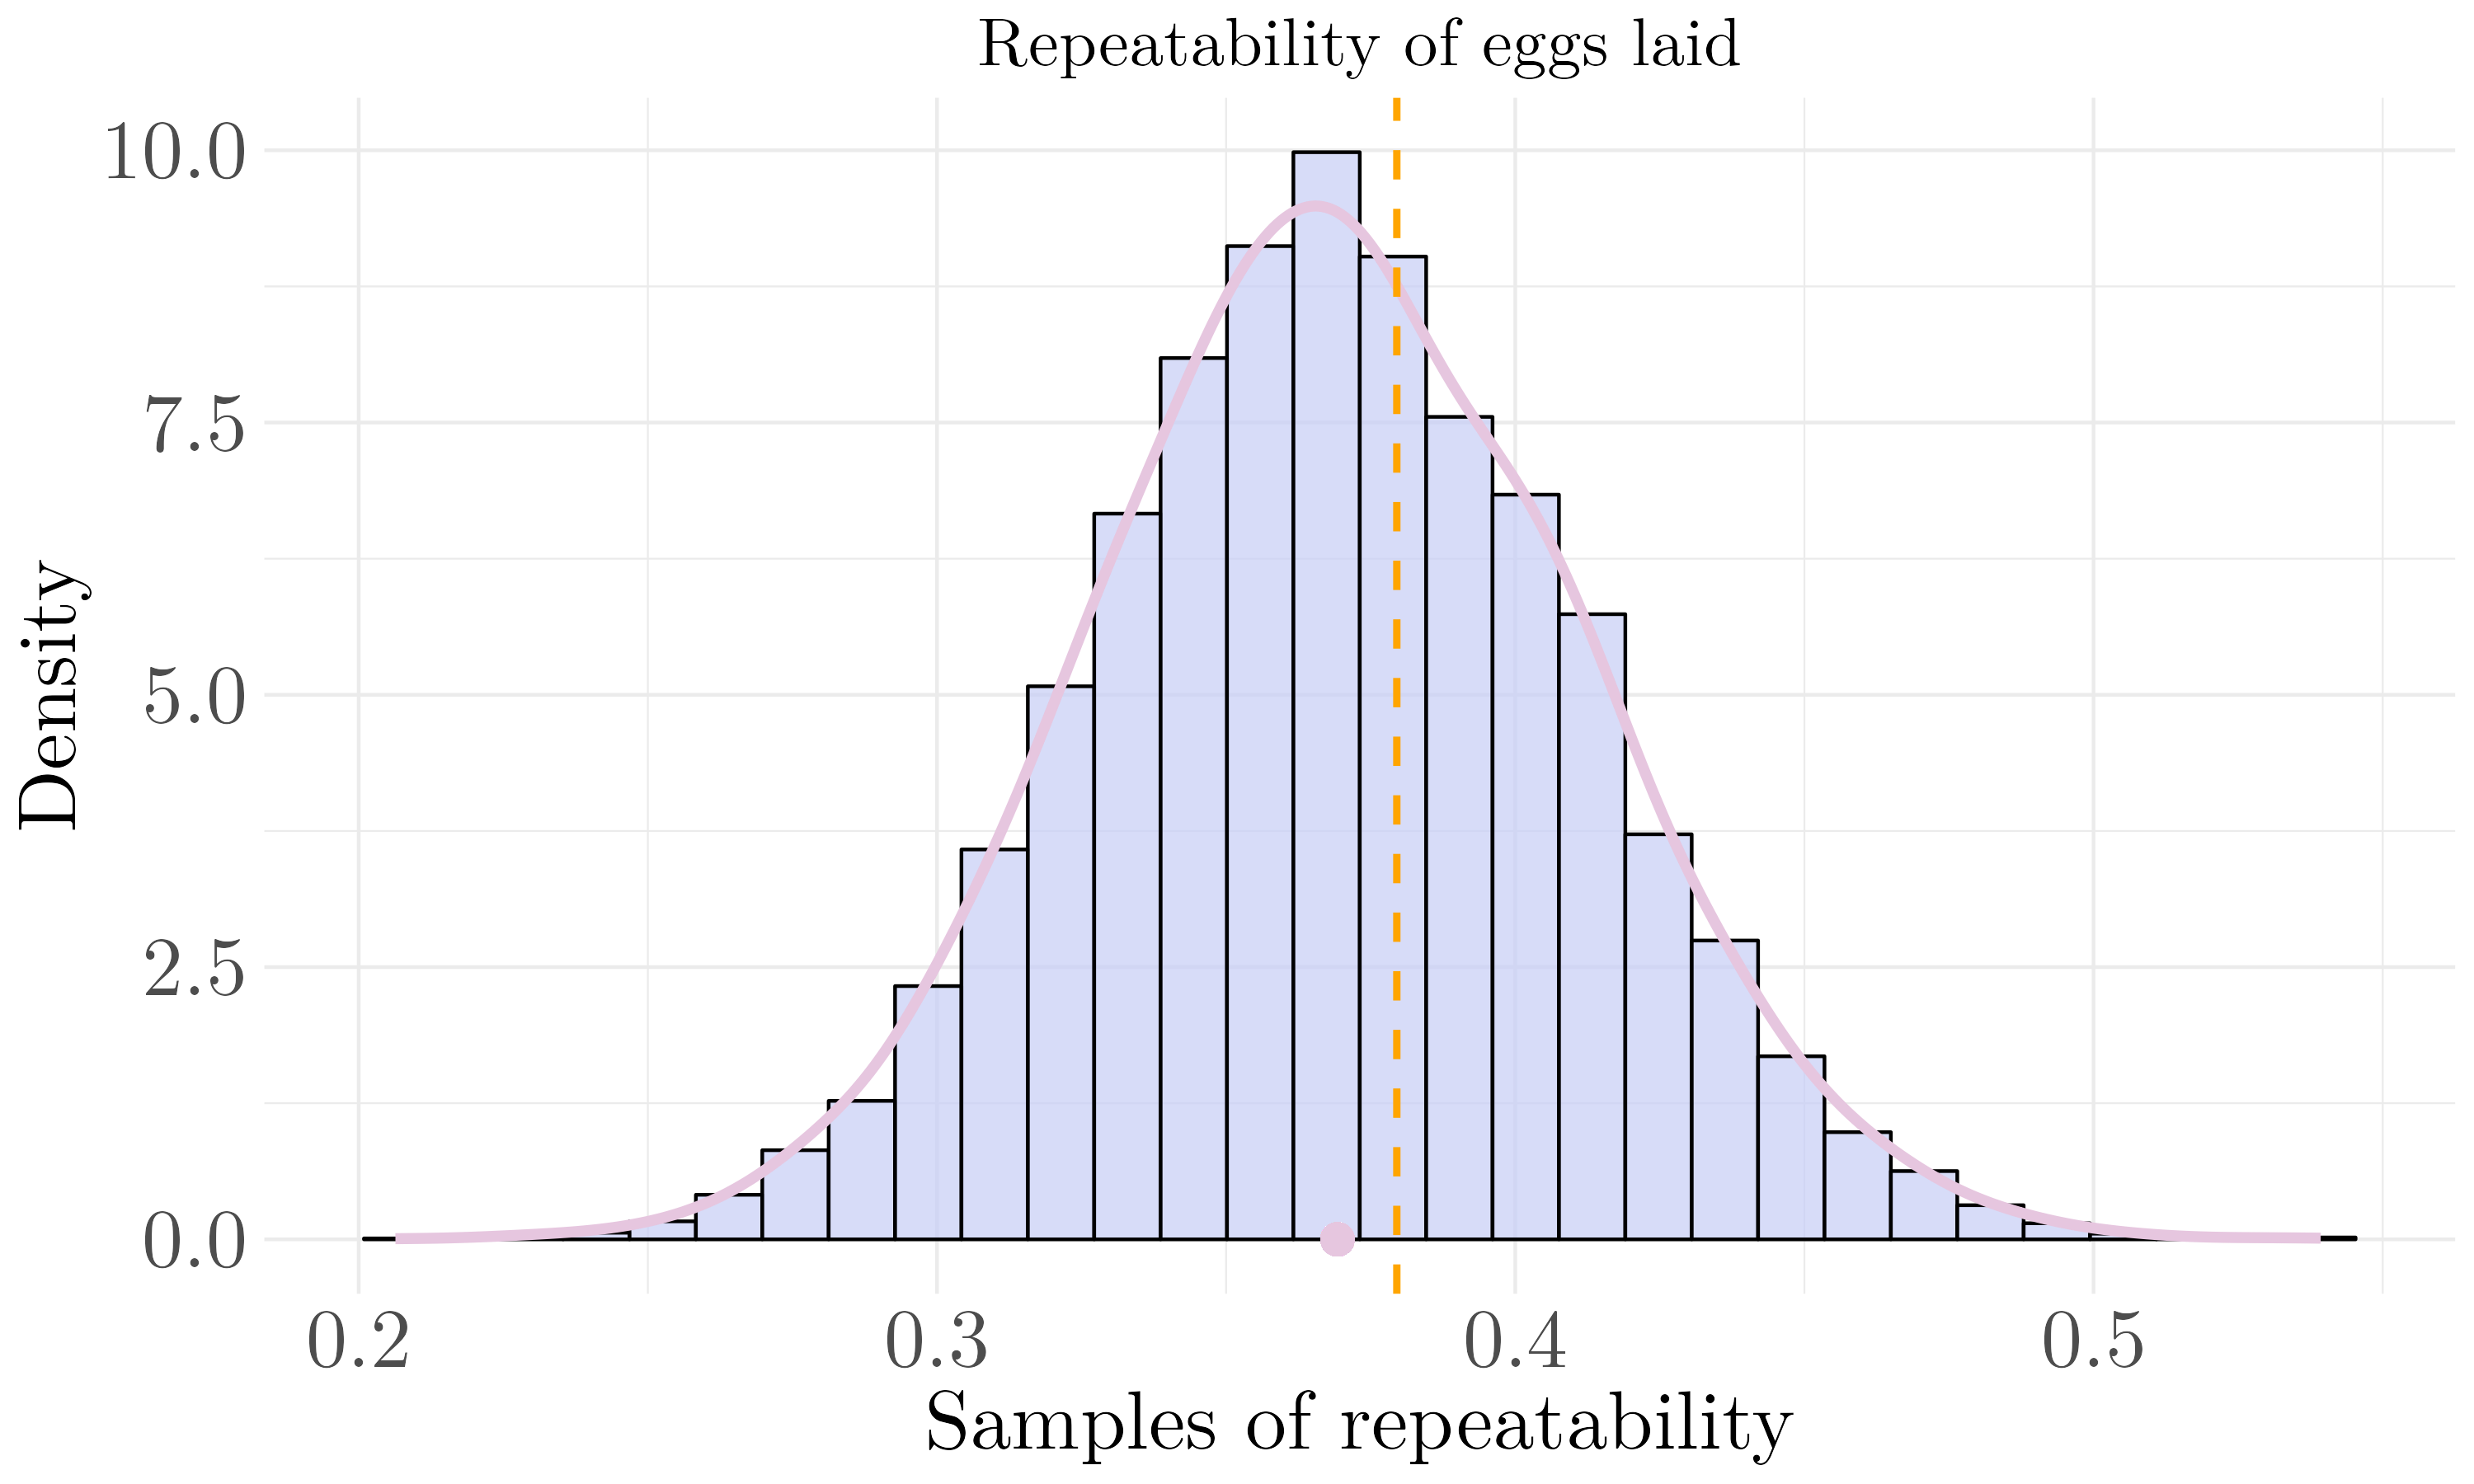
\includegraphics[width=1\linewidth]{Figures/Stoffel Comparison/Heritability_egg_poisson.png}
    \label{fig:heritability_eggs_poisson}
  }
  \caption{Histogram with heritability values for eggs laid by female beetles from BVI method, with the estimate from the \texttt{rptR} package marked as a dashed line with orange color.}
\end{figure}
\noindent It should perhaps be mentioned, that the estimates from the BVI method will vary each time a model is fit, as it is stochastic. Therefore, it could be that another fit from the BVI method might align closer with Stoffels results, but it could also be further off. 
\section{Heritability of house sparrow traits}
We now investigate the results of applying our method to the house sparrow dataset. As previously discussed (\Cref{sec:heritability}), estimating the heritability of phenotypic traits can be seen as a special case of relative variable importance and so the findings we present are directly obtained by our method. The samples of relative variable importance presented, are sampled from the variance component that captures additive genetic variance, and we use the results from \citet{Silva2017} and \citet{Muff2019Genetic} to compare with. For this case, the covariance structure of the pedigree required us to model more complex random effects than i.i.d. random intercepts, and so the \texttt{rptR} package could not be used for comparisons. In \Cref{table:summary_heritability} the mean of sampled heritability along with confidence intervals is presented, as well as the corresponding measures from the comparable studies.
\begin{table}[H]
  \centering
  \begin{tabular}{lccccccc}
  \toprule
   & \multicolumn{2}{c}{\citet{Silva2017}} & \multicolumn{2}{c}{\citet{Muff2019Genetic}} & \multicolumn{2}{c}{BVI} \\ 
   \cmidrule(lr){2-3} \cmidrule(lr){4-5} \cmidrule(lr){6-7}
   & Estimate & CI & Estimate & CI & Mean & CI \\ 
  \midrule
  $h^2_{\text{mass}}$    & 0.300 & [0.231, 0.369] & 0.288 & [0.219, 0.371] & 0.283 & [0.232, 0.344] \\
  $h^2_{\text{wing}}$    & 0.388 & [0.353, 0.461] & 0.344 & [0.294, 0.409] & 0.356 & [0.322, 0.393] \\
  $h^2_{\text{tarsus}}$  & 0.415 & [0.333, 0.497] & - & - & 0.401 & [0.330, 0.470] \\ 
  \bottomrule
  \end{tabular}
  \caption{Heritability estimates and confidence interval from \citet{Silva2017}, posterior means of additive genetic variance divided by the posterior means of total phenotypic variance in \citet{Muff2019Genetic} with corresponding confidence interval and the mean and confidence interval of the heritability samples obtained from the BVI method for the phenotypic traits; body mass, wing length and tarsus length.}
  \label{table:summary_heritability}
\end{table}
\noindent For the sampled heritability of body mass (\Cref{fig:heritability_mass}), we have a mean of $0.2838$ (\Cref{table:summary_heritability}) and a distribution that is centered around the mean. The distribution does not seem to be symmetric, and might show signs of being bimodal, with one larger peak at the mean and possibly one smaller peak to the left of the larger peak. Furthermore, the distribution exhibits a longer tail to the right and the $95$th percentile is approximately the interval $[0.2324, 0.3430]$. To fit the model and obtain the samples, the method took about $73$ seconds.
\begin{figure}[H]
  \centering
    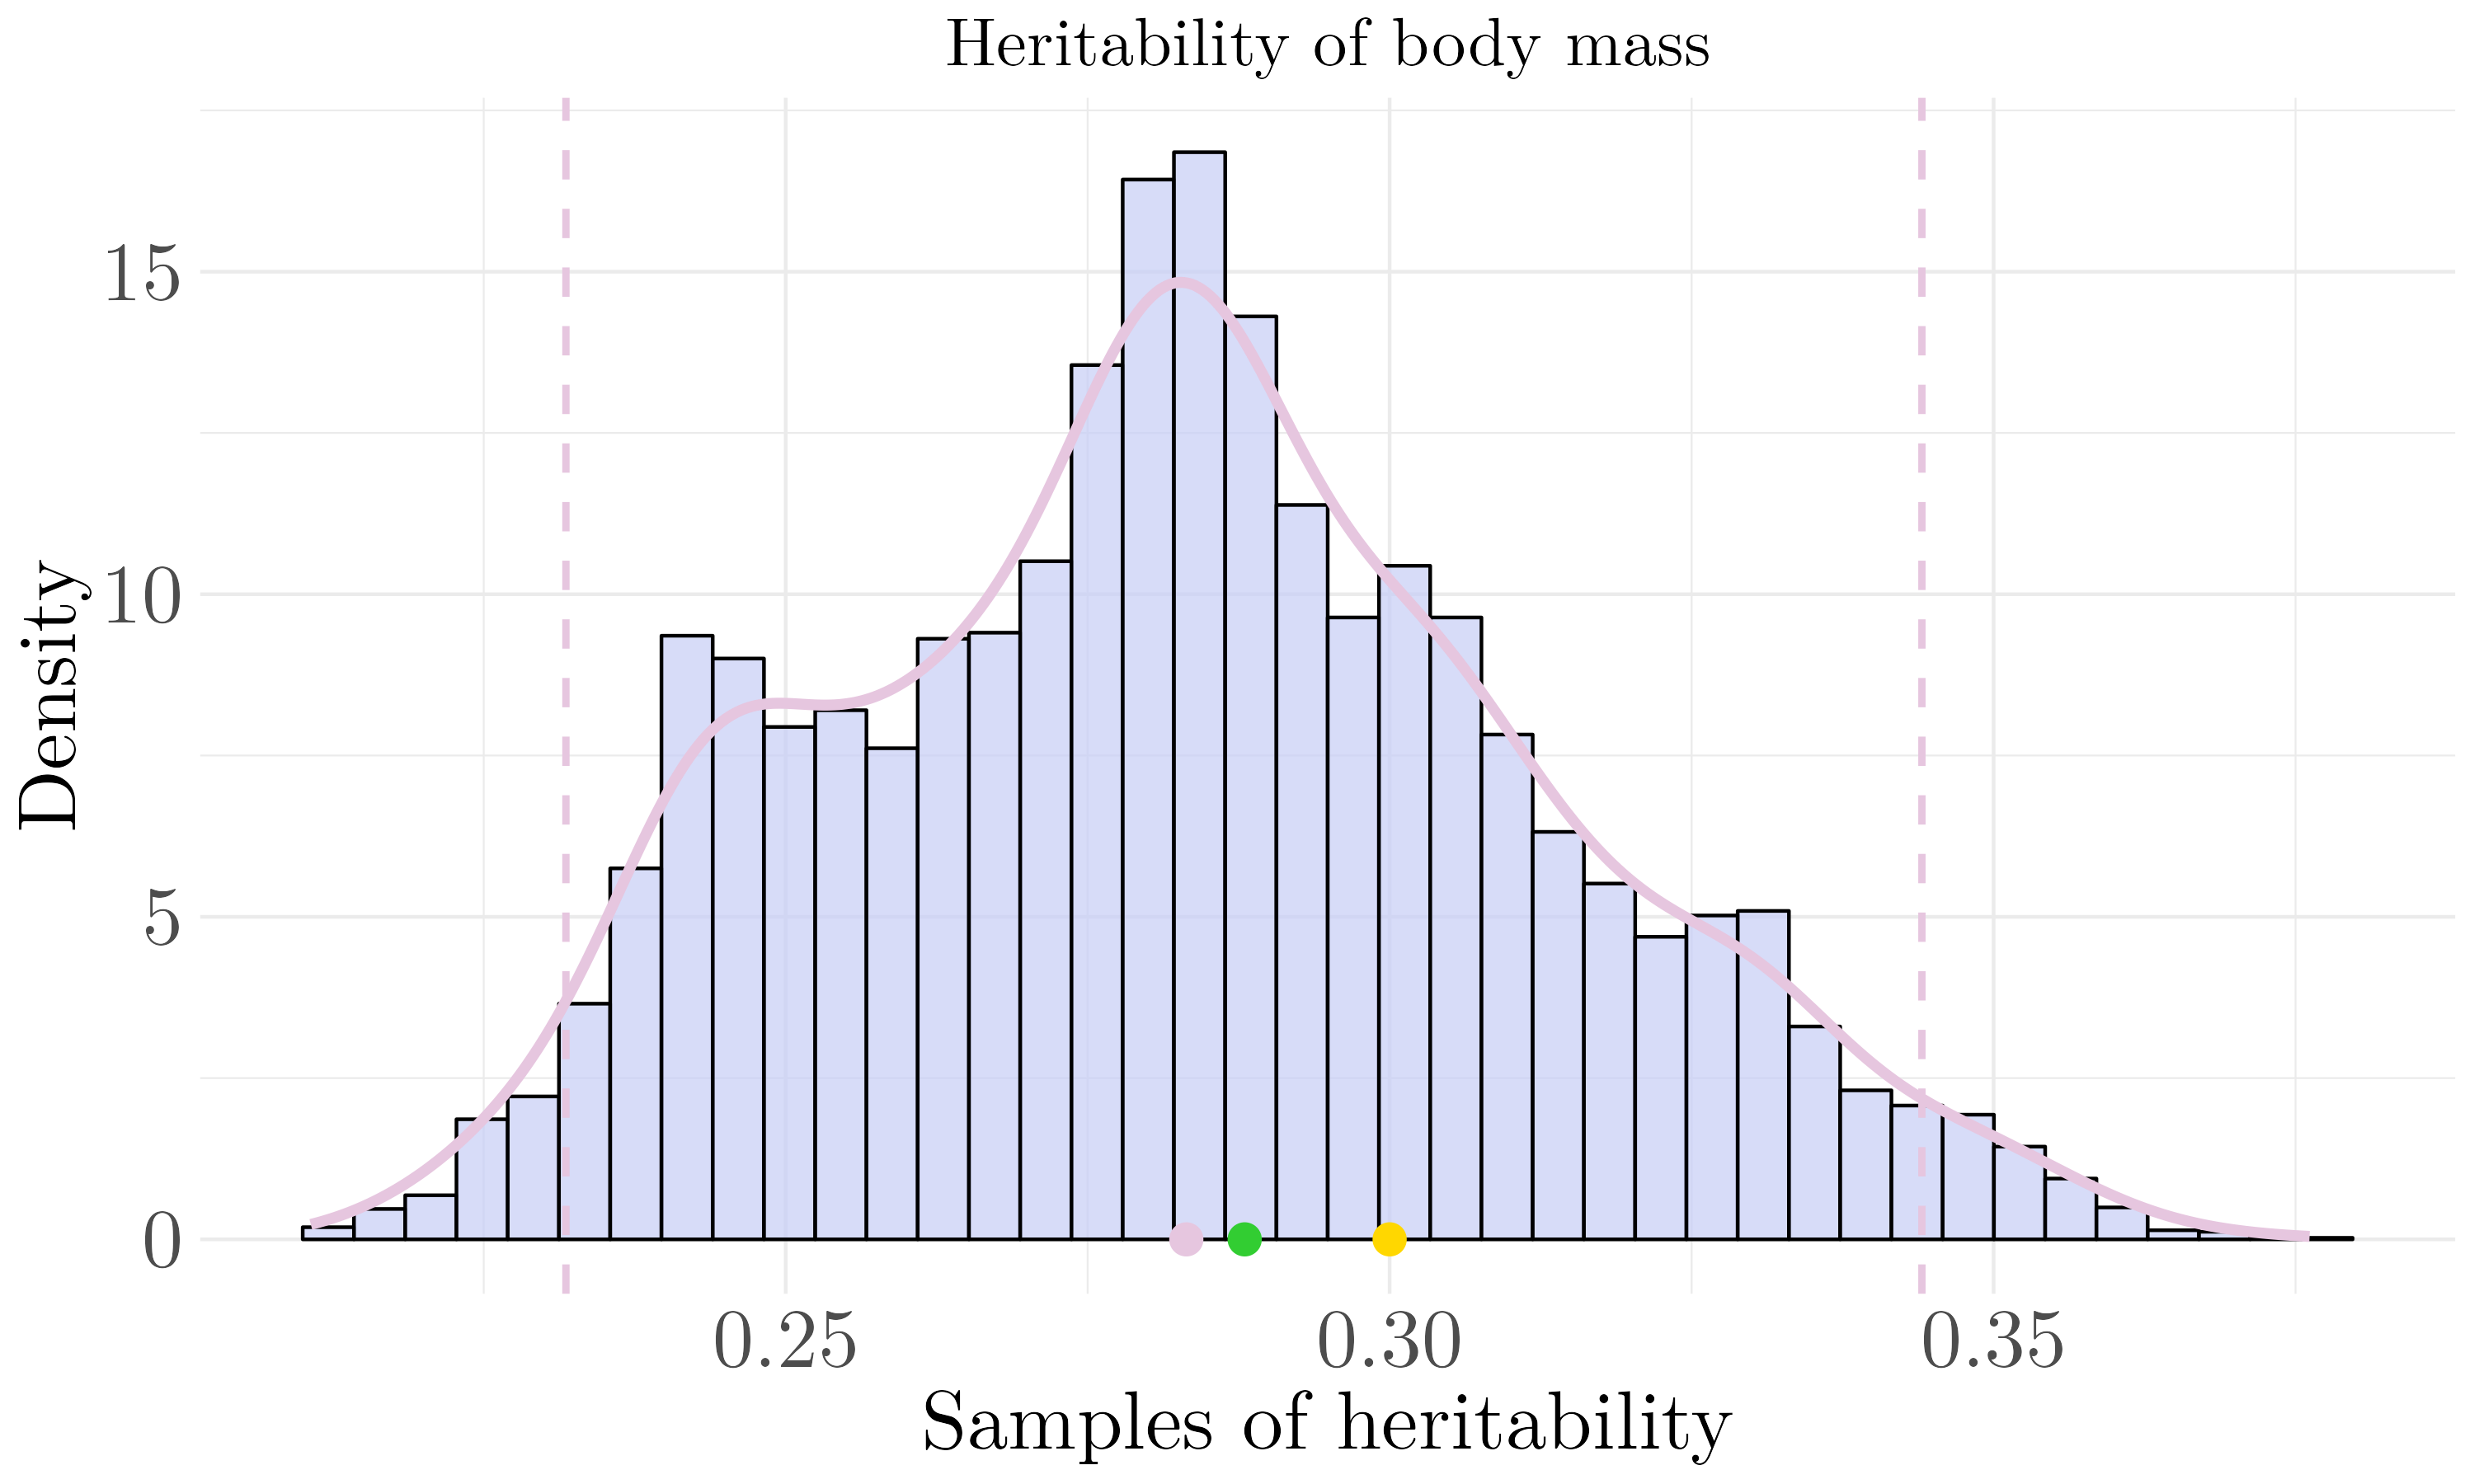
\includegraphics[width=1\linewidth]{Figures/House sparrow study/Heritability_mass.png}
    \caption{Histogram depicting the estimated heritability values of body mass by the BVI method for the house sparrow dataset. The mean of the samples is marked as a circle at the bottom of the histogram, with the lower and upper value for the $95\%$ percentile marked as dashed lines. The heritability estimate from \citet{Silva2017} and \citet{Muff2019Genetic} are marked as gold and green dots respectively at the bottom of the histogram.}
    \label{fig:heritability_mass}
\end{figure}
\noindent The samples of wing length heritability form a more symmetric curve, centered around a mean of $0.3560$ (\Cref{fig:heritability_wing} and \Cref{table:summary_heritability}). There are fewer signs of another mode for these samples, but one could argue that the right tail is a bit longer also for the heritability of wing length. The $95$th percentile is approximated by the interval $[0.3224, 0.3930]$, which is smaller than the same percentile for the body mass by a factor of $0.63$. The samples of heritability for wing length therefore exhibits less dispersion than those for heritability of body mass. In this case, the model fit and sampling procedure took $76$ seconds.
\begin{figure}[H]%\ContinuedFloat
  \centering
  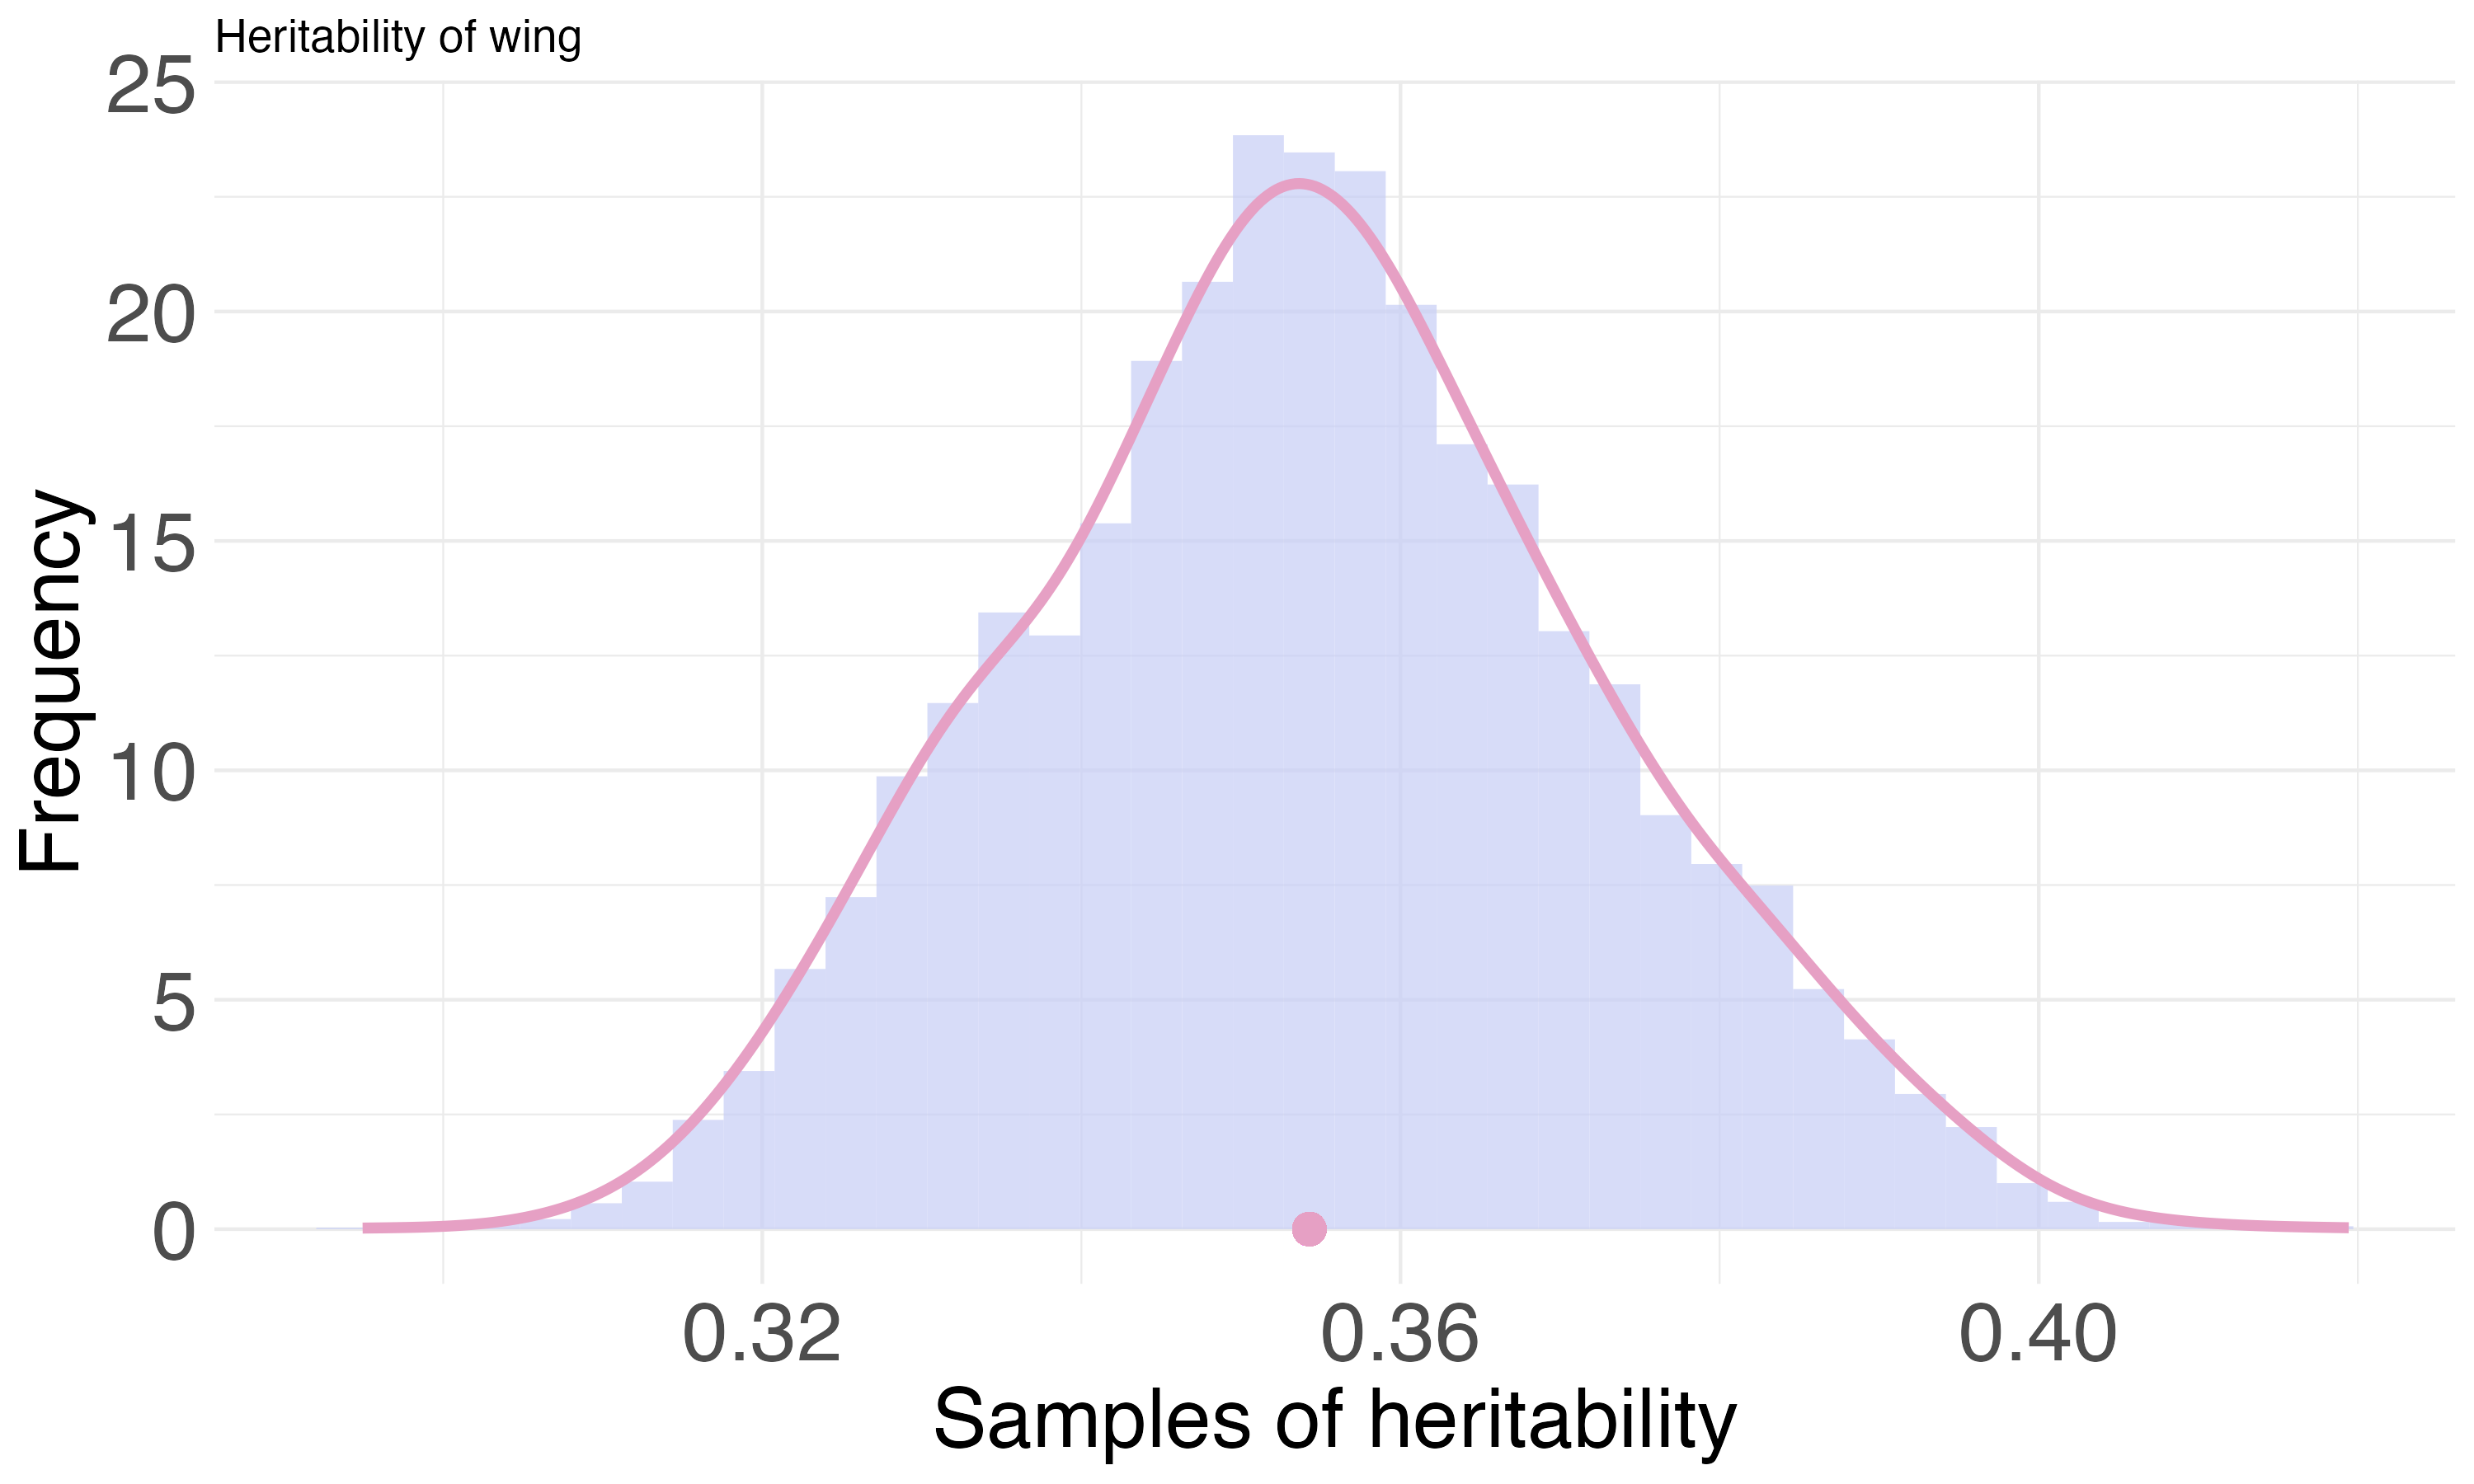
\includegraphics[width=1\linewidth]{Figures/House sparrow study/Heritability_wing.png}
  \caption{Histogram of heritability values for wing length of the house sparrows estimated by the BVI method. The mean of the samples is marked as a circle at the bottom of the histogram, and the lower and upper value for the $95\%$ percentile are featured as dashed lines. The heritability estimate from \citet{Silva2017} and \citet{Muff2019Genetic} are marked as gold and green dots respectively at the bottom of the histogram.}
  \label{fig:heritability_wing}
\end{figure}
\noindent The heritability samples of tarsus length (\Cref{fig:heritability_tarsus}) has a mean of $0.4015$ (\Cref{table:summary_heritability}) and the distribution is centered around this value. An obvious observation here is that the samples form a trimodal distribution, with three very distinct peaks. The center peak is the highest and centered around the mean and the right and left peak seem to be of equal height and symmetric about the center peak. A possible explanation for this pattern is that for this trait, the grid used for numerical integration might not be fine enough, forcing the sampling to occur most frequently at the three modal values. The $95$th percentile is captured by the interval $[0.3316, 0.4669]$ and the time spent to fit the model and draw the samples was reported to be $74$ seconds.  
\begin{figure}[H]%\ContinuedFloat
  \centering
  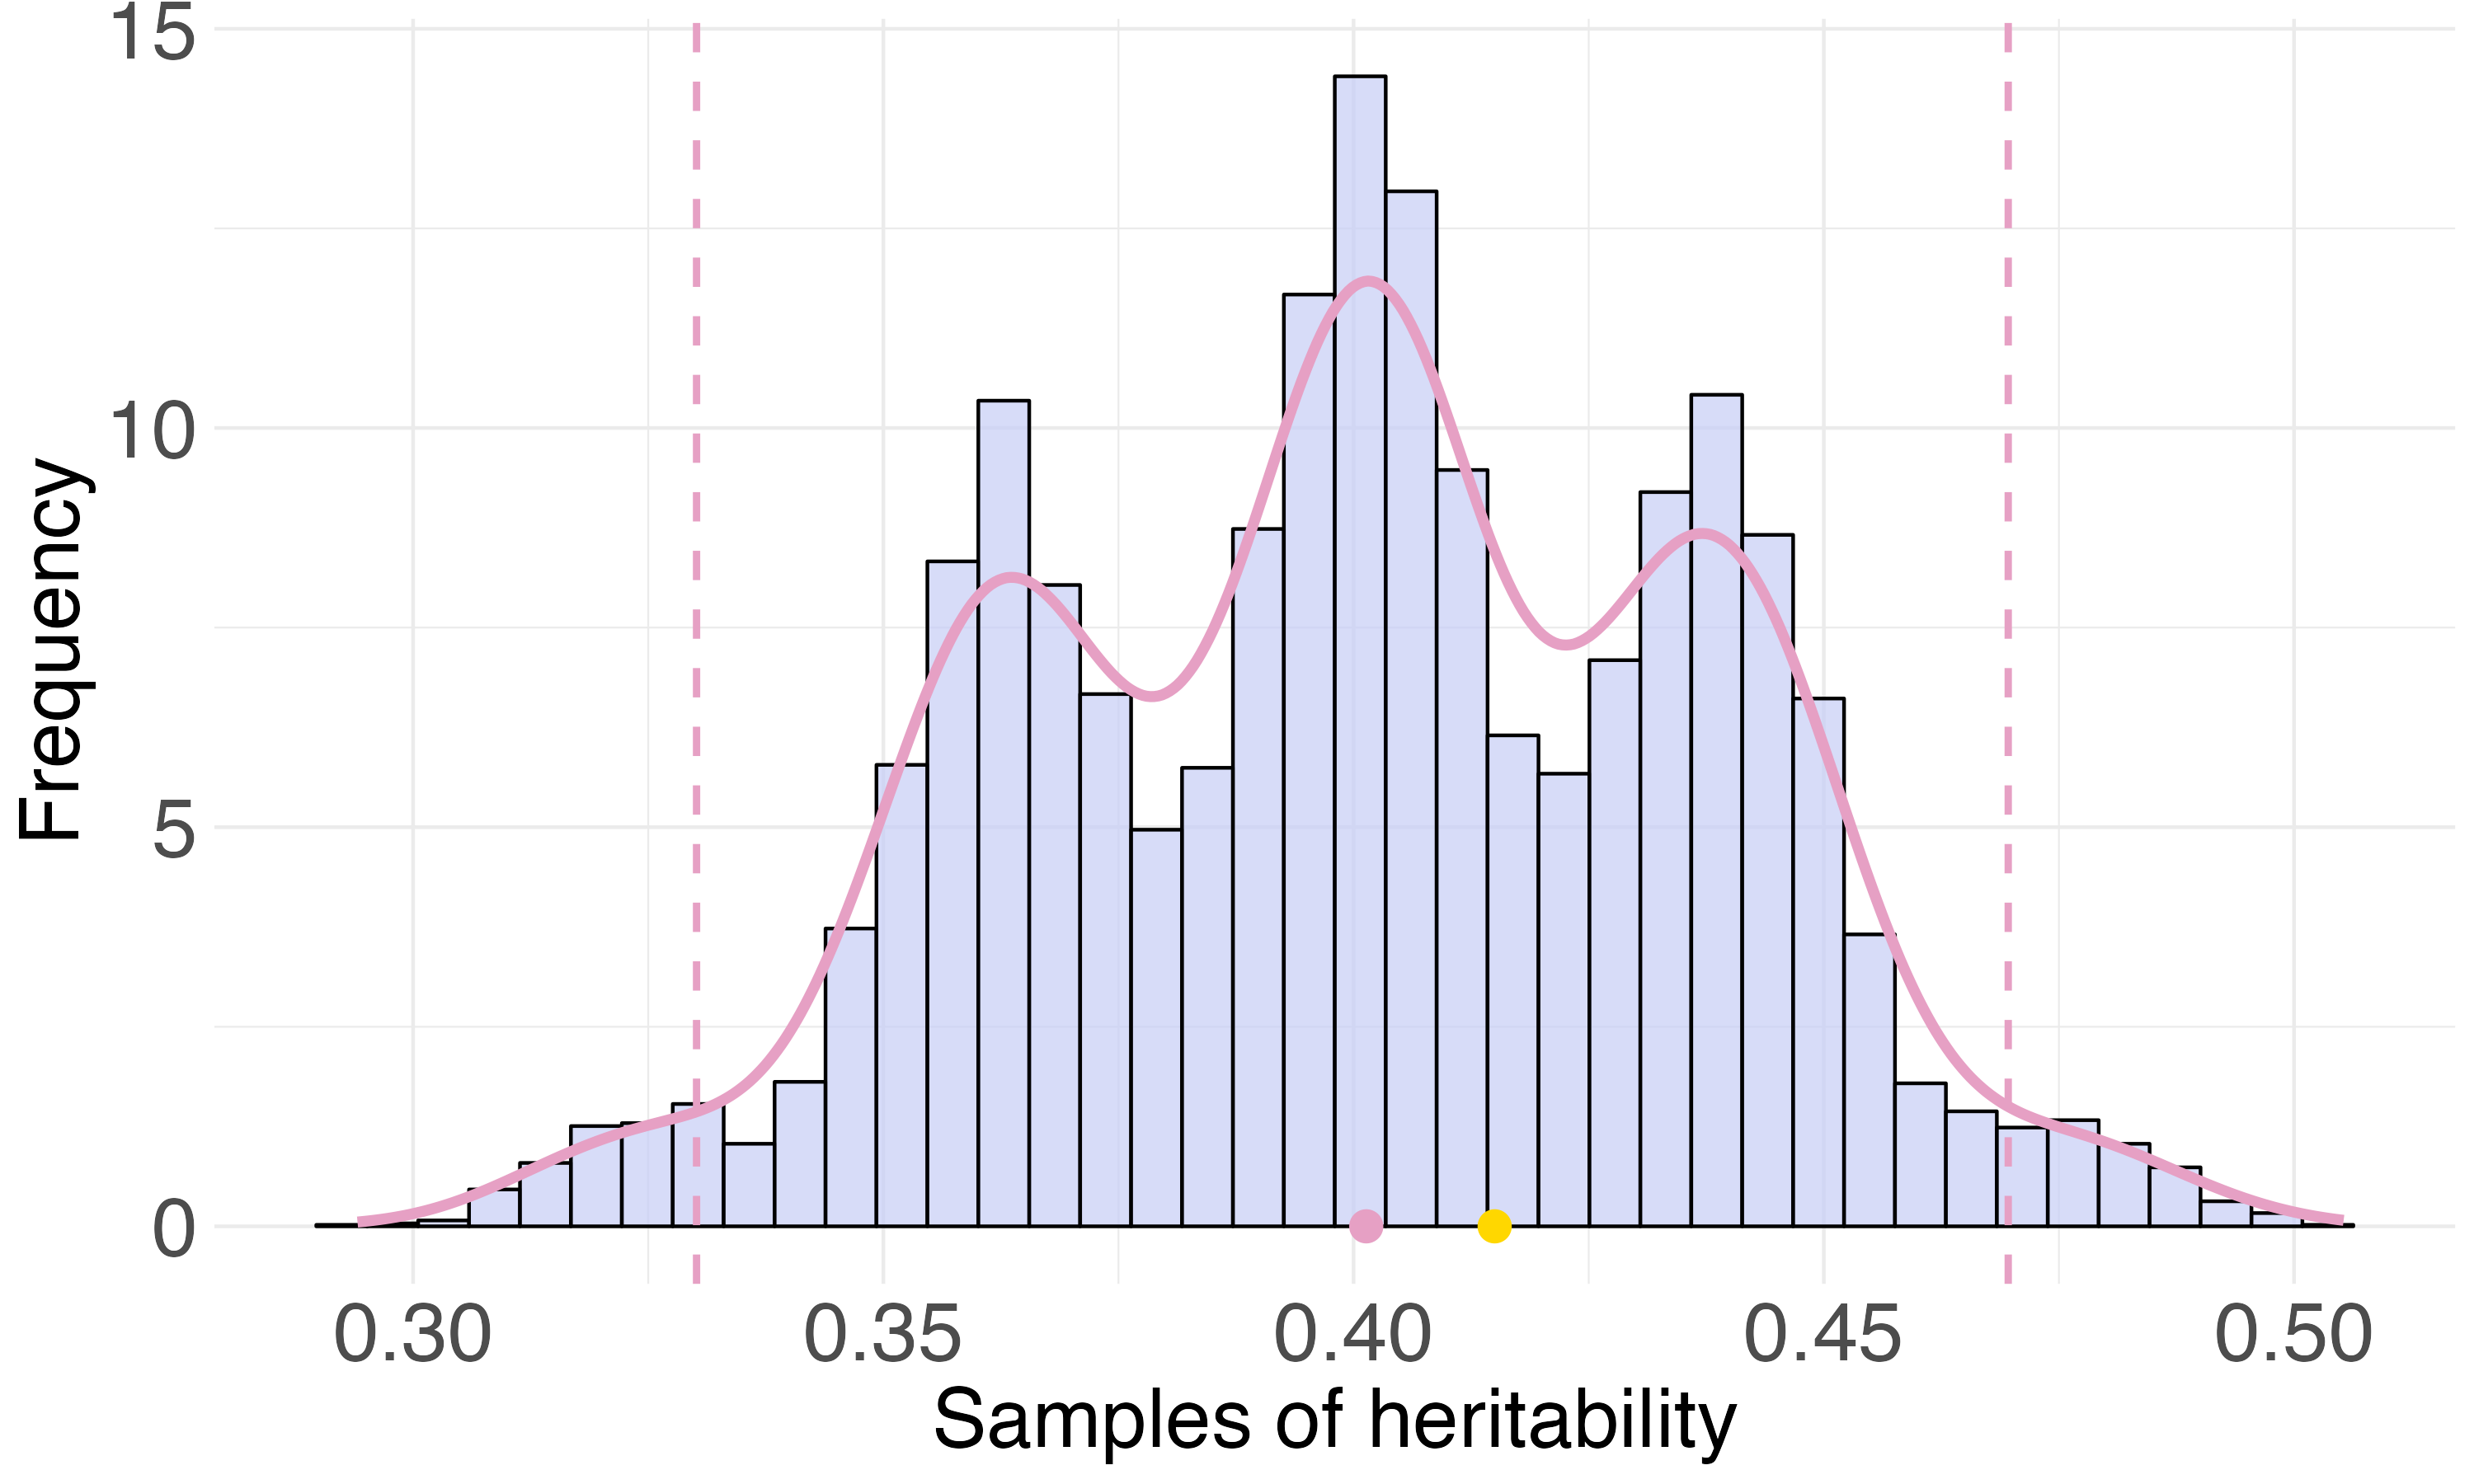
\includegraphics[width=1\linewidth]{Figures/House sparrow study/Heritability_tarsus.png}
  \caption{Histogram showing estimated heritability values for tarsus length of the house sparrows from the BVI method. The two dots at the bottom represent the mean of the samples (pink) and the estimate from \citep{Silva2017} (gold). The dashed lines represent the lower and upper value for the $95\%$ percentile.}
  \label{fig:heritability_tarsus}
\end{figure}
\noindent We see it as natural that we see different patterns that are hard to fully interpret, as the dataset is from real life and relatively small. Further, the measurements are taken on birds that are quite small, so one should expect measurement error to some degree.
  



